%%%%%%%%%%%%%%%%%%%%%%%%%%%%%%%%%%%%%%%%%
% The Legrand Orange Book
% LaTeX Template
% Version 2.1.1 (14/2/16)
%
% This template has been downloaded from:
% http://www.LaTeXTemplates.com
%
% Original author:
% Mathias Legrand (legrand.mathias@gmail.com) with modifications by:
% Vel (vel@latextemplates.com)
%
% License:
% CC BY-NC-SA 3.0 (http://creativecommons.org/licenses/by-nc-sa/3.0/)
%
% Compiling this template:
% This template uses biber for its bibliography and makeindex for its index.
% When you first open the template, compile it from the command line with the 
% commands below to make sure your LaTeX distribution is configured correctly:
%
% 1) pdflatex main
% 2) makeindex main.idx -s StyleInd.ist
% 3) biber main
% 4) pdflatex main x 2
%
% After this, when you wish to update the bibliography/index use the appropriate
% command above and make sure to compile with pdflatex several times 
% afterwards to propagate your changes to the document.
%
% This template also uses a number of packages which may need to be
% updated to the newest versions for the template to compile. It is strongly
% recommended you update your LaTeX distribution if you have any
% compilation errors.
%
% Important note:
% Chapter heading images should have a 2:1 width:height ratio,
% e.g. 920px width and 460px height.
%
%%%%%%%%%%%%%%%%%%%%%%%%%%%%%%%%%%%%%%%%%

%----------------------------------------------------------------------------------------
%	PACKAGES AND OTHER DOCUMENT CONFIGURATIONS
%----------------------------------------------------------------------------------------

\documentclass[11pt,fleqn]{book} % Default font size and left-justified equations

%----------------------------------------------------------------------------------------

\input{structure} % Insert the commands.tex file which contains the majority of the structure behind the template
\usepackage{book_sdc}


\begin{document}

%----------------------------------------------------------------------------------------
%	TITLE PAGE
%----------------------------------------------------------------------------------------

\begingroup
\thispagestyle{empty}
\begin{tikzpicture}[remember picture,overlay]
\coordinate [below=12cm] (midpoint) at (current page.north);
\node at (current page.north west)
{\begin{tikzpicture}[remember picture,overlay]
\node[anchor=north west,inner sep=0pt] at (0,0) {
\includegraphics[width=\paperwidth]{background}}; % Background image
\draw[anchor=north] (midpoint) node [fill=bluSapienza!100!white,fill opacity=1,text opacity=1,inner sep=1cm]{\color{white}\Huge\centering\bfseries\sffamily\parbox[c][][t]{\paperwidth}{\centering Continuum Mechanics\\[15pt] % Book title
{\Large Lecture Notes for  \\Nanotechnology Engineering}\\[20pt] % Subtitle
{\huge Prof.  Antonino Favata}}}; % Author name
\end{tikzpicture}};
\end{tikzpicture}
\vfill
\endgroup

%----------------------------------------------------------------------------------------
%	COPYRIGHT PAGE
%----------------------------------------------------------------------------------------

\newpage

%\vspace{5cm}
%

\vspace*{\fill}
	\noindent\textbf{Caveat lector}\\
	\noindent This draft should be regarded as a set of \textit{personal notes} for the course in \textit{Continuum Mechanics}, which I have been teaching at Sapienza University of Rome for students in Nanotechnology Engineering. The text is intentionally informal; typos, imprecisions, notational liberties, and occasional inconsistencies may be present throughout. Some parts might be quoted almost verbatim from references.\\[.5cm]
	\noindent Feedback is welcome at \texttt{antonino.favata@uniroma1.it}
	
	\vspace{.9cm}
	
%	\noindent\underline{\textbf{This draft cannot be shared without the author’s consent}}. \\
%	\noindent\underline{\textbf{Any misuse will be prosecuted in the appropriate judicial venues}}.
%	
	
\begin{tcolorbox}[colback=gray!10, colframe=black, boxrule=0.4pt, arc=2mm, width=\textwidth, left=5pt, right=5pt, top=5pt, bottom=5pt]
	\small
	\setstretch{1.5} % oppure un altro valore, es. 1.2, 1.3, 1.6...
	\textbf{This draft is intended for personal use only. Redistribution, reproduction, or public sharing without the explicit consent of the author is strictly prohibited.\\ 
		\underline{Any unauthorized use may result in legal action in the appropriate judicial venue}.}
\end{tcolorbox}
\vspace*{\fill}
~\vfill
\thispagestyle{empty}

\noindent Copyright \copyright\ 2026 Antonino Favata\\ % Copyright notice

%\noindent \textsc{Published by Publisher}\\ % Publisher

%\noindent \textsc{book-website.com}\\ % URL

%\noindent Queste note sono state utilizzate come \textit{appunti personali} per il  corso di \textit{Scienza delle Costruzioni} che  tengo presso Sapienza Università di Roma  dal  2024, per il corso di laurea triennale in Ingegneria Clinica.
%Il testo è piuttosto informale, errori di battitura, imprecisioni e abusi di notazione potrebbero essere ovunque.\\ % License information

\noindent \textit{Rome, \today} % Printing/edition date
%
%
\newpage\thispagestyle{empty}

\vspace*{\fill}
\begin{flushright}
	\raggedleft
	O voi ch'avete li 'ntelletti sani,\\
	mirate la dottrina che s'asconde\\
	sotto 'l velame de li versi strani.\footnote{O ye who have undistempered intellects,\\
		Observe the doctrine that conceals itself\\
		Beneath the veil of the mysterious verses.}\\[.4cm]
	\textsc{Dante}, \textit{Inferno} \textsc{ix}, 61-63\\[1.5cm]
	Surge ai mortali per diverse foci\\
	la lucerna del mondo [\ldots] \\
	Le cose tutte quante\\
	hanno ordine tra loro [\ldots]\footnote{To mortal men by passages diverse\\
		Uprises the world's lamp[\ldots]\\
		All things whate'er they be\\
		Have order among themselves [\ldots]}\\[.4cm]
	\textsc{Dante}, \textit{Paradiso} \textsc{i}, 37-38, 103-104\\[1.5cm]
%	Mechanicam vero duplicem Veteres constituerunt: \\ \emph{rationalem} qu\ae{} per demonstrationes accurat\ae{} procedit, \\et \emph{praticam}.\footnote{The Ancients established mechanics to be of two kinds:\ \emph{rational}, which proceeds through rigorous demonstrations, and \emph{practical}.}\\[.4cm]
	%	\textsc{Isaac Newton}
\end{flushright}
	
	\vspace{.7cm}
	
%	\begin{minipage}[t]{0.5\textwidth}
%		\raggedleft
%		\begin{tabular}{l}
%			Surge ai mortali per diverse foci\\
%			la lucerna del mondo [\ldots] \\
%			Le cose tutte quante\\
%			hanno ordine tra loro [\ldots]\\[.5cm]
%			\textsc{Dante}, \textit{Paradiso} \textsc{ixi}, 37-38, 103-104
%		\end{tabular}
%	\end{minipage}
%\end{flushright}


%\vspace{.7cm}
%
%\begin{flushright}
%	\begin{tabular}{l}
%	Mechanicam vero duplicem Veteres constituerunt: \\
%	rationalem, quae per demonstrationes accuratae procedit, \\
%	et praticam. \\[.5cm]
%		\textsc{Isaac Newton}, Philosophiae Naturalis Principia Mathematica
%	\end{tabular}
%\end{flushright}

\vspace*{\fill}

%----------------------------------------------------------------------------------------
%	TABLE OF CONTENTS
%----------------------------------------------------------------------------------------

%\usechapterimagefalse % If you don't want to include a chapter image, use this to toggle images off - it can be enabled later with \usechapterimagetrue

\chapterimage{chapter_head_1.pdf} % Table of contents heading image

\pagestyle{empty} % No headers

\tableofcontents % Print the table of contents itself

\cleardoublepage % Forces the first chapter to start on an odd page so it's on the right

\pagestyle{fancy} % Print headers again

%----------------------------------------------------------------------------------------
%	PART
%----------------------------------------------------------------------------------------

\part{Kinematics}
\chapter{General Theory}

%\section{Introduction}
It is now widely accepted that many of the advances in modern continuum mechanics are largely due to the clear distinction — made, in fact, not very long ago — between the fundamental components that form its structure: \textit{kinematics}, the \textit{balance} laws, and the \textit{constitutive} characterization of material response. These pertain to three foundational substructures upon which mechanics is built: the definition of the \textit{bodies} under investigation,\footnote{Answering questions such as what a body is in continuum physics, how one may define a part of it, or what structure the points composing the body possess — however seemingly trivial — actually requires a careful investigation of both mathematical and epistemological nature.} a geometry along with its associated \textit{kinematics}, and a theory of \textit{forces}.

The relationships among the placements of bodies, their shape, forces, and time can be of different kinds: general, such as those governing \textit{statics} — which examines putative equilibria — and \textit{dynamics} — which describes motion; or particular, namely the \textit{constitutive} relations, which define a material.

This chapter is devoted to the study of kinematics, the first pillar of the theory. We shall introduce the basic geometric notions necessary to describe bodies, their configurations in space, and their admissible motions. Emphasis will be placed on the abstract structure underlying these concepts, with the aim of providing a clear and general framework that can accommodate both classical and more advanced formulations of continuum mechanics.


\section{Deformation}
We   identify a \textit{body} $\Bc$ as a manifold of \textit{material points}, denoted by $X$. We assume that these points are primitive elements of Mechanics, in the same way that numbers are in Analysis.

We assume that a body can occupy various regions of ambient space,\footnote{Quoting Clifford Truesdell: ``Bodies are available to us only in their configurations, the regions they happen
	to occupy in Euclidean space at some time''.} which we  identify with the three-dimensional Euclidean space $\Ec$. We denote by $\Vc$ the associated vector space of translations.


We observe bodies against the framework of this spatial structure, a background that plays the role of the wall observed by the prisoners in Plato's cave. Unlike those prisoners, we are not interested in breaking our chains and running out to experience the ``real'' world, only to return to the cave and compare the shadows on the wall with their ``true'' counterparts. We simply do not consider ourselves prisoners and are instead concerned with providing a mathematical model of our only given experience, those shadows.

\begin{figure}[h!]
	\centering
	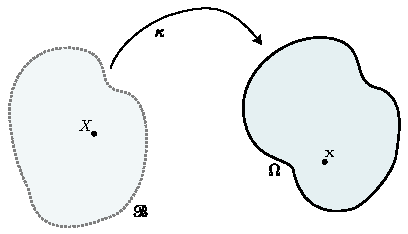
\includegraphics[scale=1.2]{figure/cinematica/piazzamento3d}
	\caption{Placement $\kappa$.}
	\label{fig:piazzamento3d}
\end{figure}
The manifold $\Bc$ is generally assumed to be regular, that is, a diffeomorphism of a domain in Euclidean space. Specifically, we state that an open set $\Omega$ in $\Ec$ is occupied by the body $\Bc$ if there exists an \textit{injective} function, called a \textit{placement} or \textit{configuration}, that maps $\Bc$ into $\Omega$:
\begin{equation}
	\kappa\,:\,\Bc\to \Omega\in \Ec.
\end{equation}
The placement $\kappa$ thus maps the material points $X$ into elements $\xb$ of the three-dimensional vector space $\Vc$; $\xb$ is therefore the position occupied by the point $X$ in the placement $\kappa$. Somewhat imprecisely, we will call $\xb$ a ``point'', meaning the position occupied by $\kappa(X)$. Similarly, we will write $\xb\in \Omega$, imagining identifying $\Omega=\fb(\Bc)$ with the set of positions of its points.

The injectivity of placements ensures that each point in Euclidean space corresponds to at most one material point. This assumption prevents the so-called ``interpenetration of matter.'' Moreover, we shall assume that placements are \textit{surjective}, meaning that for every point $\Bc$ in the set $\Omega$, there exists at least one point $\kappa(\Bc)$; in other words, the placement does not generate new points.

It follows that the placement $\kappa$ is a \textit{bijective} map and therefore admits an inverse
\begin{equation}
	\kappa^{-1}\,:\,\kappa(\Bc)=\Omega\mapsto\Bc.
\end{equation}



If $\chi$ is another placement, we can define the function
\begin{equation}
	\fb\,:\, \kappa(\Bc)\mapsto\chi(\Bc)
\end{equation}
as $\fb\coloneqq\chi\circ \kappa^{-1}$. This function is the \textit{deformation} from configuration $\kappa$ to configuration $\chi$. We observe that  $\fb$ is a vector field. Thus, if $\xb=\kappa(X)$, we say that $\xb$ and $\fb(\xb)$ are the positions occupied by the material point $X$ before and after the deformation $\fb$, respectively.

We can choose once and for all a configuration, called \textit{reference} configuration, and distinguish a second one as \textit{current}. 	When necessary, we will also distinguish $\Ecu$, $\Er$, and  $\Vcu$ $\Vr$ for the current and referential copies of $\Ec$ and $\Vc$.

\begin{figure}[h]
	\centering
	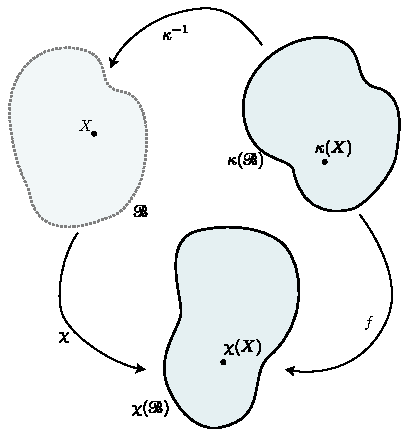
\includegraphics[scale=1.2]{figure/cinematica/def3d}
	\caption{Deformation $f$.}
	\label{fig:def3d}
\end{figure}



\subsection{Deformation Gradient}  
We assume that $\fb$ and $\fb^{-1}$ are continuous and differentiable. This circumstance avoids some pathological situations, that may occur in fracture mechanics, thal we will not consider. To infer the local effect of the deformation, we need to explore a neighborhood in a certain direction $\hb\in \Vc$, whose length $|\hb|$ will be made to tend to zero. This operation defines the directional derivative of $\fb$, which can be expressed in terms of the \textit{deformation gradient} $\partial_\xb \fb=\nabla\fb\equiv\Fb$ according to the following definition; let $\hb =\varepsilon \eb$, where $\eb$ is a unit vector and $\varepsilon=|\hb|$, we have

\begin{definition}  
	\begin{equation}  
		\lim_{\varepsilon\to0}\frac{\fb(\xb+\varepsilon \eb)-\fb(\xb)}{\varepsilon}=:\Fb(\xb)\eb.  
	\end{equation}  
\end{definition}  

This relation can be easily rewritten as  
\begin{equation}  
	\fb(\xb+\hb)-\fb(\xb)=\Fb(\xb)\hb+o(|\hb|).  
\end{equation}  
Thus, up to higher-order infinitesimals compared to $|\hb|$, the vector $\xb+\hb-\xb=\hb$ is mapped to $\Fb(\xb)\hb$.  

If $\{\eb_i\}$ is a Cartesian basis, then the deformation gradient can be written as  
\begin{equation}  
	\Fb=\fb,_{i}\otimes\eb_i.  
\end{equation}  

We require  that  
\begin{equation}\label{detpos}  
	\det \Fb(\xb)>0 \qquad\forall \xb\in\Omega.  
\end{equation}  

The physical interpretation of \eqref{detpos} is easily understood by recalling the definition of the determinant of a second-order tensor $\Ab\in\Lin$: given three non-collinear vectors $\ub, \vb,\wb\in \Vc$, the determinant of $\Ab$ is the number  
\begin{equation}\label{det}  
	\det \Ab\coloneqq \frac{\Ab\ub\times\Ab\vb\cdot\Ab\wb}{\ub\times\vb\cdot\wb}.  
\end{equation}  
The denominator on the right-hand side of \eqref{det} is the signed volume (positive if the triplet $\ub, \vb,\wb$ is positively oriented) of the parallelepiped spanned by $\ub, \vb,\wb$, while the numerator represents the signed volume of the parallelepiped spanned by $\Ab\ub, \Ab\vb,\Ab\wb$, that is, the images of the original vectors under the mapping $\Ab$. In particular, if $\Ab=\Fb$, the numerator represents the volume of the deformed parallelepiped under $\fb$. Thus, if $\det \Fb(\xb)$ were zero, it would mean that the original parallelepiped has collapsed into a point, which we want to avoid; furthermore, if it were negative, it would mean that the orientation of the original triplet has changed, which we also wish to prevent.  

Let us now explicitly write the components of the deformation gradient. By definition, we have:  
\begin{equation}  
	\begin{aligned}  
		F_{ij}=(\Fb\eb_j)\cdot \eb_i=\fb_{,j}\cdot \eb_i=f_{i,j}.  
	\end{aligned}  
\end{equation}  
The matrix representing $\Fb$ in the basis $\{\eb_i\}$ is then  
\begin{equation}  
	[\Fb]=  
	\begin{bmatrix}  
		f_{1,1}&f_{1,2}&f_{1,3}\\f_{2,1}&f_{2,2}&f_{2,3}\\f_{3,1}&f_{3,2}&f_{3,3}  
	\end{bmatrix}.  
\end{equation}  


\begin{remark}
	In order to study the deformation of $\Bc$, we can introduce two copies of the pair $(\Ec,\Vc)$, the referential pair $(\Er, \Vr)$ and the current pair $(\Ecu, \Vcu)$.
	A deformation is a map $\fb:\xb\mapsto \yb=\fb(\xb)$ from $\Er$ to $\Ecu$.  The deformation gradient $\Fb$ maps vector of $\Vr$ into $\Vcu$. Then $\Fb$ is not properly a second order tensor, since it is not a map of a space into itself; for this reason it is sometimes called \textit{double vector} or \textit{two-point tensor}.
\end{remark}

\begin{exercise}  
	Given the deformation $\fb(\xb)=\xb+\alpha x_2\eb_2+\beta x_2x_3\eb_3$, with $\xb=x_1\eb_1+x_2\eb_2+x_3\eb_3$. Determine the deformation gradient.  
	\begin{svolgimento}  
		The components of the deformation are:  
		\begin{equation}  
			\begin{aligned}  
				&f_{1}=\fb\cdot \eb_{1}=x_{1},\\  
				&f_{2}=\fb\cdot \eb_{2}=x_{2}+\alpha x_{2},\\  
				&f_{3}=\fb\cdot \eb_{3}=x_{3}+\beta x_{2}x_{3},  
			\end{aligned}  
		\end{equation}  
		from which we immediately obtain  
		\begin{equation}  
			[\Fb]=  
			\begin{bmatrix}  
				f_{1,1}&f_{1,2}&f_{1,3}\\f_{2,1}&f_{2,2}&f_{2,3}\\f_{3,1}&f_{3,2}&f_{3,3}  
			\end{bmatrix}=  
			\begin{bmatrix}  
				1&0&0\\0&1+\alpha&0\\0&\beta x_3&1+\beta x_2  
			\end{bmatrix}.  
		\end{equation}  
		Without resorting to the matrix representation, we can immediately write:  
		\begin{equation}  
			\Fb=\fb_{,i}\otimes\eb_i=\eb_1\otimes\eb_1+(1+\alpha)\eb_2\otimes\eb_2+\beta x_3\eb_3\otimes\eb_2+(1+\beta x_2)\eb_3\otimes\eb_3.  
		\end{equation}  
	\end{svolgimento}  
\end{exercise}  


\subsection{Displacement}  
If $\xb$ and $\fb(\xb)$ are, respectively, the positions occupied by a material point in two placements, their difference defines the displacement vector:  
\begin{definition}  
	\begin{equation}  
		\ub(\xb)\coloneqq\fb(\xb)-\xb.  
	\end{equation}  
\end{definition}  

\begin{figure}  
	\centering  
	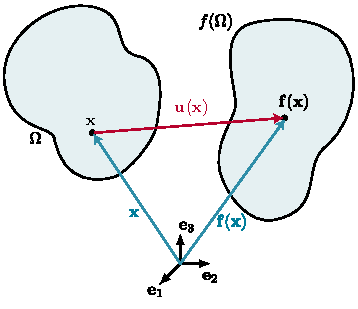
\includegraphics[scale=1.2]{figure/cinematica/displ}  
	\caption{Displacement vector.}  
	\label{fig:displ}  
\end{figure}  

Its gradient, which we denote by $\Hb\coloneqq\nabla\ub$, is given by  

\begin{definition}  
	\begin{equation}\label{HFI}  
		\Hb(\xb)=\Fb(\xb)-\Ib,  
	\end{equation}  
\end{definition}  
where $\Ib$ is the identity tensor. If $\{\eb_i\}$ is a Cartesian basis, then  
\begin{equation}  
	\Hb=\ub,_i\otimes\eb_i  
\end{equation}  
and the components of $\Hb$ are immediately obtained as  
\begin{equation}  
	H_{ij}=\Hb\eb_j\cdot\eb_i=u_{i,j}.  
\end{equation}  

\begin{remark}
The condition \eqref{detpos}   becomes particularly clear in a one-dimensional context. Let us therefore consider a continuum embedded in a one-dimensional Euclidean space, aligned with the direction $\eb$. A point is then given by $\xb = x\eb$, the deformation by $\fb(x) = f(x)\eb$, and the displacement by $\ub(x) = u(x)\eb = (f(x) - x)\eb$. In this elementary setting, condition \eqref{detpos}   translates into the requirement that $f'>0$, that is, the deformation must be monotonically increasing.

Let $L$ denote the length of the domain $\Omega$, whose endpoints we label as points $A$ and $B$; the assumption of monotonicity for the deformation becomes the condition
\begin{equation}
	u'(x) > -1,
\end{equation}
which, when integrated over $\Omega$, yields the inequality
\begin{equation}
	u(L) > u(0) - L.
\end{equation}
If this inequality were not satisfied, then after the deformation point $B$ could end up to the left of point $A$. In other words, the oriented segment $\big( x(B)-x(A) \big)\eb$, which in the undeformed configuration pointed from $A$ to $B$ along the direction $\eb$, could be deformed into a segment oriented in the opposite direction, leading to interpenetration of matter.

\begin{center}
	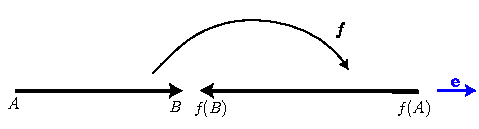
\includegraphics[scale=1.3]{figure/cinematica/orient1d}
\end{center}

We therefore say that the condition $f'(x) > 0$ ensures the preservation of spatial orientation (segments initially oriented along $\eb$ remain so) and the prevention of interpenetration of matter. Finally, observe that the inequality must be strict: if we had $u(L) - u(0) = -L$, the endpoints of the segment would collapse into a single point—an outcome we seek to avoid.
\end{remark}

\section{Change in Length}  
Let us consider, in a reference configuration, two 'nearby' points $\xb$ and $\xb_0$. The infinitesimal segment they define has a length  
\begin{equation}  
	d\ell_0=|\xb-\xb_0|.  
\end{equation}  
Denoting by $\tb$ the unit vector that defines the direction,  
\begin{equation}  
	\tb\coloneqq\frac{\xb-\xb_0}{|\xb-\xb_0|},  
\end{equation}  
we can write  
\begin{equation}  
	\xb-\xb_0=d\ell_0 \tb.  
\end{equation}  
The images of $\xb$ and $\xb_0$ under the deformation are $\fb(\xb)$ and $\fb(\xb_0)$, which define a segment of length  
\begin{equation}  
	d\ell:=|\mathbf{f}(\mathbf{x})-\mathbf{f}(\mathbf{x}_0)|.  
\end{equation}  

\begin{center}  
	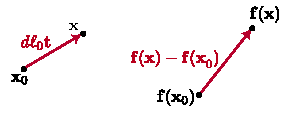
\includegraphics[scale=1.2]{figure/cinematica/dl}  
\end{center}  

Expanding the deformation in a Taylor series around $\xb_0$, we have  
\begin{equation}  
	\mathbf{f}(\mathbf{x})=\mathbf{f}(\mathbf{x}_{0})+\mathbf{F}(\mathbf{x}_{0})[\mathbf{x-x}_{0}]+o(|\mathbf{x-x}_{0}|),  
\end{equation}  
or equivalently,  
\begin{equation}  
	\mathbf{f}(\mathbf{x})-\mathbf{f}(\mathbf{x}_0)=d\ell_0\mathbf{F}\mathbf{t}+o(d\ell_0),  
\end{equation}  
from which it follows that  
\begin{equation}  
	d\ell=|\mathbf{f}(\mathbf{x})-\mathbf{f}(\mathbf{x}_0)|=d\ell_0|\mathbf{F}\mathbf{t}|+o(d\ell_0).  
\end{equation}  
Thus, up to higher-order infinitesimals of order $o(d\ell_0)$, the ratio between the two lengths is given by  
\begin{definition}  
	\begin{equation}\label{dl}  
		\frac{d\ell}{d\ell_0}=|\mathbf{Ft}|.  
	\end{equation}  
\end{definition}  

We have therefore concluded that, given an infinitesimal segment in the direction $\tb$ in the reference configuration, the ratio between the length of the deformed segment and the length of the undeformed segment equals the norm of the deformation gradient applied to $\tb$.  

Observe that $|\mathbf{Ft}|$ can be rewritten as  
\begin{equation}  
	|\mathbf{Ft}|=\sqrt{\Fb\tb\cdot\Fb\tb}=\sqrt{\Fb^\top\Fb\tb\cdot\tb}.  
\end{equation}  
Introducing the \textit{right Cauchy-Green tensor},  
\begin{definition}  
	\begin{equation}  
		\Cb\coloneqq\Fb^\top\Fb,  
	\end{equation}  
\end{definition}  
the ratio between the deformed and undeformed segment lengths can alternatively be written as  
\begin{equation}  
	\frac{d\ell}{d\ell_0}=\sqrt{\Cb\tb\cdot\tb}.  
\end{equation}  

\begin{remark}  
	It is interesting to note that $\Cb^\top=(\Fb^\top\Fb)^\top=\Fb^\top\Fb=\Cb$, so $\Cb$ is symmetric. This observation suggests that, to evaluate length variations, it is not necessary to know the entire deformation gradient $\Fb$, which generally has nine components. It is sufficient to know $\Cb$, which is characterized by six components. This implies that the deformation gradient $\Fb$ contains more information than $\Cb$, but this additional information is not required to describe length variations. It is not difficult to infer that the extra information concerns the rigid component of the deformation, as we will see later.  
\end{remark}  



\section{Change in Area}



Let us now consider  three non collinear points $\xb_0$, $\xb_0+\ab$, $\xb_0+\bb$ in the reference configuration, $\ab$, $\bb$ infinitesimal.
The vectors $\ab$ and $\bb$ define the oriented surface whose normal is
\begin{equation}
	\nb_{\rm ref}=\frac{\ab\times\bb}{|\ab\times\bb|};
\end{equation}
 the quantity
\begin{equation}
	da_0=|\ab\times\bb|
\end{equation}
 is a measure of the area of the oriented surface. In the deformed configuration, the area of the deformed surface is
 \begin{equation}
 da=|\Fb \ab \times \Fb \bb|
 \end{equation}
 and the deformed normal vector is 
 \begin{equation}
 \nb_{\rm cur}=\frac{\Fb \ab \times \Fb \bb}{|\Fb \ab \times \Fb \bb|}.
 \end{equation}
 We need to relate $ \nb_{\rm ref}$ and $ \nb_{\rm cur}$
 
To do this, we need some algebra. In particular, we recall that the determinant is an operator that assigns to each second order tensor $\Ab$ a scalar $\det\Ab$ defined by
\begin{equation}\label{det}
	\det\Ab=\frac{\Ab\ub\cdot(\Ab\vb\times \Ab\wb)}{\ub\cdot(\vb\times \wb)},
\end{equation}
for any basis $\{\ub,\vb,\wb\}$. It is easy to see then that $|\det\Ab|$ is the ratio of the volume of the parallelepiped defined by the vectors $\Ab\ub$, $\Ab\vb$ and $\Ab\wb$ to the volume of the parallelepiped defined by the vectors $\{\ub,\vb,\wb\}$. 

Now let $\Ab$ invertible and let define $\bar\ub=\Ab \ub$; therefore the following equality holds for all $\bar{\ub}$:
\begin{equation}
\bar{\ub} \cdot( \Ab \vb\times\Ab\wb)=(\det\Ab)\Ab^{-1} \bar{\ub}\cdot (\vb\times\wb)=(\det\Ab)\bar{\ub}\cdot\Ab^{-\top}(\vb\times\wb),
\end{equation}
 whence we deduce that
%
%
%
%Now, let
%\begin{equation}
%	\ab:=\Ab \ub\times\Ab \vb;
%\end{equation}
%since $\Ab\ub\cdot \ab=\Ab\vb\cdot\ab=0$, it follows that $\Ab^\top\ab$ is orthogonal to $\ub$ and $\vb$ and then there exist $\gamma\in\Ro$ such that
%\begin{equation}
%	\Ab^\top\ab=\gamma(\ub\times\vb) \quad \Longrightarrow \quad\Ab^\top(\Ab\ub\times\Ab\vb)=\gamma(\ub\times\vb).
%\end{equation}
%Let $\wb=\ub\times\vb$; then
%\begin{equation}
%	\gamma\wb\cdot(\ub\times\vb)=\wb\cdot\Ab^\top(\Ab\ub\times\Ab\vb)=\Ab\wb\cdot (\Ab\ub\times\Ab\vb).
%\end{equation}
%This latter relation reveals that $\gamma=\det\Ab$ and then
%\begin{equation}
%	\Ab^\top(\Ab\ub\times\Ab\vb)=\det\Ab(\ub\times\vb),
%\end{equation}
%or rather
\begin{equation}\label{cofactor}
	\Ab \vb\times \Ab \wb =\Ab^*(\vb\times\wb), \quad \Ab^*:=(\det\Ab)\Ab{^{-\top}}.
\end{equation}
The tensor $\Ab^*$ is the cofactor of $\Ab$. With \eqref{cofactor}, the current normal vector becomes
\begin{equation}
	\nb_{\rm cur}=\frac{\Fb\ab\times\Fb\ab}{|\Fb\ab\times\Fb\ab|}=\frac{\Fb^*\nb_{\rm ref}}{|\Fb^*\nb_{\rm ref}|},
\end{equation}
whence we deduce the
\begin{definition}
	 \textit{\textbf{Nanson formula}}
	\begin{equation}\label{nanson}
\frac{da}{da_0}\,\nb_{\rm cur}=\Fb^*\nb_{\rm ref},
\end{equation}
\end{definition}
and then

\begin{definition}
	\begin{equation}
	\frac{da}{da_0}=|\Fb^*\nb_{\rm ref}|.
\end{equation}
\end{definition}

\begin{exercise}
Prove that the change in area can be expressed in terms of the right Cauchy-Green tensor.
\end{exercise}

\section{Change in Volume}  
Let us now consider four points $\xb_0$, $\xb_0+\ab$, $\xb_0+\bb$, $\xb_0+\cb$ in the reference configuration, with $\ab$, $\bb$, $\cb$ infinitesimal. The vectors $\ab$, $\bb$, and $\cb$  determine a parallelepiped with volume
\begin{equation}
dv_0=|\ab \cdot \bb \times \cb|.
\end{equation} 
The volume of the deformed parallelepiped is
\begin{equation}
dv=|\Fb\ab \cdot \Fb\bb \times \Fb\cb|,
\end{equation}
whence
\begin{definition}
	\begin{equation}
\frac{dv}{dv_0}=\frac{|\Fb\ab \cdot \Fb\bb \times \Fb\cb|}{|\ab \cdot \bb \times \cb|}=\det \Fb.
\end{equation}
\end{definition}

\begin{exercise}
	Prove that the change in volume can be expressed in terms of the right Cauchy-Green tensor.
\end{exercise}

\section{Homogeneous Deformations}

A deformation is said to be \textit{homogeneous} if its gradient is constant. In particular, the following representation holds:

\begin{definition}
	\begin{equation}
		\fb(\xb)=\fb(\xb_0)+\Fb(\xb-\xb_0),
	\end{equation}
\end{definition}
with constant $\Fb$. Examples of homogeneous deformations include \textit{translations}:
\begin{equation}
	\fb(\xb)=\xb +\cb,
\end{equation}
with constant $\cb$. In this deformation, every point is translated by the vector~$\cb$.

Another relevant example is given by \textit{rotations}, that is, deformations of the form
\begin{equation}
	\fb(\xb)=\xb_0+\Rb(\xb-\xb_0),
\end{equation}
with $\Rb\in\Rot$ and $\xb_0\in\Vc$; such a deformation rotates the body around the point $\xb_0$, as specified by the orthogonal tensor $\Rb$.

\begin{exercise}
	Given a Cartesian reference frame $\{\eb_i\}$, consider the effect of a rotation about the $\eb_3$ axis through the origin on the basis vectors.
	
	\begin{svolgimento}
		This is a homogeneous deformation given by
		\begin{equation}
			\fb(\xb)=\Rb\xb,
		\end{equation}
		with gradient $\Fb=\Rb$. The matrix representation of the rotation is
		\begin{equation}\label{Rp}
			[\Rb]=\begin{bmatrix}\cos\theta&-\sin\theta&0\\\sin\theta&\cos\theta&0\\0&0&1\end{bmatrix}.
		\end{equation}
		It is then straightforward to verify the effect on the basis vectors:
		\begin{equation}
			\Fb\eb_1=\Rb\eb_1=\cos\theta\eb_1-\sin\theta\eb_2, \quad \Fb\eb_2=\Rb\eb_2=\sin\theta\eb_1+\cos\theta\eb_2,  \quad 
			\Fb\eb_3=\Rb\eb_3=\eb_3.
		\end{equation}
	\end{svolgimento}
\end{exercise}

A deformation is said to be \textit{rigid} if it preserves mutual distances between points, that is,
\begin{equation}\label{fxfz}
	|\mathbf{f}(\mathbf{x})-\mathbf{f}(\mathbf{z})|=|\mathbf{x}-\mathbf{z}|\quad\forall\mathbf{x},\mathbf{z}\in\Omega.
\end{equation}
Let us examine the consequences of this condition.

Before doing so, we derive a useful result in the following exercise.

\begin{exercise}\label{gradab}
	Let $\ab(\xb)$ and $\bb(\xb)$ be two vector fields. Determine the gradient of $\ab(\xb)\cdot\bb(\xb)$.
	
	\begin{svolgimento}
		The gradient we seek is
		\begin{equation}
			\nabla\big( \ab(\xb)\cdot\bb(\xb) \big)=\partial_\xb\big( \ab(\xb)\cdot\bb(\xb) \big).
		\end{equation}
		It is convenient to work in components. Omitting the explicit dependence of the fields on $\xb$, we get
		\begin{equation}
			\begin{aligned}
				\nabla\big( \ab\cdot\bb\big)=\partial_\xb\big( \ab\cdot\bb \big)&=(a_i b_i),_{j}=a_{i,j}b_i+a_ib_{i,j}=(a_{j,i})^\top b_i+(b_{j,i})^\top a_i\\
				&=(\nabla\ab)^\top\bb+(\nabla \bb)^\top\ab.
			\end{aligned}
		\end{equation}
	\end{svolgimento}
	
\end{exercise}

Equation~\eqref{fxfz} is equivalent to requiring
\begin{equation}
	\left(\mathbf{f}(\mathbf{x})-\mathbf{f}(\mathbf{z})\right)\cdot\left(\mathbf{f}(\mathbf{x})-\mathbf{f}(\mathbf{z})\right)=(\mathbf{x}-\mathbf{z})\cdot(\mathbf{x}-\mathbf{z})\quad\forall\mathbf{x},\mathbf{z}\in\Omega.
\end{equation}
Differentiating with respect to $\xb$, and using the result from Exercise~\ref{gradab}, we find
\begin{equation}
	2	\Fb^\top(\xb)\fb(\xb)-2\Fb^\top(\xb)\fb(\zb)=2\xb-2\zb  \quad\forall\mathbf{x},\mathbf{z}\in\Omega;
\end{equation}
differentiating now with respect to $\zb$, we obtain
\begin{equation}
	\Fb^\top(\xb)\Fb(\zb)=\Ib.
\end{equation}
This implies that $\Fb$ does not depend on the point and is an orthogonal tensor. Since $\det\Fb>0$, it follows that it is a rotation.

We then conclude that rigid deformations have the following general representation:

\begin{definition}
	\begin{equation}
		\begin{aligned}
			\mathbf{f}(\mathbf{x}) &= \mathbf{f}(\mathbf{x}_0)-\mathbf{x}_0 &&\text{translation of the generic point }\mathbf{x}_0, \\
			&\quad+\mathbf{x}_0+\mathbf{Q}(\mathbf{x}-\mathbf{x}_0)&&\text{rotation about the point }\mathbf{x}_0,
		\end{aligned}
	\end{equation}
\end{definition}
with $\Qb \in \Rot$.  
In other words, a rigid deformation is the composition of a translation and a rotation (i.e., a \textit{rigid-body deformation} ).





\section{Strain Measures}
We have already observed that, to measure geometric  changes, it is not necessary to know the full strain gradient $\Fb$, which generally has 9 components, but only the right Cauchy-Green tensor $\Cb$. We have also seen that $\Cb$ is symmetric and it is immediate to verify that it is also positive definite.\footnote{In fact, for any $\ab\in\Vc$
	\begin{equation}
		\Cb \ab\cdot\ab = \Fb \ab\cdot\Fb\ab = |\Fb\ab|^2 \geq 0.
	\end{equation}
	Moreover, $\Cb \ab\cdot\ab = 0$ if and only if $|\Fb \ab| = 0$, which is true if and only if $\Fb \ab = \mathbf{0}$; but $\det \Fb > 0$, so $\Fb\ab = \mathbf{0}$ if and only if $\ab = \mathbf{0}$. Therefore,
	\begin{equation}
		\Cb \ab\cdot\ab > 0 \quad \forall \ab \neq \mathbf{0}.
	\end{equation}
}
By the spectral theorem, $\Cb$ can be represented as
\begin{equation}
	\Cb = \sum_{i=1}^3 \lambda_i \cb_i \otimes \cb_i,
\end{equation}
where the eigenvalues $\lambda_i$ are positive. We can then define the tensor
\begin{definition}
	\begin{equation}
	\Ub \coloneqq \sum_{i=1}^3 \sqrt{\lambda_i} \cb_i \otimes \cb_i,
\end{equation}
\end{definition}
that is, $\Cb = \Ub \Ub = \Ub^2$. The tensor $\Ub$, called the \textit{right deformation tensor}, is obviously symmetric and positive definite, and is the sum of three extensions in three orthogonal directions. We define
\begin{equation}
	\Rb = \Fb \Ub^{-1}.
\end{equation}
The tensor $\Rb$ is clearly a rotation. In fact,
\begin{equation}
	\mathbf{R}^\top \mathbf{R} = \mathbf{U}^{-1} \mathbf{F}^\top \mathbf{F} \mathbf{U}^{-1} = \mathbf{U}^{-1} \mathbf{C} \mathbf{U}^{-1} = \mathbf{U}^{-1} \mathbf{U} \mathbf{U} \mathbf{U}^{-1} = \mathbf{I}.
\end{equation}

Thus, the following decomposition, called \textit{polar decomposition}, holds:
\begin{definition}
	\begin{equation}\label{polar}
		\Fb = \Rb \Ub.
	\end{equation}
\end{definition}
where $\Rb$ is a rotation and $\Ub$ is a pure deformation (see Fig. \ref{fig:polar}). The representation \eqref{polar} clearly shows that $\Fb$ contains a part that is a rotation, and thus not responsible for length variations.
%
\begin{figure}[h!]
	\centering
	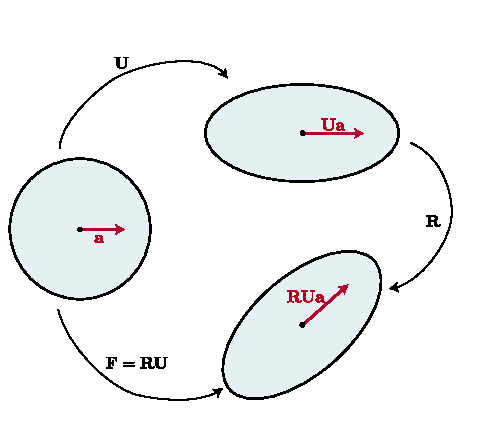
\includegraphics[scale=1.2]{figure/cinematica/polar}
	\caption{Effect of the polar decomposition. The action of $\Fb$ on the vector $\ab$ can be decomposed as the action of a pure deformation $\Ub$ followed by a rotation $\Rb$.}
	\label{fig:polar}
\end{figure}
%
In this sense, $\Fb$ \textit{is not} a good \textit{measure of strain}. The tensors $\Cb$ and $\Ub$ are instead suitable for describing the shape changes of bodies associated with metric variations. However, they do not vanish in the case of rigid deformations. In fact, if $\Fb = \Rb$, then $\Cb = \Ub = \Ib$. Since it makes sense to define the strain measure as a defect of rigidity, we introduce the \textit{Green--Saint-Venant tensor}
\begin{definition}
	\begin{equation}
		\Eb_{\rm G} \coloneqq \frac{1}{2}(\Cb - \Ib),
	\end{equation}
\end{definition}
which corresponds to a rigid deformation with the null tensor. The factor $1/2$ does not have a physical meaning, but it will be convenient later.


Analogously, we can introduce the  \textit{ left polar decomposition}
\begin{definition}
\begin{equation}
	\Fb=\Vb\Rb
\end{equation}
\end{definition}
where 
\begin{equation}
 \Vb=\sqrt{\Fb\Fb^\top}.
\end{equation}
is \textit{left stretch tensor}. The tensor
\begin{equation}
\Bb=\Vb^2= \Fb\Fb^\top
\end{equation}
is the  \textit{left Cauchy--Green} (deformation) tensor.




\section{Deformation in curvilinear coordinates}
	Let us consider a set of curvilinear coordinates $\zeta^i$ $(i=1,2,3)$ for a point $\xb\in\Vr$:
	\begin{equation}
		(\zeta^1,\zeta^2,\zeta^3)\mapsto \xb=\widehat{\xb}(\zeta^1,\zeta^2,\zeta^3), \qquad \xb\mapsto\zeta^i=\widehat{\zeta}^i (\xb)\;(i=1,2,3),
	\end{equation}
	with
	\begin{equation}
		\widehat{\xb}\big(\widehat\zeta^1(\xb),\widehat\zeta^2(\xb),\widehat\zeta^3(\xb)\big)=\xb.
	\end{equation}
	Let $\yb$ be the image of $\xb$ under the deformation $\fb$. To the point $\yb$ we associate the same set of curvilinear coordinates $\zeta^i$ $(i=1,2,3)$:
	\begin{equation}
		(\zeta^1,\zeta^2,\zeta^3)\mapsto \yb=\widehat{\yb}(\zeta^1,\zeta^2,\zeta^3), \qquad y\mapsto\zeta^i=\widehat{\zeta}^i(\yb) \;(i=1,2,3).
	\end{equation}
	For this reason, $\zeta^i$ are called \textit{convected curvilinear coordinates}.
	
We call  \textit{covariant} a basis made of tangent vectors to the coordinate lines:
\begin{equation}
\gb_i=\partial_{\zeta^i}\xb,
\end{equation}
while \textit{contravariant} the basis made of the gradients of the coordinate functions:
\begin{equation}
\gb^i=\partial_\xb\zeta^i.
\end{equation}
\begin{figure}
	\centering
	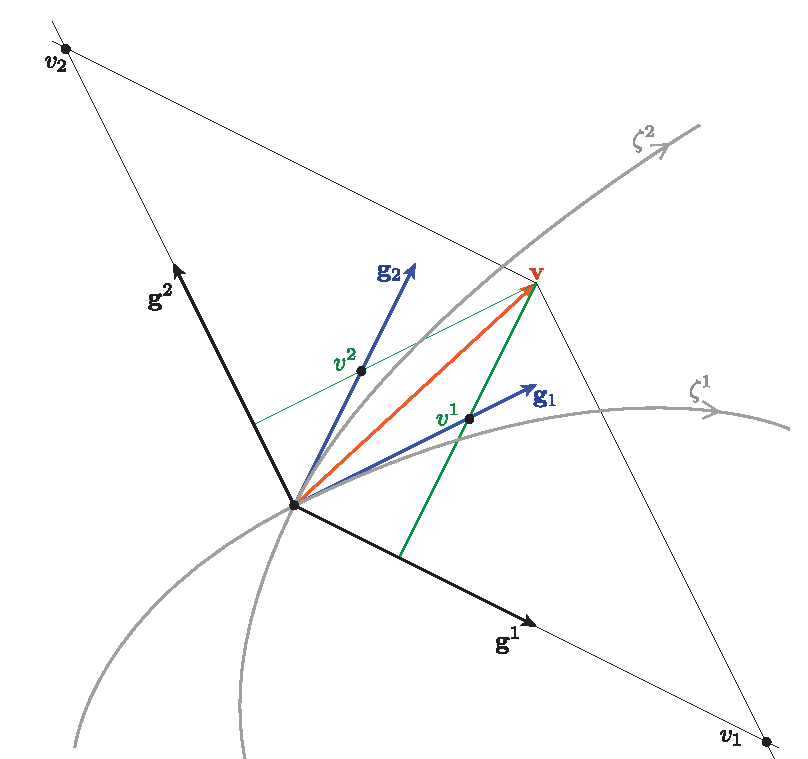
\includegraphics[scale=0.7]{figure/cinematica/covariante}
\caption{A set of non-orthogonal coordinates. The vectors of the covariant basis $\gb_1$ are tangent to the coordinate lines, while the vectors of the contravariant basis $\gb_{i}$ are such that $\gb_1\cdot \gb^2=0$ and $\gb_2\cdot\gb^1=0$. }
	\label{fig:covariante}
\end{figure}



	
	The deformation gradient can be determined as
\begin{definition}
		\begin{equation}\label{Fdy}
		\Fb=\partial_\xb \yb=(\partial_{\zeta^i} \yb)\,(\partial_\xb\zeta^i)=\hb_i\otimes\gb^i, \quad \hb_i:=\partial_{\zeta^i} \yb, \;\gb^i:=\partial_\xb\zeta^i,
	\end{equation}
\end{definition}
	where the vectors $\gb^i\in\Vr$ compose the \textit{contravariant base} in the reference placement and the vectors $\hb_i\in\Vcu$ compose the covariant base in the current placement. It is worth noticing that 
	\begin{equation}
	\partial_{\zeta^j}\zeta^i=\delta^{i}_j,
	\end{equation}
where $\delta^{i}_j$ is the Dirac delta. Therefore
	\begin{equation}
		(\partial_\xb\zeta^i)\cdot(\partial_{\zeta^j}\xb)=\delta^i_j \qquad \gb^i\cdot\gb_j={\delta}^i_j,
	\end{equation}
	where $\gb_j$ define the covariant base in the reference placement. Since
	\begin{equation}
		\Fb\gb_i=\hb_i,
	\end{equation}
	it is evident that $\Fb$ transforms the covariant base in $\Vr$ into the covariant base in $\Vcu$.
	
	In this way it is also evident that $\Fb^\top$, which has the dyadic representation
	\begin{equation}
		\Fb^\top=\gb^i\otimes\hb_i
	\end{equation}
	maps $\Vcu$ into $\Vr$. Similarly, we have that
	\begin{equation}
		\Fb^{-1}=\gb_i\otimes\hb^i,
	\end{equation}
	maps   $\Vcu$ into $\Vr$.

We can also see that $\Fb\Fb^{-1}$ and $\Fb^{-1}\Fb$ are not the same object:
\begin{equation}
\Fb\Fb^{-1}=(\hb_i\otimes\gb^i)(\gb_i\otimes\hb^i)=\hb_i\otimes\hb^i=\Ib_{\rm cur},
\end{equation}
\textit{i.e.}, the \textit{metric tensor} in the current configuration, while 
\begin{equation}
\Fb^{-1}\Fb=(\gb_i\otimes\hb^i)(\hb_i\otimes\gb^i)=\gb_i\otimes \gb^i=\Ib_{\rm ref},
\end{equation}
\textit{i.e.}, the \textit{metric tensor} in the referential configuration.

Finally, since
	\begin{equation}
		\Cb=\Fb^\top\Fb=(\gb^i\otimes\hb_i)(\hb_j\otimes\gb^j)=(\hb_i\cdot\hb_j)\gb^i\otimes\gb^j,
	\end{equation}
	\begin{equation}
		\Bb=\Fb\Fb^\top= (\hb_i\otimes\gb^i)(\gb^j\otimes\hb_j)=(\gb^i\cdot\gb^j)\hb_i\otimes\hb_j.
	\end{equation}
	we conclude that $\Cb$ is a linear transformation of $\Vr$ into itself, while $\Bb$ is  a linear transformation of $\Vcu$ into itself.



\begin{exercise}
	Given the following deformation gradient:
	\begin{equation}
		\Fb = -\frac{1}{2}(\alpha + \beta)\eb_1 \otimes \eb_1 + \frac{1}{2}(\alpha - \beta)\eb_2 \otimes \eb_2 - \frac12 (\alpha + \beta)(\eb_1 \otimes \eb_2 - \eb_2 \otimes \eb_1) + \gamma \,\eb_3 \otimes \eb_3,
	\end{equation}
	with $\alpha, \beta$, and $\gamma$ positive constants. Determine the polar decomposition of $\Fb$.
	\begin{svolgimento}
		The matrix representation of $\Fb$ is 
		\begin{equation}
			[\Fb]= \left[
			\begin{array}{ccc}
				-\dfrac{\alpha + \beta}{2} & -\dfrac{1}{2} (\alpha + \beta ) & 0 \\ [.2cm]
				\dfrac{\alpha + \beta}{2} & \dfrac{\alpha - \beta}{2} & 0 \\[.2cm]
				0 & 0 & \gamma  \\
			\end{array}
			\right]
		\end{equation}
		A simple calculation shows that the representative matrix of the right Cauchy-Green tensor $\Cb = \Fb^\top \Fb$ is
		\begin{equation}
			[\Cb]=\left[
			\begin{array}{ccc}
				\dfrac{1}{2} \left(\alpha^2 + \beta^2\right) & \dfrac{1}{2} (\alpha - \beta ) (\alpha + \beta ) & 0 \\[.2cm]
				\dfrac{1}{2} (\alpha - \beta ) (\alpha + \beta ) & \dfrac{1}{2} \left(\alpha^2 + \beta^2\right) & 0 \\[.2cm]
				0 & 0 & \gamma^2 \\
			\end{array}
			\right]
		\end{equation}
		We now determine the eigenvalues of $\Cb$, solving the characteristic polynomial
		\begin{equation}
			\det(\Cb - \lambda \Ib) = \left(\gamma^2 - \lambda \right) \left(\alpha^2 \beta^2 - \alpha^2 \lambda - \beta^2 \lambda + \lambda^2\right),
		\end{equation}
		whose solutions are
		\begin{equation}
			\lambda_1 = \alpha^2, \quad \lambda_2 = \beta^2, \quad \lambda_3 = \gamma^2.
		\end{equation}
		The corresponding eigenvectors are
		\begin{equation}
			\cb_1 = \frac{1}{\sqrt{2}}(\eb_1 + \eb_2), \quad \cb_2 = \frac{1}{\sqrt{2}}(-\eb_1 + \eb_2), \quad \cb_3 = \eb_3.
		\end{equation}
		The spectral representation of $\Cb$ is thus
		\begin{equation}
			\Cb = \alpha^2 \, \cb_1 \otimes \cb_1 + \beta^2 \, \cb_2 \otimes \cb_2 + \gamma^2 \eb_3 \otimes \eb_3,
		\end{equation}
		and therefore
		\begin{equation}
			\Ub = \alpha \, \cb_1 \otimes \cb_1 + \beta \, \cb_2 \otimes \cb_2 + \gamma \, \eb_3 \otimes \eb_3.
		\end{equation}
		The inverse of $\Ub$ is immediately found:
		\begin{equation}
			\Ub^{-1} = \frac{1}{\alpha} \, \cb_1 \otimes \cb_1 + \frac{1}{\beta} \, \cb_2 \otimes \cb_2 + \frac{1}{\gamma} \, \eb_3 \otimes \eb_3,
		\end{equation}
		or, recalling the expression for the eigenvectors,
		\begin{equation}
			\Ub^{-1} = \left[
			\begin{array}{ccc}
				\dfrac{\alpha + \beta}{2 \alpha \beta} & \dfrac{1}{2} \left(\dfrac{1}{\alpha} - \dfrac{1}{\beta}\right) & 0 \\[.2cm]
				\dfrac{1}{2} \left(\dfrac{1}{\alpha} - \dfrac{1}{\beta}\right) & \dfrac{\alpha + \beta}{2 \alpha \beta} & 0 \\[.2cm]
				0 & 0 & \dfrac{1}{\gamma} \\
			\end{array}
			\right].
		\end{equation}
		The rotation tensor has the following matrix representation:
		\begin{equation}
			[\Rb] = [\Fb][\Ub^{-1}] = \left[
			\begin{array}{ccc}
				0 & -1 & 0 \\
				1 & 0 & 0 \\
				0 & 0 & 1 \\
			\end{array}
			\right].
		\end{equation}
		The polar decomposition is therefore
		\begin{equation}
			\Fb = \Rb \Ub.
		\end{equation}
	\end{svolgimento}
\end{exercise}


\begin{exercise}
	Given the displacement field
	%Libro Capecchi
	\begin{equation}
		\ub(\xb) = \frac{3}{L}x_1^2\eb_1 + \frac{2}{L^2}x_2x_3^2\eb_2 + \frac{1}{L^2}x_1x_3^2\eb_3.
	\end{equation}
	\begin{enumerate}
		\item Determine the position of the point $P$ that before the deformation occupied the position $\xb = L\eb_1 + 2L\eb_3$.
		\item Determine the deformation $\fb(\xb)$, the deformation gradient $\Fb(\xb)$, the displacement gradient $\Hb(\xb)$, the right Cauchy-Green tensor $\Cb(\xb)$, and the Green-Saint-Venant deformation tensor $\Eb_{\rm G}(\xb)$ at point $P$.
		\item Determine if the deformation is homogeneous.
		\item Calculate the relative length change $dl/dl_0$ in the direction $\eb_1$ and the relative volume change $dv/dv_0$ at point $P$.
	\end{enumerate}
	\begin{svolgimento}
		\begin{enumerate}
			\item The deformation is easily found as
			\begin{equation}
				\fb(\xb) = \ub(\xb) + \xb = \left(x_1 + \frac{3}{L}x_1^2\right)\eb_1 + \left(x_2 + \frac{2}{L^2}x_2x_3^2\right)\eb_2 + \left(x_3 + \frac{1}{L^2}x_1x_3^2\right)\eb_3.
			\end{equation}
			Thus, the position of point $P$ after deformation is
			\begin{equation}
				\yb(P) = \fb(\xb(P)) = 2L(2\eb_1 + 3\eb_3).
			\end{equation}
			\item
			Using the definition, we have
			\begin{equation}
				\begin{aligned}
					\Fb(\xb) &= \fb{,_i} \otimes \eb_i = \left(1 + \frac{6x_1}{L}\right)\eb_1 \otimes \eb_1 + \frac{x_3^2}{L^2}\eb_3 \otimes \eb_1 + \left(1 + \frac{2x_3^2}{L^2}\right)\eb_2 \otimes \eb_2 \\
					&+ \frac{4x_2x_3}{L^2} \eb_2 \otimes \eb_3 + \left(1 + \frac{2x_1x_3}{L^2}\right)\eb_3 \otimes \eb_3.
				\end{aligned}
			\end{equation}
			Alternatively, considering the components, remembering that $F_{ij} = f_{i,j}$,\footnote{Recall that $f_{i,j}$ means $\frac{\partial f_i}{\partial x_j}$.} the representative matrix of $\Fb$ is
			\begin{equation}
				[\Fb(\xb)] = \left[\begin{matrix}
					1 + \frac{6x_1}{L} & 0 & 0 \\
					0 & 1 + \frac{2x_3^2}{L^2} & \frac{4x_2x_3}{L^2} \\
					\frac{x_3^2}{L^2} & 0 & 1 + \frac{2x_1x_3}{L^2}
				\end{matrix}\right].
			\end{equation}
			Evaluating $\Fb$ at point $P$, we get
			\begin{equation}
				\Fb(\xb(P)) = 7\eb_1 \otimes \eb_1 + 9\eb_2 \otimes \eb_2 + 4\eb_3 \otimes \eb_1 + 5\eb_3 \otimes \eb_3.
			\end{equation}
			Similarly, for $\Hb(\xb)$, once $\Fb(\xb)$ is calculated, we remember that $\Hb = \Fb - \Ib$:
			\begin{equation}
				\Hb(\xb) = \left(\frac{6x_1}{L}\right)\eb_1 \otimes \eb_1 + \frac{x_3^2}{L^2}\eb_3 \otimes \eb_1 + \left(\frac{2x_3^2}{L^2}\right)\eb_2 \otimes \eb_2 + \frac{4x_2x_3}{L^2}\eb_2 \otimes \eb_3 + \left(\frac{2x_1x_3}{L^2}\right)\eb_3 \otimes \eb_3.
			\end{equation}
			%
			Finally, the right Cauchy-Green tensor is determined as
			\begin{equation}
				\Cb(\xb(P)) = 65\eb_1 \otimes \eb_1 + 20(\eb_1 \otimes \eb_3 + \eb_3 \otimes \eb_2) + 81\eb_2 \otimes \eb_2 + 25\eb_3 \otimes \eb_3,
			\end{equation}
			and the Green-Saint-Venant tensor is
			\begin{equation}
				\Eb_{\rm G}(\xb(P)) = \frac{1}{2}(\Cb(\xb(P)) - \Ib) = \Big( 32\eb_1 \otimes \eb_1 + 10(\eb_1 \otimes \eb_3 + \eb_3 \otimes \eb_2) + 40\eb_2 \otimes \eb_2 + 12\eb_3 \otimes \eb_3 \Big).
			\end{equation}
			\item Since $\Fb(\xb)$ is not constant, the deformation is not homogeneous.
			\item The relative length change at point $P$ in the direction $\eb_1$ is
			\begin{equation}
				\frac{d\ell}{d\ell_0} = |\Fb(\xb(P)) \eb_1| = \sqrt{65},
			\end{equation}
			while the relative volume change is
			\begin{equation}
				\frac{dv}{dv_0} = \det(\Fb(\xb(P))) = 315.
			\end{equation}
		\end{enumerate}
	\end{svolgimento}
\end{exercise}

\begin{exercise}
	Let $\rb : [0,2\pi] \mapsto \Omega$ be the cylindrical helix parametrized by
	\begin{equation}
		\rb(\theta) = \cos\theta \eb_1 + \sin\theta \eb_2 + \theta \eb_3
	\end{equation}
	and let $\fb$ be the deformation
	\begin{equation}
		\fb(\xb) = x_2 \eb_1 + x_1 \eb_2 + 2x_3 \eb_3.
	\end{equation}
	\begin{enumerate}
		\item Determine the deformation gradient $\Fb(\xb)$ and the right Cauchy-Green tensor $\Cb(\xb)$.
		\item Calculate the lengths $\ell_0$ of the undeformed helix and $\ell$ of the deformed helix.
	\end{enumerate}
	
	\begin{svolgimento}
		\begin{enumerate}
			\item Using the definition, we immediately calculate
			\begin{equation}
				\Fb(\xb) = \fb{,_i}(\xb) \otimes \eb_i = \eb_2 \otimes \eb_1 + \eb_1 \otimes \eb_2 + 2\eb_3 \otimes \eb_3.
			\end{equation}  
			On the other hand, using the component representation and recalling that $F_{ij} = f_{i,j}$, we find
			\begin{equation}
				[\Fb] = \left[
				\begin{matrix}
					0 & 1 & 0 \\
					1 & 0 & 0 \\
					0 & 0 & 2
				\end{matrix}
				\right].
			\end{equation}
			Finding the Cauchy-Green tensor is straightforward:
			\begin{equation}
				\Cb = \Fb^\top \Fb = \eb_1 \otimes \eb_1 + \eb_2 \otimes \eb_2 + 4 \eb_3 \otimes \eb_3,
			\end{equation}
			or
			\begin{equation}
				[\Cb] = [\Fb^\top \Fb] = \left[
				\begin{matrix}
					1 & 0 & 0 \\
					0 & 1 & 0 \\
					0 & 0 & 4
				\end{matrix}
				\right].
			\end{equation}
			
			\item The generic point of the helix is given by $\rb(\theta)$, varying with $\theta \in [0, 2\pi]$. To find the initial length of the helix, we use the formula for calculating the length of a curve:
			\begin{equation}
				\ell_0 = \int_0^{2\pi} |\rb'(\theta)| d\theta = 2\sqrt{2} \pi.
			\end{equation}
			Due to the deformation, the generic point of the helix is mapped to
			\begin{equation}
				\yb = \fb(\rb(\theta)) = \sin\theta \eb_1 + \cos\theta \eb_2 + 2\theta \eb_3.
			\end{equation}
			The length of the deformed helix is then
			\begin{equation}
				\ell = \int_0^{2\pi} |\yb'(\theta)| d\theta = 2\sqrt{5} \pi.
			\end{equation}
		\end{enumerate}
	\end{svolgimento}
	
\end{exercise}

\begin{exercise}
Let us consider 
		the curvilinear cylindrical coordinates $(\zeta^1=\rho,\zeta^2=\varphi,\zeta^3=x_3)$; the position vector of point $x$ is then
		$$
		\xb=x-o=\rho\eb(\varphi)+x_3\eb_3, \quad \eb(\varphi):=\cos\varphi\eb_1+\sin\varphi \eb_2.
		$$
Determine the covariant and contravariant basis.

\begin{svolgimento}
			The covariant vector basis is:
		\begin{equation}
			\gb_1=\partial_{\zeta^1}\xb=\eb(\varphi), \quad \gb_2=\partial_{\zeta^2}\xb=\rho\eb'(\varphi), \quad \gb_3=\partial_{\zeta^3}\xb=\eb_3.
		\end{equation}
		To determine the contravariant vector basis, we notice that
		$$
		x_1=\xb\cdot\eb_1=\rho\cos\varphi, \quad x_2=\xb\cdot\eb_2=\rho\sin\varphi;
		$$
		since $\rho^2=x_1^2+x_2^2$, and $\tan\varphi=\frac{x_2}{x_1}$, we get
		$$
		\gb^1=\partial_\xb\zeta^1=\nabla\rho=\frac{x_1}{\rho}\eb_1+\frac{x_2}{\rho}\eb_2=\eb(\varphi), \quad 
		\gb^2=\partial_\xb\zeta^2=\nabla\varphi=\frac{1}{\rho}\eb'(\varphi).
		$$
\end{svolgimento}
	
\end{exercise}

\section{Motion velocity, velocity gradient, stretching, and spin}
On introducing the time variable $t\in\Ro^+$, we use the following notation:\\
\noindent for a \textit{motion},
\begin{equation}
	(\xb,t)\mapsto \yb=\fb(\xb,t)=:\fb_t(\xb);
\end{equation} 
for the deformation gradient and the \textit{motion velocity} $\vb$
\begin{equation}
	\Fb=\partial_\xb \yb, \qquad \vb=\partial_t \yb.
\end{equation}

Let us consider a \textit{referential} field $\varphi=\phi(\xb,t)$; we will use the notation
\begin{equation}
	\nabla\varphi=\partial_\xb\varphi, \qquad \dot{\varphi}=\partial_t\varphi.
\end{equation}
Some care is needed if the current counterpart of $\varphi$ is considered:
\begin{equation}
	\varphi=\widehat{\varphi}(\yb,t):=\phi\big( \fb_t^{-1}(\yb),t  \big).
\end{equation}
In this case we have
\begin{equation}
	\dot{\varphi}=(\partial_\yb\phi)\partial_t \yb+\partial_t\varphi=(\partial_\yb\varphi)\vb+\partial_t\varphi.
\end{equation}
In order to distinguish the spatial derivative with respect to current point $\yb$, we introduce the following notation
\begin{equation}
	\grad\varphi=\partial_\yb\varphi.
\end{equation}
Then, we have
\begin{equation}
	\dot\varphi=(\grad\varphi)\,\vb+\partial_t\varphi.
\end{equation}
For any field $\varphi$ that is given both a referential and current description, the relation
\begin{definition}
\begin{equation}
	\nabla\varphi=(\grad \varphi)\Fb
\end{equation}
\end{definition}
holds true, as proved by the following sequence of equalities:
\begin{equation}
	\nabla\varphi=\partial_\xb\varphi=(\partial_\yb\varphi)(\partial_\xb \yb)=(\grad \varphi)\Fb.
\end{equation}


We introduce the \textit{velocity gradient} $\Lb$:
\begin{equation}
	\Lb(\yb,t):=\partial_\yb\vb=\grad\vb.
\end{equation}
Now, we have that
\begin{equation}
	\dot{\Fb}=\partial_t(\partial_\xb \yb)=\partial_\xb(\partial_t \yb)=\partial_\xb\vb=(\partial_\yb\vb)(\partial_\xb \yb)=\Lb\Fb,
\end{equation}
and then
\begin{definition}
\begin{equation}
	\Lb=\dot\Fb\Fb^{-1}.
\end{equation}
\end{definition}

%The gradient velocity $\Lb$ tells how velocity varies from point to point in the current configuration: $\dot\Fb$ tells  how the deformation is changing over time at a fixed material point, but we want to know the current rate of change of the velocity field; to do that, we must move from the referential description to the current description, through $\Fb^{-1}$.

It accounts for both stretching and rotation of material elements.


The symmetric and skew-symmetric parts of $\Lb$
\begin{equation}
	\Db=\frac 12 (\Lb+\Lb^\top), \quad \Wb=\frac 12 (\Lb-\Lb^\top)
\end{equation}
are called \textit{stretching tensor} and \textit{spin tensor}; the former is a measure of the \textit{strain rate}, while the latter is a measure of the \textit{motion vorticity}.


%\begin{exercise}
%	A deformation of the form
%	\begin{equation}
%		\begin{aligned}
%			& y_1=x_1+\gamma x_2\\
%			& y_2=x_2,\\
%			& y_3=x_3
%			\end{aligned}
%		\end{equation}
%	is called \emph{pure shear}. For this deformation compute:
%	\begin{enumerate}
%			\item the matrices of $\Fb,\Cb$ and $\Bb$;
%%			\item the list of principal invariants of $\Cb$;\footnote{We recall that, for a second order tensor $\Ab$, the principal invariants are:
%%				$$
%%				I_1=\tr{\Ab}, \quad I_2=\frac{1}{2}\big((\tr{\Ab})^2-\tr{\Ab^2}  \big), \quad I_3=\det\Ab.
%%				$$
%%			They are the coefficients of the  characteristic polynomial $\det(\Ab-\lambda\Ib)$, whose solutions are the eingevalues of $\Ab$.
%%					\item the principal stretches, i.e., the eigenvalues of $\Ub$ or $\Vb$.
%	\end{enumerate}
%\end{exercise}

\begin{exercise}
	Show that a deformation is  \emph{isochoric} (i.e. volume preserving) if $\det\Cb=1$.
\end{exercise}


%\begin{exercise}
%Show that a deformation is rigid if and only if the list of invariants of $\Cb$ is $(3,3,1)$.
%\end{exercise}



\begin{exercise}
	The deformation of a two-dimensional continuum is given as
	$$
	y_1=4-2x_1-x_2; \quad y_2=2+\frac{2}{3}x_1-\frac{1}{2}x_2.
	$$
	\begin{enumerate}
			\item Calculate the deformation gradient tensor $\Fb$, the right Cauchy-Green strain tensor $\Cb$ and the left Cauchy-Green strain tensor $\Bb$.
			\item Calculate the stretch undergone by a unit material vector $\ab_0=\frac{3}{5}\eb_1+\frac{4}{5}\eb_2$ as a result of the deformation.
			\item Demonstrate whether or not the deformation is isochoric. 
		\end{enumerate}
\end{exercise}

\begin{exercise}
	A deformation of the form
$$
	\begin{aligned}
		& y_1=f_1(x_1,x_2)\\
		& y_2=f_2(x_1,x_2),\\
		& y_3=x_3
		\end{aligned}
$$
	is called \textit{plane strain}. Show that for such a deformation the principal stretch $\lambda_3$ (in $x_3$ direction) is unity. Show further that the deformation is isochoric if and only if the other principal stretches, $\lambda_\alpha$ and $\lambda_\beta$ satisfy
	$$
	\lambda_\alpha=\frac{1}{\lambda_\beta}.
	$$
\end{exercise}
%
%
%\begin{exercise}
%	Let 
%	$$
%	\varepsilon=|\Fb-\Ib|=|\nabla\ub|
%	$$
%	a smallness parameter, so that $\Fb(\varepsilon)=\Ib+\varepsilon\nabla\ub$.
%	\begin{enumerate}
	%		\item compute the linear approximation about $\varepsilon=0$ of the Green--St. Venant tensor $\Eb$ and show that
	%		$$
	%		\Eb\simeq\Gb, \qquad \Gb:=\sym\nabla\ub,
	%		$$
	%	i.e., the  strain measure adopted in linear elasticity;
	%	\item show that
	%$$
	%\delta l(\eb)\simeq\eb\cdot\Gb\eb;
	%$$
	%\item show that
	%$$
	%\delta a(\nb_{\rm ref})\simeq\Gb\cdot(\Ib-\nb_{\rm ref}\otimes\nb_{\rm ref})
	%$$
	%\item show that
	%$$
	%\delta v\simeq\Gb\cdot\Ib=\tr{\Eb}.\footnote{To this end, it is useful to recall a formula known to Euler:
		%	$$
		%	\partial_{\Ab}(\det\Ab)=\Ab^*.
		%	$$}
	%$$
	%
	%	\end{enumerate}
%\end{exercise}
%
\begin{exercise}
	Prove that
	$$
	\dot{\Cb}=2\Fb^\top\Db\Fb.
	$$
\end{exercise}


\chapter{Infinitesimal Theory}\label{inf}

From equation \eqref{dl}, it follows that if the deformation gradient is close to the identity, then the variations in length are small. We can thus introduce a smallness parameter, given by
\begin{equation}
	\varepsilon\coloneqq\sup_{\xb\in\Omega}|\Fb(\xb)-\Ib|,
\end{equation}
which measures the greatest distance between \(\Fb\) and the identity. Given the definition of displacement gradient and equation \eqref{HFI}, the parameter can be rewritten as
\begin{equation}\label{eps}
	\varepsilon=\sup_{\xb\in\Omega}|\Hb(\xb)|.
\end{equation}

We now want to consider a theory, called the \textit{infinitesimal theory}, obtained by neglecting infinitesimals of order higher than the first in \(\varepsilon\).


\section{The Infinitesimal Strain Tensor}

First, let's see what the deformation measures are in the infinitesimal theory. We observe that we can write the deformation gradient as
\begin{equation}
	\Fb(\xb)=\Ib +\varepsilon(\xb) \widetilde{\Hb}(\xb), \qquad \varepsilon(\xb)\coloneqq |\Hb(\xb)|, \quad \widetilde{\Hb}(\xb)\coloneqq \frac{\Hb(\xb)}{|\Hb(\xb)|}.
\end{equation}
Given equation \eqref{eps}, certainly
\begin{equation}
	\varepsilon(\xb)\leq \varepsilon \qquad \forall \xb\in \Omega
\end{equation}
and thus we are allowed to neglect terms of order \(\varepsilon^2(\xb)\). Neglecting these terms, the right Cauchy-Green tensor then becomes
\begin{equation}\label{Cap}
	\begin{aligned}
		\Cb(\xb)=	\mathbf{F}^\top(\mathbf{x})\mathbf{F}(\mathbf{x})& =\mathbf{I+H^\top(x)+H(x)}+\frac12\Hb^\top(\xb)\Hb(\xb) \\
		&=\mathbf{I}+\varepsilon(\mathbf{x})\widetilde{\mathbf{H}}^\top(\mathbf{x})+\varepsilon(\mathbf{x})\widetilde{\mathbf{H}}(\mathbf{x})+\frac12\varepsilon^2(\mathbf{x})\widetilde{\mathbf{H}}^\top(\mathbf{x})\widetilde{\mathbf{H}}(\mathbf{x}) \\
		&=\mathbf{I}+\varepsilon(\mathbf{x})\widetilde{\mathbf{H}}^\top(\mathbf{x})+\varepsilon(\mathbf{x})\widetilde{\mathbf{H}}(\mathbf{x}) \\
		&=\mathbf{I+H^\top(x)+H(x)}.
	\end{aligned}
\end{equation}
In the following, we will avoid introducing the parameter \(\varepsilon\) and neglect terms that are superlinear in \(\Hb\).

The Green-Saint-Venant deformation measure thus becomes
\begin{equation}
	\Eb_{\rm G}(\xb)=\frac{1}{2}(\Cb(\xb)-\Ib)=\frac{1}{2}\left(\mathbf{H(x)+H^\top(x)}\right).
\end{equation}

The tensor
\begin{definition}
	\begin{equation}\label{simgrad}
		\Eb(\xb)\coloneqq\sym \Hb(\xb)
	\end{equation}
\end{definition}
is called the \textit{infinitesimal strain tensor}, which will be used to completely characterize the metric variations in infinitesimal theory.

\section{The Infinitesimal Rotation Tensor}

Like any second-order tensor, the displacement gradient can be decomposed into its symmetric and skew-symmetric parts:
\begin{equation}
	\Hb=\sym \Hb+\skw \Hb.
\end{equation}
We have already defined the infinitesimal deformation tensor \(\Eb=\sym \Hb\); now we show that the skew-symmetric part
\begin{definition}
	\begin{equation}
		\Wb\coloneqq\skw \Hb
	\end{equation}
\end{definition}
represents an infinitesimal rigid rotation. To show this, we approximate the relation
\begin{equation}
	\Rb=\Fb\Ub^{-1}
\end{equation}
to see the form of an infinitesimal rotation. Neglecting superlinear terms in \(\Hb\), from \eqref{Cap} we have
\begin{equation}
	\Ub^2=\Cb=\Ib+2\Eb.
\end{equation}
On the other hand, the following chain of equalities holds:
\begin{equation}
	(\Ib+\Eb)^2=(\Ib+\Eb)(\Ib+\Eb)=\Ib+2\Eb=\Ub^2,
\end{equation}
from which we can deduce that
\begin{equation}
	\Ub=\Ib+\Eb.
\end{equation}
Now that we have the approximation for \(\Ub\), we need to find the one for \(\Ub^{-1}\). Since
\begin{equation}
	(\Ib+\Eb)(\Ib-\Eb)=\Ib,
\end{equation}
we can conclude that
\begin{equation}
	\Ub^{-1}=\Ib-\Eb.
\end{equation}
We are now ready to determine the form that a rotation \(\Rb\) takes when superlinear terms in \(\Hb\) (i.e., small deformations) are neglected:
\begin{equation}
	\Rb=\Fb\Ub^{-1}=(\Ib+\Hb)(\Ib-\Eb)=\Ib-\Eb+\Hb=\Ib+\Wb.
\end{equation}
Thus, we conclude that the rotation of a point \(\xb\) around \(\xb_0\) has the following representation in infinitesimal theory:
\begin{equation}
	\Rb(\xb-\xb_0)=(\xb-\xb_0)+\Wb(\xb-\xb_0).
\end{equation}
Since, in a rigid displacement \(\nabla \ub=\Fb-\Ib=\Rb-\Ib=\Wb\), we obtain the following representation of the \textit{infinitesimal rigid displacement} field:
\begin{definition}
	\begin{equation}\label{urig}
		\ub_{\rm rig}(\xb)=\ub(\xb_0)+\Wb (\xb-\xb_0).
	\end{equation}
\end{definition}
Since an skew-symmetric tensor \(\Wb\) can be associated with a vector \(\wb\), according to the following correspondence
\begin{equation}
	\Wb \ab=\wb \times \ab \quad \forall \ab\in \Vc,
\end{equation}
\eqref{urig} can be equivalently rewritten as
\begin{definition}
	\begin{equation}\label{urig}
		\ub_{\rm rig}(\xb)=\ub(\xb_0)+\wb \times(\xb-\xb_0).
	\end{equation}
\end{definition}
The vector \(\wb\) is called the \textit{axial} vector of \(\Wb\). Its unit vector \(\wb/|\wb|\) represents the axis of rotation, while its magnitude gives the (infinitesimal) angle of rotation.

\begin{remark}\label{skvec}
	Let us choose a Cartesian basis \(\{\eb_i\}\) and represent the tensor \(\Wb\in\Skw\) in matrix form:
	\begin{equation}
		[\Wb]=\left[\begin{array}{ccc}0&-\gamma&\beta\\\gamma&0&-\alpha\\-\beta&\alpha&0\end{array}\right].
	\end{equation}
	A simple calculation shows that the axial vector of \(\Wb\) is then
	\begin{equation}
		\wb=\alpha\eb_1+\beta\eb_2+\gamma\eb_3.
	\end{equation}
\end{remark}

Both \(\Rb\) and \(\Wb\) are constant tensors, having considered a homogeneous deformation. However, the general deformation \(\fb(\xb)\) of a point \(\xb\) can be expanded in a series around another point \(\xb_0\):
\begin{equation}
	\fb(\xb)=\fb(\xb_0)+\Fb(\xb_0)(\xb-\xb_0)+o(|\xb-\xb_0|).
\end{equation}
This means that in the neighborhood of a point \(\xb\), to an error of the order \(o(|\xb-\xb_0|)\), any deformation behaves as if it were homogeneous. This justifies the following terminology: let
\begin{equation}
	\Fb(\xb)=\Rb(\xb)\Ub(\xb)
\end{equation}
be the \textit{local} polar decomposition for \(\Fb(\xb)\); then \(\Rb(\xb)\) is the \textit{local} rotation tensor and \(\Ub(\xb)\) the \textit{local} Cauchy-Green tensor. \(\Rb(\xb)\) is a measure of the local rigid rotation of points close to \(\xb\), while \(\Ub(\xb)\) is a measure of the deformation around \(\xb\).

Similarly, in infinitesimal theory, we can say that
\begin{equation}
	\Hb(\xb)=\Eb(\xb)+\Wb(\xb)
\end{equation}
is the \textit{local} decomposition of the displacement gradient; the tensor \(\Eb(\xb)\) is the \textit{local} infinitesimal deformation tensor, and \(\Wb(\xb)\) is the \textit{local} infinitesimal rotation tensor. \(\Eb(\xb)\) is a measure of the infinitesimal deformation around \(\xb\), and \(\Wb(\xb)\) is a measure of the local rigid infinitesimal rotation of points close to \(\xb\).



\section{Geometric Changes}

\subsection{Change in Length}
Recalling \eqref{dl}, the ratio between the deformed and undeformed length of an infinitesimal segment in the direction $\tb$, neglecting the superlinear terms in $\Hb$, can be calculated as
\begin{equation}
	\frac{d\ell}{d\ell_0}=|\Fb\tb|=\sqrt{\Cb\tb\cdot\tb}=\sqrt{(\Ib+2\Eb)\tb\cdot\tb}=(\Ib+\Eb)\tb\cdot\tb=1+\Eb\tb\cdot\tb.
\end{equation}
Therefore, in infinitesimal theory, the specific variation in length in the direction $\tb$ is
\begin{definition}
	\begin{equation}\label{Ett}
		\frac{d\ell-d\ell_0}{d\ell_0}=\frac{d\ell}{d\ell_0}-1=\Eb\tb\cdot\tb.
	\end{equation}
\end{definition}

\subsection{Change in Volume}
Without loss of generality, consider a volume element generated by the base vectors, so that $dv_0=\eb_1\times\eb_2\cdot\eb_3=1$. The deformed volume will then be
\begin{equation}
	\begin{aligned}
		dv&=\Fb\eb_1\times\Fb\eb_2\cdot\Fb\eb_3=\det\mathbf{F}=\det(\Ib+\Hb)=(\Ib+\Hb)\eb_1\times(\Ib+\Hb)\eb_2\cdot(\Ib+\Hb)\eb_3\\
		&=\mathbf{e}_{1}\times\mathbf{e}_{2}\cdot\mathbf{e}_{3}+\mathbf{H}\mathbf{e}_{1}\times\mathbf{e}_{2}\cdot\mathbf{e}_{3}+\mathbf{e}_{1}\times\mathbf{H}\mathbf{e}_{2}\cdot\mathbf{e}_{3}+\mathbf{e}_{1}\times\mathbf{e}_{2}\cdot\mathbf{H}\mathbf{e}_{3}\\
		&=1+\mathbf{e}_{2}\times\mathbf{e}_{3}\cdot\mathbf{H}\mathbf{e}_{1}+\mathbf{e}_{3}\times\mathbf{e}_{1}\cdot\mathbf{H}\mathbf{e}_{2}+\mathbf{e}_{1}\times\mathbf{e}_{2}\cdot\mathbf{H}\mathbf{e}_{3}\\
		&=1+\mathbf{H}\mathbf{e}_{1}\cdot\mathbf{e}_{1}+\mathbf{H}\mathbf{e}_{2}\cdot\mathbf{e}_{2}+\mathbf{H}\mathbf{e}_{3}\cdot\mathbf{e}_{3}=1+\operatorname{tr}\mathbf{H}=1+\operatorname{tr}\mathbf{E},
	\end{aligned}
\end{equation}
since $\operatorname{tr}\Wb=0$. It follows that, in infinitesimal theory, the volume variation is
\begin{equation}
	\frac{dv}{dv_0}=1+\operatorname{tr}\Eb,
\end{equation}
that is,
\begin{definition}
	\begin{equation}\label{trE}
		\frac{dv-dv_0}{dv_0}=\operatorname{tr}\mathbf{E}.
	\end{equation}
\end{definition}

\subsection{Change in Area}
Without loss of generality, suppose we consider an area generated by the vectors $\eb_1$ and $\eb_2$, whose reference normal is $\nb_{\rm ref}=\eb_1\times\eb_2=\eb_3$. The initial infinitesimal area is $da_0=|\nb_{\rm ref}|=1$. Neglecting superlinear terms in $\Hb$, the deformed area is
\begin{equation}
	\begin{aligned}
		da&=|\Fb\eb_1\times\Fb\eb_2|=|(\Ib+\Hb)\eb_1\times(\Ib+\Hb)\eb_2|\\
		&=\sqrt{1+2\eb_3\cdot(\eb_1\times\Hb\eb_2+\Hb\eb_1\times\eb_2)}=\sqrt{1+2(\Hb\eb_1\cdot\eb_1+\Hb\eb_2\cdot\eb_2)}\\
		&=1+E_{11}+E_{22}=1+(\Ib-\eb_3\otimes\eb_3)\cdot\Eb.
	\end{aligned}
\end{equation}
Thus, we conclude that, if $\nb_{\rm ref}$ is the reference normal to the surface, then
\begin{definition}
	\begin{equation}\label{da}
		\frac{da-da_0}{da_0}=\frac{da}{da_0}-1=(\Ib-\nb_{\rm ref}\otimes\nb_{\rm ref})\cdot\Eb,
	\end{equation}
\end{definition}
that is, the specific variation in area is equal to the trace of the strain tensor restricted to the plane in which the considered area lies.

\subsection{Change in Angle}
Consider two orthogonal vectors $\eb_{1}$ and $\eb_2$ passing through the same point. The initial angle is $\alpha_0=\pi/2$, while after deformation,
\begin{equation}
	\alpha=\arccos\left(\frac{\mathbf{F^{\top}Fe}_1\cdot\mathbf{e}_2}{|\mathbf{F^{\top}Fe}_1\cdot\mathbf{e}_1|^{1/2}|\mathbf{F^{\top}Fe}_2\cdot\mathbf{e}_2|^{1/2}}\right).
\end{equation}
Since
\begin{equation}
	\mathbf{F^{\top}Fe}_1\cdot\mathbf{e}_2=(\mathbf{I}+2\mathbf{E})\mathbf{e}_1\cdot\mathbf{e}_2=2\mathbf{Ee}_1\cdot\mathbf{e}_2
\end{equation}
and 
\begin{equation}
	\mathbf{|F^{\top}Fe}_1\cdot \eb_1|^{1/2}=\mathbf{|(I+2E)e}_1\cdot \eb_1|^{1/2}=(1+2\Eb\eb_1\cdot \eb_2)^{1/2}=1+\Eb\eb_1\cdot \eb_1
\end{equation}
we get
\begin{equation}
	\begin{aligned}
		\cos\alpha & =\frac{2\mathbf{Ee}_1\cdot\mathbf{e}_2}{(1+\mathbf{Ee}_1\cdot\mathbf{e}_1)(1+\mathbf{Ee}_2\cdot\mathbf{e}_2)}=\frac{2\mathbf{Ee}_1\cdot\mathbf{e}_2}{1+\mathbf{Ee}_1\cdot\eb_1+\mathbf{Ee}_2\cdot\eb_2}  \\
		&=\frac{2\mathbf{Ee}_1\cdot\eb_2}{1+\mathbf{Ee}_1\cdot\eb_1+\mathbf{Ee}_2\cdot\eb_2}\frac{1-\mathbf{Ee}_1\cdot\eb_1-\mathbf{Ee}_2\cdot\eb_2}{1-\mathbf{Ee}_1\cdot\eb_1-\mathbf{Ee}_2\cdot\eb_2} \\
		&=2\mathbf{Ee}_1\cdot\eb_2(1-\mathbf{Ee}_1\cdot\eb_1-\mathbf{Ee}_2\cdot\eb_2) \\
		&=2\mathbf{Ee}_1\cdot\eb_2.
	\end{aligned}
\end{equation}
We now calculate the variation in angle
\begin{equation}
	\delta\alpha=\alpha-\alpha_0=\alpha-\frac{\pi}{2}.
\end{equation}
Since
\begin{equation}
	\sin(\delta\alpha)=\sin(\frac\pi2-\alpha)=\cos\alpha,
\end{equation}
we get
\begin{equation}
	\begin{aligned}\delta\alpha&=\arcsin(\cos\alpha)=\arcsin(2\mathbf{Ee}_1\cdot\mathbf{e}_2)=2\mathbf{Ee}_1\cdot\mathbf{e}_2,\end{aligned}
\end{equation}
which is obtained using the Taylor series expansion of the arcsine: $\arcsin x=x+o(x)$ as $x\to 0$, and therefore
\begin{definition}
	\begin{equation}\label{E12}
		\begin{aligned}\delta\alpha=2\mathbf{Ee}_1\cdot\mathbf{e}_2,\end{aligned}
	\end{equation}
\end{definition}

\section{Components of the Infinitesimal Strain Tensor}
Given a Cartesian basis $\{\eb_i\}$, the infinitesimal strain tensor can be represented in matrix form as follows:
\begin{equation}
	[\Eb]=\begin{bmatrix}E_{11}&E_{12}&E_{13}\\E_{21}&E_{22}&E_{23}\\E_{31}&E_{32}&E_{33}\end{bmatrix}=\begin{bmatrix}E_{11}&E_{12}&E_{13}\\&E_{22}&E_{23}\\\mathrm{sym}&&E_{33}\end{bmatrix}.
\end{equation}

The interpretation of $E_{11}$ is immediate, recalling \eqref{Ett}:
\begin{equation}
	E_{11}=\Eb\eb_1\cdot\eb_1=\frac{d\ell-d\ell_0}{d\ell_0},
\end{equation}
that is, it represents the specific elongation along the direction $\eb_1$. An analogous interpretation can be given for all the diagonal components.

To interpret $E_{12}$, we need to refer to \eqref{E12}: 
\begin{equation}
	E_{12}=\Eb\eb_1\cdot\eb_2=\frac{\delta\alpha}{2},
\end{equation}
that is, it represents half the shear angle between the directions $\eb_1$ and $\eb_2$. A similar interpretation can be given for $E_{13}$ and $E_{23}$.

We also observe that $\operatorname{tr}\Eb=E_{11}+E_{22}+E_{33}$, as per \eqref{trE}, represents the specific variation in an infinitesimal volume generated by the three base vectors. Finally, in light of \eqref{da}, the sum $E_{11}+E_{22}$ represents the specific variation in area in the plane generated by $\eb_1$ and $\eb_2$; a similar interpretation applies to the sum of any pair of elements from the main diagonal.

\section{Elementary Deformations}
In this section, we analyze some significant homogeneous deformations.

\subsubsection{Uniform Extension}
In a uniform extension of $\varepsilon$ in the direction $\nb$ ($|\nb|=1$), the displacement field is given by
\begin{equation}
	\mathbf{u}(\mathbf{x})=\varepsilon\,\mathbf{n}\otimes\mathbf{n}(\mathbf{x}-\mathbf{x}_{0}).
\end{equation}
The generic point $\mathbf{x}$ thus moves in the direction of $\nb$, linearly increasing as $\mathbf{x}$ moves away from the fixed point $\mathbf{x}_0$.

\begin{center}
	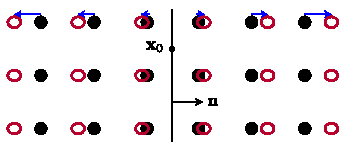
\includegraphics[scale=1.3]{figure/cinematica/estensione}
\end{center}

In this case, 
\begin{equation}
	\nabla\mathbf{u}=\varepsilon\,\mathbf{n}\otimes\mathbf{n}=\mathbf{E}.
\end{equation}
Since
\begin{equation}
	\varepsilon=\mathbf{E}\mathbf{n}\cdot\mathbf{n},
\end{equation}
the constant $\varepsilon$ represents the specific elongation in the direction of $\nb$. 

If $\mathbf{m}$ is a vector orthogonal to $\nb$, since $\mathbf{E}\mathbf{n} \cdot\mathbf{m}=0$, the angle between a fiber directed as $\nb$ and one as $\mathbf{m}$ does not change. Moreover, since $\mathbf{E}\mathbf{m} \cdot\mathbf{m}=0$, there is no variation in length in the direction of $\mathbf{m}$.

\subsubsection{Uniform Dilation}
In a dilation of $\kappa$ around $\mathbf{x}_0$, the displacement field is
\begin{equation}
	\mathbf{u}(\mathbf{x})=\kappa(\mathbf{x}-\mathbf{x}_0).
\end{equation}
All points thus move in the radial direction $\mathbf{x} -\mathbf{x}_0$, by an amount that increases linearly as one moves away from $\mathbf{x}_0$.

\begin{center}
	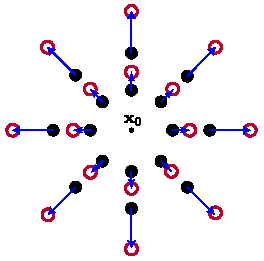
\includegraphics[scale=1.3]{figure/cinematica/dilatazione}
\end{center}

In this case,
\begin{equation}
	\nabla\mathbf{u}=\kappa \mathbf{I}=\mathbf{E}.
\end{equation}
A fiber in any direction $\mathbf{t}$ has a specific elongation
\begin{equation}
	\mathbf{E}\mathbf{t}\cdot\mathbf{t}=\kappa.
\end{equation}
The specific change in volume is
\begin{equation}
	\frac{dv-dv_0}{dv}=\operatorname{tr}\mathbf{E}=3\kappa.
\end{equation}

\subsubsection{Shear}
Consider a point $\mathbf{x}_0$ and two mutually orthogonal unit vectors $\mathbf{n}$ and $\mathbf{m}$. In a shear along $\mathbf{n}$ and $\mathbf{m}$, the displacement of a point $\mathbf{x}$ is directed as $\mathbf{m}$ and its magnitude is proportional to the distance between $\mathbf{x}$ and the plane normal to $\mathbf{n}$ passing through $\mathbf{x}_0$:
\begin{equation}
	\mathbf{u}(\mathbf{x})=\gamma\big( (\mathbf{x}-\mathbf{x}_0)\cdot\mathbf{n} \big)\mathbf{m}=\gamma \mathbf{m}\otimes\mathbf{n} (\mathbf{x} -\mathbf{x}_0).
\end{equation}

\begin{center}
	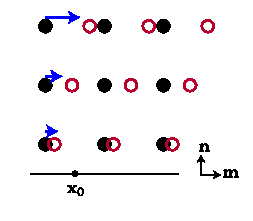
\includegraphics[scale=1.3]{figure/cinematica/scorrimento}
\end{center}

Since $\nabla\mathbf{u}=\gamma \mathbf{m} \otimes \mathbf{n}$, we deduce that
\begin{equation}
	\mathbf{E}=\frac{\gamma}{2}(\mathbf{m} \otimes \mathbf{n} +\mathbf{n} \otimes \mathbf{m}), \qquad \mathbf{W}=\frac{\gamma}{2}(\mathbf{m} \otimes \mathbf{n}-\mathbf{m} \otimes \mathbf{n}).
\end{equation}
Using \eqref{E12}, we immediately deduce that
\begin{equation}
	\frac{\delta\alpha}{2}=\mathbf{E} \mathbf{m} \cdot\mathbf{n}=\frac{\gamma}{2},
\end{equation}
and thus the shear coefficient $\gamma$ is equal to the change in angle between $\mathbf{m}$ and $\mathbf{n}$. For convenience, let us fix $\mathbf{x}_0=\mathbf{0}$, $\mathbf{m} =\mathbf{e}_1$ and $\mathbf{n}=\mathbf{e}_2$. Then, the representative matrices for $\mathbf{E}$ and $\mathbf{W}$ are:
\begin{equation}
	[\mathbf{E}(\mathbf{u})]=\frac{\gamma}{2}\begin{bmatrix}0&1&0\\1&0&0\\0&0&0\end{bmatrix}\quad\mathrm{and}\quad[\mathbf{W}(\mathbf{u})]=\frac{\gamma}{2}\begin{bmatrix}0&1&0\\-1&0&0\\0&0&0\end{bmatrix}.
\end{equation}
Since $\mathbf{u} (\mathbf{x})=\mathbf{E} \mathbf{x} +\mathbf{W} \mathbf{x}$, we conclude that
\begin{equation}
	\mathbf{u}(\mathbf{x})=\underbrace{\frac{\gamma}{2}(x_2 \mathbf{e}_1+x_1 \mathbf{e}_2)}_{\text{pure shear}} +\underbrace{ \frac{\gamma}{2}(x_2 \mathbf{e}_1-x_1 \mathbf{e}_2)}_{\text{infinitesimal rotation}}.
\end{equation}
Thus, the total displacement can be viewed as the sum of pure shear (given by $\mathbf{E} \mathbf{x}$) and an infinitesimal rotation (given by $\mathbf{W} \mathbf{x}$).  

\begin{center}
	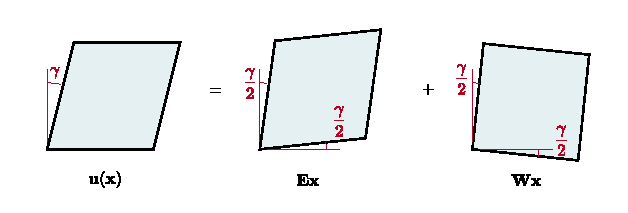
\includegraphics[scale=1.3]{figure/cinematica/scorrimento1}
\end{center}

In light of observation \ref{skvec}, the axis of $\mathbf{W}$ is
\begin{equation}
	\mathbf{w} =-\frac{\gamma}{2}\, \mathbf{e}_3.
\end{equation}
Thus, it is a rotation around the axis $\mathbf{e}_3$, by an angle $\gamma/2$; the negative sign indicates that the rotation is clockwise.

\begin{exercise}
	Given the displacement field
	\begin{equation}
		\mathbf{u}(\mathbf{x})=(\alpha_1 x_1x_2+\alpha_2 x_2)\mathbf{e}_1+(\beta_1 x_2+\beta_2 x_1)\mathbf{e}_2, \qquad \alpha_1, \alpha_2, \beta_1, \beta_2\in \mathbb{R},
	\end{equation}
	determine:
	\begin{enumerate}
		\item The deformed boundary of a square with side $L$ and two sides along the $x_1, x_2$ axes;
		\item 	The infinitesimal strain tensor and the infinitesimal rotation tensor;
		\item The final configuration and the change in length (using infinitesimal theory) of the diagonal inclined at $\pi/4$ with respect to $x_1$;
		\item The change in area (using infinitesimal theory) of the square introduced in point a).
	\end{enumerate}
	
	\begin{svolgimento}
		\begin{enumerate}
			\item Referring to the notation in the figure,
			\begin{center}
				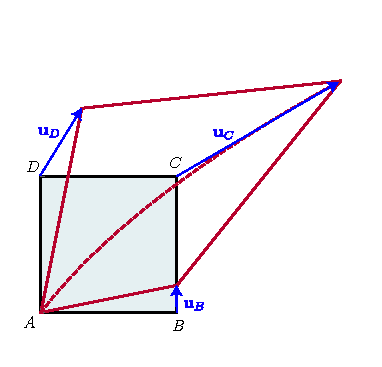
\includegraphics[scale=1]{figure/cinematica/esempio3d_1}
			\end{center}
			we can immediately calculate the displacement of the vertices:
			\begin{equation}
				\mathbf{u}_A=\mathbf{0}, \qquad \mathbf{u}_B=\beta_2 L \mathbf{e}_2, \qquad \mathbf{u}_C=(\alpha_1^2L+\alpha_2L)\mathbf{e}_1+(\beta_1+\beta_2)L\mathbf{e}_2, \qquad \mathbf{u}_D=\alpha_2L \mathbf{e}_1+\beta_1 L \mathbf{e}_2.
			\end{equation}
			The points on the side  $AB=\{ \mathbf{x}\in \mathcal{V} \,:\, \mathbf{x} =x_1\mathbf{e}_1, 0<x_1<L\}$ undergo the deformation
			\begin{equation}
				\mathbf{f}(\mathbf{x})=x_1\mathbf{e}_1+(x_2+\beta_2 x_1)\mathbf{e}_2,
			\end{equation}
			and thus the side $AB$ deforms into an inclined line at an angle given by
			\begin{equation}
				\delta x_2=\beta_2 x_1.
			\end{equation}
			\item The strain tensor is computed in the usual manner:
			\begin{equation}
				\mathbf{E}=\frac{1}{2}\left(\nabla \mathbf{u}+ (\nabla \mathbf{u})^{\top} \right)=
				\frac{1}{2}\begin{bmatrix} \alpha_1 x_2+ \alpha_2 & \alpha_1 x_1 +\beta_1 & 0\\
					\alpha_1 x_1+\beta_1 & \beta_2 & 0\\
					0 & 0 & 0 \end{bmatrix}.
			\end{equation}
		\end{enumerate}
	\end{svolgimento}
\end{exercise}

\begin{exercise}
	A \textit{strain gauge rosette} is an electromechanical device that measures the percentage elongation in three directions. By mounting such a device on the surface of a structure, it is possible to determine the axial strains in certain directions. A schematic representation of a rosette is shown in the figure. Assume that in an experiment, the specific elongations in the directions defined by the unit vectors $\ab$, $\bb$, and $\cb$ were measured, resulting in $\varepsilon_a$, $\varepsilon_b$, and $\varepsilon_c$. Using infinitesimal theory, determine the components of the specific elongation in the directions $\eb_1$ and $\eb_2$ and the angle change between $\eb_1$ and $\eb_2$.
	%
	\begin{center}
		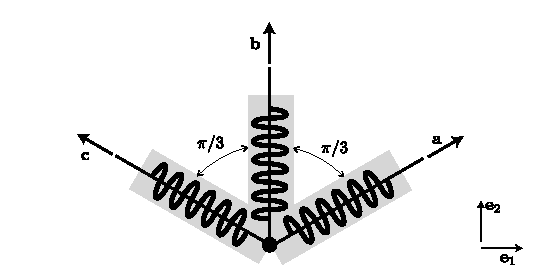
\includegraphics[scale=1.2]{figure/cinematica/rosetta.pdf}
	\end{center}
	
	\begin{svolgimento}
		Let us denote by
		\begin{equation}
			\ab = \frac{\sqrt{3}}{2}\eb_{1} + \frac12 \eb_2, \qquad \bb=\eb_2, \qquad \cb = -\frac{\sqrt{3}}{2}\eb_{1} + \frac12 \eb_2
		\end{equation}
		the unit vectors defining the three directions of the rosette. We need to solve the system
		\begin{equation}
			\begin{cases}
				\Eb \ab \cdot \ab = \dfrac{1}{2}(3 E_{11} + 2\sqrt{3} E_{12} + E_{22}) = \varepsilon_a,\\[.2cm]
				\Eb \bb \cdot \bb = E_{22} = \varepsilon_b,\\[.2cm]
				\Eb \cb \cdot \cb = \dfrac14 (3E_{11} - 2\sqrt{3}E_{12} + E_{22}) = \varepsilon_c,
			\end{cases}
		\end{equation}
		for the unknowns $E_{11}$, $E_{12}$, and $E_{22}$. The solution is
		\begin{equation}
			E_{11} = \frac13(2\varepsilon_a - \varepsilon_b + 2\varepsilon_c), \qquad E_{12} = \frac{\varepsilon_a - \varepsilon_c}{\sqrt{3}}, \qquad 
			E_{22} = \varepsilon_b.
		\end{equation}
	\end{svolgimento}
	
\end{exercise}

\begin{exercise}\label{defmedia}
	Let $\bar\Eb$ be the average strain of a configuration ${\Omega}$:
	\begin{equation}
		\bar{\Eb} = \frac{1}{\textrm{vol}({\Omega})}\int_{\Omega}\Eb.
	\end{equation}
	Prove that the average strain depends only on the displacement $\ub$ on the boundary and, in particular,
	\begin{equation}
		\bar{\Eb} = \frac{1}{2\textrm{vol}(\Omega)}\int_{\partial{\Omega}} \ub \otimes \nb + \nb \otimes \ub
	\end{equation}
	where $\textrm{vol}(\Omega)$ is the volume of $\Omega$ and $\nb$ is the normal to the boundary of ${\Omega}$.
	
	\begin{svolgimento}
		We use the following version of the divergence theorem (see \eqref{theodiv}):
		\begin{equation}
			\int_{\Omega} \nabla \varphi = \int_{\partial\Omega} \varphi \nb,
		\end{equation}
		where $\varphi$ is a scalar field. Choose $\varphi = \ub \cdot \ab$, with $\ab \in \Vc$ constant. We have
		\begin{equation}
			(\nabla \varphi)_i = \varphi,_i \eb_i = (\ub,_{i}\cdot \ab) \eb_i = (\eb_i \otimes \ub,_i) \ab = \nabla \ub^\top \, \ab.
		\end{equation}
		Therefore,
		\begin{equation}
			\left( \int_{\Omega} \nabla \ub^\top \right) \ab = \int_{\partial{\Omega}} (\ub \cdot \ab) \nb = \int_{\partial{\Omega}} (\nb \otimes \ub) \ab,
		\end{equation}
		from which we conclude that
		\begin{equation}
			\int_{\Omega} \nabla \ub^\top = \int_{\partial{\Omega}} \nb \otimes \ub.
		\end{equation}
		Given the definition of $\Eb$, it is then immediate to conclude that
		\begin{equation}
			\bar{\Eb} = \frac{1}{2 \operatorname{vol}(\Omega)} \int_{\partial{\Omega}} \ub \otimes \nb + \nb \otimes \ub.
		\end{equation}
	\end{svolgimento}
\end{exercise}

\begin{exercise}
	\item Consider a disk of radius $R$ centered at the origin of the Cartesian coordinate system $\{O; x_1, x_2\}$. On the boundary of the disk, the displacement is imposed as
	\begin{equation}
		\ub(\xb) = (\alpha \eb_1 \otimes \eb_1 + \beta \eb_2 \otimes \eb_1) \xb \qquad \alpha, \beta \in \Ro.
	\end{equation}
	Determine the average strain of the disk.
	\begin{svolgimento}
		Given the geometry, it is convenient to use polar coordinates, so that the position of a generic point on the disk is
		\begin{equation}
			\xb = \rho \cos\vartheta \eb_1 + \rho \sin\vartheta \eb_2, \qquad 0 \leq \rho < R, \quad 0 \leq \vartheta < 2\pi.
		\end{equation}
		The unit normal vector to the disk is 
		\begin{equation}
			\nb = \cos\vartheta \eb_1 + \sin\vartheta \eb_2.
		\end{equation}
		With the aim of using the result from exercise \ref{defmedia}, we determine
		\begin{equation}
			\begin{aligned}
				\frac12 (\ub \otimes \nb + \nb \otimes \ub) &= \alpha R \cos^2 \vartheta \eb_1 \otimes \eb_1 + \frac{1}{2} R \cos\vartheta (\alpha \sin\vartheta + \beta \cos\vartheta) (\eb_1 \otimes \eb_2 + \eb_2 \otimes \eb_1)\\
				&+ R \beta \sin\vartheta \cos\vartheta\, \eb_2 \otimes \eb_2,
			\end{aligned}
		\end{equation}
		from which we get
		\begin{equation}
			\bar{\Eb} = \frac{1}{\pi R^2} \int_0^{2\pi} \frac12 (\ub \otimes \nb + \nb \otimes \ub) R \, d\vartheta = \alpha \eb_1 \otimes \eb_1 + \frac \beta 2 (\eb_1 \otimes \eb_2 + \eb_2 \otimes \eb_1).
		\end{equation}
	\end{svolgimento}
\end{exercise}

\begin{exercise}
	Let  $\ub: \Omega \to \Vc$ be a displacement field tangential to the boundary of $\Omega$. Show that in infinitesimal theory, the specific volume change is, on average, zero.
	\begin{svolgimento}
		Using the result from exercise \ref{defmedia}, we can determine the average specific volume change:
		\begin{equation}
			\operatorname{tr} \bar{\Eb} = \frac{1}{\operatorname{vol}(\Omega)} \int_{\partial{\Omega}} \ub \cdot \nb = 0
		\end{equation}
		since $\ub \cdot \nb = 0$ on $\partial{\Omega}$, as $\ub$ is tangential to the boundary of $\Omega$.
	\end{svolgimento}
\end{exercise}


\section{The Compatibility Condition}

Given an arbitrary deformation field \(\Eb\), the relationship between displacement and deformation
\begin{equation}
	\Eb = \frac{1}{2} (\nabla \ub + \nabla \ub^\top)
\end{equation}
constitutes a first-order linear differential equation in the displacement field \(\ub\), whose solution is not guaranteed to exist. We will show that a \textit{necessary} condition for the existence of solutions is that the deformation field satisfies a certain compatibility condition, which is also \textit{sufficient} to guarantee existence if the domain is simply connected.

First, note that the deformation field \(\Eb\) and the infinitesimal rotation vector \(\wb\) satisfy the following condition:
\begin{equation}\label{RotE}
	\Curl \Eb = \nabla \wb.
\end{equation}
% Recall that the components of the curl of a vector \(\vb\) are 
%\begin{equation}
%(\Curl \vb)_i = \epsilon_{ijk} v_{k,j}
%\end{equation}
% where
%\begin{equation}
%\epsilon_{ijk} = \eb_i \times \eb_j \cdot \eb_k
%\end{equation}
% is the Ricci symbol (see \eqref{Ricci}).
%, such that
%\begin{equation}
%\epsilon_{ijk} = \begin{cases} +1 & \text{if all indices \(i, j, k\) are different and their sequence} \\ & \text{is an even permutation of \(1, 2, 3\)}; \\ 0 & \text{if at least two of the indices \(i, j, k\) are equal;} \\ -1 & \text{if all indices \(i, j, k\) are different and their sequence} \\ & \text{is an odd permutation of \(1, 2, 3\)}. \end{cases}
%\end{equation}
% Given a tensor field \(\Ab\), its curl is defined as:
%\begin{equation}
%(\Curl \Ab) \ab \coloneqq \Curl(\Ab^\top \ab), \qquad \forall \ab \in \Vc;
%\end{equation}
% in components:
%\begin{equation}
%	(\Curl \Ab)_{ij} = \epsilon_{ipq} A_{jq},_{p}.
%\end{equation}
To prove \eqref{RotE}, we calculate the curl of the gradient of the displacement (see \eqref{RotT}):
\begin{equation}
	(\Curl(\nabla \ub))_{ij} = \epsilon_{ipq} (\nabla \ub)_{jq,p} = \epsilon_{ipq} (u_{j,q})_p = \epsilon_{ipq} u_{j,qp} = 0;
\end{equation}
furthermore, we have
\begin{equation}
	(\Curl(\nabla \ub^\top))_{ij} = \epsilon_{ipq} (u_{q,j}),_p = \epsilon_{ipq} u_{q,jp} = (\epsilon_{ipq} u_{q,p}),_j = 2 w_{i,j} = 2 (\nabla \wb)_{ij}.
\end{equation}
In the last equality, we introduced the vector
\begin{equation}
	\wb \coloneqq \frac{1}{2} \Curl \ub;
\end{equation}
since, using \eqref{epsdel}, we can write the following sequence of equalities:
\begin{equation}
	\begin{aligned}
		(\wb \times \ab)_i &= \epsilon_{ijk} w_j a_k = \frac{1}{2} \epsilon_{ijk} \epsilon_{jpq} u_{q,p} a_k \\
		&= -\frac{1}{2} \epsilon_{jik} \epsilon_{jpq} u_{q,p} a_k = -\frac{1}{2} (\delta_{ip} \delta_{kq} - \delta_{iq} \delta_{kp}) u_{q,p} a_k \\
		&= \frac{1}{2} (u_{i,k} - u_{k,i}) a_k = \frac{1}{2} (\nabla \ub - \nabla \ub^\top)_{ik} a_k = W_{ik} a_k = (\Wb \ab)_i,
	\end{aligned}
\end{equation}
for every \(\ab\), we can identify \(\wb\) with the axial part of the infinitesimal rotation tensor \(\Wb\), so that
\begin{equation}
	\Wb \ab = \frac{1}{2} \Curl \ub \times \ab.
\end{equation}

We then conclude that
\begin{equation}
	\Curl \Eb = \frac{1}{2} \big( \Curl (\nabla \ub) + \Curl (\nabla \ub^\top) \big) = \nabla \wb.
\end{equation}
Applying the curl operator again to \eqref{RotE}, we conclude that a necessary condition for the existence of a displacement field is that \(\Eb\) satisfies the following \textit{compatibility condition}:
\begin{definition}
	\begin{equation}\label{RotRot}
		\Curl \Curl \Eb = \mathbf{0}.
	\end{equation}
\end{definition}

We now prove that the condition \eqref{RotRot} is not only sufficient but also necessary, if the domain is simply connected; in other words, if \(\Curl \Curl \Eb = \mathbf{0}\), then there certainly exists a vector field \(\ub\) such that \(\Eb = \sym \nabla \ub\).

To prove this, we need two preparatory results:
\begin{enumerate}
	\item Let \(\Tb \in \Lin\) such that \(\Curl \Tb = \mathbf{0}\), then there exists a vector field \(\ub\) such that\footnote{To prove this, consider the vectors
		\begin{equation}
			\ab_i = \Tb^\top \eb_i,
		\end{equation}
		where \(\eb_i\) are the basis vectors; we have that
		\begin{equation}
			\Curl \ab_i = \Curl (\Tb^\top \eb_i) = \Curl(\Tb^\top) \eb_i = 0
		\end{equation}
		and thus there exist scalar fields \(u_i\) such that \(\ab_i = \nabla u_i\).
		%
		Define \(\ub \coloneqq u_i \eb_i\); then
		\begin{equation}
			\ab_i = \nabla u_i = \nabla(\ub \cdot \eb_i) = (\nabla \ub)^\top \eb_i = \Tb^\top \eb_i,
		\end{equation}
		which gives \eqref{Tnabu}.}
	\begin{equation}\label{Tnabu}
		\Tb = \nabla \ub.
	\end{equation}
	\item Let \(\Tb \in \Lin\) such that \(\Curl \Tb = \mathbf{0}\) and \(\operatorname{tr} \Tb = 0\), then there exists \(\Wb \in \Skw\) such that\footnote{
		To prove this: let \(\ub\) be the vector defined in the previous note and \(\Wb\) the skew-symmetric tensor associated with \(-\ub\). Then
		\begin{equation}
			\Div \ub = \operatorname{tr} \nabla \ub = \operatorname{tr} \Tb = 0.
		\end{equation}
		By \eqref{identitadiff}$_9$
		\begin{equation}
			-\Curl \Wb = (\Div \ub)\Ib - \nabla \ub = -\nabla \ub = -\Tb,
		\end{equation}
		which gives the result.
	}
	\begin{equation}
		\Tb = \Curl \Wb.
	\end{equation}
\end{enumerate}

Now, let's return to proving that if \(\Curl \Curl \Eb = \mathbf{0}\), then there exists a vector field \(\ub\) such that \(\Eb = \sym \nabla \ub\). Assume that \(\Curl \Curl \Eb = \mathbf{0}\) in \(\Omega\). Let \(\Ab = \Curl \Eb\); since \(\Eb \in \Sym\),
\eqref{identitadiff}$_8$ implies that
\begin{equation}
	\operatorname{tr} \Ab = 0.
\end{equation}
Since \(\Curl \Ab = \mathbf{0}\), there exists a tensor field \(\Wb \in \Skw\) such that
\begin{equation}
	\Ab = -\Curl \Wb.
\end{equation}
Since \(\Ab = \Curl \Eb\),
\begin{equation}
	\Curl (\Eb + \Wb) = \mathbf{0};
\end{equation}
therefore, there exists a vector field \(\ub\) such that
\begin{equation}
	\Eb + \Wb = \nabla \ub.
\end{equation}
Taking the symmetric part of the last equality, we conclude that there exists \(\ub\) such that
\begin{equation}
	\Eb = \sym \nabla \ub.
\end{equation}




\part{Basic Mechanical Principles}
\chapter{Mass Balance}

The body $\Bc$ is treated as a continuum, being the topological image of a domain. The mass distribution is, for now, left unspecified. In continuum mechanics, primary interest lies in mass distributions that are absolutely continuous with respect to volume.

Let $\Pi\subset\Omega$ a part of $\Omega$; here and henceforth we denote by $\Pi_t=\fb_t(\Pi)$ the image of $\Pi$ under the motion $\fb_t$. We write $\rho_{\rm ref}(\xb)>0$ for the referential mass density at the  point $\xb$  in the referential region $\Omega$ identifying the body, so that
\begin{equation}
	\int_{\Pi}\rho_{\rm ref}(\xb)\,\dd v_{\rm ref}
\end{equation}
is the mass of the region $\Pi$; we have specified the integration $\dd v_{\rm ref}$ to stress that it concerns the referential configuration.

Analogously we can introduce the current mass density $\rho(\yb,t)$ at $\yb\in\Pi_t$, so that
\begin{equation}
	\int_{\Pi_t}\rho(\yb,t)\dd v_{\rm cur}
\end{equation}
represents the mass of the region $\Pi_t$ occupied at time $t$. 

Balance of mass is the requirement that
\begin{equation}
	\int_{\Pi}\rho_{\rm ref}(\yb)\,\dd v_{\rm ref}=\int_{\Pi_t}\rho(\yb,t)\dd v_{\rm cur}
\end{equation}
for every region. The right hand side only depends on time, and then
\begin{equation}\label{bm}
	\left( \int_{\Pi_t}  \rho(\yb,t)\dd v_{\rm cur}\right)^{\dotb}=0
\end{equation}

We recall that
\begin{equation}
	\dd v_{\rm cur}=(\det\Fb)\,\dd v_{\rm ref}.
\end{equation}
We now need to state how to perform the time derivative on \eqref{bm}. Let $\varphi$ a  field given in the current representation. We have that
\begin{equation}
	\begin{aligned}
		\left( \int_{\Pi_t}  \varphi\dd v_{\rm cur}\right)^{\dotb}&=\left( \int_{\Pi}(\det\Fb)\varphi  \dd v_{\rm ref} \right)^{\dotb}\\
		&=\int_{\Pi}(\det\Fb)^{\dotb}\varphi+\dot{\varphi}(\det\Fb).
	\end{aligned}
\end{equation}
To go further we need some algebra. In particular, we need the following relation:
\begin{equation}\label{devdet}
	\partial_{\Ab}(\det\Ab)=\Ab^*
\end{equation}
and  the fact that $\operatorname{tr}{(\Ab\Bb)}=\Ab\cdot\Bb^\top$. With this, we find 
\begin{equation}
	(\det\Fb)^{\dotb}=\partial_{\Fb}(\det\Fb)\cdot\dot{\Fb}=\Fb^*\cdot\dot{\Fb}=(\det\Fb)\Fb^{-\top}\cdot\dot{\Fb}=(\det\Fb)\operatorname{tr}(\dot{\Fb}\Fb^{-1})=(\det\Fb)\operatorname{tr}\Lb=(\det\Fb)\dive\vb,
\end{equation}
whence 
\begin{equation}
	(\det\Fb)^{\dotb}=(\det\Fb)\dive \vb
\end{equation}
holds true. We therefore  conclude that
\begin{equation}
	\begin{aligned}
		\left( \int_{\Pi_t}  \varphi\dd v_{\rm cur}\right)^{\dotb}&=\int_{\Pi}(\dot{\varphi}+\varphi\dive\vb)(\det\Fb)\,\dd v_{\rm ref},
	\end{aligned}
\end{equation}
whence we get the 
\begin{definition}
\textit{\textbf{Reynolds' transport theorem}}
\begin{equation}\label{reyn}
	\begin{aligned}
		\left( \int_{\Pi_t}  \varphi\dd v_{\rm cur}\right)^{\dotb}=\int_{\Pi_t}(\dot{\varphi}+\varphi\dive\vb)\dd v_{\rm cur}.
	\end{aligned}
\end{equation}
\end{definition}
With this, \eqref{bm} reads
\begin{equation}
	\int_{\Pi_t}(\dot{\rho}+\rho\dive\vb)\dd v_{\rm cur}=0
\end{equation}
$\forall\,\Pi_t$; this quantification allows to determine the:
\begin{definition}
 \textit{\textbf{Local mass balance}}
\begin{equation}\label{masbal}
	\dot{\rho}+\rho\dive\vb=0.
\end{equation}
\end{definition}

The first term represents the rate of increase of mass, which  must be compensated by the net mass flux out of the volume (second term). To understand this, consider a small fixed control volume in space; the idea is that mass can enter or leave this volume due to the motion of the material --- that is, due to the velocity field $\vb$.

Now $\dive\vb$ measures how much the velocity field is ``spreading out'' or ``converging'' at a point, so it is the rate of volumetric expansion; if $\dive\vb>0$, then the volume at that point is expanding, so material is moving away from the point --- suggesting mass is leaving the control volume;  if $\dive\vb<0$, the volume is shrinking --- mass is entering. The quantity  $\rho \dive \vb$  gives the net rate at which mass flows out of an infinitesimal volume due to the expansion or contraction of the material.

\begin{remark}
In order to prove \eqref{devdet}, for $f(\Ab)$ a scalar-valued function of a second order $\Ab$, let us define its directional derivative in direction $\Hb\in\Lin$ as
\begin{equation}
\partial_\Ab f(\Ab)\cdot \Hb=\left.\frac{\dd}{\dd \varepsilon}f(\Ab+\varepsilon\Hb)\right|_{\varepsilon=0}.
\end{equation}
Let $f(\Ab)=\det\Ab$. Assume that $\Ab$ is invertible; then
\begin{equation}
	\Ab+\varepsilon\Hb=\Ab(\Ib+\varepsilon\Ab^{-1}\Hb),
\end{equation}
which is easily proved:
\begin{equation}
\Ab(\Ib+\varepsilon\Ab^{-1}\Hb)=\Ab+\varepsilon\Ab\Ab^{-1}\Hb=\Ab+\varepsilon\Hb.
\end{equation}
Therefore
\begin{equation}
	\det(\Ab+\varepsilon\Hb)=\det \Big(\Ab(\Ib+\varepsilon\Ab^{-1}\Hb)  \Big)=\det\Ab \, \det(\Ib+\varepsilon\Ab^{-1}\Hb),
\end{equation}
where we have made use of the Binet theorem, stating that $\det(\Ab\Bb)=\det\Ab\,\det\Bb$, for all $\Ab,\Bb\in\Lin$.

To determine $\det(\Ib+\varepsilon\Ab^{-1}\Hb)$ for $\varepsilon$ small, we notice that, for $\Bb \in\Lin$ the eigenvalues of $\Ib+\varepsilon\Bb$ are $1+\varepsilon\lambda_i$, being $\lambda_i$ the eigenvalues of $\Bb$ (this is due to the fact that $\Bb$ and $\Ib+\varepsilon\Bb$ are simultaneously triangularizable.). Therefore
\begin{equation}
	\det(\Ib+\varepsilon\Bb)=\prod_{i_1}^3(1+\varepsilon\lambda_i)=1+\varepsilon\sum_{i=1}^3\lambda_i+o(\varepsilon)=1+\varepsilon\operatorname{tr}\Bb+o(\varepsilon).
\end{equation}
Therefore, for $\varepsilon$ small, we can write
\begin{equation}
\det(\Ib+\varepsilon\Ab^{-1}\Hb)=1+\varepsilon\operatorname{tr}(\Ab^{-1}\Hb)=1+\varepsilon\Ab^{-\top}\cdot\Hb,
\end{equation}
and then
\begin{equation}
		\det(\Ab+\varepsilon\Hb)=\det(\Ab)+\varepsilon(\det\Ab)\Ab^{-\top}\cdot\Hb.
		\end{equation}

Therefore
\begin{equation}
(\partial_\Ab \det\Ab)\cdot \Hb=\left.\frac{\dd}{\dd \varepsilon}\det(\Ab+\varepsilon\Hb)\right|_{\varepsilon=0}=(\det\Ab)\Ab^{-\top}\cdot\Hb,
\end{equation}
which allows to conclude that 
\begin{equation}
	\partial_\Ab \det\Ab=(\det\Ab)\Ab^{-\top}.
\end{equation}

\end{remark}


\chapter{Force and Moment Balance}


Once a configuration $\Omega$ and a deformation $\fb(\Omega)$ are given, we address the problem of modeling the mechanical interactions that accompany them, both between parts of $\Omega$ and between $\Omega$ and the surrounding environment.

\section{Force Systems}

The simplest types of mechanical interactions are described by \textit{forces}. Over time, various concepts of \textit{force systems} have been developed with the goal of abstracting from experience and thus reflecting in a model a set of salient features of the actions on the body and the environment under consideration, both separately and when they come into contact.

The world around us offers examples of \textit{surface} actions on a body, such as the action of the wind on a sail, and \textit{volume} actions at a distance, such as gravity. The creation of a concept of a force system that efficiently accounts for these surface-contact and volume-distance interactions, as well as the creation of the corresponding notion of stress, is essentially due to \textsc{Leonhard Euler} (1707--1783) and \textsc{Augustin-Louis Cauchy} (1789--1857).

%\section{Force Systems}
Given a configuration $\widetilde{\Omega}=\fb(\Omega)$, a (Cauchy) force system formally consists of two fields:
\begin{itemize}
	\item the \textit{distance forces} $\bb(\yb)$ acting in $\widetilde\Omega$;
	\item the \textit{contact forces} $\sb(\yb)$, acting on the boundary of $\widetilde\Omega$.
\end{itemize}
The distance forces have the physical dimensions of force per unit volume, which is why they are sometimes called volume forces; the contact forces have the physical dimensions of force per unit surface area.

Given a configuration $\widetilde{\Omega}$, we define the \textit{resultant} of the forces acting in $\widetilde{\Omega}$ as
\begin{definition}
	\begin{equation}
		\rb(\widetilde{\Omega}) = \int_{\widetilde{\Omega}} \bb(\yb) + \int_{\partial\widetilde{\Omega}} \sb(\yb).
	\end{equation}
\end{definition}
We also introduce the \textit{resultant moment} with respect to the point $\yb_0$ as
\begin{definition}
	\begin{equation}
		\mb_{\yb_0}(\widetilde{\Omega}) = \int_{\widetilde{\Omega}} (\yb - \yb_0) \times \bb(\yb) + \int_{\partial\widetilde{\Omega}} (\yb - \yb_0) \times \sb(\yb).
	\end{equation}
\end{definition}


\section{Internal Actions: Stress}

The characterization of internal actions qualifies the type of continuous model being introduced; we will limit our discussion to Cauchy's model.

Crucial in the description of continuous bodies \textit{à la} Cauchy is the concept of internal action (or contact interaction). The idea, dating back to Euler, is to consider a part of the set $\widetilde{\Omega}$ and recognize that it exchanges interactions with the complementary part, which need to be characterized. This characterization specifically qualifies the class of continuous bodies we consider. In this discussion, we will only address the so-called \textit{Cauchy continua}, although this does not exhaust the class of models available for characterizing contact interactions.

Given a configuration $\widetilde{\Omega}$, we imagine separating the region in question into two parts through an orientable surface $\Sigma$, with normal $\nb$; we denote by $\widetilde{\Omega}^-$ the part that has the outward normal $\nb$ in $\widetilde{\Omega} \cap \Sigma$ and by $\widetilde{\Omega}^+=\widetilde{\Omega}\setminus\widetilde{\Omega}^-$. We fix a point $\yb$ in $\widetilde{\Omega} \cap \Sigma$. The part $\widetilde{\Omega}^-$ exchanges internal actions with $\widetilde{\Omega}^+$ through $\yb$, in the form of contact interactions, which need to be characterized.

To do this, consider a ball $B(\yb, \varepsilon)$ of radius $\varepsilon$ for $\yb$, and evaluate the resultant and the resultant moment of the forces that the region $\widetilde{\Omega}^+$ exerts on $\widetilde{\Omega}^-$ through the surface $\Sigma \cap  B(\yb,\varepsilon)$:
\begin{equation}
	\rb\big(\yb, \Sigma\cap B(\yb,\varepsilon)\big), \qquad \mb_\yb\big(\yb, \Sigma\cap B(\yb,\varepsilon)\big).
\end{equation}

\begin{figure}
	\centering
	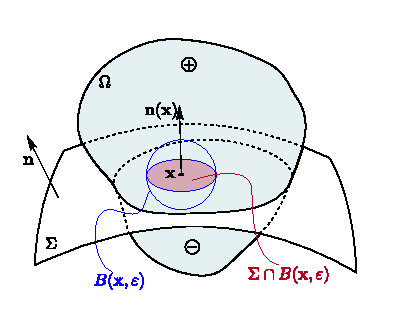
\includegraphics[scale=1.2]{figure/equilibrio/eulero3d}
	\caption{}
	\label{fig:eulero3d}
\end{figure}

Assume, according to the so-called \textit{Cauchy postulate}, that for every $\yb \in \Sigma$ there exists a $\tb(\yb; \Sigma)$ such that
\begin{definition}
	\begin{equation}
		\lim_{\varepsilon\to 0}\frac{\rb\big(\yb, \Sigma\cap B(\yb,\varepsilon)\big)}{A\big( \Sigma\cap B(\yb,\varepsilon)}=\tb(\yb, \Sigma)
	\end{equation}
\end{definition}
and
\begin{definition}
	\begin{equation}
		\lim_{\varepsilon\to 0}\frac{\mb_\yb\big(\yb, \Sigma\cap B(\yb,\varepsilon)\big)}{A\big(\yb, \Sigma\cap B(\yb,\varepsilon)}=\mathbf{0},
	\end{equation}
\end{definition}
where $A\big(\Sigma\cap B(\yb,\varepsilon)$ is the area of the surface $\Sigma\cap B(\yb,\varepsilon)$.

The field $\tb(\yb;\Sigma)$ is called the \textit{stress} and is thus the surface density of the resultant actions that the region $\widetilde{\Omega}^+$ exerts on the region $\widetilde{\Omega}^-$ through the surface $\Sigma$ at $\yb$. The density of the resultant moment is instead assumed to be zero. This choice characterizes \textit{Cauchy continua}. There exist models in which the contact interaction is not reduced to stress, but is more complex, as the density of the resultant moment is assumed to be non-zero as well; these models are commonly referred to as \textit{polar continua}.

It is important to observe that stress depends not only on the point but also on the cutting surface. We will demonstrate that:
\begin{itemize}
	\item $\tb$ depends only on the normal $\nb$ to $\Sigma$ at $\yb$ and not on all the geometric characteristics of the cutting surface (\textit{Hamel-Noll Theorem}\footnote{This theorem, in most textbooks, is considered a postulate, often called the \textit{Cauchy postulate}. From a historical point of view, it is correct, as Cauchy did not prove it, but assumed it as a given. However, the result is a simple consequence of Euler's axioms, as shown partially by Hamel and Noll.});
	\item $\tb$ depends linearly on the normal $\nb$ (\textit{Cauchy Theorem}).
\end{itemize}


\subsection{Euler's Axiom}
Let us consider a region $\Pi \subset \widetilde{\Omega}$, whose boundary $\partial\Pi$ is composed of an external part
\begin{equation}
	\partial\Pi_e \coloneqq \partial\Pi \cap \partial \widetilde{\Omega}
\end{equation}
and an internal part
\begin{equation}
	\partial\Pi_i \coloneqq \partial\Pi \setminus \partial\Pi_e.
\end{equation}

\begin{center}
	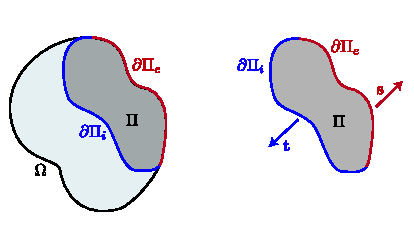
\includegraphics[scale=1.2]{figure/equilibrio/parti}
\end{center}

As stated, the resultant of the forces acting on $\bar\Pi$ is
\begin{equation}
	\rb(\Pi) = \int_{\Pi} \bb + \int_{\partial \Pi_e} \sb + \int_{\partial\Pi_i} \tb(\cdot; \partial\Pi_i),
\end{equation}
while the resultant moment with respect to the pole $\yb_0$ is
\begin{equation}
	\mb_{\yb_0}(\Pi) = \int_{\Pi} (\yb - \yb_0) \times \bb + \int_{\partial \Pi_e} (\yb - \yb_0) \times \sb + \int_{\partial \Pi_i} (\yb - \yb_0) \times \tb(\cdot; \partial\Pi_i).
\end{equation}
We assume the validity of the so-called 
\begin{definition}
	\textit{\textbf{Euler's Axiom}}. The configuration $\widetilde{\Omega}$, under the action of the volume forces $\bb$, surface forces $\sb$, and stresses $\tb$, is a configuration of equilibrium if
	\begin{equation}\label{EulAx}
		\rb(\Pi) = \mathbf{0}, \qquad \mb_{\yb_0}(\Pi) = \mathbf{0}
	\end{equation}
	for every $\Pi \subset \widetilde{\Omega}$ and for every $\yb_0$. 
\end{definition}




The body forces splits into two parts:
\begin{itemize}
	\item \textit{inertial}
	\begin{equation}
		\bb^{\rm (in)}=-\rho\dot{\vb};
	\end{equation}
	\item \textit{non-inertial}
	\begin{equation}
		\bb^{\rm (ni)}=\bb-\bb^{\rm (in)},
	\end{equation}
\end{itemize}
where the former is to be intended as a constitutive prescription. The Euler axioms then yield the \textit{balance of linear and angular momentum}:
\begin{equation}
	\rb^{\rm (ni)}(\Pi)=\dot{\lb}(\Pi), \qquad \mb_o^{\rm (ni)}(\Pi)=\dot\ab(\Pi), \quad \forall\,\Pi,
\end{equation}
where 
\begin{equation}
	\lb(\Pi):=\int_{\Pi}\rho\vb
\end{equation}
is the \textit{linear momentum} and 
\begin{equation}
	\ab(\Pi):=\int_{\Pi}\yb\times\rho\vb
\end{equation}
is the \textit{angular momentum}, and
\begin{equation}
	\rb^{\rm (ni)}(\Pi):=\int_{\partial\Pi}\tb(\nb)+\int_{\Pi}\bb^{\rm (ni)}, \qquad \mb_o^{\rm (ni)}(\Pi):=\int_{\partial\Pi}\yb\times\tb(\nb)+\int_{\Pi}\yb\times\bb^{\rm (ni)}.
\end{equation}

\begin{remark}
Given any rigid velocity field 
\begin{equation}
	\wb(\yb,t)=\wb_o(t)+\omegab(t)\times\yb
\end{equation}
and any current region $\Pi$, we define the \textit{power expended on $\Pi$ over the rigid velocity field} $\wb$
\begin{equation}
	\Wc_{\rm rig}(\Pc,\wb):=\int_{\partial\Pc}\tb(\nb)\cdot\wb+\int_{\Pi}\bb\cdot\wb.
\end{equation}
This notion has an interesting and important consequence. Since
\begin{equation}
	\begin{aligned}
		\Wc_{\rm rig}(\Pc,\wb)&=\left(\int_{\partial\Pi}\tb(\nb) + \int_{\Pi}\bb \right)\cdot \wb_o+\int_{\partial\Pi}\tb(\nb)\cdot\omegab_o\times\yb+\int_{\Pi}\bb\cdot \omegab_o\times\yb\\
		&=\rb(\Pi)\cdot\wb_o+\mb_o(\Pi)\cdot\omegab_o,
	\end{aligned}
\end{equation}
we can conclude that \textit{a system of forces is balanced if and only if the power  expended on each part $\Pi$ over a rigid velocity field vanishes}.
\end{remark}

Starting from Euler's axiom, which expresses a condition of global equilibrium, we will derive pointwise conditions. In particular, we will use the following 

\begin{definition}
	\textit{\textbf{Localization Lemma}}. If $B(\yb_0, \varepsilon) \coloneqq \{\yb : |\yb - \yb_0| \leq \varepsilon \}$ is the ball of radius $\varepsilon$ centered at $\yb_0$ with volume $V\big(B(\yb_0, \varepsilon)\big)$, $\yb_0 \in \Vc$, and $\gb$ is a continuous function in a neighborhood of $\yb_0$, then
\begin{equation}\label{lemma3}
	\lim_{\varepsilon \to 0}\frac{1}{V\big(B(\yb_0, \varepsilon)\big)}\int_{B(\yb_0, \varepsilon)} \gb (\yb) \, \dd \yb = \gb(\yb_0).
\end{equation}
\end{definition}

We will use this lemma to prove the Hamel-Noll theorem and the Cauchy theorem.

%\begin{remark}
%	We prove the localization lemma. 
%	Starting from the given expression:
%	\[
%	\frac{1}{V(B(\yb_0, \varepsilon))} \int_{B(\yb_0, \varepsilon)} \gb(\yb) \, \dd \yb.
%	\]
%	Since \( \gb \) is continuous at \( \yb_0 \), we can express \( \gb(\yb) \) as:
%	\[
%	\gb(\yb) = \gb(\yb_0) + (\gb(\yb) - \gb(\yb_0)).
%	\]
%	Substituting this expression into the integral, we get:
%	\[
%	\begin{aligned}
%		\frac{1}{V(B(\yb_0, \varepsilon))} \int_{B(\yb_0, \varepsilon)} \gb(\yb) \, \dd \yb = &\frac{1}{V(B(\yb_0, \varepsilon))} \int_{B(\yb_0, \varepsilon)} \gb(\yb_0) \, \dd \yb \\
%		&+ \frac{1}{V(B(\yb_0, \varepsilon))} \int_{B(\yb_0, \varepsilon)} (\gb(\yb) - \gb(\yb_0)) \, \dd \yb.
%	\end{aligned}
%	\]
%	The first term is easy to compute:
%	\[
%	\frac{1}{V(B(\yb_0, \varepsilon))} \int_{B(\yb_0, \varepsilon)} \gb(\yb_0) \, \dd \yb = \frac{1}{V(B(\yb_0, \varepsilon))} \cdot V(B(\yb_0, \varepsilon)) \cdot \gb(\yb_0) = \gb(\yb_0).
%	\]
%	Now consider the second term:
%	\[
%	\frac{1}{V(B(\yb_0, \varepsilon))} \int_{B(\yb_0, \varepsilon)} (\gb(\yb) - \gb(\yb_0)) \, \dd \yb.
%	\]
%	Since \( \gb \) is continuous at \( \yb_0 \), for every \( \delta > 0 \), there exists an \( \varepsilon > 0 \) sufficiently small such that:
%	\[
%	|\gb(\yb) - \gb(\yb_0)| < \delta \quad \text{for every} \quad \yb \in B(\yb_0, \varepsilon).
%	\]
%	This allows us to estimate the second term:
%	\[
%	\left| \frac{1}{V(B(\yb_0, \varepsilon))} \int_{B(\yb_0, \varepsilon)} (\gb(\yb) - \gb(\yb_0)) \, \dd \yb \right| \leq \frac{1}{V(B(\yb_0, \varepsilon))} \int_{B(\yb_0, \varepsilon)} |\gb(\yb) - \gb(\yb_0)| \, \dd \yb.
%	\]
%	Since \( |\gb(\yb) - \gb(\yb_0)| < \delta \) for every \( \yb \in B(\yb_0, \varepsilon) \), we get:
%	\[
%	\frac{1}{V(B(\yb_0, \varepsilon))} \int_{B(\yb_0, \varepsilon)} |\gb(\yb) - \gb(\yb_0)| \, \dd \yb \leq \delta.
%	\]
%	
%	Since \( \delta \) can be made arbitrarily small by choosing \( \varepsilon \) sufficiently small, we conclude that:
%	\[
%	\lim_{\varepsilon \to 0} \frac{1}{V(B(\yb_0, \varepsilon))} \int_{B(\yb_0, \varepsilon)} (\gb(\yb) - \gb(\yb_0)) \, \dd \yb = 0.
%	\]
%	
%	Combining the results, we get:
%	\[
%	\lim_{\varepsilon \to 0} \frac{1}{V(B(\yb_0, \varepsilon))} \int_{B(\yb_0, \varepsilon)} \gb(\yb) \, \dd \yb = \gb(\yb_0).
%	\]
%	
%	Therefore, the theorem is proved.
%\end{remark}


\subsection{The Hamel-Noll Theorem}
We state the 
\begin{definition}
	\textbf{\textit{Hamel-Noll Theorem}} Given two surfaces $\Sigma$ and $\hat\Sigma$ that have at least one common point $\yb_0 \in \Sigma \cap \hat{\Sigma} \subset \widetilde{\Omega}$ and share the same normal vector $\nb$ at $\yb_0$, then for an equilibrium configuration $\Omega$ under the action of $\{\bb, \sb, \tb\}$, we have
	\begin{equation}\label{HN0}
		\tb(\yb_0;\Sigma) = \tb(\yb_0;\hat\Sigma).
	\end{equation}
\end{definition}

In other words, the stress depends only on the normal vector; we can therefore define
\begin{equation}
	\tb(\yb_0, \nb) \coloneqq \tb(\yb_0; \Sigma) = \tb(\yb_0; \hat\Sigma).
\end{equation}

We now prove the theorem. The surface $\Sigma$ divides the region $\Omega$ into two parts, $\Omega^-$ and $\Omega^+$; similarly, the surface $\hat{\Sigma}$ divides the region $\Omega$ into two parts, $\hat\Omega^-$ and $\hat\Omega^+$. Consider the semi-cylinder $C_\varepsilon$ with an axis passing through $\yb_0$, a circular base of radius $\varepsilon$ orthogonal to $\nb$, and at a distance of $\varepsilon^2$ from $\nb$, contained in $\Omega^- \cap \hat{\Omega}^-$.

We define
\begin{equation}
	P_{\varepsilon} \coloneqq C_\varepsilon \cap \Omega^-, \qquad \hat{P}_{\varepsilon} \coloneqq C_\varepsilon \cap \hat\Omega^-
\end{equation}
as the parts of the semi-cylinder contained in $\Omega^-$ and $\hat\Omega^-$. 

\begin{center}
	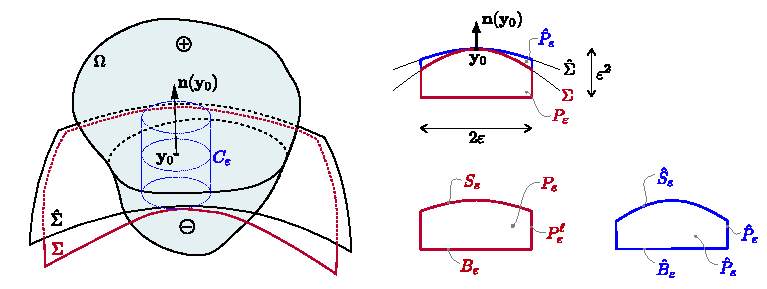
\includegraphics[scale=1.2]{figure/equilibrio/hamelnoll}
\end{center}

We write the translational equilibrium of $P_{\varepsilon}$:
\begin{equation}\label{rHN}
	\rb(P_\varepsilon) = \int_{P_\varepsilon} \bb + \int_{B_\varepsilon} \tb(\cdot; B_\varepsilon) + \int_{P^\ell_\varepsilon} \tb(\cdot; P^\ell_\varepsilon) + \int_{S_\varepsilon} \tb(\cdot; \Sigma) = \mathbf{0},
\end{equation}
where $B_\varepsilon$ is the base and $P^\ell_\varepsilon$ is the lateral surface of $P_\varepsilon$, while $S_\varepsilon \coloneqq P_\varepsilon \cap \Sigma$ is the "upper base," obtained by intersecting $P_{\varepsilon}$ with the surface $\Sigma$. We observe that the volume $V(P_\varepsilon)$ is of order $O(\varepsilon^4)$, the area $A(P_\varepsilon^\ell)$ is of order $O(\varepsilon^3)$, the area $A(B_\varepsilon)$ is of order $O(\varepsilon^2)$, and the area $A(S_\varepsilon)$ is of order $\varepsilon^2$.

We divide \eqref{rHN} by $A(S_\varepsilon)$ and rewrite it to apply the localization lemma:
\begin{equation}
	\begin{aligned}
		&\frac{V(P_\varepsilon)}{A(S_\varepsilon)} \, \frac{1}{V(P_\varepsilon)} \int_{P_\varepsilon} \bb +
		\frac{A(B_\varepsilon)}{A(S_\varepsilon)} \frac{1}{A(B_\varepsilon)} \int_{B_\varepsilon} \tb(\cdot; B_\varepsilon) + \frac{A(P^\ell_\varepsilon)}{A(S_\varepsilon)} \int_{P^\ell_\varepsilon} \tb(\cdot; P^\ell_\varepsilon) \\
		& + \frac{1}{A(S_\varepsilon)} \int_{S_\varepsilon} \tb(\cdot; \Sigma) = \mathbf{0}.
	\end{aligned}
\end{equation}
As $\varepsilon$ tends to zero,
\begin{equation}
	\frac{V(P_\varepsilon)}{A(S_\varepsilon)} \to 0, \quad \frac{A(P^\ell_\varepsilon)}{A(S_\varepsilon)} \to 0, \quad \frac{A(B_\varepsilon)}{A(S_\varepsilon)} \to 1, \quad \frac{1}{A(S_\varepsilon)} \int_{S_\varepsilon} \tb(\cdot; S_\varepsilon) \to \tb(\yb_0; \Sigma)
\end{equation}
and thus
\begin{equation}\label{HN1}
	\tb(\yb_0; \Sigma) + \lim_{\varepsilon \to 0} \frac{1}{A(B_\varepsilon)} \int_{B_\varepsilon} \tb(\cdot; B_\varepsilon) = \mathbf{0}.
\end{equation}

Now, requiring that the equilibrium condition holds for $\hat P_\varepsilon$, we get
\begin{equation}
	\rb(\hat P_\varepsilon) = \int_{\hat P_\varepsilon} \bb + \int_{B_\varepsilon} \tb(\cdot; B_\varepsilon) + \int_{\hat P^\ell_\varepsilon} \tb(\cdot; \hat P^\ell_\varepsilon) + \int_{\hat S_\varepsilon} \tb(\cdot; \hat{\Sigma}) = \mathbf{0}.
\end{equation}
Proceeding as for $P_\varepsilon$, we obtain
\begin{equation}\label{HN2}
	\tb(\yb_0; \hat\Sigma) + \lim_{\varepsilon \to 0} \frac{1}{A(B_\varepsilon)} \int_{B_\varepsilon} \tb(\cdot; B_\varepsilon) = \mathbf{0}.
\end{equation}
From \eqref{HN1} and \eqref{HN2}, we immediately obtain \eqref{HN0}.



\subsection{The Cauchy Theorem}

Let’s immediately state the theorem:

\begin{definition}
	Let \(\Omega\) be an equilibrium configuration for \(\{\bb, \sb, \tb\}\). Then the stress depends linearly on the normal; in particular, there exists a tensor field \(\Tb \,:\, \Omega \to \Lin\), called the \textit{Cauchy stress tensor}, such that
	\[
	\tb(\yb_0, \nb) = \Tb(\yb_0) \nb,
	\]
	for every \(\yb_0 \in \Omega\) and every unit vector \(\nb\).
\end{definition}

The theorem is a milestone in continuum mechanics, as Cauchy himself proudly recognized. The proof, published in 1823, elegantly uses a construction based on certain geometric properties of the tetrahedron, which we will recall shortly. One undeniable value of this proof is that it is constructive: not only does it produce an existence result for the stress tensor, but it also provides an explicit representation of it.

Next, we will first recall some geometric properties of the tetrahedron, which are essential for the proof, and then establish a preparatory result, usually referred to as the \textit{Cauchy Lemma}.

\subsubsection{Geometry of the Tetrahedron} 
Consider a tetrahedron with three mutually orthogonal faces with area \(A_i\) and external normal \(\eb_i\), while the inclined face has area \(A\) and external normal \(\nb\), with \(\nb \cdot \eb_i > 0\) for \(i = 1, 2, 3\). We want to prove the following property:
\begin{equation}\label{Ai}
	\frac{A_i}{A} = \nb \cdot \eb_i.
\end{equation}
Let \(\vb_i\) denote the three vectors that go from the origin to the intersection point \(P_i\) of the oblique plane with the axes parallel to \(\eb_i\).

\begin{center}
	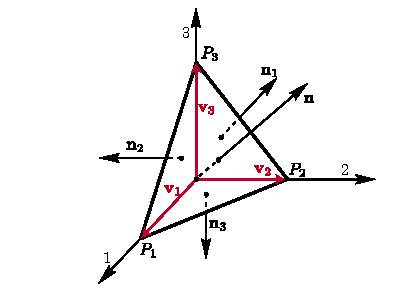
\includegraphics[scale=1.2]{figure/equilibrio/tetraedro}
\end{center}

Observe that \(\overrightarrow{P_1P_2} = \vb_2 - \vb_1\) and \(\overrightarrow{P_1P_3} = \vb_3 - \vb_1\). Then, using the properties of the vector cross product, we have
\[
\begin{aligned}
	A \nb &= \frac{1}{2} \overrightarrow{P_1P_2} \times \overrightarrow{P_1P_3} = \frac{1}{2} (\vb_1 \times \vb_3 - \vb_2 \times \vb_1 - \vb_1 \times \vb_3) \\
	&= A_1 \eb_1 + A_2 \eb_2 + A_3 \eb_3,
\end{aligned}
\]
from which equation \eqref{Ai} follows.

\subsubsection{Cauchy’s Lemma}
We state Cauchy’s lemma:

\begin{definition}
	The stress \(\tb(\yb_0, \nb)\) is an odd function of \(\nb\), i.e.
	\begin{equation}\label{lemmaC}
		\tb\big(\yb_0, \nb(\yb_0)\big) = -\tb\big(\yb_0, -\nb(\yb_0)\big).
	\end{equation}
\end{definition}

The physical interpretation is clear: at a point \(\yb_0\), the stress recorded on a plane with normal \(\nb\) is equal and opposite to the stress on the plane with normal \(-\nb\). This is nothing but the formalization of the \textit{action and reaction principle} in this context.

To prove this, we use an argument similar to the one used to prove the Hamel-Noll theorem. Suppose the region \(\Omega\) is separated into two parts by a surface \(\Sigma\) with normal \(\nb\) at \(\yb_0\). Consider a semi-cylinder \(C_\varepsilon\), with radius \(\varepsilon\), base \(B_\varepsilon\) situated at a distance \(\varepsilon^2\) from \(\yb_0\) and axis parallel to \(\nb\). We require that the part \(P_\varepsilon\) is in equilibrium:
\begin{equation}
	\rb(P_\varepsilon) = \int_{P_\varepsilon} \bb + \int_{B_\varepsilon} \tb(\cdot; -\nb) + \int_{P^\ell_\varepsilon} \tb(\cdot; \mb) + \int_{S_\varepsilon} \tb(\cdot; \nb) = \mathbf{0},
\end{equation}
where \(P^\ell_\varepsilon\) is the lateral surface of \(P_\varepsilon\), with outward normal \(\mb\), and \(S_\varepsilon = P_\varepsilon \cap \Sigma\). Dividing by the area \(A(S_\varepsilon)\) and taking the limit as \(\varepsilon\) goes to zero, using the usual localization lemma, we obtain
\begin{equation}
	\tb(\yb_0, -\nb(\yb_0)) + \tb(\yb_0, \nb(\yb_0)) = \mathbf{0},
\end{equation}
which gives the expected result.

\subsubsection{The Tetrahedron Argument}
Now, let’s proceed with the proof of the Cauchy theorem using the tetrahedron argument. Consider an internal part \(\Tc_\varepsilon\) of \(\Omega\), shaped like a tetrahedron with three edges passing through \(\yb_0\) and parallel to a fixed arbitrary Cartesian coordinate system. Let \(\varepsilon\) be the distance from \(\yb_0\) to the oblique face \(S_\varepsilon\), with normal \(\nb\), and area \(A(S_\varepsilon)\); the other faces \(S^i_\varepsilon\) have area \(A(S^i_\varepsilon)\) and outward normal \(-\eb_i\).

We impose equilibrium on the tetrahedron:
\begin{equation}
	\int_{\Tc_\varepsilon} \bb + \int_{S_\varepsilon} \tb(\cdot, \nb) + \sum_{i=1}^{3} \int_{S_\varepsilon^i} \tb(\cdot, -\eb_i) = \mathbf{0}.
\end{equation}
Dividing by \(A(S_\varepsilon)\), we get
\begin{equation}
	\frac{V(\Tc_\varepsilon)}{A(S_\varepsilon)} \frac{1}{V(\Tc_\varepsilon)} \int_{\Tc_\varepsilon} \bb + \frac{1}{A(S_\varepsilon)} \int_{S_\varepsilon} \tb(\cdot, \nb) + \sum_{i=1}^{3} \frac{A(S^i_\varepsilon)}{A(S_\varepsilon)} \frac{1}{A(S^i_\varepsilon)} \int_{S_\varepsilon^i} \tb(\cdot, -\eb_i) = \mathbf{0}.
\end{equation}
Using the result \eqref{Ai} and taking \(\varepsilon \to 0\), since \(V(\Tc_\varepsilon) = O(\varepsilon^3)\) and \(A(S_\varepsilon) = O(\varepsilon^2)\), we get
\[
\tb(\yb_0, \nb) = -\sum_{i=1}^{3} (\nb \cdot \eb_i) \tb(\yb_0, -\eb_i).
\]
Now, by applying Cauchy’s lemma \eqref{lemmaC}, we conclude that
\[
\tb(\yb_0, \nb) = \sum_{i=1}^{3} (\nb \cdot \eb_i) \tb(\yb_0, \eb_i) = \left(\sum_{i=1}^{3} \tb(\yb_0, \eb_i) \otimes \eb_i \right) \nb.
\]

We define
\begin{definition}
	\begin{equation}\label{Tb}
		\Tb(\yb_0) \coloneqq \sum_{i=1}^{3} \tb(\yb_0, \eb_i) \otimes \eb_i,
	\end{equation}
\end{definition}
so that we can write
\begin{definition}
	\begin{equation}\label{tTn}
		\tb(\yb_0, \nb) = \Tb(\yb_0) \nb,
	\end{equation}
\end{definition}
which shows that the stress vector at \(\yb_0\) relative to the orientation defined by \(\nb\) is obtained by applying the linear operator \(\Tb(\yb_0)\) to \(\nb\). The tensor field \(\Tb\) represents the so-called \textit{Cauchy stress tensor}. As anticipated, the proof is constructive: \(\Tb\) is explicitly represented by equation \eqref{Tb}, which reveals that to construct the stress tensor at a point, it is necessary to know the stress vector on three mutually orthogonal planes; once this is known, the stress on any plane can be determined using equation \eqref{tTn}.

\newpage
Once a basis \(\{\eb_i\}\) is chosen, we can determine the components of \(\Tb\):
\begin{equation}
	T_{ij} = \Tb \eb_j \cdot \eb_i = \tb(\cdot, \eb_i) \cdot \eb_i = t_i(\cdot, \eb_j).
\end{equation}
Thus, \(T_{ij}\) represents the \(i\)-th component of the stress on a plane with normal \(\eb_j\).

\begin{center}
	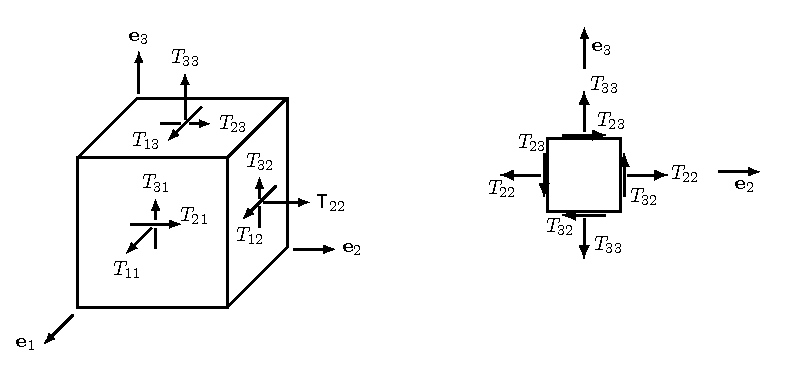
\includegraphics[scale=1]{figure/equilibrio/componenti_tensione}
\end{center}

\begin{exercise}
	At point \(\yb_0\), the stress on three planes with normal \(\eb_i\) \((i=1,2,3)\) is known:
	\begin{equation}
		\begin{aligned}
			&\tb_1(\yb_0, \eb_1) = \alpha \eb_1 - \beta \eb_3, \\
			&\tb_2(\yb_0, \eb_2) = \gamma \eb_2+\beta\eb_3, \\
			&\tb_3(\yb_0, \eb_3) = \beta (-\eb_1+\eb_2) + \gamma \eb_3.
		\end{aligned}
	\end{equation}
	Determine the stress on the plane with normal \(\nb = \frac{1}{\sqrt{2}}(\eb_1 + \eb_2)\).
	\begin{svolgimento}
		Given the stress on three planes at \(\yb_0\), the definition of \(\Tb\) allows us to determine the stress tensor:
		\begin{equation}
			\begin{aligned}
				&\Tb(\yb_0) = \alpha (\eb_1 \otimes \eb_1) + \gamma (\eb_2 \otimes \eb_2+\eb_3 \otimes \eb_3) - \beta (\eb_ 1\otimes \eb_3+ \eb_3 \otimes \eb_1-\eb_ 2\otimes \eb_3-\eb_ 3\otimes \eb_2) \\
				&\tb(\yb_0, \nb) = \Tb(\yb_0) \nb = \frac{1}{\sqrt{2}}(\alpha\eb_1+\gamma\eb_2).
			\end{aligned}
			\end{equation}
		\end{svolgimento}	
		\end{exercise}




\section{Pointwise Equilibrium Equations}
\subsection{Cauchy’s Relation for Interior Points}
Consider initially a point \(\yb_0\) inside \(\Omega\), an equilibrium configuration for \(\{\bb, \sb, \tb\}\). Let \(B(\yb_0, \varepsilon)\) be the ball centered at \(\yb_0\), with radius \(\varepsilon\), chosen small enough to ensure that \(B(\yb_0, \varepsilon) \subset \Omega\). For this ball, Euler's axiom holds:
\begin{equation}
	\int_{B(\yb_0,\varepsilon)} \bb + \int_{\partial B(\yb_0,\varepsilon)} \tb(\cdot, \nb) = \mathbf{0},
\end{equation}
or, invoking Cauchy's theorem:
\begin{equation}
	\int_{B(\yb_0, \varepsilon)} \bb + \int_{\partial B(\yb_0, \varepsilon)} \Tb \nb = \mathbf{0}.
\end{equation}
Using the divergence theorem, we obtain:
\begin{equation}\label{eq1int}
	\int_{B(\yb_0, \varepsilon)} \bb + \dive \Tb = \mathbf{0}.
\end{equation}
Dividing by \(V(B(\yb_0, \varepsilon))\) and sending \(\varepsilon\) to zero, applying the localization lemma \eqref{lemma3}, we get:
\begin{definition}
	\begin{equation}\label{bDiv}
		\bb(\yb_0) + \dive \Tb(\yb_0) = \mathbf{0},
	\end{equation}
\end{definition}
for every point \(\yb_0\) inside \(\Omega\).

%Choosing a basis \(\{\eb_i\}\), equation \eqref{bDiv} can be written componentwise:
%\begin{definition}
%	\begin{equation}
%		\begin{cases}
%			b_1 + \dfrac{\partial T_{11}}{\partial y_1} + \dfrac{\partial T_{12}}{\partial y_2} + \dfrac{\partial T_{13}}{\partial y_3} = 0,\\[.3cm]
%			b_2 + \dfrac{\partial T_{21}}{\partial y_1} + \dfrac{\partial T_{22}}{\partial y_2} + \dfrac{\partial T_{23}}{\partial y_3} = 0,\\[.3cm]
%			b_3 + \dfrac{\partial T_{31}}{\partial y_1} + \dfrac{\partial T_{32}}{\partial y_2} + \dfrac{\partial T_{33}}{\partial y_3} = 0.
%		\end{cases}
%	\end{equation}
%\end{definition}

\subsection{Cauchy’s Relation for Boundary Points}
Now, let \(\yb_0\) be a point belonging to the boundary \(\partial\Omega\). Consider the semi-cylinder \(C_\varepsilon\) with an axis passing through \(\yb_0\) and parallel to \(\nb(\yb_0)\), with a base of radius \(\varepsilon\) that is at a distance \(\varepsilon^2\) from \(\yb_0\). Let \(P_\varepsilon = \Omega \cap C_\varepsilon\). The translational equilibrium of \(P_\varepsilon\) requires that:
\begin{equation}
	\int_{P_\varepsilon} \bb + \int_{S_\varepsilon} \sb + \int_{B_\varepsilon} \Tb(-\nb) + \int_{P_\varepsilon^\ell} \Tb \mb,
\end{equation}
where \(B_\varepsilon\) is the base of \(P_\varepsilon\), \(P_\varepsilon^\ell\) is the lateral surface with outward normal \(\mb\), and \(S_\varepsilon = \partial P_\varepsilon \cap \partial \Omega\). Dividing by \(A(B_\varepsilon)\) and sending \(\varepsilon\) to zero, we obtain, using the usual argument:
\begin{equation}
	\sb(\yb_0) - \Tb(\yb_0) \nb(\yb_0) = \mathbf{0},
\end{equation}
or
\begin{definition}
	\begin{equation}\label{Tns}
		\Tb(\yb_0) \nb(\yb_0) = \sb(\yb_0)
	\end{equation}
\end{definition}
for every \(\yb_0 \in \partial \Omega\). The stress field \(\Tb(\yb_0)\) is understood as the extension to the boundary of \(\Tb\), which is actually defined on the open set \(\Omega\). Equation \eqref{Tns} establishes that, on the boundary of \(\Omega\), the stress vector is equal to the contact force exerted by the external environment on the body.

\subsection{The Symmetry of the Stress Tensor}
Up until now, we have not used the second equilibrium condition \eqref{EulAx}, which holds when a system of forces is in equilibrium. Let us now apply it to a ball \( B(\yb_0, \varepsilon) \) of radius \(\varepsilon\) centered at \(\yb_0\), using Cauchy's theorem:
\begin{equation}
	\int_{ B(\yb_0, \varepsilon)} \yb \times \bb + \int_{ \partial B(\yb_0, \varepsilon)} \yb \times \sb = \int_{ B(\yb_0, \varepsilon)} \yb \times \bb + \int_{ \partial B(\yb_0, \varepsilon)} \yb \times \Tb \nb = \mathbf{0}.
\end{equation}
Let \(\wb \in \Vc\) be a constant vector, and \(\Wb \in \Skw\) such that \(\wb \times \ab = \Wb \ab\) for any \(\ab \in \Vc\); trivially, we have
\begin{equation}
	\int_{ B(\yb_0, \varepsilon)} \wb \cdot \yb \times \bb + \int_{ \partial B(\yb_0, \varepsilon)} \wb \cdot \yb \times \Tb \nb = 0.
\end{equation}
Since \(\wb \cdot \yb \times \bb = \bb \cdot \wb \times \yb = \bb \cdot \Wb \yb\) and \(\wb \cdot \yb \times \Tb \nb = \Tb \nb \cdot \Wb \yb\), we can write:
\begin{equation}
	\int_{ B(\yb_0, \varepsilon)} \bb \cdot \Wb \yb + \int_{ \partial B(\yb_0, \varepsilon)} \nb \cdot \Tb^\top \Wb \yb = \int_{ B(\yb_0, \varepsilon)} \dive(\Tb^\top \Wb \yb) = 0,
\end{equation}
where we used the divergence theorem for the last equality. Using the identity
\begin{equation}
	\dive (\Ab \gb) = (\dive \Ab^\top) \cdot \gb + \Ab^\top \cdot \grad \gb,
\end{equation}
which is valid for any \(\Ab \in \Lin\) and \(\gb \in \Vc\), we can write
\begin{equation}
	\dive(\Tb^\top \Wb \yb) = (\dive \Tb) \cdot \Wb \yb + \Tb \cdot \Wb,
\end{equation}
and thus
\begin{equation}
	\int_{ B(\yb_0, \varepsilon)} (\bb + \dive \Tb) \cdot \Wb \yb + \Tb \cdot \Wb = 0.
\end{equation}
Note that, due to \eqref{eq1int}, the first term is zero. Dividing by the volume of the ball and taking the limit \(\varepsilon \to 0\), we then obtain
\begin{equation}
	\Tb(\yb_0) \cdot \Wb = 0.
\end{equation}
Given the arbitrariness of \(\Wb \in \Skw\), we conclude that
\begin{definition}
	\begin{equation}
		\Tb(\yb_0) \in \Sym.
	\end{equation}
\end{definition}
Thus, the stress field associated with a balanced system of forces must have \textit{symmetric} values.

\vspace{.2cm}
In conclusion, the Cauchy stress tensor associated with an equilibrium configuration for a set \(\{\bb, \sb, \tb\}\) must satisfy the following conditions:
\begin{definition}
	\begin{equation}\label{pstat}
		\begin{cases}
			\begin{array}{ll}
				\dive \Tb + \bb = \mathbf{0}, & \qquad \text{in} \; \Omega \\
				\Tb = \Tb^\top, & \qquad \text{in} \; \Omega \\
				\Tb \nb = \sb, & \qquad \text{on} \; \partial \Omega,
			\end{array}
		\end{cases}
	\end{equation}
\end{definition}

Given a configuration \(\Omega\) and a system of external forces \(\{\bb, \sb\}\), a stress field \(\Tb\) on \(\Omega\) is said to solve the corresponding \textit{static problem} if the conditions \eqref{pstat} are satisfied. The system \eqref{pstat} forms a set of 3 partial differential equations with 6 unknowns, the components of the stress tensor; in general, this problem does not admit a unique solution.


\begin{comment}
\begin{exercise}
	The stress tensor in the cube $\Omega=(-1,1)\times(-1,1)\times(-1,1)$ has a representative matrix
	\begin{equation}
		[\Tb]=\left[\begin{array}{ccc}
			\sigma y_2 y_3 & \sigma y_2^2 & \sigma(y_1-y_3) \\
			\sigma y_2^2 & \sigma y_2 & 0 \\
			\sigma(y_1-y_3) & 0 & \sigma y_3
		\end{array}\right].
	\end{equation}
	Knowing that the cube is in equilibrium, determine the applied volume and surface forces.
	\begin{svolgimento}
		Using \eqref{bDiv}, we immediately obtain
		\begin{equation}
			\begin{aligned}
				&    -b_1=(\dive \Tb)_1=T_{1j,j}=T_{11,1}+T_{12,2}+T_{13,3}=\sigma(2y_2-1), \\
				&-b_2=(\dive \Tb)_2=T_{2j,j}=T_{21,1}+T_{22,2}+T_{23,3}=\sigma, \\
				&-b_3=(\dive \Tb)_3=T_{3j,j}=T_{31,1}+T_{32,2}+T_{33,3}=2\sigma
			\end{aligned}
		\end{equation}
		or
		\begin{equation}
			\bb = \sigma\Big(  (1-2y_2)\eb_1+\eb_2+2\eb_3 \Big).
		\end{equation}
		To determine the applied surface forces on the face with normal $\eb$, we need to evaluate $\Tb$ on the plane $y_1=1$ and then observe its action on $\nb =\eb_1$:
		\begin{equation}
			[\Tb(1,y_2,y_3)]=\left[\begin{array}{ccc}
				\sigma y_2 y_3 & \sigma y_2^2 & \sigma(1-y_3) \\
				\sigma y_2^2 & \sigma y_2 & 0 \\
				\sigma(1-y_3) & 0 & \sigma y_3
			\end{array}\right]
			\left[\begin{array}{c}
				1 \\
				0 \\
				0
			\end{array}\right] = \sigma
			\left[\begin{array}{c}
				y_2 y_3 \\
				y_2^2 \\
				1 - y_3
			\end{array}\right],
		\end{equation}
		and so on for the other faces.
	\end{svolgimento}
\end{exercise}


\begin{exercise}
	Let a Cartesian coordinate system $(y_1, y_2, y_3)$ be given, and consider the cylindrical coordinate system $(\rho, \theta, z)$, with $y_1=\rho \cos \theta$, $y_2=\rho \sin \theta$, $y_3=z$, and the associated orthonormal basis $\{\eb_\rho, \eb_\theta, \eb_z\}$,
	\begin{equation}
		\eb_\rho=\cos\theta\eb_1+\sin\theta\eb_2, \quad \eb_\theta=-\sin\theta\eb_1+\cos\theta\eb_2, \quad \eb_z=\eb_3.
	\end{equation}
	The hollow cylinder
	\begin{equation}
		(R-\delta)<\rho< R, \quad 0\leq\theta<2\pi, \quad -L/2< z< L/2
	\end{equation}
	\begin{center}
		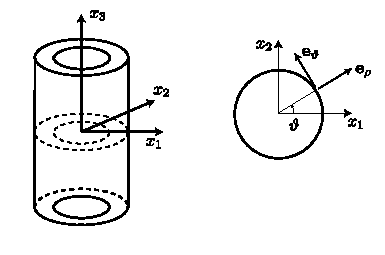
\includegraphics[scale=1.2]{figure/equilibrio/esempio13d}
	\end{center}
	is subjected to the stress
	\begin{equation}
		\Tb=2\sigma \eb_\vartheta\otimes \eb_\vartheta+\sigma \eb_z \otimes \eb_z +\frac{\tau}{R}\rho (\eb_\vartheta\otimes\eb_z+\eb_z\otimes\eb_\vartheta).
	\end{equation}
	\begin{enumerate}
		\item Write the Cartesian components of the stress field $\tb$ on the transverse section with outward normal $\eb_3$ for the origin.
		\item On the longitudinal section of the cylinder with outward normal $\eb_1$ for the origin, calculate the Cartesian components of the resultant vector $\rb$ of the stresses and the resultant moment vector $\mb_0$ with respect to the origin.
	\end{enumerate}
	\begin{svolgimento}
		\begin{enumerate}
			\item The stress on the face with normal $\eb_3$ is found using Cauchy's theorem
			\begin{equation}
				\Tb \eb_z=\sigma \eb_z +\frac{\tau}{R}\rho \eb_\vartheta=\frac{\tau}{R}(-y_2\eb_1+y_1\eb_2)+\sigma \eb_3.
			\end{equation}
			\item 
			It is necessary to determine the stress on the surfaces $\Sc_1$ and $\Sc_2$, with normal $\eb_1$.
			\begin{center}
				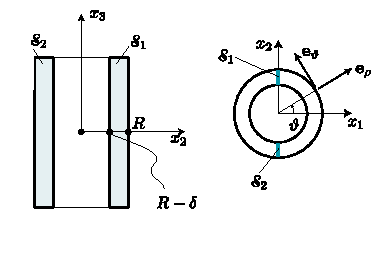
\includegraphics[scale=1.2]{figure/equilibrio/esempio13d_1}
			\end{center}
			We find that
			\begin{equation}
				\Tb \eb_1=2\sigma \sin^2\vartheta \eb_1-2\sigma\sin\vartheta\cos\vartheta\eb_2-\frac{\tau}{R}\rho \sin\vartheta\eb_3.
			\end{equation}
			On $\Sc_1$ we have $\vartheta=\pi/2$, so
			\begin{equation}
				\tb_1=\Tb \eb_1|_{\vartheta=\pi/2}=2\sigma\eb_1-\frac{\tau}{R}\rho \eb_3,
			\end{equation}
			while on $\Sc_2$ we have $\vartheta=-\pi/2$, so
			\begin{equation}
				\tb_2=\Tb \eb_1|_{\vartheta=-\pi/2}=2\sigma\eb_1+\frac{\tau}{R}\rho \eb_3.
			\end{equation}
			The resultant is then
			\begin{equation}
				\rb=\int_{-L/2}^{L/2}\int_{R-\delta}^{R}\tb_{1}+\tb_{2}=4\sigma \delta L \eb_1.
			\end{equation}
			To calculate the resultant moment with respect to the origin, we need to determine the lever arm: the position of the generic point is
			\begin{equation}
				\yb=\rho\cos\vartheta\eb_1+\rho \sin\vartheta\eb_2+y_3\eb_{3},
			\end{equation}
			on $\Sc_1$ we have
			\begin{equation}
				\yb_1 = \rho\, \eb_2+y_3\,\eb_3,
			\end{equation}
			while on $\Sc_1$ we have
			\begin{equation}
				\yb_2= -\rho\, \eb_2+y_3\,\eb_3.
			\end{equation}
			The resultant moment is then
			\begin{equation}
				\mb_0=\int_{-L/2}^{L/2}\int_{R-\delta}^R\yb_1\times \tb_1+\yb_2\times \tb_2=-\frac23 \frac{\tau}{R}(R^3-(R-\delta)^3)\,\eb_1.
			\end{equation}
		\end{enumerate}
	\end{svolgimento}
\end{exercise}

\begin{exercise}
	Let $\bar\Tb$ be the average stress in a configuration $\Omega$ subjected to volume forces $\bb$ and contact forces $\sb$ in equilibrium. Using the divergence theorem, prove that
	\begin{equation}
		\bar\Tb=\frac{1}{\textrm{vol}(\Omega)}\left( \int_{\Omega}\yb\otimes\bb+\int_{\partial\Omega}\yb\otimes\sb \right),
	\end{equation}
	where $\yb$ is the generic point in $\Omega$.
	\begin{svolgimento}
		First, observe that
		\begin{equation}
			\int_{\partial\Omega}\yb\otimes \sb=\int_{\partial\Omega}\yb\otimes \Tb \nb,
		\end{equation}
		on which we apply the divergence theorem. Working component-wise. Given a vector $\ab\in \Vc$ and a tensor $\Ab \in \Lin$,
		\begin{equation}
			(\ab \otimes \Ab \nb)_{ij}=a_i A_{jk}n_k
		\end{equation}
		and thus, by the divergence theorem
		\begin{equation}
			\int_{\partial\Omega}a_i A_{jk}n_k=\int_{\Omega}(a_i A_{jk}),_{k}.
		\end{equation}
		We have that 
		\begin{equation}
			(a_i A_{jk}),_{k}=a_{i,k}A_{jk}+a_i A_{jk,k}=\big((\grad \ab)\, \Ab^\top\big)_{ij}+(\ab \otimes \dive \Ab)_{ij}
		\end{equation}
		and thus
		\begin{equation}
			\int_{\partial\Omega}\ab \otimes \Ab \nb =\int_{\Omega}(\grad \ab)\, \Ab^\top+\ab \otimes \dive \Ab.
		\end{equation}
		Using this general result with $\ab=\yb$ and $\Ab =\Tb$:
		\begin{equation}
			\int_{\partial\Omega}\yb \otimes \Tb \nb =\int_{\Omega}(\grad \yb)\, \Tb^\top+\yb \otimes \dive \Ab=\int_{\Omega}\Tb -\yb \otimes \bb,
		\end{equation}
		from which it follows immediately that
		\begin{equation}
			\int_{\Omega}\yb \otimes \bb +\int_{\partial \Omega}\yb \otimes\sb=\int_{\Omega}\Tb,
		\end{equation}
		and thus the desired result is immediately obtained.
	\end{svolgimento}
\end{exercise}
\end{comment}

%
%\section{Principal Stresses}
%The stress vector recorded on a plane with normal vector $\nb$ generally has two components: one parallel to $\nb$
%\begin{equation}
%	\sigmab\coloneqq\sigma\nb \quad\sigma\coloneqq \tb(\nb) \cdot \nb
%\end{equation}
%called the \textit{normal stress}, and one perpendicular to $\nb$
%\begin{equation}
%	\taub\coloneqq \tb(\nb) -\sigmab.
%\end{equation}
%called the \textit{shear stress}. One may ask whether there are orientations for which the stress is purely normal. To answer this question, we need to solve the problem
%\begin{equation}\label{autov}
%	\tb(\nb)=\sigmab \quad  \Longleftrightarrow\quad \Tb \nb =\sigma \nb.
%\end{equation}
%Equation \eqref{autov}$_2$ shows that to answer our question, we need to solve an \textit{eigenvalue problem}. Since $\Tb$ is a symmetric tensor, we can appeal to the spectral theorem to conclude that its eigenvalues are all real and the eigenvectors are mutually orthogonal. Therefore, there exist three orientations, orthogonal to each other, where the stress is purely normal. The stress tensor can then be given the following \textit{spectral representation}:
%\begin{definition}
%	\begin{equation}
%		\mathbf{T}=\sum_{i=1}^3\lambda_i\mathbf{n}_i\otimes\mathbf{n}_i
%	\end{equation}
%\end{definition}
%where $\lambda_i$ are the (real) eigenvalues of $\Tb$ and $\nb_i$ are the corresponding (orthonormal) eigenvectors. The eigenvalues are called \textit{principal stresses}, and the eigenvectors are called \textit{principal directions}. We conventionally number the principal stresses as follows:
%\begin{equation}
%	\lambda_1\leq\lambda_2\leq\lambda_3.
%\end{equation}
%Thus, $\lambda_3$ is the maximum normal stress, and $\lambda_1$ is the minimum.
%
%The envelope of the principal directions defines three families of mutually orthogonal curves, known as \textit{isostatic lines}. Along these curves, the stresses are purely normal, and therefore, the material is simply compressed or stretched along these directions. Furthermore, these lines represent the points of maximum tension and compression.
%
%\begin{figure}[h!]
%	\centering
%	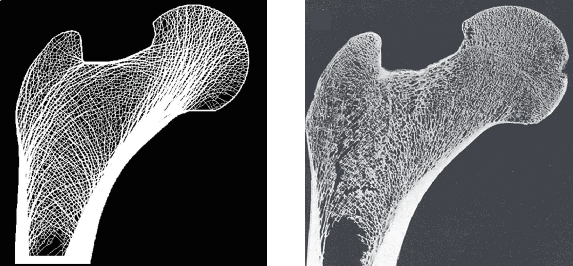
\includegraphics[width=0.8\linewidth]{figure/cinematica/osso_direzprinc}
%	\caption{Trabecular structure in a proximal femur, determined through a model (left) and actual (right). The arrangement of the trabeculae follows the isostatic lines. (Adapted from M. Huo, S. He, Y. Zhang, Y. Feng, J. Lu, Simulation on bone remodeling with stochastic nature of adult and elderly using topology optimization algorithm, Journal of Biomechanics, Volume 136, 2022.)}
%	\label{fig:ossodirezprinc}
%\end{figure}


%
%
%Nature optimizes the use of material by constructing structures that have the shape, size, and strength needed with the least possible mass. A clear example of this principle is observed in \textit{long bones}, such as the femur or humerus, where the trabeculae are arranged along the isostatic lines.
%
%The arrangement of the trabeculae along the isostatic lines had been observed long before Cauchy formally described the stress state. However, more recently, it has been shown that many living organisms can continuously model and remodel themselves in response to signals derived from the local stress state. These signals are generated by the external loads the organism must support. Taking the long bones again as an example, this adaptation process is made possible by the combined action of \textit{osteoclasts}, which break down bone tissue, and \textit{osteoblasts}, which rebuild it.
%

\section{External power, kinetic energy, inertial power}\label{kinetic}
We define \textit{external (non-inertial) power} expended on $\Pi$ as 
\begin{equation}
	\Wc^{(\rm ni)}(\Pi):=\int_{\partial\Pi}\Tb\nb\cdot\vb+\int_{\Pi}\bb^{(\rm ni)}\cdot\vb.
\end{equation}

The field
\begin{equation}
	\frac{1}{2} \rho |\vb|^2
\end{equation}
is the \textit{kinetic energy} measured per unit volume in the deformed body; hence
\begin{equation}
	K(\Pi):=\int_{\Pi}\frac{1}{2} \rho |\vb|^2
\end{equation} 
is the \textit{kinetic energy} of $\Pi$.

There is a basic relation between the kinetic-energy rate and the power expended by the inertial force $\bb^{(\rm in)}$:
\begin{equation}
	\begin{aligned}
		\left( \int_{\Pi}\frac{1}{2} \rho |\vb|^2 \right)^{\dotb}&= \frac{1}{2}\int_{\Pi}\left( \rho|\vb^2| \right)^{\dotb}+\rho|\vb|^2\dive\vb=\frac{1}{2}\int_{\Pi}\dot{\rho}|\vb|^2+\rho(|\vb|^2)^{\dotb}+\rho|\vb|^2\dive\vb\\
		&=\frac{1}{2}\int_{\Pi}\rho(|\vb|^2)^{\dotb}+|\vb|^2(\dot{\rho}+\rho\dive\vb)=\int_{\Pi}\rho\dot\vb\cdot\vb=\int_{\Pi}-\bb^{(\rm in)}\cdot\vb,
	\end{aligned}
\end{equation}
where we have made use of the mass balance; we conclude that
\begin{equation}
	\Wc^{(\rm in)}(\Pi)=-\dot K(\Pi), \qquad \Wc^{(\rm in)}(\Pi):=\int_{\Pi}\bb^{(\rm in)}\cdot\vb
\end{equation}
which means that the inertial power expenditure is balanced by the negative kinetic-energy rate of $\Pi$. As a consequence
\begin{equation}\label{bpow}
	\int_{\Pi}\bb\cdot\vb=\int_{\Pi}\bb^{(\rm ni)}\cdot\vb-\dot{\Kc}(\Pi).
\end{equation}

As to the power of contact force, we may use the divergence theorem, the identity \eqref{divid}, and the local balance equation to obtain
\begin{equation}\label{tpow}
	\int_{\partial\Pi}\Tb\nb\cdot\vb=\int_{\Pi}(\dive\Tb)\cdot\vb+\Tb\cdot\grad\vb=\int_{\Pi}\Tb\cdot\grad\vb-\bb\cdot\vb;
\end{equation}
by the symmetry of $\Tb$, we have that
\begin{equation}\label{strpow}
	\Tb\cdot\grad\vb=\Tb\cdot\Db.
\end{equation}
The right side of this latter relation establishes that the stretching $\Db$ as the appropriate power-conjugate variable for the Cauchy stress $\Tb$, and we say that $\Tb$ is power conjugate to $\Db$. The field
$$
\Tb\cdot\Db
$$
represents the power expended within $\Pi$, measured per unit volume, ad is referred as the \textit{stress power}; the integral 
\begin{equation}
	\Wc^{(\rm int)}=\int_{\Pi}\Tb\cdot\Db
\end{equation}
represents the net power expended within $\Pi$ and is referred as the internal power. Combining \eqref{bpow}, \eqref{tpow}, and \eqref{strpow}, we arrive at the power balance:
\begin{definition}
\begin{equation}\label{powerbal}
	\int_{\partial\Pi}\Tb\nb\cdot\vb+\int_{\Pi}\bb\cdot\vb=\int_{\Pi}\Tb\cdot\Db,
\end{equation}
\end{definition}
or, equivalently
\begin{equation}
	\int_{\partial\Pi}\Tb\nb\cdot\vb+\int_{\Pi}\bb^{(\rm ni)}\cdot\vb=\int_{\Pi}\Tb\cdot\Db+\dot{K}(\Pi),
\end{equation}
or rather
\begin{equation}
	\Wc^{(\rm ni)}(\Pi)=\Wc^{(\rm int)}(\Pi)+\dot{K}(\Pi).
\end{equation}
If we define as external power
\begin{equation}
	\Wc^{\rm (ext)}(\Pi)=\Wc^{(\rm ni)}(\Pi)+\Wc^{(\rm in)}(\Pi),
\end{equation}
we get
\begin{equation}
	\Wc^{\rm (ext)}(\Pi)=\Wc^{(\rm int)}(\Pi).
\end{equation}


\section{Referential form for the force balance}
When working with solids, the use a current description can be problematic; for this reason we now reformulate the basic laws in a referential setting.

Let us denote by $\Pb$ the stress measured per unit area in the reference body; it is called \textit{Piola stress}. For $\Pi \subset \Omega$, the following relation holds true:
\begin{equation}
	\int_{\fb(\partial\Pi)}\Tb\nb\dd a_{\rm cur}=\int_{\partial\Pi}\Pb\nb_{\rm ref}\dd a_{\rm ref};
\end{equation}
from \eqref{nanson} we deduce that

\begin{equation}
	\nb\dd a_{\rm cur}=(\det\Fb)\Fb^{-\top}\nb_{\rm ref}\dd a_{\rm ref}
\end{equation}

and then
\begin{equation}
	\int_{\partial\Pi}(\det\Fb)\Tb\Fb^{-\top}\nb_{\rm ref}\dd a_{\rm ref}=\int_{\partial\Pi}\Pb\nb_{\rm ref}\dd a_{\rm ref},
\end{equation}
whence
\begin{definition}
\begin{equation}\label{Pio}
	\Pb=(\det\Fb)\Tb\Fb^{-\top}.
\end{equation}
\end{definition}
The Piola stress  carries the referential vector $\nb_{\rm ref}$ to the traction $\Pb\nb_{\rm ref}$ , which is a current vector; thus, like the deformation gradient, $\Pb$ maps  the referential vector space  into the current vector space.

As to the body force, we have that
\begin{equation}
	\int_{\fb(\Pi)}\bb\dd v_{\rm cur}=\int_{\Pi}\bb_{\rm ref}\dd v_{\rm ref},
\end{equation}
whence
\begin{equation}
	\bb_{\rm ref}=(\det\Fb)\bb;
\end{equation}
it represents the  body force measured per unit volume in the reference body.

The \textit{balance of forces}, expressed referentially is then
\begin{equation}
	\int_{\partial\Pi}\Pb\nb_{\rm ref}+\int_{\Pi}\bb_{\rm ref}=\mathbf{0};
\end{equation}
on denoting by $\Div$ the referential divergence operator, it is straightforward to get the local balance of linear forces:
\begin{equation}
	\Div\Pb+\bb_{\rm ref}=\mathbf{0},
\end{equation} 
valid in the referential configuration $\Omega$
Moreover, since $\Tb=\Tb^\top$, and $\Tb=(\det\Fb)^{-1}\Pb\Fb^\top$, the balance of moments in $\Omega$ reads
\begin{equation}
	\Pb\Fb^\top=\Fb\Pb^\top.
\end{equation}


A referential version for the stress power is given by the following identity:
\begin{equation}
	\Tb\cdot\Db=\Tb\cdot\Lb=\Tb\cdot(\dot\Fb\Fb^{-1})=(\Tb\Fb^{-\top})\cdot\dot{\Fb}=(\det\Fb)^{-1}\Pb\cdot\dot{\Fb};
\end{equation}
hence
\begin{equation}\label{CaPi}
	\Tb\cdot\Db=(\det\Fb)^{-1}\Pb\cdot\dot{\Fb}.
\end{equation}
Thus
\begin{definition}
\begin{equation}
	\int_{\fb(\Pi)}\Tb\cdot\Db\dd v_{\rm cur}=\int_{\Pi}\Pb\cdot\dot{\Fb}\dd v_{\rm ref}.
\end{equation}
\end{definition}
The field $\Pb\cdot\dot{\Fb}$ represents the stress power measured per unit volume in the reference body.


\subsection{Power-conjugate pairings. Second Piola stress}
The stress power $\Tb\cdot\Db$ and $\Pb\cdot\dot{\Fb}$ are two examples of power-conjugate pairing. There is a crucial difference between $\Db$ and $\dot{\Fb}$: the former is purely a measure of the rate at which material elements stretch, while the latter carries information concerning the rates at which material elements stretch and rotate. One might therefore ask whether there are alternative referential measures of stress power in which a measure of stress is paired with a pure strain-rate.

In particular, we seek a pairing involving a measure $\Sb$ of stress that is conjugate to the time-rate $\dot{\Cb}$ of the right Cauchy-Green tensor. To determine the form of $\Sb$, we notice the following set of identities:
\begin{equation}
	\begin{aligned}
		\Tb\cdot\Db&=\frac 12 \Tb\cdot(\Lb+\Lb^\top)=\\
		&=\frac 12 \Tb\cdot(\dot{\Fb}\Fb^{-1}+\Fb^{-\top}\dot{\Fb}^\top)\\
		&=\frac 12 \Tb\cdot\Fb^{-\top}(\Fb^\top\dot{\Fb}+\dot{\Fb}^\top\Fb)\Fb^{-1}\\
		&=\frac 12 (\Fb^{-1}\Tb\Fb^{-\top})\cdot(\Fb^\top\dot{\Fb}+\dot{\Fb}^\top\Fb)\\
		&=\frac 12 (\Fb^{-1}\Tb\Fb^{-\top})\cdot\dot\Cb\\
		&=\frac 12(\det\Fb)^{-1}(\Fb^{-1}\Pb)\cdot\dot{\Cb}.
	\end{aligned}
\end{equation}
We define the \textit{second Piola stress tensor} as 
\begin{definition}
\begin{equation}
	\Sb:=\Fb^{-1}\Pb=(\det \Fb)\,\Fb^{-1}\Tb \Fb^{-\top}
\end{equation}
\end{definition}
so that
\begin{equation}
	\Tb\cdot\Db=\frac{1}{2}(\det\Fb)^{-1}\Sb\cdot\dot{\Cb}.
\end{equation}
We notice that the second Piola stress tensor is symmetric.

The Cauchy stress $\Tb$ maps $\Vcu$ into $\Vcu$; the Piola stress $\Pb$ maps $\Vr$ into $\Vcu$; the second Piola stress $\Sb$ maps $\Vr$ into $\Vr$.


In continuum mechanics, different stress tensors describe internal forces from different perspectives, depending on whether they refer to the current or reference configuration. The \emph{Cauchy stress tensor} $\Tb$ is the most physical and directly measurable one: it gives the force per unit area acting on a surface element \emph{in the deformed configuration}. That is, it tells how internal forces are transmitted across a cut in the current body. The \emph{first Piola stress tensor} \(\Pb \) represents the same actual forces, but expressed with respect to \emph{undeformed} surface elements. It thus combines current forces with reference areas, making it a mixed (and generally non-symmetric) object. Finally, the \emph{second Piola stress tensor} \( \Sb \) fully pulls the description back to the reference configuration: it expresses both forces and areas as if the body were still undeformed. This makes \(\Sb \) symmetric. In summary, \( \Tb \) lives in the deformed configuration, \(\Pb\) mixes current forces and reference areas, and \(\Sb\) lives entirely in the reference world.




\chapter{Frame indifference}\label{FI}
\section{Frame of reference}
The region $\fb_t(\Omega)$ is observed during the motion. The ambient space through which $\Omega_t$ evolves is termed the \textit{observed space}; the ambient space for the reference body is termed \textit{reference space}.

A \textit{change of frame} is defined, at each fixed time $t$, by a rotation $\Qb(t)$ and a translation $\wb(t)$ of the observed space and transforms current points to current points:
\begin{equation}\label{y+}
	\yb^+=\wb(t)+\Qb(t)\yb.
\end{equation}

We refer to $\wb(t)\in\Ecu$ as the \textit{frame translation} and $\Qb(t)\in\Rot$ as the \textit{frame rotation}. Since $\Qb\in\Rot$,
\begin{equation}
	\Qb\Qb^\top=\Ib \quad \Rightarrow\quad (\Qb\Qb^\top)^{\dotb}=\mathbf{0}, \quad \Rightarrow\quad \dot{\Qb}\Qb^\top+\Qb\dot{\Qb}^\top=\mathbf{0},
\end{equation}
and then then
\begin{equation}
	\Omegab:=\dot{\Qb}\Qb^\top\in\Skw,
\end{equation}
and it is called frame-spin; $\Omegab$ represents  the rate at which the new frame is spinning. It is worth noticing that a change of frame does not affect the reference space and then reference points and reference vectors are \textit{invariant} under changes in frame; moreover scalar fields such as the density are invariant: $\rho^+=\rho$.

\subsection{Frame-indifferent fields}
A vector field is \textit{frame-indifferent} if it simply rotates with the frame rotation:
\begin{equation}
	\gb^+=\Qb\gb.
\end{equation}
A tensor field $\Gb$ is frame indifferent if, given indifferent vector fileds $\hb$ and $\gb$, with $\gb$ arbitrary, and any change in frame,
\begin{equation}
	\hb=\Gb\gb \quad {\rm implies} \quad \hb^+=\Gb^+\gb^+.
\end{equation}
Now, if $\hb=\Gb\gb$ it follows that
\begin{equation}
	\hb^+=\Qb\hb=\Qb\Gb\gb=\Qb\Gb\Qb^\top\gb^+,
\end{equation}
where we have used the fact that $\gb=\Qb^\top\gb^+$. We then conclude that
\begin{equation}
	\Gb^+=\Qb\Gb\Qb^\top.
\end{equation}

\subsection{Transformation rules for kinematic fields}
Since $\yb=\fb(\xb,t)$ is a current point, but $\xb$ is referential, eq. \eqref{y+} implies
\begin{equation}
	\fb^+(\xb,t)=\wb(t)+\Qb(t)\, \fb(\xb,t) .
\end{equation}
On taking the gradient with respect to $\xb$, we get
\begin{equation}
	\Fb^+(\xb,t)=\Qb(t)\Fb(\xb,t).
\end{equation}
From this relation we get:
\begin{equation}
	\Cb^+=(\Fb^+)^\top\Fb^+=\Fb^\top \Qb \Qb \Fb=\Fb^\top\Fb \quad \Rightarrow \quad \Cb^+=\Cb.
\end{equation}
Then the fields $\Cb$, $\Ub$, $\Eb$ are \textit{invariant}.
On recalling that $\Rb=\Fb\Ub^{-1}$ and $\Fb^+=\Qb\Fb$, we conclude that
\begin{equation}
	\Rb^+=\Qb\Fb\Ub^{-1}=\Qb\Rb.
\end{equation}



As to the velocity gradient, we get
\begin{equation}\label{Lb+}
	\Lb^+=(\Fb^+)^{\mathop{\vcenter{\hbox{\Large$\cdot$}}}}(\Fb^+)^{-1}=(\Qb\dot\Fb+\dot\Qb\Fb)(\Fb^{-1}\Qb^{-1})=\Qb \dot\Fb\Fb^{-1}\Qb^\top+\dot\Qb\Qb^\top=\Qb\Lb\Qb^\top+\Omegab.
\end{equation}

In summary:
\begin{definition}
\begin{equation}
	\begin{aligned}
		&\Fb^+=\Qb\Fb,\\
		&\Rb^+=\Qb\Rb,\\
		&\Ub^+=\Ub,\\
		&\Cb^+=\Cb,\\
		&\Eb_{\rm G}^+=\Eb_{\rm G},\\
		&\Vb^+=\Qb\Vb\Qb^\top,\\
		&\Bb^+=\Qb\Bb\Qb^\top,\\
		& \Lb^+=\Qb\Lb\Qb^\top+\Omegab.
	\end{aligned}
\end{equation}
\end{definition}
In other words:
\begin{itemize}
	\item the tensors $\Vb$ and $\Bb$ are \textit{frame-indifferent};
	\item the tensors $\Ub$, $\Cb$, $\Eb_{\rm G}$ are \textit{invariant};
	\item the tensors $\Fb$, $\Lb$ and $\Rb$ are neither frame-indifferent nor invariant.
\end{itemize}


\section{Frame-indifference principle}
A basic principle underlying most of physics is that
\begin{itemize}
	\item \emph{physical laws be independent of the frame of reference},
\end{itemize}
which is the frame-indifference principle.

\subsection{Transformation rules for stress and body force}
We assume that the balance of forces is frame-indifferent:
\begin{equation}
	\int_{\partial\Pi_t^+}\Tb^+\nb^++\int_{\Pi_t^+}\bb^+=\mathbf{0},
\end{equation}
where $\Pi_t^+=\fb^+(\Pi,t)$ is the deformed region $\Pi_t$ as viewed with respect to the new frame. The mapping $\tb(\nb)=\Tb\nb$ carries current vectors $\nb$ to current vectors $\tb$. We assume that
\begin{equation}
	\tb^+=\Qb\tb, \quad \nb^+=\Qb\nb.
\end{equation}
It follows that
\begin{equation}
	\tb^+=\Tb^+\nb^+ \quad \Rightarrow\quad \Qb\tb=\Tb^+\Qb\nb  \quad \Rightarrow\quad \tb=(\Qb^\top\Tb^+\Qb)\nb=\Tb\nb,
\end{equation}
which allows to conclude that
\begin{definition}
	\begin{equation}
	\Tb^+=\Qb\Tb\Qb^\top;
\end{equation}
\end{definition}
then the \textit{Cauchy stress is frame indifferent}.
Since
\begin{equation}
	\int_{\partial\Pi_t^+}\Tb^+\nb^+=\int_{\partial\Pi_t}(\Qb\Tb\Qb^\top)\Qb\nb=\Qb\int_{\partial\Pi_t}\Tb\nb,
\end{equation}
we conclude that
\begin{equation}
	\int_{\Pi_t^+}\bb^+=\Qb\int_{\partial\Pi_t}\Tb\nb=\Qb\bb;
\end{equation}
thus the \textit{body force is frame indifferent}.









\chapter{Principle of Virtual Powers}\label{PPV}

In mechanics, there are two distinct ways to provide a mathematical representation of the concept of force. The first is to represent it as an \textit{applied vector}, a mathematical entity characterized by an origin, magnitude, direction, and sense. Its natural extension to continuous media leads to the definition of vector fields associated with measures, hence giving rise to `body forces', `surface forces', `forces per unit mass', and so on.

The second approach, which dates back at least to d'Alembert, is what is commonly referred to as the \textit{principle of virtual power}. This second method is in fact more natural than the first, as it mathematically formalizes what is typically done in practice to evaluate a force. For example, if one wants to assess the weight of an object, the most natural operation is to `weigh' it --- that is, to apply a velocity and gauge the effort required to do so. Our brain cannot directly perceive a force, but only the power it expends.

From a mathematical standpoint, this procedure can be described as follows: at a given instant, a virtual velocity field \( \tilde\vb \) is considered on the system \( \Pi \); the forces producing this motion are known if their \textit{virtual power} is known. More precisely --- and more abstractly --- one considers a set  of virtual velocities \( \tilde\vb \), and the forces acting on the system are said to be known if there exists a linear functional \( \mathcal{W}(\Pi)[\tilde\vb] \) whose value, for every \( \tilde\vb \), equals the virtual power produced by the forces during the motion defined by \( \tilde\vb \).

The core idea underlying this second viewpoint is that of \textit{duality}. One of its main advantages lies in the flexibility it offers in defining the space of virtual velocities, allowing for a more or less refined description of the system's motion.  It must be acknowledged that the notion of a linear functional defined on a vector space is more abstract and mathematically involved than that of a vector field, which explains why the first description of force historically prevailed, at least initially. Furthermore, when this idea first emerged, the concept of duality --- which can be seen as a precursor to the modern notions of \textit{measure} and \textit{distribution} --- had not yet been fully developed. Today, functional analysis and its applications to mechanics have provided powerful mathematical tools for the notion of duality, and since at least the mid-20th century, the use of concepts related to virtual power and duality has proven extremely fruitful in the development of field theories.


In this chapter we rederive the balance laws for force and moment. Unlike traditional treatments, we do not take these laws as starting assumptions. Instead, we show how they can be deduced from more basic premises. In the same spirit, we do not assume the validity of Cauchy’s formula $\tb(\nb)=\Tb \nb$.

\section{Principle of Virtual Power}
Our starting point is the generalized power balance \eqref{powerbal}, written in a more general form that avoids invoking Cauchy’s theorem:
\begin{equation}\label{powerbal1}
\int_{\partial \Pi}\tb(\nb)\cdot \vb+\int_\Pi \bb\cdot\vb=\int_\Pi \Tb \cdot \grad \vb.
\end{equation}
The defining feature of \eqref{powerbal1} is that it incorporates the Cauchy stress via its internal power expenditure, without assuming symmetry or frame indifference.

We reinterpret the power balance  \eqref{powerbal1} by replacing the actual velocity $\vb$ with a virtual field $\tilde{\vb}$, not connected to the real motion. Time $t$ is held fixed, so $\tilde{\vb}$  is treated as an arbitrary function, and $\Pi$ as any subregion of the deformed body $\widetilde{\Omega}$.

On denoting by
\begin{equation}
\Wc^{\rm (ext)}(\Pi)[\tilde{\vb}]=\int_{\partial \Pi}\tb(\nb)\cdot \tilde\vb+\int_\Pi \bb\cdot\tilde\vb, \qquad \Wc^{\rm (int)}(\Pi)[\tilde{\vb}]=\int_\Pi \Tb \cdot \grad \tilde\vb
\end{equation}
the esternal and internal virtual power, we rewrite  \eqref{powerbal1} in the form of a 
\begin{definition}
\textbf{Virtual Power Balance}
\begin{equation}\label{VPB}
\int_{\partial \Pi}\tb(\nb)\cdot \tilde\vb+\int_\Pi \bb\cdot\tilde\vb=\int_\Pi \Tb \cdot \grad \tilde\vb.
\end{equation}
\end{definition}

\section{Force balance, stress}
We now show that the \eqref{VPB} encapsulates the local force balance and the Cauchy theorem.   Assume that \eqref{VPB} is satisfied for all $\Pi$ and $\tilde\vb$. Then, using the divergence theorem, we get
\begin{equation}
\int_\Pi\Tb \cdot \grad \tilde\vb=\int_{\partial\Pi}\Tb\cdot\tilde\vb-\int_\Pi\dive \Tb \cdot \tilde\vb,
\end{equation}
ant then, by  \eqref{VPB},
\begin{equation}
\int_\Pi (\dive\Tb +\bb)\cdot \tilde \vb +\int_{\partial\Pi}(\tb(\nb)-\Tb\nb)\cdot \tilde \vb=0,
\end{equation}
for every choice of the field $\tilde\vb$. We appeal to the 
\begin{definition}
\textbf{Fundamental Lemma  of the Calculus of Variations}: Let $\fb$ be a continuous vector field on $\Pi$, let $\hb$ be a continuous vector field on a smooth subsurface $\Sigma$ of $\partial\Pi$, and assume that
\begin{equation}
\int_{\Pi}\fb\cdot\bm{\phi}+\int_{\Sigma}\hb\cdot\bm{\phi}=0
\end{equation}
for all continuous vector fields $\bm{\phi}$ on $\Pi$, that vanishes on $\partial\Pi\setminus\Sigma$. Then
\begin{equation}
\fb=\mathbf{0} \quad \textrm{in $\Pi$}, \qquad \hb=\mathbf{0}\quad \textrm{in $\Sigma$}.
\end{equation}
\end{definition}
This lemma, with $\Sigma=\partial\Pi$ and $\bm{\phi}=\tilde\vb$ allows to  conclude that
\begin{equation}
\dive\Tb +\bb=\mathbf{0}
\end{equation}
in $\Pi$ and 
\begin{equation}
\tb(\nb)=\Tb\nb
\end{equation}
on $\partial\Pi$. Since $\Pi$ is arbitrary, these relations must hold throughout $\widetilde{\Omega}$.


\section{Symmetry and frame-indifference}\label{symPVP}
We now show that the requirement that the internal virtual power $ \Wc^{\rm (int)}(\Pi)[\tilde{\vb}]$ be invariant under changes of frame implies that $\Tb$ is symmetric and frame-indifferent.
Assuming time is fixed and omitted, we introduce an arbitrary frame change represented by the mapping $\bm{\phi}$, which takes  points $\yb$ to $\yb^+$, in accordance with \eqref{y+}; namely,
\begin{equation}\label{yb+}
	\yb^+=\bm{\phi}(\yb)=\wb+\Qb\,\yb,
\end{equation}
with $\Qb$ the frame rotation.  To facilitate the discussion of how the internal power transforms, it is helpful to keep the spatial arguments explicit. For this reason, we express the internal power in the following way:
\begin{equation}
 \Wc^{\rm (int)}(\Pi)[\tilde{\vb}]=\int_\Pi\Tb(\yb) \cdot \grad \tilde\vb(\yb).
\end{equation}
The virtual velocity gradient $\tilde\Lb(\yb)=\grad\tilde\vb(\yb)$ transforms under the change of frame as \eqref{Lb+}:
\begin{equation}\label{L+v}
\tilde\Lb(\yb^+)=\Qb \tilde\Lb(\yb)\Qb^\top+\Omegab.
\end{equation}
The frame-indifference then requires that
\begin{equation}\label{FRIT}
\int_{\Pi}\Tb(\yb)\cdot \tilde\Lb(\yb)\,\dd v(\yb)=\int_{\Pi^+}\Tb^{+}(\yb^+)\cdot\tilde\Lb^+(\yb^+)\,\dd v(\yb^+).
\end{equation}
On using \eqref{yb+} and \eqref{L+v}, we can write the RHS as 
\begin{equation}
\int_{\Pi^+}\Tb^{+}(\yb^+)\cdot\tilde\Lb(\yb^+)\,\dd v(\yb^+)=\int_{\Pi^+}\Tb^{+}(\yb^+)\cdot\Big(  \Qb \tilde\Lb(\bm{\phi}^{-1}(\yb^+)\Qb^\top+\Omegab\Big)  \,\dd v(\yb^+).
\end{equation}
Since the Jacobian of the transformation $\bm{\phi}$ satisfies $\det\grad \bm{\phi}=\det\Qb=1$, if we change the variable of integration from $\yb^+$ to $\yb$ we find that
\begin{equation}
	\int_{\Pi^+}\Tb^{+}(\yb^+)\cdot\tilde\Lb(\yb^+)\,\dd v(\yb^+)=\int_{\Pi}\Tb^{+}(\bm{\phi}(\yb))\cdot\Big(  \Qb \tilde\Lb(\yb)\Qb^\top+\Omegab\Big)  \,\dd v(\yb).
\end{equation}
Therefore, the frame indifference requirement \eqref{FRIT} implies
\begin{equation}
	\int_{\Pi}\Tb(\yb)\cdot \tilde\Lb(\yb)\,\dd v(\yb)=\int_{\Pi}\Tb^{+}(\bm{\phi}(\yb))\cdot\Big(  \Qb \tilde\Lb(\yb)\Qb^\top+\Omegab\Big)  \,\dd v(\yb).
\end{equation}
or, equivalently, since the region $\Pi$ is arbitrary
\begin{equation}
\Tb\cdot\tilde\Lb=\Tb^+\cdot (\Qb \tilde\Lb \Qb^\top+\Omegab)=(\Qb^\top\Tb^+\Qb)\cdot\tilde\Lb+\Tb^+\cdot\Omegab,
\end{equation}
where we have suppressed arguments.

Let us consider a change of frame in which $\Qb$ is constant. We therefore have that
\begin{equation}
(\Tb-\Qb^\top\Tb^+\Qb)\cdot\tilde\Lb=0,
\end{equation}
for all choices of $\tilde\Lb$, and then
\begin{equation}
	\Tb^+=\Qb\Tb\Qb^\top.
\end{equation}
The Cauchy stress is therefore frame-indifferent. With this, we find that
\begin{equation}
\Tb^+\cdot\Omegab=0;
\end{equation}
on the other hand,  we may assume that $\Omegab$ is an arbitrary skew-symmetric tensor; thus $\Tb^+=(\Tb^+)^\top$, and then
\begin{equation}
	\Tb=\Tb^\top;
\end{equation}
the Cauchy stress is therefore symmetric.

The preceding results highlight the broad applicability of the principle of virtual power. Its significance becomes especially evident in nonclassical contexts where additional kinematical degrees of freedom are present. Notably, we will make repeated use of this principle in our discussion of plasticity.

\begin{remark}
One often finds this principle formulated \textit{erroneously} in terms of an underlying free energy, an error
arising from the observation that — in the absence of dissipation — energy minimization generally
results in partial-differential equations equivalent to those resulting from a corresponding virtual-power principle.

\end{remark}




\chapter{Energy Balance and Entropy Imbalance}

In addition to the balance laws for forces, the response of a body is governed by  
\begin{itemize}
	\item[(i)] the energy balance law, and  
	\item[(ii)] an entropy imbalance law.
\end{itemize}

These two laws are known as the \textit{first} and \textit{second laws of thermodynamics}. As we did for the balance of forces and moments, we will first formulate these laws in a global form for parts \( \Pi \), and then, by invoking the requirement that the underlying parts be arbitrary and applying the localization lemma, we will derive local forms of the laws in the form of partial differential equations and inequalities.



\section{Energy Balance: First Law of Thermodynamics}
We define \textit{motion} as a one-parameter family of deformations:
\[
\mathcal{M} = \left\{ \fb_t \mid t \in T \subset \mathbb{R} \right\}, \qquad 	(\xb, t) \mapsto \yb = \fb(\xb, t) = \fb_t(x);
\]
where the parameter \( t \) typically represents \textit{time}. In a motion, we can define the \textit{velocity}
\[
\mathbf{v}(\xb) = \partial_t \yb = \partial_t \fb(\xb, t)= \partial_t \ub(\xb, t).
\]

A pair consisting of \( \Mc \) and a symmetric tensor field \( \Tb \), with \( T(\cdot, t) \) smooth for each \( t \in T \), is called a \textit{dynamic process}.

In addition to describing the motion and the associated stress, we will be interested in describing the evolution of a material system in terms of its thermal and mechanical states, analyzing a \textit{thermodynamic process}, in which we will consider not only stress and deformation, but also quantities like temperature, internal energy, entropy, and heat flux.

Let us now look at the laws that govern thermodynamic processes.

The \textit{first law of thermodynamics} represents a balance between the rate of change of internal energy and the rate at which energy is transferred, in the form of heat, to a part \( \Pi \) plus the mechanical power spent. %In the following, we will limit ourselves to considering small deformations.

We introduce the \textit{internal energy} \( E(\Pi) \) of part \( \Pi \), expressed in terms of an internal energy density per unit volume \( \varepsilon \):
\begin{equation}
	E(\Pi) = \int_{\Pi}\rho \varepsilon.
\end{equation}

Its time derivative, denoted as \( \dot{E}(\Pi) \), represents the rate of energy supply to part \( \Pi \).

The sum of the internal energy and the kinetic energy delivers the \textit{total energy}.

We consider two types of energy input:

\begin{enumerate}
	\item \textit{Mechanical Sources}. The force system acting on \( \Pi \), due to the fact that the points of \( \Pi \) assume a certain velocity during the motion, expends power. In particular, we define the \textit{power of the forces} acting on \( \Pi \), or \textit{external power}, as the quantity
	\begin{equation}\label{Wext}
		\Wc^{\rm ext}(\Pi)= \int_{\Pi} \bb \cdot \vb + \int_{\partial \Pi} \tb\cdot \vb.
	\end{equation}
	
	The first contribution is the power spent by volume forces, while the second is the power spent by the tensions acting on the boundary of \( \Pi \), which we now assume to be entirely internal to \( \Omega \).
	
	Using Cauchy's theorem, we can write that 
	\begin{equation}
		\Wc^{\rm ext}(\Pi)=	\int_{\Pi} \bb \cdot \vb + \int_{\partial \Pi} \Tb \nb\cdot \vb = \int_{\Pi} \bb \cdot \vb + \int_{\Pi} \dive(\Tb^\top\vb);
	\end{equation}
	using the identity \eqref{identitadiff}$_5$ and recalling that \( \Tb \in \Sym \), we obtain that 
	\begin{equation}
		\Wc^{\rm ext}(\Pi)	= \int_{\Pi} (\dive\Tb+\bb) \cdot \vb +  \Tb \cdot \Db.
	\end{equation}
%	where we have denoted by
%	\begin{equation}
%		\dot\Eb=\sym \grad \dot \ub=\sym \grad \vb
%	\end{equation}
%	the \textit{strain rate}.
	
	 Recalling that, for the pointwise equilibrium equation \( \dive\Tb+\bb=\mathbf{0} \), we conclude that
	\begin{equation}
		\Wc^{\rm ext}(\Pi)= \int_{\Pi}  \Tb \cdot \Db=	\Wc^{\rm int}(\Pi),
	\end{equation}
	where \( \Wc^{\rm int}(\Pi) \) denotes the \textit{internal power}, or \textit{stress power}. We have thus concluded that the external power equals the stress power.
	
	\item \textit{Thermal Sources}. We denote the \textit{heat transfer} to part \( \Pi \) as \( \Qc(\Pi) \), which consists of two contributions: one from the \textit{heat flux} \( \qb \) transferred to \( \Pi \) through its boundary \( \partial\Pi \), and an \textit{internal heat source} \( r \) (generated, for example, by chemical reactions, radiation, etc):
	\begin{equation}
		\Qc(\Pi) = -\int_{\partial \Pi} \qb\cdot \mathbf{n} + \int_{\Pi}\rho r.
	\end{equation}
	The negative sign in the first contribution is due to the fact that, since \( \nb \) is the outward normal at \( \partial\Pi \), we require that the heat transfer be non-negative when the flux is entering \( \partial\Pi \).
	
%	\begin{remark}
%		The physical dimensions of the heat flux and the internal heat source are respectively
%		\begin{equation}
%			[\qb]=\left[\frac{{\rm energy}}{{\rm time}\times{\rm area}} \right], \qquad [r]=\left[\frac{{\rm energy}}{{\rm time}\times{\rm volume}} \right]
%		\end{equation}
%	\end{remark}
	
	Using the divergence theorem, the heat transfer \( \Qc (\Pi) \) can be rewritten as
	\begin{equation}
		\Qc(\Pi)= \int_{\Pi}(-\dive \qb +\rho r).
	\end{equation}
	
\end{enumerate}


At this point, we can establish that the energy balance corresponds to the following relation:
\begin{equation}
	\dot{E}(\Pi)=\Wc^{\rm int}(\Pi)+\Qc (\Pi),
\end{equation}
or
\begin{equation}
	\left(  \int_{\Pi}\rho \varepsilon\right)^{\mathop{\vcenter{\hbox{\Large$\cdot$}}}}= \int_{\Pi} \Tb \cdot \Db - \dive \, \mathbf{q} + \rho  r.
\end{equation}
By the Reynolds' theorem \eqref{reyn} and the  mass \eqref{masbal}, we have that
Since \( \Pi \) does not depend on time, we can thus establish that 
\begin{equation}
	\left( \int_{\Pi}\rho\varepsilon \right)^{\dotb}=\int_{\Pi}\rho\dot\varepsilon,
\end{equation}
and therefore 
\begin{equation}
	\int_{\Pi}\rho \dot{\varepsilon}= \int_{\Pi}  \Tb \cdot \Db - \dive \, \mathbf{q} + r.
\end{equation}
Using the usual localization lemma, we then obtain the following

\begin{definition}
	\textit{\textbf{Local energy balance equation}}:
	\begin{equation}\label{bilen}
	\rho	\dot{\varepsilon} =\Tb \cdot \Db - \dive \, \mathbf{q} + \rho r.
	\end{equation}
\end{definition}





\section{Entropy Imbalance: Second Law of Thermodynamics}

The power expenditure represents a macroscopic transfer of energy, as it is calculated using the velocity of material points. We consider heat as an additional form of energy transfer due to the \textit{fluctuations} of atoms and/or molecules, and \textit{entropy} as a measure of the disorder in the system induced by these fluctuations: the greater the degree of disorder, the higher the entropy. Like energy, regions of the body possess entropy, and entropy can flow from one region to another and also from a region to the external world. However, unlike energy, parts of the body are allowed to \textit{produce} entropy.

We introduce the \textit{internal production of entropy} of the part $\Pi$
\begin{equation}
	\Delta (\Pi)=\int_{\Pi}\rho\delta,
\end{equation}
where $\delta$ represents the density of entropy production. We assume that this production has two contributions:
\begin{equation}
	\Delta(\Pi)= \dot{\Hc}(\Pi)-\Dc(\Pi);
\end{equation}
where $\dot{\Hc}(\Pi)$ represents the rate at which the entropy of $\Pi$ increases, and $\Dc(\Pi)$ is the rate at which entropy is transferred to $\Pi$.

The fundamental premise that systems tend to increase their degree of disorder is reflected in the requirement that the internal production of entropy be non-negative in every region $\Pi$:
\begin{equation}
	\Delta(\Pi)\geq 0.
\end{equation}

As with energy, we assume that there exists a scalar field $\eta$, the \textit{entropy density}, such that
\begin{equation}
	\Hc(\Pi)=\int_{\Pi}\rho\eta.
\end{equation}
In analogy with heat transfer, we assume that the entropy contribution is characterized by a flux $\hb$ and a source $s$:
\begin{equation}
	\Dc(\Pi)=-\int_{\partial\Pi}\hb \cdot \nb +\int_{\Pi} \rho s,
\end{equation}
from which we obtain
\begin{equation}\label{sbentr}
	\left( \int_{\Pi}\rho\eta \right)^{\mathop{\vcenter{\hbox{\Large$\cdot$}}}}\geq -\int_{\partial\Pi}\hb \cdot \nb +\int_{\Pi} \rho s,
\end{equation}
which represents the form we give to the second law of thermodynamics in this context.

\begin{remark}
	The theory we are developing is consistent with two famous statements by \textsc{Rudolph Clausius}:
	\begin{itemize}
		\item \textit{Die Energie des Weltalls ist konstant } (The energy of the universe is constant).
		\item \textit{Die Entropie des Weltalls strebt einem Maximum zu} (The entropy of the universe tends to a maximum).
	\end{itemize}
	The word \textit{Weltall} can be more prosaically replaced with an isolated system, that is, a system for which $\qb \cdot \nb = \hb \cdot \nb = 0$ and $r = s = 0$; in this case, the energy balance and the entropy imbalance reduce to
	\begin{equation}
		\left(\int_{\Pi}\varepsilon\right)^{\mathop{\vcenter{\hbox{\Large$\cdot$}}}}=0, \qquad \left( \int_{\Pi}\eta \right)^{\mathop{\vcenter{\hbox{\Large$\cdot$}}}}\geq 0,
	\end{equation}
	which correspond to Clausius' two statements.
\end{remark}

A fundamental hypothesis of the theory relates the entropy and heat fluxes and the two sources; in particular, it is assumed that there exists a scalar field $\vartheta>0$, the \textit{absolute temperature}, such that
\begin{equation}
	\hb =\frac{\qb}{\vartheta}, \qquad s=\frac{r}{\vartheta}.
\end{equation}

The entropy flux and heat flux have the same direction, and one cannot vanish without the other. This hypothesis reflects the fact that a heat flux has different entropic effects depending on the temperature at which it occurs; in particular, heat received at low temperatures is more ``effective'' than that received at high temperatures.

We can then write the entropy imbalance \eqref{sbentr} in the form of the

\begin{definition}
	\noindent \textbf{\textit{Clausius-Duhem Inequality}}:
	\begin{equation}
		\left( \int_{\Pi}\rho\eta \right)^{\mathop{\vcenter{\hbox{\Large$\cdot$}}}}\geq -\int_{\partial\Pi}\frac{\qb}{\vartheta} \cdot \nb +\int_{\Pi} \frac{\rho r}{\vartheta}.
	\end{equation}
\end{definition}

Using the usual localization lemma, we obtain the 
\begin{definition}
	\textbf{\textit{Local Entropy Imbalance Inequality}}:
	\begin{equation}
	\rho	\dot \eta \geq -\dive \left( \frac{\qb}{\vartheta} \right)+\frac{\rho r}{\vartheta}
	\end{equation}
\end{definition}
and the expression for the internal entropy production density
\begin{equation}\label{delta}
\rho	\delta=\rho \dot{\eta}+\dive \left( \frac{\qb}{\vartheta} \right)-\frac{\rho r}{\vartheta}\geq 0.
\end{equation}

When irreversible processes occur within a system, such as heat conduction, there is internal entropy production $\delta$, which measures the rate of entropy generated per unit volume due to these irreversible processes. We have seen how the absolute temperature $\vartheta$ serves as a scaling factor that converts entropy production into dissipated energy. The quantity
\begin{equation}
	\gamma\coloneqq\delta\vartheta
\end{equation}
represents the \textit{rate of energy dissipation} (or \textit{dissipated power}) per unit volume in the system. In fact, in a thermodynamic system, the second law of thermodynamics establishes that entropy production is always associated with a loss of available energy: this loss manifests itself as internal energy dissipation.

Using \eqref{delta}, we can write the dissipated power as
\begin{equation}
\rho	\gamma=\rho \vartheta\dot\eta+\vartheta\dive \left( \frac{\qb}{\vartheta} \right)-\rho r\geq 0.
\end{equation}

Using identity \eqref{identitadiff}$_3$, we can deduce that
\begin{equation}
	\dive \left( \frac{\qb}{\vartheta} \right)=\grad\left(\frac{1}{\vartheta}\right)\cdot\qb +\frac{1}{\vartheta}\dive \qb =-\frac{1}{\vartheta^2}\grad\vartheta\cdot \qb +\frac{1}{\vartheta}\dive \qb 
\end{equation}
and therefore
\begin{equation}\label{disga}
\rho	\gamma=\rho \vartheta\dot\eta-\frac{1}{\vartheta}\grad\vartheta\cdot \qb +\dive \qb -\rho r\geq 0.
\end{equation}

Using the local energy balance equation \eqref{bilen}, we can establish that
\begin{equation}
	\rho\gamma=\rho\vartheta\dot\eta-\frac{1}{\vartheta}\grad\vartheta\cdot \qb +\Tb \cdot\Db-\rho \dot{\varepsilon}\geq 0. 
\end{equation}
If the quantity $\rho\gamma=\rho\delta\vartheta$ represents the dissipated power per unit volume, i.e., the density of energy converted into heat and increasing the entropy of the system due to irreversible processes, we can interpret the quantity $\rho\vartheta\eta$ as the energy density ``trapped'' in the entropy of the system. 
The difference between the total energy density $\varepsilon$ and the ``trapped'' energy in entropy represents the energy available to the system. Thus, we introduce the \textit{Helmholtz free energy} per unit volume
\begin{equation}
	\psi=\varepsilon-\vartheta\eta.
\end{equation}

Thus \eqref{disga} can then be rewritten as the
\begin{definition}
	\textbf{\textit{Reduced Dissipation Inequality}}:
	\begin{equation}\label{DDR}
		-\rho\gamma=\rho(\dot{\psi}+\eta \dot{\vartheta})-\Tb\cdot\Db+\frac{1}{\vartheta}\qb \cdot \grad \vartheta\leq 0.
	\end{equation}
\end{definition} 
The terms in \eqref{DDR} have the dimensions of (energy)/time. Integrating over part $\Pi$, we can interpret the various terms:
\begin{equation}
	\underbrace{\int_{\Pi}\rho\gamma}_{{\rm dissipation}\geq 0}=\underbrace{\int_{\partial \Pi}\Tb \nb \cdot \vb +\int_{\Pi}\bb\cdot \vb}_{{\rm external\; power}}-
	\underbrace{\left(\int_{\Pi}\rho\psi\right)^{\mathop{\vcenter{\hbox{\Large$\cdot$}}}}}_{\scriptsize \shortstack{\text{rate of change} \\ \text{of the free energy}}}
	-\underbrace{\int_{\Pi}\rho\eta \dot{\vartheta}+\frac{1}{\vartheta}\qb \cdot \grad\vartheta}_{\text{thermal energy}}
\end{equation}

Let’s further detail the meaning of the last contribution, thermal energy. Entropy $\eta$ is associated with the energy ``stored'' thermally in the system. At higher temperatures, each unit of entropy corresponds to a greater amount of thermal energy. When the temperature changes with time $\dot{\vartheta}$, the thermal energy associated with this entropy also changes. In other words, the term $\eta\dot{\vartheta}$ represents the thermal energy per unit volume that is added or removed from the system due to the change in temperature. If $\dot{\vartheta}$ is positive, the temperature increases, and the system gains thermal energy; if $\dot{\vartheta}$ is negative, the system loses thermal energy.

The second term concerns the heat flux $\qb$ and the temperature gradient $\grad\vartheta$. The quantity $\frac{1}{\vartheta}\qb \cdot \grad\vartheta$ represents the internal dissipation associated with heat conduction. Specifically, $\qb \cdot \grad\vartheta$ describes how much heat flows through the system in the presence of a temperature gradient; dividing by $\vartheta$, we obtain a quantity proportional to the generation or absorption of entropy associated with this heat flow, which reflects the change in the system's thermal energy.

\begin{remark}\label{bb}
	Volume forces $\bb$ can be decomposed into inertial and non-inertial parts
	\begin{equation}
		\bb =\bb^{({\rm in})}+\bb^{({\rm ni})},
	\end{equation}
	where inertial forces are related to acceleration and mass density $\rho$:
	\begin{equation}
		\bb^{({\rm in})}=-\rho \ddot{\ub}=-\rho \dot{\vb}.
	\end{equation}
	With this, the force balance equation becomes an \textit{evolution equation} that governs the dynamics of continuous bodies, interpretable as a momentum balance,
	\begin{equation}
		\dive \Tb+\bb^{({\rm ni})}=\dot{\pb},
	\end{equation}
	where $\pb\coloneqq\rho \vb$ is the \textit{momentum}. The external power can then be evaluated as follows:
	\begin{equation}
		\Wc^{\rm ext}(\Pi)= \int_{\Pi} \bb^{({\rm ni})} \cdot \vb-\rho \dot{\vb} \cdot \vb + \int_{\partial \Pi} \Tb\nb\cdot \vb=\int_{\Pi} \bb^{({\rm ni})} \cdot \vb-\pb \cdot \dot{\vb} + \int_{\partial \Pi} \Tb\nb\cdot \vb.
	\end{equation}
	The term $-\pb \cdot \dot{\vb}$ has a formal and physical analogy with the term $-\eta \dot{\vartheta}$ present in thermal energy: just as momentum can be thought of as a measure of the \textit{reluctance to rest} of matter, entropy can be thought of as a measure of the \textit{reluctance to order}.
\end{remark}


%%
%%%
\part{Constitutive Assumptions}

\chapter{Constitutive theories}

The balance laws for mass, momentum, and energy and the imbalance law for entropy represent fundamental principles of continuum thermomechanics and as such are presumed to hold for all bodies, whether they be solid, liquid, or gas. In contrast, the constitution of a class of bodies composed of a particular material is specified by \textit{constitutive} equations. Such equations limit the class of ``processes'' that bodies comprised of a given material may undergo.

\section{Constitutive response functions and constitutive principles}
A constitutive equation gives the pointwise values of a physical field $\Phi$ in terms of the values of another such field (or list of such fields) $\Lambda$:
\begin{equation}
	\Phi(\xb,t)=\widehat{\Phi}(\Lambda(\xb,t),x).
\end{equation}
The function $\widehat{\Phi}$ is referred to as a \textit{constitutive response function}. We will skip the dependence on $\xb$, not presuming homogeneity.

In this section, we offer some general observations on the constitutive behavior of materials. These concepts will be examined in greater depth in the following chapters, focusing on specific classes of materials.

The primary fields considered in continuum mechanics include the velocity vector \( \mathbf{v}(\mathbf{y}, t) \), mass density \( \rho(\mathbf{y}, t) \), Cauchy stress tensor \( \mathbf{T}(\mathbf{y}, t) \), heat flux vector \( \mathbf{q}(\mathbf{y}, t) \), specific internal energy \( \varepsilon(\mathbf{y}, t) \), specific entropy \( \eta(\mathbf{y}, t) \), and temperature \( \vartheta(\mathbf{y}, t) \). These quantities are governed by the following balance laws and inequality:

\begin{definition}
	\begin{equation}\label{fieldeq}
	\begin{aligned}
		\dot{\rho} + \rho\, \text{div}\, \mathbf{v} &= 0, && \text{(Mass conservation)} \\
		\text{div}\, \mathbf{T} + \rho \mathbf{b} &= \mathbf{0}, && \text{(Force balance)} \\
		\mathbf{T} &= \mathbf{T}^\top, && \text{(Moment balance)} \\
		\mathbf{T} \cdot \mathbf{D} + \text{div}\, \mathbf{q} + \rho r &= \rho \dot{\varepsilon}, && \text{(Energy balance)} \\
		\rho \dot{\eta} &\geq \text{div} \left( \frac{\mathbf{q}}{\vartheta} \right) + \frac{\rho r}{\vartheta}, && \text{(Entropy inequality)}
	\end{aligned}
\end{equation}
\end{definition}

Here, \( \mathbf{b}(\mathbf{y}, t) \) is the body force per unit mass, and \( r(\mathbf{y}, t) \) represents the rate of heat supply per unit mass, both of which are considered to be given externally.

\vspace{1em}

These governing equations apply universally to any material, provided it is modeled as a continuum. Although everyday experience reveals that various materials exhibit different responses to identical external actions, such material-specific behavior is not captured at this stage of the theory.

%--------------------------------------------------------------------
%  Re-phrased discussion of constitutive relations
%--------------------------------------------------------------------

When the system \eqref{fieldeq} is written component-wise, and the Cauchy
stress is taken to be symmetric, one counts
\(16\) independent scalar fields ($\rho$, 3 for $\vb$, 6 for $\Tb$, 3 for $\qb$, $\varepsilon$, $\eta$, $\vartheta$) but only \(5\) genuine balance
equations—the entropy statement being an inequality.
Thus, \(11\) additional scalar relations are required to close the
system; these are supplied by the
\emph{constitutive equations} that describe the material response.

\vspace{0.5em}

\noindent
A material is therefore specified by a collection of response mappings
\[
\widehat{\mathbf{T}},\;
\widehat{\mathbf{q}},\;
\widehat{\varepsilon},\;
\widehat{\eta},
\]
whose task is to deliver, at the present instant, the values of
stress, heat flux, specific internal energy and specific entropy at
each material point, given the entire past history of the motion
\(\mathbf{y}(\mathbf{x},t)\) and of the temperature field
\(\vartheta(\mathbf{x},t)\).

\vspace{0.5em}

\noindent
A simple example (yet already non-trivial) set of constitutive
relations can be written as
\begin{equation}
		\begin{aligned}
			\mathbf{T} &= \widehat{\mathbf{T}}\bigl(\mathbf{F},\dot{\mathbf{F}},\vartheta\bigr),\\[2pt]
			\mathbf{q} &= \widehat{\mathbf{q}}\bigl(\mathbf{F},\vartheta,\grad\vartheta\bigr),\\[2pt]
			\varepsilon &= \widehat{\varepsilon}\bigl(\mathbf{F},\vartheta\bigr),\\[2pt]
			\eta &= \widehat{\eta}\bigl(\mathbf{F},\vartheta\bigr),
	\end{aligned}
\end{equation}
with \(\mathbf{F} = \nabla\mathbf{y}\) and
\(\dot{\mathbf{F}}\) its material time derivative.
Because \(\widehat{\mathbf{T}}\) is assumed symmetric, these relations
encode \(11\) scalar equations.

\vspace{0.5em}

\noindent
Determining the explicit form of the response mappings can rely on
\emph{ab initio} (atomistic) calculations, laboratory experiments, or
a suitable combination of the two.
A natural question is whether these mappings are completely free from
the standpoint of continuum theory, or whether the framework already
supplies internal restrictions that lessen the number of independent
functions one ultimately has to identify.
The remainder of this chapter addresses precisely that question, and
the discussion is organised around the following points:
\begin{enumerate}
	\item \textbf{Causality.}\;
	No present value of any field is allowed to depend on future
	values of that or any other field.
	\item \textbf{Field equations.}\;
	The moment balance enforces the symmetry of
	\(\widehat{\mathbf{T}}\).
	Body forces \(\mathbf{b}\) and volumetric heat supplies \(r\),
	being externally prescribed, may always be chosen
	\emph{a posteriori} so that the force and energy
	balances are met; hence those
	equations do not constrain the constitutive mappings.
	The only non-trivial restriction that remains stems from the
	entropy inequality.



Once the volumetric heat supply \(r\) has been selected so that the
energy balance \eqref{fieldeq}\(_4\) is satisfied, the entropy statement no longer
contains any quantities that may be chosen at will; it therefore becomes
an intrinsic constraint on the response of the material, through the reduced dissipation inequality
\begin{equation}
	\rho\,\dot{\psi}
	- \mathbf{T}\!\cdot\!\mathbf{D}
	+ \rho\eta\,\dot{\vartheta}
	- \frac{\mathbf{q}\!\cdot\!\operatorname{grad}\vartheta}{\vartheta}
	\;\le\; 0.
\end{equation}
%or, when written with respect to the reference configuration,
%\[
%\rho_{\rm ref}\,\dot{\psi}
%- \mathbf{S}\!:\!\dot{\mathbf{F}}
%+ \rho_{\rm ref}\eta\,\dot{\vartheta}
%- \frac{\mathbf{q}_{\rm ref}\!\cdot\!\nabla\vartheta}{\vartheta}
%\;\le\; 0.
%\]
Consequently, the entropy principle enforces specific restrictions on
the permissible constitutive mappings.



	\item \textbf{Material frame indifference.}\;
	The objectivity arguments of Chapter \ref{FI} clarify the
	transformation of physical fields between two motions that differ
	only by a rigid‐body displacement.  For instance,
	\(\varepsilon^{+}=\varepsilon\),
	\(\mathbf{F}^{+}= \mathbf{Q}\mathbf{F}\), and
	\(\vartheta^{+}=\vartheta\),
	where \(\mathbf{Q}\) is a proper orthogonal tensor.
	Suppose the energy response is given by
	\(\varepsilon = \widehat{\varepsilon}(\mathbf{F},\vartheta)\).
	In the transformed motion one obtains
	\(\varepsilon^{+} =
	\widehat{\varepsilon}(\mathbf{F}^{+},\vartheta^{+}) =
	\widehat{\varepsilon}(\mathbf{Q}\mathbf{F},\vartheta)\).
	Objectivity demands \(\varepsilon^{+}=\varepsilon\) for every
	\(\mathbf{Q}\in\mathrm{Rot}\), whence
	\[
	\widehat{\varepsilon}(\mathbf{F},\vartheta) =
	\widehat{\varepsilon}(\mathbf{Q}\mathbf{F},\vartheta)
	\quad
	\forall\,\mathbf{Q}\in\mathrm{Rot}.
	\]
	This requirement typifies the limitations that frame indifference
	imposes on the constitutive functions.
	
	\item \textbf{Material symmetry.}\;
	Whenever microstructural information reveals that the body enjoys
	specific symmetry operations—for example, a cubic lattice in a
	single crystal—those symmetries must be reflects at the continuum
	level.  Enforcing the same operations on the constitutive mappings
	reduces the number of independent material parameters and is an
	essential step in building realistic constitutive models.
\end{enumerate}

\begin{remark}
	For internal consistency, if we allow one of the constitutive response
	functions in the set $\widehat{\Tb}$, $\widehat{\qb}$, $\widehat{\varepsilon}$, $\widehat{\eta}$  to depend on a particular quantity, say temperature gradient,
	then we have no a priori reason not to allow all of them to depend on this quantity. Such a starting point is motivated by the belief that the underlying physics should determine which of the constitutive interactions are
	inappropriate, at least in a general theory. This, in essence, is Truesdell’s \textit{principle of equipresence}: ``A
	quantity present as an independent variable in one constitutive equation should be so present in all,
	unless\ldots its presence contradicts some law of physics or rule of invariance.''  Truesdell and Noll
	assert that: ``This principle forbids us to eliminate any of the `causes’ present from
	interacting with any other as regards a particular `effect.’ It reflects on the scale of gross phenomena the
	fact that all observed effects result from a common structure such as the motions of molecules.'' Physics,
	not caprice, should rule out interactions.
\end{remark}


%\section{Some Examples of Constitutive Response
%	Functions}
%The particular way in which a specific constitutive response function depends on the motion
%and temperature depends on the characteristics of the material being modeled. For example,
%consider the stress and how it may depend on the motion.
%What follow are merely examples of stress response functions having some relevant properties. 
%
%\vspace{.5cm}
%\begin{enumerate}
%	\item \textit{No memory. Short range forces.}\\
%	Suppose  that the stress at a particle $X$  at a time $t$
%	depends only on the motion of the particles in an infinitesimal neighborhood of $X$ at that time $t$. In this case we might expect $\widehat{\Tb}$ to be given by
%	\begin{equation}
%		\widehat{\Tb}\big(\Fb(\xb,t)\big).
%	\end{equation}
%\item \textit{Short memory. Short range forces.} \\
%Suppose that the stress at a particle $X$ at a time $t$
%depends only on the motion of the particles in an infinitesimal neighborhood of $X$ at times
%up to and close to times preceding time $t$. Such a material has some slight memory of the
%past. In this case we might expect $\widehat{\Tb}$  to depend on $\Fb(\xb, t)$ as well some number of time
%derivatives of $\Fb$:
%\begin{equation}
%	\widehat{\Tb}\Big(\Fb(\xb, t), \dot\Fb(\xb, t),\ddot\Fb(\xb, t),\ldots \overset{(n)}{\Fb}(\xb,t)   \Big)
%\end{equation}
%\item \textit{Long memory. Short range forces.} \\
%Suppose that the stress at a particle $X$ at a time
%$t$ depends only on the motion of the particles in an infinitesimal neighborhood of $X$ at all
%times up to and preceding time $t$. Such a material has memory of the past. In this case we
%might expect  $\widehat{\Tb}$ to involve terms such as
%\begin{equation}
%	\int_{-\infty}^t e^{-(t-\tau)/\lambda}\fb\Big(\Fb(\xb,\tau)\,d\tau  \Big), \quad \lambda>0.
%\end{equation}
%\item \textit{No memory. Medium range forces.} \\
%Suppose that the stress at a particle $X$ at a time
%$t$ depends only on the motion of the particles in a small but not infinitesimal neighborhood
%of $X$ at that time $t$. Such a material is said to be \textit{nonlocal}. In this case we might expect $\widehat{\Tb}$
%to depend on $\Fb(\xb, t)$ as well as some spatial derivatives of F:
%\begin{equation}
%\widehat{\Tb}=\Big( \Fb(\xb, t), \nabla \Fb(\xb, t), \nabla\nabla \Fb(\xb, t) \Big).
%\end{equation}
%\item \textit{No memory. Long range forces.}\\
%Suppose that the stress at a particle $X$ at a time $t$
%depends only on the motion of all of the the particles of the body at that time $t$. In this case
%we might expect  $\widehat{\Tb}$ to involve terms such as
%\begin{equation}
%	\int_{\widetilde\Omega}e^{-\alpha|\xb-\xib|}\fb\Big(\fb(\xib-\xb,t)\Big)\,d\xib.
%\end{equation}
%\end{enumerate}
%The preceding are meant only to be illustrative and not exhaustive in any sense. There
%are other constitutive relations whose primitive form is quite different to the preceding.
\section{Examples of Constitutive Response Functions}

The specific form of a constitutive response function, and its dependence on motion and temperature, is determined by the nature of the material being modeled. For illustration, we focus here on how the stress may depend on the motion. The examples below are representative of stress response functions exhibiting various physically relevant features.

\vspace{0.5cm}

\begin{enumerate}
	\item \textit{No memory. Short-range forces.} \\
	Suppose that the stress at a material point $X$ and time $t$ depends only on the motion of particles in an infinitesimal neighborhood of $X$ at the same time $t$. In this case, we may expect the constitutive function $\widehat{\Tb}$ to have the form:
	\begin{equation}
		\widehat{\Tb} = \widehat{\Tb}\big(\Fb(\xb, t)\big).
	\end{equation}
	
	\item \textit{Short memory. Short-range forces.} \\
	Suppose that the stress at a material point $X$ and time $t$ depends on the motion of nearby particles not only at time $t$, but also at times slightly prior to $t$. The material exhibits a mild memory effect. In such a case, $\widehat{\Tb}$ may depend on the deformation gradient and its time derivatives:
	\begin{equation}
		\widehat{\Tb} = \widehat{\Tb}\Big(\Fb(\xb, t), \dot{\Fb}(\xb, t), \ddot{\Fb}(\xb, t), \ldots, \overset{(n)}{\Fb}(\xb, t)\Big).
	\end{equation}
	
	\item \textit{Long memory. Short-range forces.} \\
	Suppose that the stress at point $X$ and time $t$ depends on the entire past history of the motion in an infinitesimal neighborhood of $X$. Such a material possesses long-term memory. A typical form for $\widehat{\Tb}$ in this case may involve an integral over past times:
	\begin{equation}
		\widehat{\Tb} = \int_{-\infty}^t e^{-(t - \tau)/\lambda} \, \fb\big(\Fb(\xb, \tau)\big) \, d\tau, \quad \lambda > 0.
	\end{equation}
In this expression $e^{-(t - \tau)/\lambda}$ is  an exponential kernel that gives more weight to recent deformations (\textit{i.e.}, as $\tau\to t$) and less weight to remote past ($\tau\ll t$);
$\lambda>0$ is a relaxation time: for small $\lambda$ the material ``forgets'' quickly (short memory), for large $\lambda$ memory fades slowly.
An example of this class is visco-elasticity.

	
	\item \textit{No memory. Medium-range forces.} \\
	Suppose that the stress at point $X$ and time $t$ depends on the motion within a finite, but not infinitesimal, neighborhood of $X$ at that same time. Such materials are called \textit{nonlocal}. In this case, $\widehat{\Tb}$ may depend on spatial gradients of the deformation:
	\begin{equation}
		\widehat{\Tb} = \widehat{\Tb}\Big(\Fb(\xb, t), \nabla \Fb(\xb, t), \nabla\nabla \Fb(\xb, t)\Big).
	\end{equation}
	
	\item \textit{No memory. Long-range forces.} \\
	Suppose that the stress at point $X$ and time $t$ depends on the motion of all particles in the body at that same time. This global interaction can be expressed through a nonlocal integral over the entire body:
	\begin{equation}
		\widehat{\Tb} = \int_{\widetilde{\Omega}} e^{-\alpha |\xb - \xib|} \, \fb\big(\Fb(\xib - \xb, t)\big) \, d\xib.
	\end{equation}
Here $e^{-\alpha |\xb - \xib|} $ is  a weighting kernel that decays exponentially with distance. The parameter $\alpha>0$ controls how fast the influence of distant points decays: with large $\alpha$ there is a rapid decay, which turns out in a  nearly local behavior.
Possible applications are \textit{peridynamic} theory and \textit{nonlocal elasticity} models for nano-structured materials.
\end{enumerate}

These examples are intended to be illustrative rather than exhaustive. Many other types of constitutive relations exist, with forms that differ significantly from those presented here.


\section{A simple illustrative example}

In this section we present an elementary model to show how the twin
requirements of \emph{material frame indifference} and the
\emph{entropy inequality} constrain the admissible form of constitutive
laws.  As we shall see, these constraints can drastically simplify the
structure of the response functions.

%--------------------------------------------------------------------
%  1. Kinematics and balance laws
%--------------------------------------------------------------------
\subsection{Kinematics and field equations}

We restrict attention to the \emph{purely mechanical} description of a
continuum, involving only the motion
\(\mathbf{y}(\mathbf{x},t)\), the velocity
\(\mathbf{v}(\mathbf{y},t)\), the current mass density
\(\rho(\mathbf{y},t)\), the Cauchy stress
\(\mathbf{T}(\mathbf{y},t)\) and the Helmholtz free energy
\(\psi(\mathbf{y},t)\).
The kinematic relations are
\begin{equation}
	\mathbf{F} = \nabla\mathbf{y}, 
	\quad 
	J = \det\mathbf{F}, 
	\quad 
	\mathbf{v} = \dot{\mathbf{y}}, 
	\quad
	\mathbf{D} = \tfrac12\bigl(\mathbf{L}+\mathbf{L}^{\!\top}\bigr), 
	\quad 
	\mathbf{L} = \grad\mathbf{v},
\end{equation}
and the pertinent field equations read
\begin{equation}\label{ex}
		\begin{aligned}
			\dot\rho+\rho\dive\vb &=0, & & \text{(mass conservation)}, \\[2pt]
		%	\rho_{\rm ref} &= \rho J, & & \text{(mass conservation)}, \\[2pt]
			\dive\mathbf{T} + \mathbf{b} &= \mathbf{0}, & & \text{(force balance)}, \\[2pt]
			\mathbf{T} &= \mathbf{T}^{\!\top}, & & \text{(moment balance)}, \\[2pt]
			\mathbf{T}\cdot\mathbf{D} &\ge \rho\dot{\psi}, & & \text{(entropy inequality)}.
	\end{aligned}
\end{equation}
Equation \eqref{ex}\(_3\) is the purely mechanical counterpart of the
general dissipation inequality.


\subsection{Constitutive equations}

The fields \(\rho\), \(\psi\), \(\mathbf{y}\) and the symmetric tensor
\(\mathbf{T}\) comprise \(11\) scalar unknowns, whereas~\eqref{ex} offers
only \(4\) scalar equations; \(7\) additional relations are therefore
required.  As a working proposal, let the stress and free energy depend
on the motion only through the Jacobian,
\[
\mathbf{T} = \overline{\Tb}(J),
\qquad
\psi      = \overline{\psi}(J),
\qquad
J = \det\mathbf{F}.
\]
Because the mass balance links \(J\) and \(\rho\) via
\(\rho_{\rm ref} = \rho J\), an equivalent set is
\begin{equation}\label{conex}
	\mathbf{T} = \widehat{\mathbf{T}}(\rho),
	\qquad
	\psi      = \widehat{\psi}(\rho).
\end{equation}

The aim of this section is to show how objectivity and the entropy inequality impose
certain restrictions on the constitutive response function $\widehat{\Tb}$ and $\widehat{\psi}$. We shall start with the
set of constitutive relations \eqref{conex} that involve seven independent scalar constitutive functions; after ensuring that \eqref{conex}  is consistent with the requirements of objectivity and the entropy inequality, we will find that, in fact, they only involve \textit{one} independent scalar-valued
constitutive function.


\subsection{Restrictions due to objectivity}

Consider two motions that differ only by a
\emph{time‐dependent rigid rotation}:
\(\mathbf{y}^{+}(\mathbf{x},t) = \mathbf{Q}(t)\,\mathbf{y}(\mathbf{x},t)\)
with \(\mathbf{Q}\!\in\!\Rot\).
Since \(\det\mathbf{Q}=1\),
\[
J^{+} = \det(\mathbf{Q}\mathbf{F}) = J
\quad\Longrightarrow\quad
\rho^{+} = \rho
\quad\text{by \eqref{ex}\(_1\).}
\]
The constitutive proposal~\eqref{conex} yields
\begin{equation}
	\psi      = \widehat{\psi}(\rho), 
	\;\;
	\psi^{+}= \widehat{\psi}(\rho^{+}), 
	\qquad
	\mathbf{T}= \widehat{\mathbf{T}}(\rho), 
	\;\;
	\mathbf{T}^{+}= \widehat{\mathbf{T}}(\rho^{+}).
\end{equation}
As we stated, the frame indifference principle requires that the free energy be
rotation‐invariant and that the stress transform as 
\begin{equation}\label{frin}
	\psi^{+} = \psi,
	\qquad
	\mathbf{T}^{+} = \mathbf{Q}\,\mathbf{T}\,\mathbf{Q}^{\!\top}
	\quad
	\forall\;\mathbf{Q}\in\Rot.
\end{equation}




%\subsection{Restrictions implied by objectivity}

The first condition in~\eqref{frin} is automatically satisfied because
\(\rho^{+}=\rho\).
The second condition, combined with~\eqref{conex}, demands
\begin{equation}
	\widehat{\mathbf{T}}(\rho) =
	\mathbf{Q}\,\widehat{\mathbf{T}}(\rho)\,\mathbf{Q}^{\!\top}
	\quad
	\forall\;\rho>0,\ 
	\forall\;\mathbf{Q}\in\Rot.
\end{equation}
This equation forces \(\widehat{\mathbf{T}}\) to be
\emph{isotropic}, whence
\begin{equation}
\widehat{\mathbf{T}}(\rho)=-\widehat{p}(\rho)\,\mathbf{I}, \qquad \psi=\widehat{\psi}(\rho).
\end{equation}
where  \(\widehat{p}(\rho)\) is an arbitrary scalar-valued constitutive function, there being no restrictions on $\widehat{\psi}$. Notice that the 7 scalar constitutive functions
$\widehat{\Tb}$ and $\widehat{\psi}$ have been reduced by the requirement of objectivity to 2 independent scalar-valued constitutive functions  \(\widehat{p}(\rho)\) and $\widehat{\psi}(\rho)$.


\subsection{Restrictions due to entropy inequality}
We  now consider the entropy inequality \eqref{ex}$_4$. First notice that
\begin{equation}
\Tb\cdot\Db =-\widehat{p}(\rho)\Ib\cdot\Db=-\widehat{p}(\rho)\, \operatorname{tr}\Db=-\widehat{p}(\rho)\,\dive \vb=\widehat{p}(\rho)\frac{\dot\rho}{\rho},
\end{equation}
where we have used the mass balance $\dot{\rho}+\rho\dive\vb=0$. Therefore, the entropy inequality reads
\begin{equation}
\widehat{p}(\rho)\frac{\dot\rho}{\rho}\ge \rho \widehat{\psi}'(\rho)\,\dot\rho.
\end{equation}
This must hold in all thermodynamic process, posing therefore a restriction on the constitutive functions $\widehat{p}$ and $\widehat{\psi}$. Let us write the entropy inequality as
\begin{equation}\label{CNex}
\Big( -\widehat{p}(\rho)+\rho^2 \widehat{\psi}'(\rho) \Big)\, \dot{\rho}\leq0,
\end{equation}
and note that, since it must hold in all thermodynamic process, it must hold for all $\rho>0$ and all $\dot\rho$.  It follows that the term
in the parenthesis must vanish, since if it was either positive or negative, we could chose $\dot{\rho}$
to be negative or positive respectively, thus violating the inequality. Consequently we
find that the two constitutive functions $\widehat{p}$ and $\widehat{\psi}$ are not independent but are in fact related
\begin{equation}
\widehat{p}(\rho)=\rho^2\, \widehat{\psi}'(\rho).
\end{equation}

We then conclude that if a material is described by a set of constitutive equations of the form \eqref{conex}, in view of objectivity and the entropy inequality the must be of the form
\begin{equation}
\Tb=-\rho^2 \widehat{\psi}'(\rho), \qquad \psi=\widehat{\psi}(\rho).
\end{equation}

We notice that the 7 scalar constitutive equations we started with have been reduced to one independent scalar function $\widehat{\psi}$.

\begin{remark}
As previously stated, equation~\eqref{CNex} must be satisfied for every $\rho > 0$ and every $\dot{\rho}$. From this, we inferred that  
at any given spatial and temporal point $(\yb^\ast, t^\ast)$, the values of $\rho$ and $\dot{\rho}$ may be prescribed  
independently and without constraint. To illustrate this, consider a uniform velocity field defined by $\vb(\yb, t) = \Lb \yb$,  
with $\Lb$ an arbitrary constant tensor. Define $\beta = \operatorname{tr} \bm{L} = \operatorname{div} \vb$, which is also constant.  

Let us consider a spatially uniform mass density field $\rho(t)>0$, satisfying  $\rho(t^\ast)=\alpha$, for some time $t^\ast$ and arbitrary constant $\alpha$. Now, in order to satisfy the mass balance,  $\dot{\rho} + \rho \,\beta = 0$, which yields
\[
\rho(t) = \alpha e^{-\beta(t - t^\ast)}
\]  
where $\alpha > 0$ is an arbitrary constant. It is straightforward to verify that $\rho(t)$ remains positive for all times $t$.  
We therefore have that  $\rho(t^\ast) = \alpha$ and $\dot{\rho}(t^\ast) = -\alpha \beta$.  
Since both $\alpha > 0$ and $\beta$ can be freely and independently chosen,  
this confirms that $\rho(t^\ast)$ and $\dot{\rho}(t^\ast)$ can likewise be independently specified,  
as originally asserted.


\end{remark}

%\subsection{Frame-indifference and compatibility with thermodynamics}
%We  require that \textit{constitutive equations 
%	\begin{itemize}
%		\item be invariant under changes of frame,
%		\item be compatible with thermodynamics.
%\end{itemize}}
%The first hypothesis is the referred to as \textit{frame-indifference}. More specifically this means that
%\begin{equation}
%	\textrm{if} \quad \Phi=\widehat{\Phi}(\Lambda) \quad \textrm{then} \quad \Phi^+=\widehat{\Phi}(\Lambda^+) .
%\end{equation}
%
%To satisfy the second hypothesis, we utilize a procedure invented by Coleman \& Noll in 1964, a procedure under which only constitutive equations that are consistent with the free-energy inequality in all processes are deemed physically viable.  
%
%We exemplify both the requirements in the context of continuum thermomechanics. To begin with, rigid conductors will be faced, where  invariance has not in fact role, but Coleman \& Noll procedure may be easier clarified.
%
%
%The reduced dissipation inequality \eqref{DDR} limits the class of possible processes. To understand its role, in this chapter, we will analyze, within the context of three-dimensional continuum mechanics, some classes of materials:
%\begin{enumerate}
%	\item \textit{Elastic materials}, thermal insulators;%, for which the list of state variables is $\Sc=\{\Eb\}$ and for which $\qb =\mathbf{0}$ and $\dot{\vartheta}=0$;
%	\item \textit{Rigid conductors};%, for which $\Eb=\mathbf{0}$ and for which $\Sc=\{  \vartheta, \nabla\vartheta\}$;
%	\item \textit{Elastic conductors}.%, for which $\Sc=\{ \Eb, \vartheta, \nabla\vartheta\}$.
%\end{enumerate}














\chapter{Elastic Materials}
An elastic material has no memory of its past. Moreover, the response at a particle $\xb$ depends only on the motion of the particles in an infinitesimal neighborhood of it. Thus as
far as dependency on the motion goes, the constitutive response functions depend on the
motion solely through the current value of the deformation gradient tensor at $\xb$: $\Fb(\xb, t)$.
%Moreover, an elastic material does not dissipate energy:
%	\begin{equation}\label{gammael}
%	\rho\gamma = \Tb \cdot \Db - \rho\dot{\psi} = 0.
%\end{equation}

An elastic material is characterized by a set of constitutive relations
\begin{equation}
	\Tb=\widehat{\Tb}(\Fb), \qquad \varepsilon=\widehat{\varepsilon}(\Fb),
\end{equation}
or equivalently
\begin{equation}
	\Pb=\widehat{\Pb}(\Fb), \qquad \psi=\widehat{\psi}(\Fb).
\end{equation}
The constitutive response functions for stress are assumed to satisfy the moment balance requirements
\begin{equation}
\widehat{\Tb}(\Fb)=\widehat{\Tb}^\top(\Fb), \qquad \widehat{\Pb}(\Fb)\Fb^\top=\Fb\widehat{\Pb}(\Fb),
\end{equation}
for all nonsingular $\Fb$.

\section{Implications of the Entropy Inequality}
The  argument used to determine the consequences of the entropy inequality i known as the \textit{Coleman-Noll Procedure}.\footnote{See B.D. Coleman, W. Noll, The thermodynamics of elastic materials with heat conduction and viscosity, Arch. Rational Mech. Anal., 13 (1963), pp. 167-178.}
It is convenient for our present purposes to consider the referential constitutive characterization. Let us consider the reduced dissipation inequality  written in  a purely mechanical context:
\begin{equation}
\rho_{0} \dot\psi-\Pb\cdot\dot\Fb\leq0,
\end{equation}
where $\rho_{0}$ is the referential mass density. Substituting the constitutive maps, we get
\begin{equation}
	\Big(\rho_{0} \partial_\Fb\widehat{\psi}(\Fb)-\widehat{\Pb}(\Fb)\Big)\cdot\dot\Fb\leq0.
\end{equation}
The fact that this inequality must hold in all dynamical processes implies that it must hold for all arbitrarily chosen tensors $\dot\Fb$. It follows that 
\begin{definition}
	\begin{equation}
\widehat{\Pb}(\Fb)=\rho_{0} \partial_\Fb\widehat{\psi}(\Fb).
\end{equation}
\end{definition}

Observe that in order to characterize an elastic material it is only necessary to
specify the  constitutive response function $\widehat{\psi}(\Fb)$.

\section{Implications of Material Frame Indifference}
We now explore the implications of material frame indifference on the constitutive response
function $\widehat{\psi}(\Fb)$. Throughout this discussion we will be concerned with two processes $\yb^+$ and $\yb$, which are related to each other by
\begin{equation}
\yb^+(\xb,t)=\Qb(t)\yb(\xb,t),
\end{equation}
where $\Qb(t)$ is a rotation tensor at each time.

Let $\Fb^+$, $\psi^+$ and $\Fb$, $\psi$ the deformation gradient tensors and the Helmholtz free-energy in these two processes.  Then the constitutive
relation, when applied to these two processes, yield
\begin{equation}
\psi=\widehat{\psi}(\Fb), \qquad \psi^+=\widehat{\psi}(\Fb^+).
\end{equation}
From our previous discussion on objectivity, we know that
\begin{equation}
\Fb^+=\Qb\Fb, \qquad \psi^+=\psi.
\end{equation}
Constitutive laws should be independent of the observer and therefore
\begin{equation}\label{psiq}
\widehat{\psi}(\Qb\Fb)=\widehat{\psi}(\Fb)
\end{equation}
for all tensors $\Fb$ with positive determinant, all proper orthogonal tensors $\Qb$. Equation \eqref{psiq} places restrictions on the constitutive response $\widehat{\psi}$. For example
the function $\widehat{\psi}(\Fb)=\operatorname{tr}\Fb^\top\Fb$ does satisfy  \eqref{psiq} , but $\widehat{\psi}(\Fb)=\operatorname{tr}\Fb$ does not.

Next we turn our attention to determining the most general constitutive response function  $\widehat{\psi}(\Fb)$ which are consistent with  \eqref{psiq}.  We begin by deriving a necessary condition implied by equation~ \eqref{psiq} . Since  \eqref{psiq}  is to hold for all  
rotations \( \mathbf{Q} \), it must in particular hold for the specific choice \( \mathbf{Q} = \mathbf{R}^\top \),  
where \( \mathbf{R} \) is the rotational part in the polar decomposition \( \mathbf{F} = \mathbf{R} \mathbf{U} \).  
Then, equation~ \eqref{psiq} implies  

\begin{definition}
	\begin{equation}\label{psiU}
	\widehat{\psi}(\mathbf{F}) = \widehat{\psi}(\mathbf{U}) 
\end{equation}
\end{definition}

where \( \mathbf{U} = \sqrt{\mathbf{F}^\top \mathbf{F}} \) is the right stretch tensor.  


Conversely, let \( \widehat{\psi}(\cdot) \) be any real-valued function defined for tensors with positive determinant  
that satisfies equation~\eqref{psiU}. Then, since \( \mathbf{Q} \mathbf{F} = \mathbf{Q} (\mathbf{R} \mathbf{U}) = (\mathbf{Q} \mathbf{R}) \mathbf{U} \),  
the rotational and right stretch factors in the (unique) polar decomposition of \( \mathbf{Q} \mathbf{F} \) are \( \mathbf{Q} \mathbf{R} \) and \( \mathbf{U} \), respectively.  
Thus, when equation~\eqref{psiU} holds, it follows that  
\[
\widehat{\psi}(\mathbf{Q} \mathbf{F}) = \widehat{\psi}(\mathbf{U})
\]  
for all \( \mathbf{F} \) with positive determinant and all rotations \( \mathbf{Q} \), where \( \mathbf{U} = \sqrt{\mathbf{F}^\top \mathbf{F}} \).  
We conclude that equation~ \eqref{psiq} holds.  
Therefore, condition~\eqref{psiU} both necessary and sufficient for equation~ \eqref{psiq}  to be satisfied.


\begin{remark}
	Intuitively, we would have expected the free energy to not depend on the rotation,
	and therefore that it should depend on $\Fb$ only through the stretch. However it may not have
	been immediately obvious as to which of the two stretches $\Ub$ and $\Vb$ would be appropriate.
	The above analysis shows that it is $\Ub$. Intuitively, we could have guessed this too, since
	frame indifference states that a post-rotation doesn't affect the energy; it does not refer to a
	prerotation (which as we shall discuss later is related to the symmetry of the material, and
	which would, in general, affect the energy).
\end{remark}

We conclude that the most general set of constitutive response functions for an elastic material
that is both frame-indifferent and consistent with the second law of thermodynamics is
\begin{equation}
	\psi=\widehat{\psi}(\Ub).
\end{equation}
Since $\Cb=\Ub^2$, we can define $\widetilde{\psi}$ by  $\widetilde{\psi}(\Cb)=\widehat{\psi}(\sqrt{\Cb})$, and therefore
\begin{equation}
	\widehat{\Pb}=\rho_0\partial_\Fb \widetilde{\psi}(\Cb).
\end{equation}
This relation can be written as
\begin{equation}
P_{ij}=\rho_0\frac{\partial \widetilde{\psi}}{\partial F_{ij}}=\rho_0\frac{\partial \widetilde{\psi}}{\partial C_{hk}}\frac{\partial C_{hk}}{\partial F_{ij}}.
\end{equation}
Now
\begin{equation}
	C_{hk}=(\Fb^\top)_{hl}F_{lk}=F_{lh}F_{lk},
\end{equation}
and then
\begin{equation}
\frac{\partial C_{hk}}{\partial F_{ij}}=\frac{\partial F_{lh}}{\partial F_{ij}}F_{lk}+F_{lh}\frac{\partial F_{lk}}{\partial F_{ij}}=\delta_{li}\delta_{hj}F_{lk}+\delta_{li}\delta_{kj}F_{lh}=
\delta_{hj}F_{ik}+\delta_{kj}F_{ih}.
\end{equation}
We then conclude that
\begin{equation}
P_{ij}=\rho_0F_{ik}\frac{\partial\widetilde{\psi}}{\partial C_{kj}}+\rho_0F_{ih}\frac{\partial\widehat{\psi}}{\partial C_{hj}},
\end{equation}
or rather
\begin{definition}
	\begin{equation}\label{constP}
\Pb=2\rho_{0}\Fb \partial_\Cb\widetilde{\psi}(\Cb).
\end{equation}
\end{definition}

\begin{remark}
Since $\partial_\Cb\widetilde{\psi}$ is symmetric, the stress that results from the constitutive equation  \eqref{constP} automatically satisfies the moment balance requirement.  Thus, for an elastic material the two laws of thermodynamics and the principle of material frame indifference imply
the  moment balance principle
\end{remark}

\section{Material symmetry}
The Cauchy stress in a given current configuration does not depend on the choice of reference  
configuration. In fact, our discussion of the Cauchy stress  
was carried out without any mention of a reference configuration.  



However, the deformation gradient tensor \( \mathbf{F} \) enters into the constitutive relation  
\[
\mathbf{T} = \widehat{\mathbf{T}}(\mathbf{F}),
\]  
and the deformation gradient tensor does depend on the choice of reference configuration.  
Since \( \mathbf{F} \) depends on the reference configuration while \( \mathbf{T} \) does not,  
it follows that the stress response function \( \widehat{\mathbf{T}} \) must itself depend on the reference configuration;  
more precisely, the dependence of \( \widehat{\mathbf{T}} \) and \( \mathbf{F} \) on the reference configuration must be such that  
the composed map \( \widehat{\mathbf{T}}(\mathbf{F}) \) remains independent of the reference configuration.  



To explore this further, let \( \chi_1 \) and \( \chi_2 \) be two reference configurations,  
and let \( \mathbf{F}_1 \) and \( \mathbf{F}_2 \) be the corresponding deformation gradient tensors  
in the current configuration (at some  point \( \xb \)). 
\begin{figure}
	\centering
	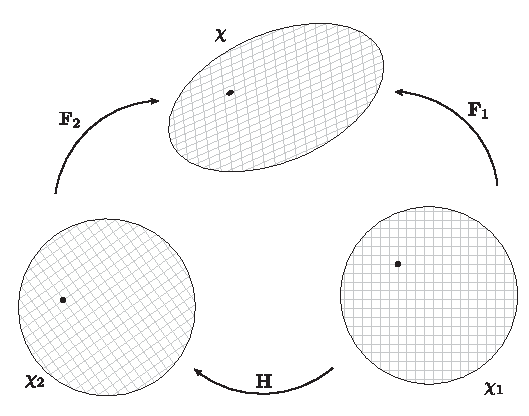
\includegraphics[width=0.7\linewidth]{figure/assunzioni_costitutive/materialSymmetry}
	\caption{A sketch of the regions occupied by a body in a (current) configuration $\chi$ and two reference
		configurations $\chi_1$ and $\chi_2$. The deformation gradient tensors from $\chi_1\to\chi$ and $\chi_2\to\chi$ are $\Fb_1$ and $\Fb_2$.
		The stress at a point  in the deformed configuration is $\Tb$ and is independent of the choice of reference
		configuration.}
	\label{fig:materialsymmetry}
\end{figure}
 
Let \( \widehat{\mathbf{T}}_1 \) and \( \widehat{\mathbf{T}}_2 \) be the stress response functions associated with these two reference configurations.  
Since the Cauchy stress in the current configuration is given both by  
\[
\mathbf{T} = \widehat{\mathbf{T}}_1(\mathbf{F}_1) \quad \text{and} \quad \mathbf{T} = \widehat{\mathbf{T}}_2(\mathbf{F}_2),
\]  
we must have  
\[
\widehat{\mathbf{T}}_2(\mathbf{F}_2) = \widehat{\mathbf{T}}_1(\mathbf{F}_1).
\]

Let \( \mathbf{H} \) be the gradient of the mapping (at \( \xb \)) from the first reference configuration to the second.  
Then \( \mathbf{F}_1 = \mathbf{F}_2 \mathbf{H} \), and so we must have  
\[
\widehat{\mathbf{T}}_2(\mathbf{F}) = \widehat{\mathbf{T}}_1(\mathbf{F} \mathbf{H}) \quad \text{for all nonsingular } \mathbf{F}.
\]  
Thus, if we know the stress response function \( \widehat{\mathbf{T}}_1 \) associated with one reference configuration,  
and the mapping \( \mathbf{H} \) from it to another reference configuration,  
the stress response function in the second reference configuration can be determined from the preceding equation.  

If the two reference configurations happen to be such that  
\[
\widehat{\mathbf{T}}_1(\mathbf{F}) = \widehat{\mathbf{T}}_2(\mathbf{F}) \quad \text{for all nonsingular } \mathbf{F},
\]  
then these two reference configurations have the same stress response functions; see Figure~\ref{fig:materialsymmetry1}. 

\begin{figure}
	\centering
	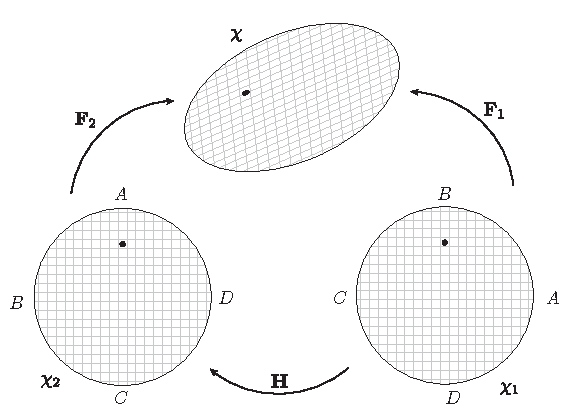
\includegraphics[width=0.7\linewidth]{figure/assunzioni_costitutive/materialSymmetry1}
	\caption{A sketch of the regions occupied by a body in a (deformed) configuration \( \chi \) and two reference configurations \( \chi_1 \) and \( \chi_2 \). The locations of four material points \( A, B, C, D \) in the two reference configurations are shown. Note the symmetry between the reference configurations \( \chi_1 \) and \( \chi_2 \), even though they are distinct. The transformation \( \Hb \) from \( \chi_1 \rightarrow \chi_2 \) preserves the symmetry of the material.}
	\label{fig:materialsymmetry1}
\end{figure}
 
Consider the set of all tensors \( \mathbf{H} \) that take \( \chi_1 \) to a configuration with the identical stress response function.  
This set is  
\[
\left\{ \mathbf{H} : \det \mathbf{H} \neq 0,\ \widehat{\mathbf{T}}(\mathbf{F}) = \widehat{\mathbf{T}}(\mathbf{F} \mathbf{H})\ \text{for all nonsingular } \mathbf{F} \right\}.
\]


This is the set of transformations of the reference configuration that leave the stress response  
function unchanged.  

Next, recall that the mass densities \( \rho_1 \) and \( \rho_2 \) in the two reference configurations are  
related by  
\[
\rho_2 = \rho_1 |\det \mathbf{H}|.
\]  
The mass densities in the two reference configurations are identical if \( |\det \mathbf{H}| = 1 \).  

We say that two configurations are \emph{mechanically indistinguishable} from each other  
if their mass densities and stress response functions coincide.  
Thus, in order to study mechanically indistinguishable configurations,  
we must restrict attention to tensors \( \mathbf{H} \) whose determinant is \( \pm 1 \).  
(If \( \det \mathbf{H} = -1 \), such a tensor could not be the deformation gradient of  
an actual deformation, since \( \det \mathbf{H} > 0 \) is required.  
However, we admit such tensors in our discussion of symmetry,  
as we wish to include reflection tensors among the set of permissible symmetry transformations.)  

A tensor with determinant equal to \( \pm 1 \) is said to be \emph{unimodular}.
The set of all tensors with \(\det\mathbf{H} = \pm 1\) forms the \emph{unimodular group}
\[
\Uc \;=\; \bigl\{\mathbf{H} : \det\mathbf{H} = \pm 1\bigr\}.
\]

In view of the two preceding observations we consider the set of tensors  
\begin{definition}

\begin{equation}\label{symgr}
	\Gc \;=\; \bigl\{\mathbf{H} \in \Uc,\;
\widehat{\mathbf{T}}(\mathbf{F}) = \widehat{\mathbf{T}}(\mathbf{F}\mathbf{H})
\;\text{for all nonsingular } \mathbf{F}\bigr\}.
\end{equation}

\end{definition}

The set \(\Gc\) characterizes all configurations that are mechanically indistinguishable from
\(\chi_1\); it is called the \emph{material symmetry group} of the configuration \(\chi_1\).

Symmetry is a property of a configuration: in general, the same body may possess
different symmetries in different configurations.  
Symmetry transformations are precisely those that leave the “material micro\-structure”
invariant.

From~\eqref{symgr} one can show that  
\begin{enumerate}
	\item  if \(\mathbf{H}_1 \in \Gc\) and \(\mathbf{H}_2 \in \Gc\) then \(\mathbf{H}_1\mathbf{H}_2 \in \Gc\); and  
\item  if \(\mathbf{H} \in \Gc\) then \(\mathbf{H}^{-1} \in \Gc\). 
\end{enumerate} 
Therefore \(\Gc\) is a group.\footnote{That is, \(\Gc\) is closed under multiplication and inversion.}

\medskip
We could equally well base the symmetry discussion on the free-energy potential
\(\widehat{\psi}(\mathbf{F})\), in which case  
\[
\Gc \;=\; \bigl\{\mathbf{H} : \det\mathbf{H} = \pm 1,\;
\widehat{\psi}(\mathbf{F}) = \widehat{\psi}(\mathbf{F}\mathbf{H})
\;\text{for all nonsingular } \mathbf{F}\bigr\}
\]
would describe the symmetry of a configuration.  
%(The reader may verify the relation between the two definitions, recalling that
\(\widehat{\mathbf{T}}(\mathbf{F}) = \rho_0 J^{-1}\,\widehat{\psi}_{\mathbf{F}}(\mathbf{F})\,\mathbf{F}^\top\).)

\medskip

From \eqref{symgr}  it follows that the material symmetry group is a subset of the unimodular group,
\[
\Gc \;\subset\; \Uc. 
\]

In principle, \(\Gc\) may coincide with any subgroup of \(\Uc\).
Two notable subgroups are the set of orthogonal tensors Orth and the set of all rotations about a fixed axis.
Frequently, \(\Gc\) consists of selected rotations and/or reflections.

Using material symmetry together with frame indifference,
one can show that 
\begin{definition}

\begin{equation}\label{matsym}
\Qb\in\Gc \qquad \Longleftrightarrow\qquad	\widehat{\mathbf{T}}\bigl(\mathbf{Q}\mathbf{F}\mathbf{Q}^\top\bigr)
\;=\;
\mathbf{Q}\,\widehat{\mathbf{T}}(\mathbf{F})\,\mathbf{Q}^\top
\quad\text{for all nonsingular } \mathbf{F}, 
\end{equation}

\end{definition}
or, equivalently, in terms of the free energy,
\[
\widehat{\psi}\bigl(\mathbf{Q}\mathbf{F}\mathbf{Q}^\top\bigr)
\;=\;
\widehat{\psi}(\mathbf{F})
\quad\text{for all nonsingular } \mathbf{F}.
\]

In order to prove \eqref{matsym}, we  will proceed in steps.
\begin{enumerate}
	\item ($\Rightarrow$) Assume $\mathbf{Q} \in \mathcal{G}$ and that the frame indifference holds:
	\begin{equation}\label{FI1}
		\widehat{\Tb}(\Qb\Fb)=\Qb\widehat{\Tb}(\Fb)\Qb^\top.
	\end{equation}
Let us define $\Gb=\Fb\Qb^\top$, so that $\Qb\Gb=\Qb\Fb\Qb^\top$. From the frame indifference \eqref{FI1}, we get
\begin{equation}\label{FI2}
	\widehat{\Tb}(\Qb\Gb)=\Qb\widehat{\Tb}(\Gb)\Qb^\top;
\end{equation}
since $\Qb\in\Gc$ by hypothesis,
\begin{equation}
	\widehat{\Tb}(\Gb)=	\widehat{\Tb}(\Gb\Qb)=\widehat{\Tb}(\Fb).
\end{equation}
Therefore \eqref{FI2}  and the definition of $\Gb$ imply
\begin{equation}\label{mats}
		\widehat{\Tb}(\Qb\Fb\Qb^\top)=\Qb\widehat{\Tb}(\Fb)\Qb^\top.
\end{equation}
We have then proved  that $\Qb\in\Gc$ implies \eqref{mats}.
\item ($\Leftarrow$) Assume $	\widehat{\Tb}(\Qb\Fb\Qb^\top)=\Qb\widehat{\Tb}(\Fb)\Qb^\top$ and that the the frame indifference \eqref{FI1} holds . Let now $\Gb=\Fb\Qb$, so that $\Fb=\Gb\Qb^\top$. Because of the hypothesis,
\begin{equation}
	\widehat{\Tb}(\Qb\Gb\Qb^\top)=\Qb\widehat{\Tb}(\Gb)\Qb^\top \qquad \Longrightarrow\qquad 	\widehat{\Tb}(\Qb\Fb)=\Qb\widehat{\Tb}(\Fb\Qb)\Qb^\top.
\end{equation}
By the frame indifference \eqref{FI1} applied to the lhs,  this is equivalent to 
\begin{equation}
\Qb\widehat{\Tb}(\Fb)\Qb^\top=\Qb\widehat{\Tb}(\Fb\Qb)\Qb^\top, 
\end{equation}
or equivalently,
\begin{equation}
\widehat{\Tb}(\Fb)=\widehat{\Tb}(\Fb\Qb).
\end{equation}
We therefore conclude that $\Qb\in\Gc$.
\end{enumerate}

\begin{remark}
	As noted earlier, symmetry is fundamentally a property of a particular configuration of a body. However, when the context is clear and there is no risk of misunderstanding, we will adopt the common (though imprecise) practice of attributing symmetry to the material itself. For example, we will refer to an ``isotropic material'' to mean that the material is considered in a configuration where it exhibits isotropy, and similarly for other symmetry types.
\end{remark}

\subsection{ Examples of Material Symmetry Groups}
\begin{enumerate}
	\item The largest possible material symmetry group is the unimodular group itself:
	\[
	\mathcal{G} = \mathcal{U}.
	\]
	If the material symmetry group of a certain configuration of a body is the unimodular group, one can show that
	\[
	\widehat{\mathbf{T}}(\mathbf{F}) = f(\det \mathbf{F}) \, \mathbf{I},
	\]
	i.e., the Cauchy stress is hydrostatic and depends on the deformation only through the Jacobian $\det \mathbf{F}$. Thus, the body responds as a fluid. If the material symmetry group in one configuration is $\mathcal{U}$, then it is $\mathcal{U}$ in every configuration. Therefore, if the body behaves as a fluid in one configuration, it behaves as a fluid in all configurations.
\item Let $\mathbf{R}^\varphi_\eb$ denote the rotation through an angle $\varphi$ about an axis $\eb$. The set of all such rotations about a fixed axis $\eb$,
\[
\left\{ \mathbf{R}^\varphi_\eb \mid 0 \leq \varphi \leq 2\pi \right\},
\]
forms a group. If the material symmetry group coincides with this group, we say that the body is \textit{transversely isotropic} about the axis $\eb$ in this reference configuration.
\item If the material symmetry group is generated by $\pi/2$ rotations $\mathbf{R}^{\pi/2}_{\eb_1}$, $\mathbf{R}^{\pi/2}_{\eb_2}$, and $\mathbf{R}^{\pi/2}_{\eb_3}$ about the three orthonormal vectors $\{ \mathbf{e}_1, \mathbf{e}_2, \mathbf{e}_r \}$, then the material is said to be \textit{cubic} in this reference configuration.
\item If $\Gc=$Orth, we say that the body is \textit{isotropic} in this reference configuration.
\end{enumerate}


\section{Isotropic materials}
Up to this point, we have focused on how to characterize a material's symmetry. We now turn to understanding how this symmetry can be used to further simplify the constitutive relations.
Let us consider an isotropic material. In this case $\widehat{\psi}(\Qb\Fb\Qb^\top)=\widehat{\psi}(\Fb)$ for all $\Qb\in$Orth. In this event, one can show that $\widehat{\psi}$ has the representation
\begin{equation}
\widehat{\psi}(\Fb)=\psi (I_1(\Cb), I_2(\Cb), I_3(\Cb)),
\end{equation}
where 
\begin{equation}
	I_1(\Cb) = \text{tr}\, \Cb, \quad I_2(\Cb) = \frac{1}{2} \left[(\text{tr}\, \Cb)^2 - \text{tr}(\Cb^2)\right], \quad I_3(\Cb) = \det \Cb = (\det\Fb)^2=J^2, 
\end{equation}
are the principal scalar invariants of the right Cauchy-Green tensor $\Cb = \Fb^\top \Fb = \Ub^2$. (Recall that the eigenvalues and principal scalar invariants of $\Cb$ and $\Bb = \Fb \Fb^\top = \Vb^2$ coincide.) On differentiating with respect to $\Cb$ we find
\begin{equation}\label{derinv}
	\frac{\partial I_1}{\partial \Cb} = \Ib, \quad \frac{\partial I_2}{\partial \Cb} = I_1 \Ib - \Cb, \quad \frac{\partial I_3}{\partial \Cb} = J^2 \Cb^{-1}.
\end{equation}

In order to determine the stress tensor $\Pb$, we may use \eqref{constP} $\Pb = 2\rho_0 \Fb \partial_\Cb\widehat{\psi}$; and since $\Tb = J^{-1} \Pb \Fb^\top$, it follows that
\begin{definition}
	\[
\Tb = 2\rho_0 J^{-1} \Fb \partial_\Cb\widehat{\psi}\Fb^\top,
\]
\end{definition}
which can be used to find $\Tb$. Using these, together with the chain rule and \eqref{derinv}, lead to the following constitutive relations for an elastic material with respect to an isotropic reference configuration:
\begin{equation}
	\left.
	\begin{aligned}
		\rho_0^{-1} \Tb &= 2J \frac{\partial \psi}{\partial I_3} \Ib + \frac{2}{J} \left( \frac{\partial \psi}{\partial I_1} + I_1 \frac{\partial \psi}{\partial I_2} \right) \Bb - \frac{2}{J} \frac{\partial \psi}{\partial I_2} \Bb^2, \\
		\rho_0^{-1} \Pb &= 2 I_3 \frac{\partial \psi}{\partial I_3} \Fb^{-T} + 2 \left( \frac{\partial \psi}{\partial I_1} + I_1 \frac{\partial \psi}{\partial I_2} \right) \Fb - 2 \frac{\partial \psi}{\partial I_2} \Bb \Fb.
	\end{aligned}
	\right\} 
\end{equation}
Note that for an isotropic material, the principal directions of $\Tb$ and $\Bb$ coincide.


\section{Materials with Internal Constraints}
%Abeyaratne
Thus far, we have assumed that the body under consideration can undergo any motion at all by subjecting it to suitable body forces and surface tractions. In certain circumstances, it is possible, and indeed convenient, to idealize the body such that it can only undergo motions of a certain restricted class. 

For example, a \textit{rigid} body can only undergo rigid motions, i.e., motions in which $\Fb(\mathbf{\xb}, t)$ is independent of $\mathbf{x}$ and is proper orthogonal at all $t$; an \textit{incompressible} body can only undergo volume-preserving motions, i.e., motions in which $\det \Fb(\mathbf{\xb}, t) = 1$; a body which is inextensible in a certain (referential) direction $\mathbf{\eb}$ can only undergo motions in which $|\Fb(\mathbf{x}, t)\mathbf{e}| = 1$ at every particle and instant.

A material is said to be subjected to a \textit{simple internal constraint} if it can only undergo motions in which
\begin{equation}\label{constr}
	\widehat\phi(\Fb(\mathbf{x}, t)) = 0 \quad \text{for all } \mathbf{x} \in \widetilde\Omega, \, t \in [t_0, t_1],
\end{equation}
where the function $\widehat\phi$ describes the constraint. The constraints of rigidity, incompressibility, and inextensibility are described by
\[
\widehat\phi(\Fb) = \Fb^\top \Fb - \Ib, \quad \widehat\phi(\Fb) = \det \Fb - 1, \quad \text{and} \quad \widehat\phi(\Fb) = \Fb\mathbf{\eb} \cdot \Fb\mathbf{\eb} - 1,
\]
respectively.

It is natural to require the constraint \eqref{constr} to be material frame indifferent, i.e., if a deformation gradient tensor $\Fb$ obeys the constraint  \eqref{constr}, a subsequent rigid rotation should not lead to a violation of the constraint. That is, if $\Fb$ obeys  \eqref{constr}, then $\Qb\Fb$ must also satisfy  \eqref{constr} for every rotation $\Qb$. Accordingly, we require that
\[
\widehat\phi(\Fb) = \widehat\phi(\Qb\Fb) \quad \text{for all nonsingular tensors } \Fb \text{ and all rotations } \Qb.
\]
The discussion on objectivity can be readily adapted to the present context to show that  \eqref{constr} is objective if and only if the constraint can be expressed in the form
\begin{equation}
	\phi(\Cb(\mathbf{\xb}, t)) = 0 \quad \text{for all } \mathbf{x} \in \widetilde{\Omega}, \, t \in [t_0, t_1], \tag{8.48}
\end{equation}
where $\Cb = \Fb^\top \Fb$. Observe that the three examples given earlier can be expressed in this form: rigidity as $\Cb = \Ib$, incompressibility as $\det \Cb = 1$, and inextensibility as $\Cb\mathbf{e} \cdot \mathbf{e} = 1$.

We now consider the stresses in a constrained body. In order to explain the basic idea, consider as an example, a sphere composed of an incompressible isotropic material that is subjected to a uniform applied pressure $\pi$ on its boundary. Since the geometry, the material, and the loading are all symmetric, let us restrict attention to spherically symmetric deformations. Thus, the sphere can only become a smaller/larger sphere when $\pi$ is applied. However, due to incompressibility, the sphere cannot remain spherical and change its size.

Thus, irrespective of the value of $\pi$, incompressibility implies that any symmetric deformation of the sphere must be the trivial one: $\widehat{\yb}(\mathbf{x}, t) = \mathbf{x}$ and therefore necessarily $\Fb(\mathbf{x}, t) = \Ib$ no matter what the value of $\pi$. The stress, on the other hand, would certainly depend on the value of the applied pressure $\pi$. Thus, the stress $\Tb$ is not completely determined by the deformation gradient $\Fb$, or equivalently,\textit{ different stress fields can correspond to the same deformation}. 

This contradicts our earlier notion of determinism, according to which the stress is completely determined by the history of the motion until time $t$. We must therefore modify this notion when considering a constrained body.

It is customary to suppose that the stress $\Tb^{(\rm A)}$ can be additively decomposed into two parts: one that is determined by the history of the deformation gradient tensor $\Fb$, and the other, say $\Tb^{(\rm R)}$, that is not. The stress $\Tb^{(\rm R)}$ is assumed to spend no power in any motion consistent with the constraint. Thus, for example, one might have
	\begin{equation}\label{Tar}
	\Tb = \widetilde{\Tb}^{(\rm A)}(\Fb, \dot{\Fb}) + \Tb^{(\rm R)},
\end{equation}
where
\begin{equation}\label{recpow}
	 \Tb^{(\rm R)} \cdot \Db = 0 
\end{equation}
for all stretching tensors $\Db$ consistent with the constraint \eqref{constr}. The stress field $\Tb^{(\rm R)}$ arises in ``\textit{reaction}'' to the constraint and is often referred to as the \textit{reaction stress}. One sometimes refers to $ \widetilde{\Tb}^{(\rm A)}$ and $ \Tb^{(\rm R)}$ as the \textit{active} and \textit{reactive} parts of the stress.

Note that \eqref{recpow} does not hold for all symmetric $\Db$ but only for those that are consistent with the constraint  \eqref{constr}. Thus, we now determine the restriction that the constraint places on the stretching tensor. Differentiating \eqref{constr} with respect to $t$ shows that
\begin{equation}
	\partial_\Cb\phi(\Cb) \cdot \dot{\Cb} = 0. 
\end{equation}
On making use of the kinematic identity $\dot{\Cb} = 2 \Fb^\top \Db \Fb$, we get the following restriction on the possible values of $\Db$:
\begin{equation}\label{ort}
	\Fb \, 	\partial_\Cb\phi(\Cb) \, \Fb^\top \cdot \Db = 0.
\end{equation}
This equation states that $\Db$ is orthogonal to $\Fb \partial_\Cb\phi(\Cb) \Fb^\top$. Equations \eqref{recpow} and \eqref{ort} together state that the tensor $ \Tb^{(\rm R)} $ is orthogonal to every tensor $\Db$ that is orthogonal to $\Fb \partial_\Cb\phi(\Cb)\Fb^\top$. Thus, $\Tb^{(\rm R)} $ must be parallel to $\Fb\partial_\Cb (\Cb) \Fb^\top$, and so there exists a scalar field $\lambda(\mathbf{x}, t)$ such that
\begin{definition}
\begin{equation}\label{reac}
	\Tb^{(\rm R)}  = \lambda \, \Fb \, \partial_\Cb\phi(\Cb) \, \Fb^\top.
\end{equation}
\end{definition}

\vspace{.3cm}

As an example, consider an incompressible body, in which case $\phi(\Cb) = \det \Cb - 1$. Thus,
\[
\partial_\Cb\phi(\Cb) = (\det \Cb) \Cb^{-\top} = \Cb^{-1},
\]
so that \eqref{reac} yields the well-known result
\begin{equation}
	\Tb^{(\rm R)}	 = \lambda \Ib 
\end{equation}
which says that the reaction stress is a pressure.

Similarly, for a body that is inextensible in the referential direction $\mathbf{e}$, one finds that
\begin{equation}
		\Tb^{(\rm R)}= \lambda \, \Fb\mathbf{e} \otimes \Fb\mathbf{e};
\end{equation}
here $	\Tb^{(\rm R)}$ is a uniaxial stress in the fiber direction $\mathbf{e}$.



%
%\newpage
%A material is elastic if
%\begin{enumerate}
%	\item The energy $\psi$ and the stress $\Tb$ depend only on the current value of the deformation and not on its past history or the rate at which the deformation changes. As a consequence, the constitutive equations for energy and stress are of the form
%	\begin{equation}\label{constel}
%	%	\psi = \widehat{\psi}(\Fb), \qquad \Tb = \widehat{\Tb}(\Fb).
%		\psi_{\rm ref}=\widehat{\psi}_{\rm ref}(\Fb), \qquad \Pb=\widehat{\Pb}(\Fb).
%	\end{equation}
%	\item It does not dissipate energy:
%	\begin{equation}
%		\rho\gamma = \Tb \cdot \Db - \rho\dot{\psi} = 0.
%	\end{equation}
%\end{enumerate}
%
%\section{Consequences of frame-indifference}
%%For an elastic body we can give  the free energy and stress when $\Fb$ is known:
%%\begin{equation}\label{consteq}
%%	\begin{aligned}
%%		\psi_{\rm ref}=\widehat{\psi}_{\rm ref}(\Fb), \qquad \Pb=\widehat{\Pb}(\Fb).
%%	\end{aligned}
%%\end{equation}
%Because we have in mind to focus on solids, it is more convenient to work in the referential setting; this is emphasized by the subscript `ref' in those fields that may have referential and current counterparts. 
%
%The response functions $\widehat{\psi}_{\rm ref}$ and $\widehat{\Pb}$ can be use to determine the constitute equations for the Cauchy and second Piola stress:
%\begin{equation}\label{C2Pce}
%	\Tb=\widehat{\Tb}(\Fb)=(\det\Fb)^{-1}\widehat{\Pb}(\Fb)\Fb^\top, \qquad \Sb=\widehat{\Sb}(\Fb)=\Fb^{-1}\widehat{\Pb}(\Fb).
%\end{equation}
%
%We now explore the consequences of the hypotheses  stipulating that
%the constitutive equations be frame-indifferent and compatible with thermodynamics.
%
%Since the deformation gradient transforms according to $\Fb^+=\Qb\Fb$,
%\begin{eqnarray}
%	\widehat{\psi}_{\rm ref}(\Fb)=\widehat{\psi}_{\rm ref}(\Qb\Fb).
%\end{eqnarray}
%From \eqref{Pio} it is easy to see that $\Pb^+=\Qb\Pb$, so that
%\begin{equation}
%	\Pb^+=\widehat{\Pb}(\Fb^+)=\widehat{\Pb}(\Qb\Fb).
%\end{equation}
%
%The response maps $\widehat{\psi}_{\rm ref}$ and $\widehat{\Pb}$ must therefore satisfy
%\begin{equation}
%	\widehat{\psi}_{\rm ref}(\Fb)=\widehat{\psi}_{\rm ref}(\Qb\Fb), \quad \widehat{\Pb}(\Fb)=\Qb^\top\widehat{\Pb}(\Qb\Fb),
%\end{equation}
%for all rotations $\Qb$ and $\Fb$. Fix $\Fb$ and consider the polar decomposition $\Fb=\Rb\Ub$. Since $\Qb$ is arbitrary, we choose $\Qb=\Rb^\top$; hence $\Qb\Fb=\Ub$ and
%\begin{equation}
%	\widehat{\psi}_{\rm ref}(\Fb)=\widehat\psi_{\rm ref}(\Ub), \quad \widehat{\Pb}(\Fb)=\Rb\widehat{\Pb}(\Ub).
%\end{equation}
%Replacing $\Ub$ by $\sqrt{\Cb}$, we may introduce a response function $\widetilde{\psi}_{\rm ref}$ determining the free energy $\psi_{\rm ref}$ as a function of $\Cb$ via
%\begin{equation}
%	\widetilde{\psi}_{\rm ref}(\Cb)=\widehat\psi_{\rm ref}(\sqrt{\Cb}).
%\end{equation}
%Similarly, in view of \eqref{C2Pce}$_2$ for the second Piola stress we find that
%\begin{equation}
%	\Rb\widehat{\Pb}(\Ub)=\Fb\Ub^{-1}\widehat{\Pb}(\Ub)=\Fb\widehat{\Sb}(\Fb)=\Rb\Ub\widehat{\Sb}(\Fb).
%\end{equation} 
%Hence  $\widehat{\Pb}(\Ub)=\Ub\widehat{\Sb}(\Fb)$,
%\begin{equation}
%	\widehat{\Sb}(\Fb)=\Ub^{-1}\widehat{\Pb}(\Ub),
%\end{equation}
%and, replacing $\Ub$ by $\sqrt{\Cb}$, we may introduce a response function $\widetilde{\Sb}$ determining the second Piola stress as a function of $\Cb$:
%\begin{equation}
%	\Sb=\Cb^{-1/2}\widehat{\Pb}(\sqrt{\Cb})=\widetilde{\Sb}(\Cb).
%\end{equation}
%
%If the constitutive equations \eqref{constel} are to be frame-indifferent, the foregoing results show that they must reduce to constitutive equations of the specific form
%\begin{equation}
%	\psi_{\rm ref}=\widetilde{\psi}_{\rm ref}(\Cb), \qquad \Pb=\Fb\widetilde{\Sb}(\Cb).
%\end{equation}
%
%Since the second Piola stress is symmetric, an important consequence of this latter relation is that
%\begin{equation}
%	\Pb\Fb^\top-\Fb\Pb^\top=\Fb\Sb\Fb^\top-\Fb\Sb^\top\Fb^\top=\Fb(\Sb-\Sb^\top)\Fb^\top=\mathbf{0}.
%\end{equation}
%Hence the requirement that the constitutive equations be frame-indifferent implies satisfaction of the moment balance. Granted frame-indifferent constitutive equations, we may therefore neglect the moment balance from further consideration.


\section{Infinitesimal theory}
It is possible to write the constitutive equation for the stress in terms of the displacement $\ub(\xb)=\fb(\xb)-\xb$:
\begin{equation}
\Tb(\yb)=\widehat{\Tb}(\Ib +\Hb(\xb)).
\end{equation}
If $\widehat{\Tb}$ is sufficiently smooth, we may write
\begin{equation}
\Tb(\yb)=\widehat{\Tb}(\Ib)+\partial_\Fb \widehat{\Tb}(\Ib)\,\Hb+o(|\Hb|).
\end{equation}
The term $=\widehat{\Tb}(\Ib)$ represents the stress in the referential configuration, that we assume null. With this, and \eqref{C2Pce}$_1$, we have
\begin{equation}
\Pb(\xb)=\det \Fb(\xb)\, \Tb(\yb) \Fb^{-\top}(\xb)=\det \Fb(\xb)\, \big( \partial_\Fb \widehat{\Tb}(\Ib)\,\Hb+o(|\Hb|) \big) \Fb^{-\top}(\xb).
\end{equation}
If we argument as in chapter \ref{inf}, we deduce that
\begin{equation}
\Pb=(1+\operatorname{tr}\Hb)\,  \big( \partial_\Fb \widehat{\Tb}(\Ib)\,\Hb+o(|\Hb|) \big) (\Ib-\Hb^{-\top})=\partial_\Fb \widehat{\Tb}(\Ib)\,\Hb+o(|\Hb|),
\end{equation}
and then
\begin{definition}
\begin{equation}
\Pb(\xb)=\Tb(\yb)+o(|\Hb|).
\end{equation}
\end{definition}
Therefore, up to infinitesimals of order \( o(|\Hb|) \), the Cauchy stress tensor evaluated at \( \fb(\xb) \) is equal to the Piola stress tensor evaluated at \( \xb \):
Identifying the configuration determined by the deformation \( \fb \) with the reference configuration introduces an error of order \( o(|\Hb|) \). More precisely, up to infinitesimals of order \( o(|\Hb|) \), it is possible to define a stress tensor---still referred to as the Cauchy stress tensor and denoted by \( \Tb \)---on the reference configuration such that:
\begin{enumerate}
	\item  \( \Tb(\xb) = \Tb(\xb) \) for every \( \xb \in \Omega = \kappa(\Bb) \);
	\item  the equilibrium equation  becomes  
	\[
	\operatorname{Div}\Tb(\xb) + \bb(\xb) =\mathbf{0}
	\]  
	for every \( \xb \in \Omega \), where \( \bb \) denotes the body forces per unit volume in the reference configuration;
\item  \( \Tb(\xb)\nb(\xb) \) represents the stress at the point \( \fb(\xb) \) along a surface whose preimage has normal \( \nb \).
\end{enumerate}

For sake of simplicity, \textit{in the following we will just consider the infinitesimal theory}. Therefore, 
 we can write the following constitutive equations:
\begin{equation}
\Tb=\widehat{\Tb}(\Eb), \qquad \psi=\widehat{\psi}(\Eb).
\end{equation}
 Moreover, we set
\begin{equation}
\rho\varepsilon=\bar{\varepsilon}, \quad \rho\eta=\bar{\eta}, \quad \rho\delta=\bar\delta, \quad \rho \psi=\bar{\psi}.
\end{equation}
We will work with the barred quantities, but omit the bars in the notation. Eventually, no difference will be between $\nabla\varphi$, $\grad\varphi$, $\Div\varphi$ and $\dive\varphi$.


\section{Consequences of thermodynamic restrictions}
To understand the consequences of the thermodynamic restrictions, we use the Coleman-Noll procedure. 

Since the process is given by $\psi = \widehat{\psi}(\Eb)$ and $\Tb = \widehat{\Tb}(\Eb)$, equation \eqref{gammael} can be rewritten as
\begin{equation}
	\widehat{\Tb}(\Eb) \cdot \dot{\Eb} - \left(\widehat{\psi}(\Eb)\right)^{\mathop{\vcenter{\hbox{\Large$\cdot$}}}} = 0,
\end{equation}
or, using the chain rule
\begin{equation}\label{Tepsi}
	\left( 	\widehat{\Tb}(\Eb) - \partial_\Eb \widehat{\psi} \right) \cdot \dot{\Eb} = 0.
\end{equation}

This condition must be satisfied for every local continuation of any conceivable process; in particular, we assume that the geometry of the state space is such that a local continuation of any trajectory in the space is accessible.

In other words, for every pair $(\Sc, \dot{\Sc})$, we assume that there exists a trajectory $t \mapsto \Sc(t)$ and an instant of time $t_0$ such that $\Sc(t_0) = \Sc$ and $\dot{\Sc}(t_0) = \dot{\Sc}$.

In this context, this means that equation \eqref{Tepsi} must hold \textit{for every} $\dot{\Eb}$ and therefore
\begin{definition}
	\begin{equation}\label{Tdevpsi}
		\widehat{\Tb}(\Eb) = \partial_\Eb \widehat{\psi}(\Eb).
	\end{equation}
\end{definition}
Such a material is called \textit{hyperelastic}.

For \textit{linear elastic materials}, we consider an expansion of the constitutive response function of stress around a \textit{relaxed} reference configuration, that is, with $\Eb = \mathbf{0}$, $\psi = 0$, and $\Tb = \mathbf{0}$; the requirement that $\Tb$ is zero in the reference configuration is not fundamental and can be removed, leading to materials with self-stresses or residual stresses. Thus, we have
\begin{equation}
	\widehat{\Tb} = \widehat{\Tb}(\mathbf{0}) + \left(\left.\partial_\Eb \widehat{\Tb}(\Eb)\right|_{\Eb = \mathbf{0}}\right)\,\Eb + o(|\mathbf{E}|).
\end{equation}
Since the reference configuration is relaxed, $\widehat{\Tb}(\mathbf{0}) = \mathbf{0}$. Due to equation \eqref{Tdevpsi}, we can write
\begin{equation}
	\left.\partial_\Eb \widehat{\Tb}(\Eb)\right|_{\Eb = \mathbf{0}} = \left.\partial^2_{\Eb \Eb} \widehat{\psi}(\Eb)\right|_{\Eb = \mathbf{0}} =: \Co,
\end{equation}
where we have introduced the elasticity tensor (of fourth order) $\Co$. Neglecting infinitesimals of order $o(|\Eb|)$, we can then write the constitutive response map for stress:
\begin{definition}
	\begin{equation}
		\Tb = \widehat{\Tb}(\Eb) = \Co \Eb, \qquad \qquad (T_{ij} = \Co_{ijhk} E_{kh})
	\end{equation}
\end{definition}
The associated energy, due to equation \eqref{Tdevpsi}, is given by the following constitutive response map:
\begin{definition}
	\begin{equation}
		\psi = \widehat{\psi}(\Eb) = \frac{1}{2} \Co \Eb \cdot \Eb, \qquad \qquad \left(\psi = \frac{1}{2} \Co_{ijhk} E_{ij} E_{hk} \right)
	\end{equation}
\end{definition}

Since
\begin{equation}
	\frac{\partial^2 \widehat{\psi}(\Eb)}{\partial E_{ij} \partial E_{hk}} = \frac{\partial^2 \widehat{\psi}(\Eb)}{\partial E_{hk} \partial E_{ij}},
\end{equation}
it follows that the components $\Co_{ijhk}$ of $\Co$ possess the so-called \textit{major symmetries}:
\begin{definition}
	\begin{equation}
		\Co_{ijhk} = \Co_{hkij}.
	\end{equation}
\end{definition}

Furthermore, since $\Tb \in \Sym$,
\begin{equation}
	T_{ij} = \Co_{ijhk} E_{hk} = T_{ji} = \Co_{jihk} E_{hk},
\end{equation}
the components $\Co_{ijhk}$ of $\Co$ also possess the so-called \textit{minor symmetries}:

\begin{definition}
	\begin{equation}
		\Co_{ijhk} = \Co_{jihk}.
	\end{equation}
\end{definition}

For the minor symmetries, the components of $\Co$ are at most $6^2 = 36$; indeed, considering $\Co_{ijhk}$, the pair $ij$, due to symmetry, produces at most 6 independent components, and the same holds for the pair $hk$.

The major symmetry further reduces the number of components to at most $36 - 15 = 21$.


\section{Material symmetries}
We say that $\Qb$ represents a material symmetry if rotations or reflections of the material by $\Qb$ cannot be detected through stress-strain experiments.

Suppose we have a material made of a matrix in which fibers are embedded in the direction $\eb_1$. Imagine measuring the stress required to produce an extension $\varepsilon$ in the $\eb_1$ direction, that is, by imposing the strain
\begin{equation}
	\Eb =\varepsilon\,\eb_1\otimes\eb_1.
\end{equation}
Now imagine measuring the stress required to produce an extension equal to $\varepsilon$ but in a direction rotated by $\Qb=\Rb (\pi/2, \eb_3)$, that is, by $\pi/2$ about $\eb_3$:
\begin{equation}
	\Eb ^\Qb =\varepsilon\, \eb_2 \otimes \eb_2= \varepsilon\,\Qb \eb_1 \otimes \Qb \eb_1.
\end{equation}

Clearly, we expect the stress measured in the second experiment to be different from the first one, and thus $\Qb$ does \textit{not} represent a material symmetry. A rotation by $\pi$, on the other hand, would not be detectable, since the material would be indistinguishable from the original one when rotated by $\pi$; in this case, $\Rb(\pi, \eb_3)$ would represent a material symmetry.

Let us now clarify what we mean by measuring the same stress in two different experiments, like those just described.

In a uniaxial test, a strain $\Eb=\varepsilon\,\eb_1\otimes\eb_1$ corresponds to a stress
\begin{equation}
	\Tb =\sigma \eb_1\otimes\eb_1.
\end{equation}
Now suppose we carry out the same experiment in a direction rotated by $\Qb=\Rb (\pi/2, \eb_3)$, applying an extension $\varepsilon$ in the $\eb_2$ direction, i.e., $\Eb^\Qb=\varepsilon\eb_2\otimes\eb_2$, and we measure the resulting stress:
\begin{equation}
	\Tb^\Qb =\sigma^\Qb\eb_2\otimes \eb_2.
\end{equation}
Clearly, the stress is the same if
\begin{equation}
	\sigma=\sigma^\Qb
\end{equation}
and not when $\Tb =\Tb ^\Qb$.

Let us generalize this through the example of uniaxial tension. By the spectral theorem, we can represent $\Eb$ as
\begin{equation}\label{espettr1}
	\Eb=\sum_{i=1}^{3}\varepsilon_i\, \vb_i\otimes \vb_i,
\end{equation}
where $(\varepsilon_i, \vb_i)$ are the eigenpairs of $\Eb$. The rotated strain $\Eb^\Qb$ is a strain with the same extensions $\varepsilon_i$ but in the directions rotated by $\Qb$:
\begin{equation}
	\Eb^\Qb\coloneqq \sum_{i=1}^{3}\varepsilon_i\, \Qb\vb_i\otimes \Qb\vb_i,
\end{equation}
that is,\footnote{Here we use the property valid for all $\Ab, \Bb\in$ Lin, $\ab, \bb \in \Vc$:
	\begin{equation}
		\Ab(\ab\otimes\bb)\Bb=\Ab \ab \otimes \Bb^\top \bb.
\end{equation}}
\begin{equation}
	\Eb^\Qb=\Qb\sum_{i=1}^{3}\varepsilon_i\, \vb_i\otimes \vb_i \Qb ^\top = \Qb \Eb \Qb^\top.
\end{equation}
Let us denote by 
\begin{equation}
	\Tb \coloneqq\Co \Eb, \qquad \Tb^\Qb\coloneqq \Co \Eb^\Qb=\Co (\Qb \Eb \Qb^\top)
\end{equation}
the responses to the strains $\Eb$ and $\Eb^\Qb$. Since $\Tb$ and $\Tb^\Qb$ are symmetric, we can write their spectral representation:
\begin{equation}
	\Tb=\sum_{i=1}^{3}\sigma_i\, \tb_i\otimes \tb_i, \qquad 	\Tb^\Qb=\sum_{i=1}^{3}\sigma_i\, \tb^\Qb_i\otimes \tb^\Qb_i.
\end{equation}
We will say that $\Qb\in$ Orth is a material symmetry if
\begin{equation}
	\sigma_i=\sigma_i^\Qb, \qquad \tb_i^\Qb=\Qb \tb_i,
\end{equation}
that is, if $\Eb$ and $\Eb^\Qb$ produce the same principal stresses in directions rotated by $\Qb$. 

Therefore, if $\Qb$ is a symmetry
\begin{equation}
	\Co(\Qb\Eb \Qb^\top)=\Co \Eb^\Qb=\Tb^\Qb=\sum_{i=1}^{3}\sigma_i\, \tb^\Qb\otimes \tb^\Qb=\Qb \left(  \sum_{i=1}^{3}\sigma_i\, \tb_i\otimes \tb_i \right)\Qb^\top=\Qb \Tb \Qb^\top=\Qb\Co \Eb \Qb^\top.
\end{equation}
We conclude that $\Qb\in$ Orth is a material symmetry if
\begin{definition}
	\begin{equation}
		\Co(\Qb\Eb \Qb^\top)=\Qb \Co \Eb \Qb ^\top \qquad \forall \Eb \in \Sym,
	\end{equation}
\end{definition}
that is,
\begin{definition}
	\begin{equation}
		\widehat{\Tb}(\Qb \Eb \Qb ^\top)=\Qb \widehat{\Tb}(\Eb)\Qb ^\top, \qquad \forall \Eb \in \Sym.
	\end{equation}
\end{definition}

The set
\begin{equation}
	\Gc =\{ \Qb \in {\rm Orth}\, :\, \widehat{\Tb}(\Qb \Eb \Qb ^\top)=\Qb \widehat{\Tb}(\Eb)\Qb ^\top, \quad \forall \Eb \in \Sym  \}
\end{equation}
is called the \textit{material symmetry group}, and its elements are the material symmetries.

\begin{exercise}
	Let $\mathcal{G}_{\mathbb{C}}$ be the symmetry group of an elastic material and $\psi=\widehat\psi(\Eb)$ the elastic energy density
	\begin{equation}
		\psi=\widehat\psi(\Eb)=\frac12 \Co\Eb\cdot\Eb.
	\end{equation}
	
	Show that, for every $\Qb\in\mathcal{G}_{\mathbb{C}}$,
	\begin{equation}
		\widehat\psi(\Eb)=	\widehat\psi(\Qb\Eb\Qb^\top).
	\end{equation}
	
	\begin{svolgimento}
		We have
		\begin{equation}
			\widehat{\psi}(\Eb)=\frac{1}{2}\widehat{\Tb}(\Eb)\cdot \Eb, \qquad \widehat{\psi}(\Qb\Eb\Qb^\top)=\frac{1}{2}\widehat{\Tb}(\Qb\Eb\Qb^\top)\cdot \Qb\Eb\Qb^\top.
		\end{equation}
		Since $\Qb \in \mathcal{G}_{\mathbb{C}}$
		\begin{equation}
			\widehat{\Tb}(\Qb\Eb\Qb^\top)=\Qb\widehat{\Tb}(\Eb)\Qb^\top,
		\end{equation}
		and thus
		\begin{equation}
			\widehat{\psi}(\Qb\Eb\Qb^\top)=\frac12\Qb\widehat{\Tb}(\Eb)\Qb^\top\cdot  \Qb\Eb\Qb^\top=\frac12 \Qb^\top\Qb \widehat{\Tb}(\Eb)\cdot \Eb \Qb^\top\Qb=\frac{1}{2}\widehat{\Tb}(\Eb)\cdot \Eb=\widehat{\psi}(\Eb).
		\end{equation}
		The result shows the obvious invariance of the energy with respect to material symmetry transformations.
	\end{svolgimento}
	
\end{exercise}


\section{Isotropic materials}
A material is isotropic if its elastic response is the same in all directions, namely
\begin{equation}
	\Gc ={\rm Orth},
\end{equation}
and therefore
\begin{equation}
	\widehat{\Tb}(\Qb \Eb \Qb ^\top)=\Qb \widehat{\Tb}(\Eb)\Qb ^\top, \qquad \forall \Eb \in \Sym, \Qb \in {\rm Orth}.
\end{equation}

A relevant property of an isotropic material, known as \textit{coaxiality}, is that
when it is subjected to deformation, the directions in which maximum and minimum strains occur (principal strain directions) are the same as those in which maximum and minimum stresses develop (principal stress directions). In other words, if one observes an isotropic material undergoing loading, the directions along which strains are maximum (e.g., stretching or compression) coincide with those along which stresses are maximum. This behavior reflects the uniformity of the material in all spatial directions. For example, if a material elongates along a principal direction, the stress causing this deformation will be oriented in the same direction.

We now state more precisely the 
\begin{definition}
 \textit{\textbf{Coaxiality Theorem}}.	Let $\widehat{\Tb}(\Eb)$ be isotropic, that is
	\begin{equation}
		\widehat{\Tb}(\Qb \Eb \Qb ^\top)=\Qb \widehat{\Tb}(\Eb)\Qb ^\top, \qquad \forall \Eb \in \Sym, \Qb \in {\rm Orth},
	\end{equation}
	then every eigenvector of $\Eb\in \Sym$ is also an eigenvector of $\widehat{\Tb}(\Eb)$.
\end{definition}

Let us prove the theorem. Let $\vb$ be an eigenvector of $\Eb$. We choose the basis
\begin{equation}
	\{\eb_1\equiv \vb, \eb_2, \eb_3  \},
\end{equation}
so that $\Eb$ admits the following spectral representation:
\begin{equation}
	\Eb =\varepsilon_1\, \vb \otimes \vb +\varepsilon_2 \eb_2 \otimes \eb_2+ \varepsilon_3 \eb_3 \otimes \eb_3.
\end{equation}
Let $\Rb_\vb\in$ Orth be the reflection with respect to a plane normal to $\vb$; a vector $\ab$ parallel to $\vb$ is mapped to $\Rb_\vb\ab=-\ab$, while a vector $\bb$ orthogonal to $\vb$ is mapped to $\Rb_\vb\bb=\bb$. In particular,
\begin{equation}
	\Rb_\vb\vb =-\vb, \qquad \Rb_\vb\eb_2=\eb_2, \qquad \Rb_\vb\eb_3=\eb_3
\end{equation}
and therefore
\begin{equation}\label{RvE}
	\Rb_\vb\Eb \Rb_\vb^\top=\Eb.
\end{equation}
Since $\widehat{\Tb}$ is isotropic, by choosing $\Qb=\Rb_\vb$, we get
\begin{equation}
	\widehat{\Tb}(\Rb_\vb\Eb \Rb_\vb^\top)=\Rb_\vb\widehat{\Tb}(\Eb)\Rb_\vb^\top,
\end{equation}
but from \eqref{RvE}, we have
\begin{equation}
	\widehat{\Tb}(\Eb)=\Rb_\vb\widehat{\Tb}(\Eb)\Rb_\vb^\top.
\end{equation}
We now determine the image under the reflection $\Rb_\vb$ of the stress vector on a plane normal to $\vb$:
\begin{equation}
	\Rb_\vb\widehat{\Tb}(\Eb)\vb=	\Rb_\vb\widehat{\Tb}(\Eb)\Ib\vb=\Rb_\vb\widehat{\Tb}(\Eb)\Rb_\vb^\top\Rb_\vb \vb=\widehat{\Tb}(\Eb)\Rb_\vb \vb=-\widehat{\Tb}(\Eb)\vb,
\end{equation}
and thus
\begin{equation}
	\Rb_\vb\widehat{\Tb}(\Eb)\vb=-\widehat{\Tb}(\Eb)\vb.
\end{equation}
This is only possible if the stress vector $\widehat{\Tb}(\Eb)\vb$ is parallel to $\vb$:
\begin{equation}
	\widehat{\Tb}(\Eb)\vb=\lambda \vb, \quad \lambda\in \Ro,
\end{equation}
that is, $\vb$ is an eigenvector of $\widehat{\Tb}(\Eb)$, which concludes the proof.

\vspace{.3cm}

For an isotropic material it is possible to state a theorem, which gives an explicit form of $\widehat{\Tb}(\Eb)$:
\begin{definition}
 \textit{\textbf{Representation Theorem}}.	A linear elastic material is isotropic if and only if there exist two constants $\mu$ and $\lambda$ (called Lamé constants) such that
	\begin{equation}
		\widehat{\Tb}(\Eb)=\Co \Eb =2 \mu \Eb +\lambda(\operatorname{tr} \Eb )\Ib,
	\end{equation}
	for every $\Eb\in\Sym$.
\end{definition}

The proof relies on the coaxiality theorem and on a consequence of the spectral theorem. Since $\Eb\in \Sym$, it admits the following spectral representation:
\begin{equation}\label{espettr}
	\Eb=\sum_{i=1}^{3}\varepsilon_i\, \vb_i\otimes \vb_i.
\end{equation}
The property of interest is the following: let $\varepsilon_1$ be the eigenvalue of $\Eb\in \Sym$ associated with $\vb$, with algebraic multiplicity 1, and let $\varepsilon_2$ be the eigenvalue with algebraic multiplicity 2. Then every vector orthogonal to $\vb$ is an eigenvector:
\begin{equation}
	\Eb=\varepsilon_1 \vb \otimes \vb + \varepsilon_2 (\wb_1\otimes\wb_1+\wb_2\otimes\wb_2),
\end{equation} 
with $\wb_1\cdot\vb = \wb_2\cdot \vb=\wb_1\cdot\wb_2=0$.
It follows that
\begin{equation}
	\begin{aligned}
		\Eb &=\varepsilon_1 \vb \otimes \vb+\varepsilon_2(\wb_1\otimes\wb_1\wb_2\otimes\wb_2+\vb_1\otimes\vb_1)-\varepsilon_2\vb \otimes \vb,
	\end{aligned}
\end{equation}
that is 
\begin{definition}
	\begin{equation}\label{Evv}
		\begin{aligned}
			\Eb  =\lambda\, \Ib +2\mu \,\vb \otimes \vb,
		\end{aligned}
	\end{equation}
\end{definition}
with $\lambda\coloneqq \varepsilon_2$ and $\mu\coloneqq(\varepsilon_1-\varepsilon_2)/2$.

\vspace{.3cm}

We now have all the ingredients to prove the Representation Theorem. Observe that for every $\vb$ with $|\vb|=1$, the tensor $\vb \otimes \vb$ has eigenvector $\vb$ (with eigenvalue 1) and every vector $\wb$ orthogonal to $\vb$ (with eigenvalue 0); indeed
\begin{equation}
	(\vb \otimes \vb)\,\vb=\vb, \qquad (\vb \otimes \vb)\,\wb=\mathbf{0}.
\end{equation}
By the coaxiality theorem, $\vb$ is also an eigenvector of $\widehat{\Tb}(\vb \otimes\vb)$. Then, by property \eqref{Evv}, there exist two functions $\lambda(\vb)$ and $\mu (\vb)$ such that
\begin{equation}\label{Tbvv}
	\widehat{\Tb}(\vb \otimes \vb)=\lambda(\vb)\, \Ib+2\mu (\vb) \vb \otimes \vb.
\end{equation}

Let $\wb =\Qb \vb$, with $\Qb \in$ Orth; since $\widehat{\Tb}$ is isotropic,
\begin{equation}
	\Qb \widehat{\Tb}(\vb \otimes \vb)\Qb ^\top=\widehat{\Tb}(\Qb \vb \otimes \Qb \vb)=\widehat{\Tb}(\wb \otimes \wb);
\end{equation}
therefore
\begin{equation}
	\Qb \widehat{\Tb}(\vb \otimes \vb)\Qb ^\top-\widehat{\Tb}(\wb \otimes \wb)=\mathbf{0}.
\end{equation}
In light of \eqref{Tbvv}, we then write
\begin{equation}
	\lambda(\vb) \,\Ib+2\mu(\vb) \Qb \vb \otimes \Qb \vb -\lambda(\wb) \Ib -2\mu (\wb)\, \wb \otimes \wb =\mathbf{0},
\end{equation}
that is,
\begin{equation}
	\Big(  \lambda(\vb)-\lambda(\wb) \Big)\,\Ib+2\Big(  \mu (\vb)-\mu (\wb) \Big)\,\wb \otimes \wb.
\end{equation}
Since $\Ib$ and $\wb \otimes \wb$ are linearly independent, this condition implies that
\begin{equation}
	\lambda(\vb)=\lambda(\wb), \qquad \mu(\vb)=\mu(\wb), \qquad \forall \vb, \wb
\end{equation}
that is, $\lambda$ and $\mu$ are constants. Hence,
\begin{equation}
	\widehat{\Tb}(\vb \otimes \vb)=\lambda\, \Ib+2\mu (\vb \otimes \vb).
\end{equation}
We now use the spectral representation \eqref{espettr}:
\begin{equation}
	\widehat{\Tb}(\Eb)=\sum_{i=1}^3 \varepsilon_i \widehat{\Tb}(\vb_i\otimes \vb_i)=2\mu \sum_{i=1}^3 \varepsilon_i \vb_i \otimes \vb_i +\lambda\sum_{i=1}^3 \varepsilon_i \Ib=2\mu \Eb +\lambda(\operatorname{tr}\Eb )\Ib,
\end{equation}
which concludes the proof.


\section{Interpretation of the Elastic Constants}
In engineering practice, the two Lamé constants are generally replaced by other equivalent constants that have a more significant mechanical interpretation. In particular, we introduce the constants
\begin{equation}
	E=\frac{(2\mu+3\lambda)\mu}{\mu+\lambda}, \qquad \nu = \frac{\lambda}{2(\mu+\lambda)};
\end{equation}
the constant $\mu$ is often denoted by the letter $G$, and so we shall do; it then follows that
\begin{equation}
	G=\frac{E}{2(1+\nu)}.
\end{equation}

With these new constants, the constitutive relation becomes
\begin{definition}
	\begin{equation}\label{const3D}
		\mathbf{T}=\Co \Eb=\frac{E}{1+\nu}{\left(\mathbf{E}+\frac{\nu}{1-2\nu}(\operatorname{tr}\mathbf{E})\mathbf{I}\right)}.
	\end{equation}
\end{definition}

To invert the constitutive relation, it is convenient to determine its trace:
\begin{equation}
	\operatorname{tr}\Tb=\frac{E}{1-2\nu} \operatorname{tr}\Eb \qquad \Longrightarrow \operatorname{tr}\Eb =\frac{1-2\nu}{E}\operatorname{tr}\Tb,
\end{equation} 
which can be inserted into \eqref{const3D} to find:
and the inverse constitutive relation:
\begin{definition}
	\begin{equation}\label{costinv}
		\Eb=\mathbb{C}^{-1}\mathbf{T}=\frac{1+\nu}{E}\mathbf{T}-\frac{\nu}{E}(\operatorname{tr}\mathbf{T})\mathbf{I}.
	\end{equation}
\end{definition}
The role of the elastic moduli becomes clear when one imagines performing certain typical experiments, in each of which one or the other modulus is evidently involved. In the first two experiments we will consider, we record the stress corresponding to a given strain according to the constitutive relation \eqref{const3D}; in the third experiment, the stress is prescribed and the corresponding strain is computed using \eqref{costinv}.

\vspace{.3cm}

\begin{enumerate}
	\item \textit{Pure shear}\\
	We recall  that a pure shear strain has the form
	\begin{equation}
		\Eb=\frac{\gamma}{2}(\mb\otimes \nb+\nb\otimes \mb),
	\end{equation}
	with $\mb$ and $\nb$ orthogonal. The resulting stress, according to \eqref{const3D}, is then
	\begin{equation}
		\Tb=\frac{\gamma}{2}2G(\mb\otimes \nb+\nb\otimes \mb);
	\end{equation}
	thus the coefficient
	\begin{equation}
		2G=\frac{\nb \cdot \Tb \mb}{\nb \cdot \Eb \mb}
	\end{equation}
	measures the shear stress necessary to maintain unit shear strain; for this reason it is called the \textit{shear modulus}.
	
	\item \textit{Uniform dilatation}\\
	In this experiment,
	\begin{equation}
		\Eb=\kappa \Ib,
	\end{equation}
	which leads to a stress
	\begin{equation}
		\Tb=\frac{E}{1-2\nu}\kappa \,\Ib,
	\end{equation}
	that is, a uniform tensile stress of intensity $\pi=\frac{E}{1-2\nu}\kappa $. The ratio between this stress and the volume change given by the trace of $\Eb$ defines the \textit{bulk modulus}
	\begin{equation}\label{compr}
		\beta\coloneqq \frac{\pi}{\operatorname{tr}\Eb}=\frac{E}{3(1-2\nu)}.
	\end{equation}
	
	\item \textit{Uniaxial tension}\\
	In this experiment
	\begin{equation}
		\Tb = \sigma\nb \otimes \nb,
	\end{equation}
	which corresponds to a strain given, in light of \eqref{costinv}, by
	\begin{equation}
		\Eb=\sigma\left(\frac{1+\nu}{E}\nb \otimes \nb-\frac{\nu}{E}\Ib  \right).
	\end{equation}
	The ratio between the stress in the direction $\nb$ and the specific elongation in the same direction is
	\begin{equation}
		\frac{\Tb \nb \cdot \nb}{\Eb \nb \cdot \nb}=E.
	\end{equation}
	The constant $E$ is called the \textit{Young's modulus} and thus measures the stress required to cause unit specific elongation.
	
	The meaning of the constant $\nu$, called the \textit{Poisson's ratio}, becomes evident by measuring the ratio between the transverse and axial strains in a uniaxial tension experiment:
	\begin{equation}
		\nu=-\frac{\Eb \mb \cdot \mb}{\Eb \nb \cdot \nb},
	\end{equation}
	where $\mb$ is orthogonal to $\nb$.
\end{enumerate}

\vspace{.3cm}
The physical dimensions of the elastic constants are
\begin{equation}
	[E]=[G]=\frac{F}{L^2}, \quad [\nu]=-.
\end{equation}
Generally, the Young’s modulus and the shear modulus are expressed in ${\rm N}/{\rm m}^2={\rm Pa}$.

\vspace{.3cm}

The elastic constants cannot take arbitrary values; they must satisfy the conditions
\begin{equation}
	E>0, \quad G>0, \qquad -1<\nu<\frac12.
\end{equation}
The reason is that the elastic energy must be positive. First, observe that, thanks to the constitutive relation \eqref{const3D}, the elastic energy can be expressed in terms of $\Tb$:
\begin{equation}
	\psi=\widehat\psi(\Eb)=\frac12 \Co \Eb \cdot \Eb =\frac 12 \Tb \cdot \Co^{-1}\Tb=:\widetilde{\psi}(\Tb).
\end{equation}

We decompose $\Tb$ as follows:
\begin{equation}
	\Tb=\operatorname{sph}\Tb+\operatorname{dev}\Tb, 
\end{equation}
where the \textit{spherical} part $\operatorname{sph}\Tb$ and the \textit{deviatoric} part $\operatorname{dev}\Tb$ are defined as
\begin{equation}
	\operatorname{sph}\Tb\coloneqq \frac{1}{3}(\operatorname{tr}\Tb)\, \Ib, \qquad \operatorname{dev}\Tb\coloneqq \Tb-	\operatorname{sph}\Tb.
\end{equation}

Doing so, using \eqref{costinv},
\begin{equation}
	\Eb=\Co ^{-1}\Tb =\frac{1+\nu}{E}(\operatorname{sph}\Tb+\operatorname{dev}\Tb)-\frac{\nu}{E}(3	\operatorname{sph}\Tb)\mathbf{I}=\frac{1-2\nu}{E}	\operatorname{sph}\Tb+\frac{1+\nu}{E}	\operatorname{dev}\Tb.
\end{equation}
The elastic energy is then positive if
\begin{equation}\label{ensf}
	\widetilde{\psi}(\Tb)=\frac{1}{2}\left( \frac{1-2\nu}{E}	|\operatorname{sph}\Tb|^2+\frac{1+\nu}{E}	|\operatorname{dev}\Tb|^2\right)>0
\end{equation}
that is, if
\begin{equation}
	\frac{1-2\nu}{E}>0 \quad \textrm{and} \quad \frac{1+\nu}{E}>0.
\end{equation}

The first condition is satisfied if
\begin{equation}
	E>0, \quad \nu <\frac 12 \qquad \textrm{or} \qquad E<0, \quad \nu >\frac12.
\end{equation}

The second condition is satisfied if
\begin{equation}
	E>0, \quad \nu>-1 \qquad \textrm{or} \qquad E<0, \quad \nu <-1.
\end{equation}
If $E<0$, there is no solution. Therefore,
\begin{equation}
	E>0, \qquad -1<\nu< \frac12.
\end{equation}

\begin{remark}
	Expression \eqref{ensf} shows that, if $\nu=1/2$, the material does not store energy under uniform pressure (or tension): it is thus an \textit{incompressible} material; in this case the bulk modulus \eqref{compr} tends to infinity.
\end{remark}


%%%
%%%
%\part[Mechanical Theories of Solids]
%{Mechanical Theories of Solids}
%%%
%\chapter{The Elastic Problem}\label{PEla}

Consider a body that, in a reference configuration, occupies the region $\Omega$. 
The boundary $\partial\Omega$ is given by the union of two disjoint subsets $\partial_N\Omega$ and $\partial_D\Omega$, with $\partial\Omega=\partial_N\Omega\cup\partial_D\Omega$, $\partial_N\Omega\cap\partial_D\Omega=\emptyset$.
On the part of the boundary $\partial_N\Omega$, surface forces are applied, while on $\partial_D\Omega$, a displacement $\bar{\ub}$ is prescribed. We define the \textit{elastic state} as the set of fields $\{ \ub, \Eb, \Tb\}$, the determination of which represents the solution to the \textit{elastic problem}. Recall the field equations for three-dimensional linear elastic continua:
\begin{definition}
	\begin{equation}
		\begin{cases}
			\Div\mathbf{T}+\mathbf{b}=\mathbf{0}&\mathrm{in~}\Omega,\\
			\mathbf{T}=\mathbf{T}^\top&\mathrm{in~}\Omega,\\
			\mathbf{T}\mathbf{n}=\mathbf{s}&\mathrm{on~}\partial_{N}\Omega,\\
			\mathbf{T}=\mathbb{C}\mathbf{E}&\mathrm{in~}\Omega,\\
			\mathbf{E}=\mathbf{E}(\mathbf{u})=\frac{1}{2}(\nabla\mathbf{u}+\nabla\mathbf{u}^\top)&\mathrm{in~}\Omega,\\
			\mathbf{u}=\bar{\mathbf{u}}&\mathrm{on~}\partial_{D}\Omega,
		\end{cases}
	\end{equation}
\end{definition}
The first three equations are the \textit{equilibrium equations}, the fourth is the constitutive equation, the fifth is the compatibility equation that ensures the strain tensor $\Eb$ is consistent with the displacement $\ub$, and the last imposes that the displacement is equal to the prescribed one on $\partial_{D}\Omega$. If, as usual, the elasticity tensor $\Co$ maps symmetric tensors into symmetric ones, the second equation (the symmetry of $\Tb$) becomes redundant.

If the unknowns are the elements of the elastic state, the data of the problem are: the reference configuration $\Omega$, the elasticity tensor $\Co$, the body forces $\bb$, the surface forces $\sb$ and the region $\partial_{N}\Omega$ on which they are applied, the displacement $\bar{\ub}$, and the region $\partial_{D}\Omega$ on which it is prescribed.


\section{Uniqueness of the Solution}
Let $\Dc =\{\bb, \sb, \bar{\ub}\}$ be a set of data (body forces, surface forces, and displacements at the boundary) for the elastic problem \eqref{PEla}, corresponding to 
an elastic state $\Sc=\{ \ub, \Eb, \Tb\}$. Given two sets $\Dc^{1}=\{\bb^1, \sb^1, \bar{\ub}^1\}$ and $\Dc^2=\{\bb^2, \sb^2, \bar{\ub}^2\}$ and two corresponding elastic states
$\Sc^1=\{ \ub^1, \Eb^1, \Tb^1\}$, $\Sc^2=\{ \ub^2, \Eb^2, \Tb^2\}$, the \textit{superposition of effects} theorem holds:
\begin{equation}
	\textrm{the data}\quad\alpha^1\Dc^1+\alpha^2\Dc^2 \qquad \textrm{cause the elastic state}\quad \alpha^1\Sc^1+\alpha^2\Sc^2.
\end{equation}
In other words, the solution of the elastic problem corresponding to the linear combination
of two loads is equal to the linear combination of the solutions corresponding to the two loads.
The proof is trivial: we need to verify all the equations of the problem \eqref{PEla}, which are all linear; for example:
$\Div \Tb^1+\bb^1=\mathbf{0}$ and $\Div \Tb^2+\bb^2=\mathbf{0}$ imply that
\begin{equation}
	\Div(\alpha^1\Tb^1+\alpha^2\Tb^2)+(\alpha^1\bb^1+\alpha^2\bb^2)=\alpha^1(\Tb^1+\bb^1)+\alpha^2(\Tb^2+\bb^2);
\end{equation}
similarly, all the other equations are verified.

We can now state the \textit{Kirchhoff Uniqueness Theorem}:
\begin{definition}
\textit{\textbf{Kirchhoff Uniqueness Theorem}}.	Let $\Co$ be positive definite. If $\Sc^1$ and $\Sc^2$ are two elastic states of the elastic problem \eqref{PEla}, then
	\begin{equation}
		\Eb^1=\Eb^2, \qquad \Tb^1=\Tb^2, \qquad \ub^1=\ub^2+\rb,
	\end{equation}
	where $\rb$ is an infinitesimal rigid displacement.
\end{definition}
In other words, the solution of the elastic problem (if it exists) is \textit{unique}, up to a rigid displacement.

We prove the theorem. Suppose that to the same loading condition $\Dc$ correspond two elastic states $\Sc^1$ and $\Sc^2$. Let us denote by
\begin{equation}
	\Delta \Sc=\Sc^2-\Sc^1=\{\ub, \Eb, \Tb\}
\end{equation}
the difference of the elastic states, which will then be caused by a null loading condition $\Delta\Dc=\emptyset$, by the superposition of effects. Therefore, the total energy 
stored will be zero:
\begin{equation}
	\int_{\Omega}\frac{1}{2}\Co \Eb \cdot \Eb=0,
\end{equation}
Since $\Co$ is positive definite, this is possible if and only if 
\begin{equation}
	\Eb=\mathbf{0}  \qquad \Longrightarrow\qquad \Eb^1=\Eb^2.
\end{equation}
It immediately follows that 
\begin{equation}
	\Tb=\mathbf{0} \qquad \Longrightarrow\qquad \Tb^1=\Tb^2.
\end{equation}
Since the displacement $\ub$ is an infinitesimal rigid displacement if and only if $\Eb(\ub)=\mathbf{0}$, it follows that
\begin{equation}
	\ub^2=\ub^1+\rb.
\end{equation}



\subsection{Displacement Formulation: the Navier Equation}
There are various ways to approach the elastic problem. It is possible to determine a set of equations where the only unknown is the displacement field $\ub$, using the constitutive equation and the relationship between displacement and strain. In particular, the elastic problem can be reformulated as follows:
\begin{equation}
	\begin{cases}
		\mathrm{Find~}\mathbf{u}:\mathbf{u}=\bar{\mathbf{u}}\mathrm{~on~}\partial_D\Omega\mathrm{~and}\\
		\begin{cases}
			\begin{aligned}
				&\Div(\mathbb{C}\mathbf{E}(\mathbf{u}))+\mathbf{b}=\mathbf{0}  \quad &&\mathrm{~in~}\Omega,\\
				&[\mathbb{C}\mathbf{E}(\mathbf{u})]\mathbf{n}=\mathbf{s} &&\mathrm{~on~}\partial_N\Omega.
			\end{aligned}
		\end{cases}
	\end{cases}
\end{equation}

Using the expression for $\Co \Eb$ for isotropic materials \eqref{const3D}, we have
\begin{equation}
	\Tb= \frac{E}{1+\nu}\left(\frac12(\nabla\ub+\nabla\ub^\top) +\frac{\nu}{1-2\nu}(\operatorname{tr}\nabla\ub)\,\Ib\right);
\end{equation}
to determine its divergence, we observe that
\begin{equation}
	\Div \nabla\ub =\Delta \ub \qquad (\Delta \ub)_i=u_{i,jj}
\end{equation}
where $\Delta(\cdot)$ is the Laplacian operator, and 
\begin{equation}
	\Div (\nabla \ub^\top)=\nabla \Div \ub, \qquad \Div\big(( \operatorname{tr}\nabla\ub)\,\Ib\big)=\Div(\Div \ub \,\Ib)=\nabla \Div \ub.
\end{equation}
In fact,
\begin{equation}
	(\Div \nabla\ub^\top)_i)=(\nabla\ub^\top)_{ij,j}=u_{j,ji}=(\Div \ub),_i=\Big(\nabla (\Div \ub)\Big)_i
\end{equation}
and
\begin{equation}
	\Div(\Div \ub \,\Ib)=(\Div \ub)\Div \Ib+\nabla\Div \ub=\nabla\Div \ub.
\end{equation}

Putting these results together, the problem becomes
\begin{definition}
	\begin{equation}\label{eqNav}
		\begin{cases}
			\mathrm{Find~}\mathbf{u}:\mathbf{u}=\bar{\mathbf{u}}\mathrm{~on~}\partial_D\Omega\mathrm{~and}\\
			\begin{cases}
				\begin{aligned}
					&\Delta \ub +\frac{1}{1-2\nu}\nabla \Div \ub+\frac{\bb}{G}=\mathbf{0}  \quad &&\mathrm{~in~}\Omega,\\
					&\frac{E}{1+\nu}{\left(\frac12(\nabla \ub +\nabla \ub^\top)+\frac{\nu}{1-2\nu}(\Div \ub)\mathbf{I}\right)}\mathbf{n}=\mathbf{s} &&\mathrm{~on~}\partial_N\Omega.
				\end{aligned}
			\end{cases}
		\end{cases}
	\end{equation}
\end{definition}
The \eqref{eqNav}$_1$ is called the \textit{Navier equation}.


\section{Stress Formulation: the Beltrami-Michell Equation}
In the case of applying only traction on the boundary $\sb$, it may be convenient to choose the stress tensor $\Tb$ rather than the displacement. However, in doing so, it is necessary to ensure that the strain $\Eb=\Co^{-1}\Tb$ corresponds to a displacement field $\ub$ such that $\Co^{-1}\Tb=\frac12 (\nabla \ub+\nabla \ub ^\top)$, with $\ub=\bar{\ub}$ on $\partial_D \Omega$.

To achieve this, a compatibility condition \eqref{RotRot} must be used, which, employing the constitutive relation, can be rewritten as
\begin{equation}
	\Curl \Curl \Eb =\Curl \Curl \Co^{-1}\Tb=\mathbf{0}.
\end{equation}
The elastic problem can then be formulated as follows:
\begin{equation}
	\begin{cases}
		\mathrm{Find~}\mathbf{T}:\\
		\begin{cases}
			\begin{aligned}
				&\Div\Tb +\bb=\mathbf{0} \quad &&\mathrm{~in~}\Omega,\\
				&\Curl \Curl \Co^{-1}\Tb=\mathbf{0}&& \mathrm{~in~}\Omega,\\
				&\Tb\nb =\sb &&\mathrm{~on~}\partial_N\Omega.
			\end{aligned}
		\end{cases}
	\end{cases}
\end{equation}

If the material is assumed to be isotropic, the \eqref{costinv} allows the following condition to be written for $\Tb$:
\begin{equation}
	\Curl \Curl \Tb -\frac{\nu}{1+\nu}\Curl \Curl \big( (\operatorname{tr}\Tb)\,\Ib\big)=\mathbf{0}.
\end{equation}

With some effort and also using the equilibrium equation, we find
\begin{equation}\label{BeltrM}
	\Delta \Tb +\frac{1}{1+\nu}\nabla \nabla (\operatorname{tr}\Tb)+\nabla \bb+\nabla \bb^\top+\frac{\nu}{1-\nu}(\Div \bb) \Ib =\mathbf{0},
\end{equation}
which is called the \textit{Beltrami-Michell equation}.

The traction problem in the isotropic case can thus be formulated as follows:
\begin{definition}
	\begin{equation}
		\begin{cases}
			\mathrm{Find~}\mathbf{T}:\\
			\begin{cases}
				\begin{aligned}
					&\Div\Tb +\bb=\mathbf{0} \quad &&\mathrm{~in~}\Omega,\\
					&\Delta \Tb +\frac{1}{1+\nu}\nabla \nabla (\operatorname{tr}\Tb)+\nabla \bb+\nabla \bb^\top+\frac{\nu}{1-\nu}(\Div \bb) \Ib =\mathbf{0}, \quad &&\mathrm{~in~}\Omega,\\
					&\Tb \nb=\mathbf{s} &&\mathrm{~on~}\partial_N\Omega.
				\end{aligned}
			\end{cases}
		\end{cases}
	\end{equation}
\end{definition}

To demonstrate the Beltrami-Michell equation, it is convenient to work with components. 
Start from the compatibility condition \eqref{RotRot} written in components:
\begin{equation}\label{rotrotcomp}
	E_{ij,kl} + E_{kl,ij} - E_{ik,jl} - E_{jl,ik} = 0;
\end{equation}
The inverse constitutive equation \eqref{costinv} in components is
\begin{equation}\label{constinvcomp}
	E_{ij} = \frac{1+\nu}{E} T_{ij} - \frac{\nu}{E} \delta_{ij} \Theta, \qquad 	\Theta \coloneqq \operatorname{tr} \Tb.
\end{equation}

Substituting \eqref{constinvcomp} into \eqref{rotrotcomp}, we obtain
\begin{equation}\label{rotrotcompT}
	T_{ij,kl} + T_{kl,ij} - T_{ik,jl} - T_{jl,ik} = \frac{\nu}{1+\nu} \left( \delta_{ij} \Theta_{,kl} + \delta_{kl} \Theta_{,ij} - \delta_{ik} \Theta_{,jl} - \delta_{jl} \Theta_{,ik} \right).
\end{equation}

Let $l = k$, yielding
\begin{equation}
	T_{ij,kk} + T_{kk,ij} - T_{ik,jk} - T_{jk,ik} = \frac{\nu}{1+\nu} \left( \delta_{ij} \Theta_{,kk} + \delta_{kk} \Theta_{,ij} - \delta_{ik} \Theta_{,jk} - \delta_{jk} \Theta_{,ik} \right),
\end{equation}
or more simply,
\begin{equation}
	\Delta T_{ij} + \Theta_{,ij} - T_{ik,jk} - T_{jk,ik} = \frac{\nu}{1+\nu} \left( \delta_{ij} \Delta \Theta + 3 \Theta_{,ij} - 2 \Theta_{,ij} \right).
\end{equation}

From the equilibrium equations, we obtain
\begin{equation}
	T_{pq,q} + b_p = 0 \quad \Rightarrow \quad T_{pq,qr} = -b_{p,r},
\end{equation}
and therefore
\begin{equation}
	\Delta T_{ij} + \frac{1}{1+\nu} \Theta_{,ij} - \frac{\nu}{1+\nu} \delta_{ij} \Delta \Theta = -(b_{i,j} + b_{j,i}).
\end{equation}

This is a system of 9 equations, but only 6 are independent due to the symmetry of the indices $i$ and $j$, so this linear combination of the 6 original equations is equivalent to the latter.

Now we must express $\Theta$ in terms of $b_{ij}$. To do this, let $k = i$ and $l = j$ in \eqref{rotrotcompT} and sum over the repeated indices, yielding:
\begin{equation}
	2 T_{ij,ij} - T_{ii,jj} - T_{jj,ii} = \frac{\nu}{1+\nu} \left( 2 \delta_{ij} \Theta_{,ij} - \delta_{ii} \Theta_{,jj} - \delta_{jj} \Theta_{,ii} \right);
\end{equation}
since $T_{ii} = T_{jj} = \Theta$,
\begin{equation}
	\delta_{ij} \Theta_{,ij} = \Theta_{,ii} = \Delta \Theta, \quad \delta_{ii} \Theta_{,jj} = 3 \Delta \Theta,
\end{equation}
we get
\begin{equation}
	T_{ij,ij} = \frac{1-\nu}{1+\nu} \Delta \Theta.
\end{equation}
Now observe that 
\begin{equation}
	T_{ij,ij} = -b_{j,j} = -\Div \bb,
\end{equation}
and therefore
\begin{equation}
	\Delta \Theta = -\frac{1+\nu}{1-\nu} \Div \bb,
\end{equation}
from which we finally obtain
\begin{equation}
	\Delta T_{ij}+\frac{1}{1+\nu}\, \Theta_{i,j}+\frac{\nu}{1-\nu}\delta_{ij}\, \Div \bb+(b_{i,j}+b_{j,i})=0,
\end{equation}
which corresponds to \eqref{BeltrM}.


\subsection{General Solutions of the Equilibrium Equations}
In the absence of body forces, the equilibrium equations take the form
\begin{equation}
	\Div \Tb = \mathbf{0}, \qquad \Tb = \Tb^\top.
\end{equation}

If $\Ab$ is a tensor field over $\Omega$ and $\Lc$ is a differential operator whose values are symmetric tensor fields, then
\begin{equation}
	\Tb = \Lc(\Ab)
\end{equation}
will be a solution to the equilibrium equations if 
\begin{equation}
	\Div \Lc(\Ab) = \mathbf{0}.
\end{equation}
A field $\Ab$ with these properties is called a \textit{stress function}. The first solution to the equilibrium equations was proposed by \textsc{Airy} (1863) in the two-dimensional case. The generalizations to the 3D case were obtained by \textsc{Maxwell} (1868) and \textsc{Morera} (1892). In 1821, \textsc{Beltrami} observed that the solutions of Maxwell and Morera could be considered as a special case of what is known as the \textit{Beltrami solution}:

\begin{definition}
	Let $\Ab$ be a sufficiently smooth symmetric tensor field, and let
	\begin{equation}
		\Tb = \Curl \Curl \Ab
	\end{equation}
	Then 
	\begin{equation}
		\Div \Tb = \mathbf{0}, \quad \Tb = \Tb^\top.
	\end{equation}
\end{definition}

The proof is based on the following two identities:
\begin{equation}
	\Div \Curl \Ab = \Curl \Div \Ab^\top, \qquad \Div(\Curl \Ab)^\top = \mathbf{0}.
\end{equation}

In a Cartesian reference system, the Beltrami solution takes the form
\begin{equation}
	T_{ij} = \epsilon_{imn} \epsilon_{jpq} A_{mp,nq}.
\end{equation}


	It is possible to prove that the Beltrami solution is not complete, in the sense that not all stress fields $\Tb$ can be represented as $\Curl \Curl \Ab$. In particular, stress fields that are not \textit{self-equilibrated} cannot be represented through the Beltrami solution. A complete solution can be represented in the form of the \textit{Beltrami-Schaefer} solution:
	\begin{definition}
		Let $\Ab$ be a sufficiently smooth symmetric tensor field and $\hb$ a harmonic vector field, and let
		\begin{equation}
			\Tb = \Curl \Curl \Ab + 2 \sym \nabla \hb - (\Div \hb) \Ib.
		\end{equation}
		Then
		\begin{equation}
			\Div \Tb = \mathbf{0}, \qquad \Tb = \Tb^\top.
		\end{equation}
	\end{definition}


If we restrict ourselves to the plane case and the Beltrami solution, the tensor $\Ab$ has all components zero except one, so that
%\begin{equation}
%[\Ab]=\left[\begin{array}{ccc}
	%0	& 0 & 0 \\
	%0	& 0 &  0\\
	%0	&0  & \varphi
	%\end{array}\right]
	%\end{equation}
	\begin{equation}
		\Ab = \varphi\, \eb_3 \otimes \eb_3
	\end{equation}
	and thus
	\begin{equation}\label{Airy}
		T_{11} = \varphi,_{22}, \qquad T_{22} = \varphi,_{11}, \quad T_{12} = -\varphi,_{12}.
	\end{equation}
	The function $\varphi$ is called the \textit{Airy function}.
	
	In the absence of body forces, the compatibility condition becomes
	\begin{equation}
		\Delta \Tb + \frac{1}{1+\nu} \nabla \nabla (\operatorname{tr}\Tb) = \mathbf{0}.
	\end{equation}
	Multiplying by $\Ib$ (i.e., taking the trace of the previous relation), we obtain the condition
	\begin{equation}\label{trharm}
		\Delta (\operatorname{tr}\Tb) = \mathbf{0},
	\end{equation}
	i.e., the trace of the stress tensor must be harmonic. If we use the Airy representation for $\Tb$, we then obtain
	\begin{equation}\label{biharmonic} 
		\Delta \Delta \varphi = 0.
	\end{equation}
	
	Thus, in the plane case, the elastic problem can be solved by finding a stress function $\varphi$, which must be biharmonic and satisfy the appropriate boundary conditions.
	
	Historically, the boundary value problem for the Airy function was solved using a semi-inverse method, by assigning an \textit{Ansatz} for $\varphi$, often dictated by the form of the given boundary data. The disadvantage of this heuristic approach is that it requires some experience to understand the particular type of solution that fits the problem at hand, which does not guarantee the success of the endeavor.
	
	
\chapter{The Thermal and Thermo-Elastic Problem}
\section{The Thermal Problem}
Once the constitutive equation for the flux is determined, the equation governing heat diffusion is obtained from the energy balance \eqref{bilentr1}:
\begin{definition}
	\begin{equation}
		c(\vartheta)\dot{\vartheta} = \Div (\Kb \nabla \vartheta) + r.
	\end{equation}
\end{definition}

In the case of isotropic materials, the conductivity tensor reduces to
\begin{equation}
	\Kb = \chi \Ib;
\end{equation}
under this assumption, assuming zero heat source, we obtain the classical \textit{heat equation}:
\begin{definition}
	\begin{equation}
		c(\vartheta)\dot{\vartheta} = \chi \Delta \vartheta.
	\end{equation}
\end{definition}

The boundary conditions can be expressed in terms of the temperature $\vartheta$ or the flux at the boundary $\qb \cdot \nb$. We assume that the boundary of $\Omega$ is divided into two disjoint parts:
\begin{equation}
	\partial \Omega = \partial_\vartheta \Omega \cup \partial_q \Omega, \qquad \partial_\vartheta \Omega \cap \partial_q \Omega = \emptyset.
\end{equation}
Thus, in a time interval $[0,T]$, the thermal problem can be formulated as follows:
\begin{definition}
	\begin{equation}
		\begin{cases}
			\mathrm{Find~}\mathbf{\vartheta}:\\
			\begin{cases}
				\begin{aligned}
					&\ c(\vartheta)\dot{\vartheta} = \chi \Delta \vartheta. \quad &&\mathrm{in~}\Omega \times [0,T],\\
					&\vartheta = \bar{\vartheta}, \quad &&\mathrm{on~}\partial_\vartheta \Omega \times [0,T],\\
					&\qb \cdot \nb = \bar{q} &&\mathrm{on~}\partial_q \Omega \times [0,T],
				\end{aligned}
			\end{cases}
		\end{cases}
	\end{equation}
\end{definition}
with $\bar{\vartheta}$ and $\bar{q}$ prescribed values at each point $\xb$ and at each instant $t$.

Some idealized boundary conditions are as follows:
\begin{enumerate}
	\item \textit{Perfectly Insulated Surface}:
	\begin{equation}
		\bar{q}(\xb, t) = 0.
	\end{equation}
	\item \textit{Convective Boundary Condition}: at the interface surface between a solid and a fluid, the heat flux is linearly proportional to the difference between the surface temperature \( \vartheta(\xb,t) \) and the temperature of the distant ambient fluid (reservoir) \( \vartheta_\infty \):
	\[
	\overline{q}(\xb,t) = h(\xb,t) \left( \vartheta(\xb,t) - \vartheta_\infty \right), 
	\]
	where \( h(\xb,t) \) is called the \textit{local heat transfer coefficient} (film coefficient). This relationship is known as \emph{Newton's Law of Cooling}.
	\item \textit{Heat Exchange by Radiation}: if the surface of a body is exposed to a high-temperature source, it will receive heat by radiation according to a law of the form:  
	\[
	\overline{q}(\xb,t) = A(\xb,t) \left[ (\vartheta(\xb,t))^4 - (\vartheta_\infty)^4 \right], 
	\]  
	where \( \vartheta(\xb,t) \) is the surface temperature, \( \vartheta_\infty \) is the temperature of the source, and \( A(\xb,t) \) is the \textit{effective radiation parameter} (i.e., the emissivity of the source, which includes the shape factor, multiplied by the Stefan–Boltzmann constant).	
\end{enumerate}


\section{The Thermo-Elastic Problem}
Now consider a body that occupies the region $\Omega$ in a reference configuration. 
The boundary $\partial\Omega$ is given by the union of two disjoint subsets $\partial_N\Omega$ and $\partial_D\Omega$, with $\partial\Omega = \partial_N\Omega \cup \partial_D\Omega$, $\partial_N\Omega \cap \partial_D\Omega = \emptyset$; the same boundary can also be seen as the union of two other disjoint subsets $\partial_\vartheta\Omega$ and $\partial_q\Omega$, with 
$\partial\Omega = \partial_\vartheta\Omega \cup \partial_q\Omega$, $\partial_\vartheta\Omega \cap \partial_q\Omega = \emptyset$.
On the part of the boundary $\partial_N\Omega$, surface forces are applied, while on $\partial_D\Omega$, a displacement $\bar{\ub}$ is prescribed; on the part $\partial_\vartheta\Omega$, a temperature is prescribed, while on $\partial_q$, the heat flux is prescribed. 

Consider a volume force field $\bb$, which is decomposed into an inertial part and a non-inertial part (see Lemma \ref{bb}):
\begin{equation}
	\bb = \bb^{({\rm in})} + \bb^{({\rm ni})},
\end{equation}
where the inertial forces are related to the acceleration and mass density $\rho$:
\begin{equation}
	\bb^{({\rm in})} = -\rho \ddot{\ub}.
\end{equation}
In a time interval $[0,T]$, a \textit{thermo-elastic process} corresponding to the volume force \( \mathbf{b} \) and heat source \( r \) is an admissible process \( \{ \mathbf{u}, \mathbf{E}, \mathbf{T}, \vartheta, \nabla\vartheta, \mathbf{q} \} \), the determination of which represents the solution of the \textit{thermo-elastic problem}:
\begin{definition}
	\begin{equation}
		\begin{cases}
			\Div \mathbf{T} + \bb^{({\rm ni})} = \rho \ddot{\mathbf{u}} & \mathrm{in~}\Omega \times [0,T],\\
			\mathbf{T} = \mathbf{T}^\top & \mathrm{in~}\Omega \times [0,T],\\
			-\Div \qb + \vartheta_0 \Mb \cdot \dot \Eb + r = c_0 \dot{\vartheta} & \mathrm{in~}\Omega \times [0,T],\\
			\mathbf{T} \mathbf{n} = \mathbf{s} & \mathrm{on~}\partial_{N}\Omega \times [0,T],\\
			\vartheta = \bar{\vartheta} & \mathrm{on~}\partial_{\vartheta}\Omega \times [0,T],\\
			\qb \cdot \nb = \bar{q} & \mathrm{on~}\partial_{q}\Omega \times [0,T],\\
			\mathbf{T} = \mathbb{C} \mathbf{E} + (\vartheta - \vartheta_0) \Mb & \mathrm{in~}\Omega \times [0,T],\\
			\mathbf{q} = -\Kb \nabla \vartheta & \mathrm{in~}\Omega \times [0,T],\\
			\mathbf{E} = \mathbf{E}(\mathbf{u}) = \frac{1}{2} (\nabla \mathbf{u} + \nabla \mathbf{u}^\top) & \mathrm{in~}\Omega \times [0,T],\\
			\mathbf{u} = \bar{\mathbf{u}} & \mathrm{on~}\partial_{D}\Omega \times [0,T],\\
			\ub(\cdot, 0) = \ub_0 & \mathrm{in~}\bar\Omega, \\
			\dot{\ub}(\cdot, 0) = \vb_0 & \mathrm{in~}\bar\Omega,\\
			\vartheta(\cdot, 0) = \vartheta_0 & \mathrm{in~}\bar\Omega;
		\end{cases}
	\end{equation}
\end{definition}
where $\ub_0$, $\vb_0$ and $\vartheta_0$ represent the initial displacement, the initial velocity, and the initial tempeature of $\bar{\Omega}$.

\subsection{Evolutionary Problem}
\subsubsection{Formulation in Displacements and Temperature}
The thermo-elastic problem can be formulated using displacement and temperature as primary fields: find $\ub$ and $\vartheta$, with $\ub = \bar{\ub}$ on 
$\partial_D\Omega$ and $\vartheta = \bar{\vartheta}$ on $\partial_\vartheta\Omega$, subject to the initial conditions $\ub(\cdot, 0) = \ub_0$, $\dot{\ub}(\cdot, 0) = \vb_0$, $\vartheta(\cdot, 0) = \vartheta_0$ in $\bar\Omega$, such that
\begin{equation}
	\begin{cases}
		\begin{aligned}
			&\Div(\mathbb{C}\mathbf{E}(\mathbf{u})) + \Div \Big( (\vartheta - \vartheta_0)\Mb \Big) + \mathbf{b}^{\rm ni} = \rho\ddot{\mathbf{u}} 
			\quad &&\mathrm{in~}\Omega \times [0,T],\\
			&\Div (\Kb \nabla \vartheta) + \vartheta_0\Mb \cdot \dot{\Eb}(\ub) + r = c_0\dot{\vartheta} &&\mathrm{in~}\Omega \times [0,T],\\
			&[\mathbb{C}\mathbf{E}(\mathbf{u}) + (\vartheta - \vartheta_0)\Mb]\mathbf{n} = \mathbf{s} &&\mathrm{on~}\partial_N\Omega \times [0,T],\\
			&-(\Kb \nabla \vartheta)\cdot \nb = \bar{q}&&\mathrm{on~}\partial_q\Omega \times [0,T].\\
		\end{aligned}
	\end{cases}
\end{equation}

In the case of homogeneous and isotropic material, we obtain

\begin{definition}
	\begin{equation}
		\begin{cases}
			\begin{aligned}
				&\Delta \ub + \frac{1}{1-2\nu} \nabla \Div \ub - \frac{2(1+\nu)}{1-2\nu} \alpha \nabla (\vartheta - \vartheta_0) + \frac{\bb^{\rm ni}}{G} = \frac{\rho}{G} \ddot{\ub}  \quad &&\mathrm{in~}\Omega \times [0,T],\\
				&	\chi \Delta \vartheta + m \vartheta_0 \Div \dot{\ub} + r = c_0 \dot{\vartheta} &&\mathrm{in~}\Omega \times [0,T],\\
				&\frac{E}{1+\nu} \left( \frac12 (\nabla \ub + \nabla \ub^\top) + \frac{\nu}{1-2\nu} (\Div \ub) \mathbf{I} + m (\vartheta - \vartheta_0) \Ib \right) \mathbf{n} = \mathbf{s} &&\mathrm{on~}\partial_N\Omega \times [0,T],\\
				&-\chi \nabla \vartheta \cdot \nb = \bar{q}&&\mathrm{on~}\partial_q\Omega \times [0,T].
			\end{aligned}
		\end{cases}
	\end{equation}
\end{definition}


\subsection{Stationary Problem}
In this section, we address the theory of deformable conductors in \textit{equilibrium}, that is, in the \textit{stationary} regime. In the absence of time dependence, the problem thus reduces to determining the fields \( \{ \mathbf{u}, \mathbf{E}, \mathbf{T}, \vartheta, \nabla\vartheta, \mathbf{q} \} \) such that 
\begin{definition}
	\begin{equation}
		\begin{cases}
			\Div\mathbf{T}+\bb^{({\rm ni})}=\mathbf{0}&\mathrm{in~}\Omega,\\
			\mathbf{T}=\mathbf{T}^\top&\mathrm{in~}\Omega,\\
			-\Div \qb +r=0 &\mathrm{in~}\Omega,\\
			\mathbf{T}\mathbf{n}=\mathbf{s}&\mathrm{on~}\partial_{N}\Omega,\\
			\vartheta=\bar{\vartheta}&\mathrm{on~}\partial_{\vartheta}\Omega,\\
			\qb\cdot \nb=\bar{q} &\mathrm{on~}\partial_{q}\Omega,\\
			\mathbf{T}=\mathbb{C}\mathbf{E}+(\vartheta-\vartheta_0)\Mb&\mathrm{in~}\Omega,\\
			\mathbf{q}=-\Kb \nabla\vartheta&\mathrm{in~}\Omega,\\
			\mathbf{E}=\mathbf{E}(\mathbf{u})=\frac{1}{2}(\nabla\mathbf{u}+\nabla\mathbf{u}^\top)&\mathrm{in~}\Omega,\\
			\mathbf{u}=\bar{\mathbf{u}}&\mathrm{on~}\partial_{D}\Omega.\\
		\end{cases}
	\end{equation}
\end{definition}

Note that the system described above is \textit{decoupled}, meaning that the temperature field can be determined by solving the heat flow problem associated with the thermal conduction and energy equations. 
Generally, in this section, we will consider the temperature field as already determined.

We can thus establish an analogy with volume forces.\footnote{The analogy was first highlighted by Jean-Marie-Constant \textsc{Duhamel}, see JMC Duhamel, Mémoire sur le calcul des actions moléculaires développées par les changements de température dans les corps solides. \textit{Mémoires par Divers Savants}, 1837 (5), 440--498.
	(7, 11)} Let $\{\ub, \Eb, \Tb\}$ be an elastic state corresponding to volume forces $\bb$ and a temperature difference $\theta = \vartheta - \vartheta_0$; we define the \textit{reduced stress} as

\begin{equation}
	\Tb_r = \Tb - \theta \Mb
\end{equation}
and the reduced volume forces as
\begin{equation}
	\bb_r = \bb + \Div(\theta \Mb).
\end{equation}

It is then immediate to verify that $\ub$, $\Eb$, and $\Tb_r$ satisfy the equations of the elastic problem
\begin{equation}
	\begin{aligned}
		&	\Eb = \frac12 (\nabla \ub + \nabla \ub^\top),\\
		&\Tb_r = \Co\Eb,\\
		&\Div \Tb_r + \bb_r = \mathbf{0}.
	\end{aligned}
\end{equation}

The analogy states that $\{\ub, \Eb, \Tb\}$ is a thermo-elastic state corresponding to volume forces $\bb$ and temperature difference $\theta$ if and only if $\{\ub, \Eb, \Tb_r\}$ is an elastic state corresponding to reduced volume forces $\bb_r$. Therefore, for every theorem developed in elastostatics, there is an associated result in the equilibrium theory of thermo-elasticity.

Note that the reduced surface forces associated with the stress $\Tb_r$ are given by
\begin{equation}
	\sb_r = \Tb_r \nb = \sb - \theta \, \Mb \nb,
\end{equation}
where $\sb$ are the surface forces associated with $\Tb$.

The analogy with volume forces also implies, among other things, the uniqueness theorem for boundary value problems, as discussed in the case of the elastic problem.

We can also use the results from section \ref{PEla} to formulate the stationary thermo-elastic problem.


\subsubsection{Formulation in terms od Displacements and Temperature}
Focusing on the isotropic case, if we wish to assume displacement and temperature as the primary variables, the stationary thermo-elastic problem is obtained by adapting equation \eqref{eqNav}, using the analogy of volume forces:
\begin{definition}
	\begin{equation}
		\begin{cases}
			\mathrm{Find~}(\mathbf{u},\vartheta): \mathbf{u}=\bar{\mathbf{u}}\mathrm{~on~}\partial_D\Omega\mathrm{~and~} \vartheta=\vartheta_0\mathrm{~on~}\partial_\vartheta\Omega\\
			\begin{cases}
				\begin{aligned}
					&\Delta \ub + \frac{1}{1-2\nu}\nabla \Div \ub - \frac{2(1+\nu)}{1-2\nu}\alpha(\nabla\vartheta - \vartheta_0) + \frac{\bb}{G} = \mathbf{0}  \quad &&\mathrm{in~}\Omega,\\
					&\chi \Delta \vartheta + r = 0  \quad &&\mathrm{in~}\Omega,\\
					&\frac{E}{1+\nu}{\left(\frac12(\nabla \ub + \nabla \ub^\top) + \frac{\nu}{1-2\nu}(\Div \ub)\mathbf{I} + m(\vartheta - \vartheta_0)\Ib \right)}\mathbf{n} = \mathbf{s} &&\mathrm{on~}\partial_N\Omega,\\
					&-\chi \nabla \vartheta \cdot \nb = \bar{q} &&\mathrm{on~}\partial_q\Omega.
				\end{aligned}
			\end{cases}
		\end{cases}
	\end{equation}
\end{definition}


\subsubsection{Formulation in terms od Stress and Temperature}
In the case of only surface forces, the stationary thermo-elastic problem can be easily formulated in terms of stresses by adapting the Beltrami-Michell equation \eqref{BeltrM}:
\begin{definition}
	\begin{equation}\label{thst}
		\begin{cases}
			\mathrm{Find~}(\mathbf{T},\vartheta):\\
			\begin{cases}
				\begin{aligned}
					&\Div \Tb + \bb = \mathbf{0} \quad &&\mathrm{in~}\Omega,\\
					&\Delta \Tb + \frac{1}{1+\nu} \nabla \nabla (\operatorname{tr} \Tb) + \frac{E \alpha}{1+\nu} \Big( \nabla \nabla (\vartheta - \vartheta_0) + \frac{1+\nu}{1-\nu} \Delta (\vartheta - \vartheta_0) \,\Ib \Big)\\
					&\hspace{1cm} + \nabla \bb + \nabla \bb^\top + \frac{\nu}{1-\nu} (\Div \bb) \Ib = \mathbf{0}, \quad &&\mathrm{in~}\Omega,\\
					&\chi \Delta \vartheta + r = 0  \quad &&\mathrm{in~}\Omega,\\
					&\Tb \nb = \mathbf{s} &&\mathrm{on~}\partial_N\Omega,\\
					&-\chi \nabla \vartheta \cdot \nb = \bar{q} &&\mathrm{on~}\partial_q\Omega.
				\end{aligned}
			\end{cases}
		\end{cases}
	\end{equation}
\end{definition}

In terms of the Airy function, and in the absence of volume forces, the compatibility condition becomes
\begin{definition}
	\begin{equation}\label{airythe}
		\Delta \Delta \varphi + E \alpha \Delta (\vartheta - \vartheta_0) = 0.
	\end{equation}
\end{definition}

\vspace{.5cm}

\subsubsection{Temperature fields inducing displacement-free and stress-free states}
In this section, we aim to analyze a problem of significant interest: do temperature fields exist that cause null displacements or a stress-free state within the body?

We will assume in the following that the body is homogeneous, the elasticity tensor $\Co$ is positive definite, and the coupling tensor $\Mb$ is invertible.

Suppose that the boundary of $\Omega$ is clamped ($\bar{\ub}=\mathbf{0}$ on $\partial\Omega$) and we seek a temperature difference $\theta=\vartheta-\vartheta_0$ that induces null displacements, i.e., $\ub=\mathbf{0}$ in $\bar{\Omega}$. Then the constitutive equation \eqref{TTe} reduces to $\Tb=\theta\, \Mb$ and the equilibrium equation implies
\begin{equation}
	\Div(\theta\,\Mb)+\bb=\mathbf{0}.
\end{equation}
Since $\Mb$ is constant and invertible, we have
\begin{equation}
	\nabla\vartheta=-\Mb^{-1}\bb;
\end{equation}
assuming that $\bb$ is constant, we can integrate this equation and obtain
\begin{equation}\label{thetainc}
	\theta=-(\Mb^{-1}\bb)\cdot (\xb-\xb_0)+\theta_0,
\end{equation}
where $\theta_0$ is constant and $\xb_0$ is a fixed point. Conversely, if $\theta$ is of the form \eqref{thetainc}, then the state
\begin{equation}
	\{ \ub, \Eb, \Tb\}=\{\mathbf{0}, \mathbf{0}, \theta\,\Mb\}
\end{equation}
is a solution to the problem; in the isotropic case, the stress results in a uniform pressure (or tension) $m\theta\,\Ib$. By the uniqueness theorem, this is the only solution, and thus we have the following theorem:
\begin{definition}
	Let $\{ \ub, \Eb, \Tb\}$ be the thermo-elastic state corresponding to the uniform volume force $\bb$, the temperature difference $\theta$, and the clamped boundary condition $\ub=\mathbf{0}$ on $\partial\Omega$. Then $\ub=\mathbf{0}$ if and only if
	\begin{equation}
		\theta=-(\Mb^{-1}\bb)\cdot (\xb-\xb_0)+\theta_0,
	\end{equation}
	with $\xb_0$ and $\theta_0$ arbitrary constants; in this case, the stress is
	\begin{equation}
		\Tb=\theta\,\Mb.
	\end{equation}
	In particular, if $\bb=\mathbf{0}$, then $\theta=\theta_0$.
\end{definition}

Now suppose that $\Omega$ is free, i.e., $\sb =\mathbf{0}$ on $\partial{\Omega}$ and $\bb=\mathbf{0}$ on $\bar{\Omega}$; we seek a temperature difference $\theta$ that induces a stress-free state in $\Omega$.

Intuitively, we can think of dividing the reference configuration into ``infinitesimal'' regions so that the temperature is constant in each infinitesimal region; following the temperature variation, each infinitesimal region will undergo a deformation $\Eb^{\rm t}=\alpha\theta\, \Ib$. Once the individual regions are deformed, due to $\Eb^{\rm t}$, they must be reassembled: if it is possible to do so without further deformation, no tension will arise; however, if neighboring infinitesimal regions cannot be reassembled continuously, elastic deformation will be required to restore continuity, thus introducing tension.

Let's be more precise. Suppose $\Tb=\mathbf{0}$ on $\bar{\Omega}$, assume the heat source $r$ is zero, and the material is isotropic; then the compatibility condition \eqref{thst}$_2$ implies that 
\begin{equation}
	\nabla \nabla\theta=\mathbf{0};
\end{equation}
which leads to
\begin{equation}\label{thsp}
	\theta= \ab \cdot \xb+\theta_0,
\end{equation}
where $\ab$ and $\theta_0$ are constants. Then, the inverse constitutive equation \eqref{constinvthe} gives
\begin{equation}\label{Eth}
	\Eb =\alpha ( \ab \cdot \xb+\theta_0)\,\Ib.
\end{equation}
The corresponding displacement field is
\begin{equation}\label{uth}
	\ub=\alpha \Big( (\ab\cdot \xb +\theta_0)\,\xb-\frac12 \ab(\xb\cdot\xb) \Big)+\rb
\end{equation}
where $\rb$ is an arbitrary rigid displacement. Conversely, if $\theta$ is given by \eqref{thsp}, then the state $\{\ub, \Eb, \Tb\}$ with $\ub$ and $\Eb$ given by \eqref{uth} and \eqref{Eth} and $\Tb=\mathbf{0}$ is a solution to the problem defined by $\sb=\mathbf{0}$ on $\partial\Omega$. By the uniqueness theorem, this solution is unique, and thus we have the following theorem:
\begin{definition}
	Let $\{ \ub, \Eb, \Tb\}$ be the thermo-elastic state corresponding to zero volume forces, a temperature difference $\theta$ of class $C^2(\Omega)$, satisfying the thermal equilibrium condition $\Delta\theta=0$, and zero surface forces $\sb=\mathbf{0}$ on $\partial\Omega$. Assume that $\Omega$ is isotropic and the thermal conductivity constant $\chi\neq 0$. Then $\Tb=\mathbf{0}$ on $\bar{\Omega}$ if and only if
	\begin{equation}
		\theta= \ab \cdot \xb+\theta_0,
	\end{equation}
	where $\ab$ and $\theta_0$ are arbitrary constants; in this case, 
	\begin{equation}
		\ub=\alpha \Big( (\ab\cdot \xb +\theta_0)\,\xb-\frac12 \ab(\xb\cdot\xb) \Big)+\rb,
	\end{equation}
	where $\alpha$ is the thermal expansion coefficient and $\rb$ is an arbitrary rigid displacement.
\end{definition}

Thus, in all cases where the assigned temperature variation is non-linear, even in the absence of volume and surface forces, a stress state is established.

\begin{exercise}
	The plane rectangular domain $\Omega=\{(x_1,x_2)\in \Ro^2 \,:\, -a<x_1<a, -L<x_2<L  \}$ is subjected to a temperature increase $\theta=\bar{\vartheta} \sin \beta x_2$, where $\bar{\vartheta}$ and $\beta$ are two constants; assume $L\gg a$, so the boundary conditions are necessarily satisfied only at $x_1=\pm a$. The boundary of $\Omega$ is free. Determine the stress field.
	\begin{svolgimento}
		First, observe that since $\theta$ is not linear, there will certainly be a non-zero stress state. We approach the problem using the stress formulation, employing the Airy function. Thus, we must solve the equation  \eqref{airythe}, which becomes
		\begin{equation}
			\Delta\Delta \varphi=E\alpha\bar{\vartheta}\beta^2\sin \beta x_2.
		\end{equation}
		A particular solution to this equation is easily found:
		\begin{equation}
			\varphi^{\rm p}=\frac{E\alpha\bar{\vartheta}}{\beta^2}\, \sin \beta x_2.
		\end{equation}
		To determine the homogeneous solution, we try to find a solution by separation of variables:
		\begin{equation}
			\varphi^{\rm h}(x_1, x_2)=f(x_1)\,\sin \beta x_2.
		\end{equation}
		Since $\varphi^{\rm h}$ must be biharmonic, we have
		\begin{equation}
			f''''(x_1)-2\beta^2 f''(x_1)+\beta^4\, f(x_1)=0,
		\end{equation}
		whose general solution is
		\begin{equation}
			f(x_1)=c_1 \sinh \beta x_1+c_2\cosh \beta x_1+c_3 x_1\, \sinh\beta x_1+c_4 x_1\, \cosh \beta x_1.
		\end{equation}
		
		Given the symmetric boundary conditions in $x_1$, it is immediately apparent that the odd terms are zero, so $c_1=c_4=0$. We then find
		\begin{equation}
			\begin{aligned}
				&T_{11}(x_1, x_2)=-\Big( \beta^2 (c_2\cosh \beta x_1+c_3 x_1 \sinh \beta x_1)+E\alpha\bar{\vartheta} \Big)\,\sin\beta x_2,\\
				& T_{22}(x_1,x_2)=\beta^2\left( c_2\cosh\beta x_1+c_3\left( x_1\sinh \beta x_1+\frac{2}{\beta}\cosh \beta x_1 \right)  \right)\,\sin\beta x_2,\\
				&T_{12}(x_1,x_2)=-\beta^2 \left( c_2\sinh\beta x_1+c_3\left( x_1\cosh \beta x_1+\frac{1}{\beta}\sinh \beta x_1 \right)  \right)\,\cos\beta x_2.
			\end{aligned}
		\end{equation}
		
		Imposing the boundary conditions $T_{11}(\pm a, x_2)=T_{12}(\pm a, x_2)=0$, we find
		\begin{equation}
			c_2=-\frac{a\beta \cosh \beta a+\sinh \beta a}{\beta^2 a (\beta+\sinh \beta a\, \cosh \beta a)}\, E\alpha \bar{\vartheta}, \qquad c_3=\frac{\sinh \beta a}{\beta a(\beta+\sinh \beta a \cos\beta a)}\, E\alpha \bar{\vartheta}
		\end{equation}
		
		Using \eqref{constinvthe}, the strains are determined by
		\begin{equation}
			\Eb=\frac{1+\nu}{E}\mathbf{T}-\frac{\nu}{E}(\operatorname{tr}\mathbf{T})\mathbf{I}+\alpha\bar{\vartheta}\sin \beta x_2\,\Ib,
		\end{equation}
		
		The qualitative solution, for $\sin\beta x_2=1$, is shown below.
		
		\begin{centering}
			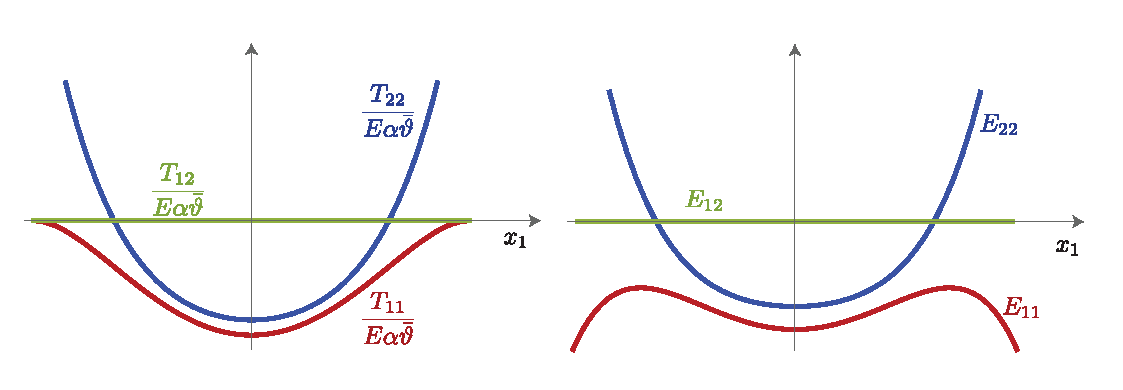
\includegraphics[scale=0.7]{figure/problema_elastico/rettangolo_termo}
		\end{centering}
		
	\end{svolgimento}
\end{exercise}





%\chapter{Plastic Materials}


%\section{Phenomenological Features of the Elastic-Plastic  Response}
%
%
%The fundamental characteristics of the elastic-plastic behavior of polycrystalline metals can be illustrated through the stress-strain curve obtained from a uniaxial tensile test. In such an experiment, a cylindrical sample with initial length $L_0$ and cross-sectional area $A_0$ is stretched to a new length $L$, resulting in an axial force $P$. The \emph{engineering stress} (or Piola stress), defined with respect to the undeformed area, is given by
%\[
%s = \frac{P}{A_0}.
%\]
%
%If $\lambda = L / L_0$ denotes the axial stretch ratio, then the associated \emph{engineering strain} is defined as
%\[
%e = \lambda - 1.
%\]
%
%\begin{figure}
%	\centering
%	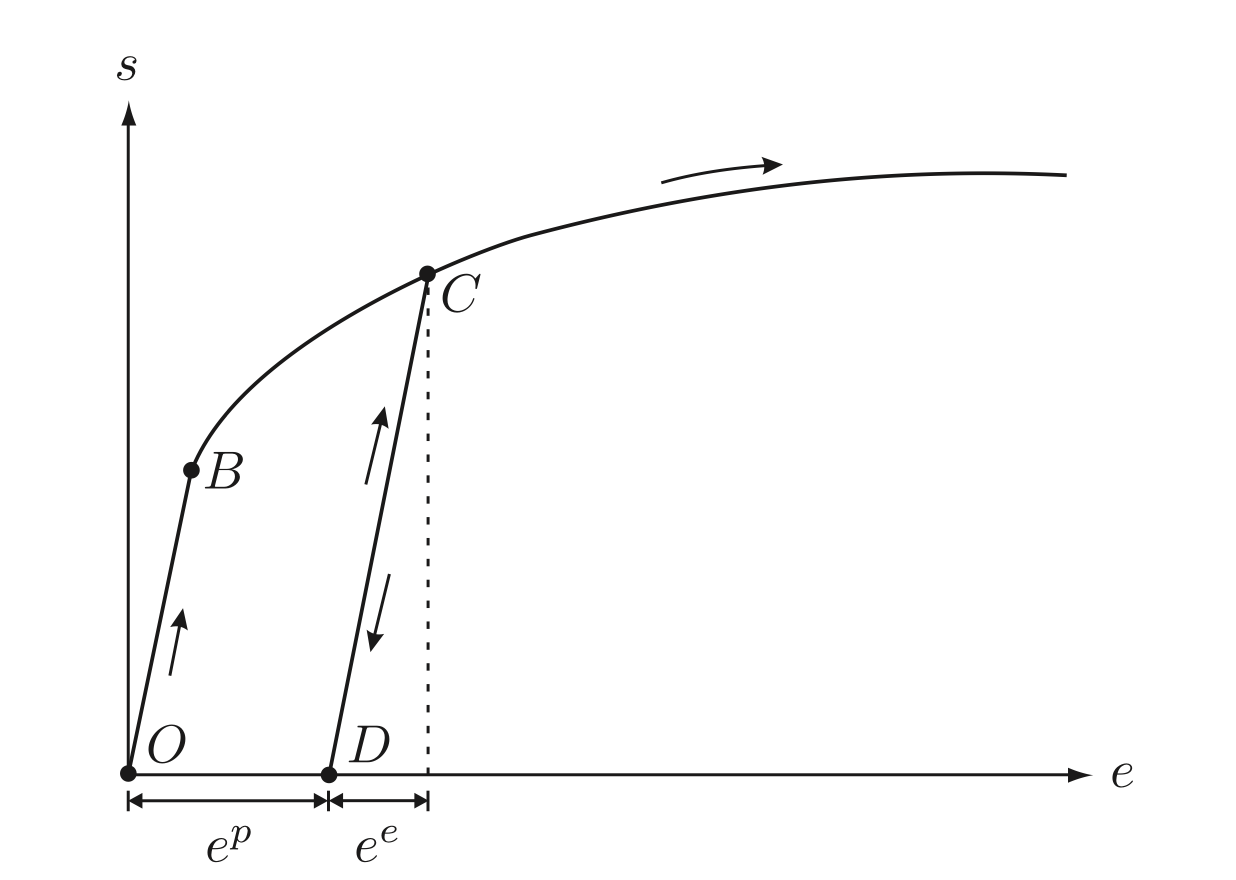
\includegraphics[width=0.6\linewidth]{figure/problema_elastico/plastic}
%	\caption{Schematic of an engineering stress-strain curve for a metallic material.}
%	\label{fig:plastic}
%\end{figure}
%
%A typical engineering stress versus strain curve for metals is presented in Fig. \ref{fig:plastic}; it shows an initial linear segment $OB$, representing elastic behavior. Reversing the loading path within this region results in a retraced path along the same line, indicating reversible deformation. The point $B$ marks the limit of linearity, known as the \emph{elastic limit}, and the corresponding stress is referred to as the \emph{yield strength}.
%
%Beyond the yield point, the curve departs from linearity, and stress continues to rise with increasing strain. This region corresponds to \emph{strain hardening}, where the material supports higher loads despite a decrease in cross-sectional area. This segment is often called the \emph{hardening curve}.
%
%If unloading begins from a point $C$ beyond the elastic regime, the stress does not follow the original loading path. Instead, the material unloads elastically along a different path $CD$, characterized by partial recovery of the deformation. The strain recovered during this stage is the \emph{elastic strain} $e^e$, while the remaining permanent strain is the \emph{plastic strain} $e^p$. A subsequent reloading from point $D$ typically returns along the unloading path, eventually rejoining the hardening curve at $C$, after which further loading continues along the existing hardening trajectory.
%
%In addition to engineering stress, one may also consider the \emph{true stress} (or Cauchy stress), which accounts for the instantaneous cross-sectional area $A$:
%\[
%\sigma = \frac{P}{A}.
%\]
%
%In addition to engineering strain, the \emph{true strain} (also referred to as logarithmic strain) is defined by the relation
%\[
%\epsilon = \ln \lambda.
%\]
%
%To determine the true stress during a tensile test, one must measure both the applied force $P$ and the instantaneous cross-sectional area $A$ of the specimen. Since concurrent measurements of elongation and lateral contraction are uncommon in typical tests, it is standard to assume that the plastic deformation of metals occurs at nearly constant volume (incompressibility). While elastic deformation involves volume changes, these are negligible compared to plastic effects.
%
%Under this assumption, the volume of the specimen remains approximately constant:
%\[
%A L \approx A_0 L_0.
%\]
%Using this, the true stress $\sigma$ and true strain $\epsilon$ can be related to engineering measures as:
%\[
%\sigma = \frac{P}{A} = \frac{P}{A_0} \cdot \frac{L}{L_0} = s(1 + e), \qquad \epsilon = \ln(1 + e).
%\]
%
%These expressions enable conversion from engineering stress and strain to their true counterparts.
%
%\vspace{1em}
%
%When true stress-strain curves from tension and compression tests are compared—both performed at ambient conditions—it is often observed that they nearly coincide for most metals. This indicates that the intrinsic plastic behavior of the material is independent of the type of loading. Conversely, engineering stress-strain curves for tension and compression often differ significantly due to the evolving geometry during deformation. Consequently, the \textit{true stress-strain curve is generally accepted as the most accurate representation of the material’s intrinsic plastic behavior}.
%
%\vspace{1em}
%\begin{figure}
%	\centering
%	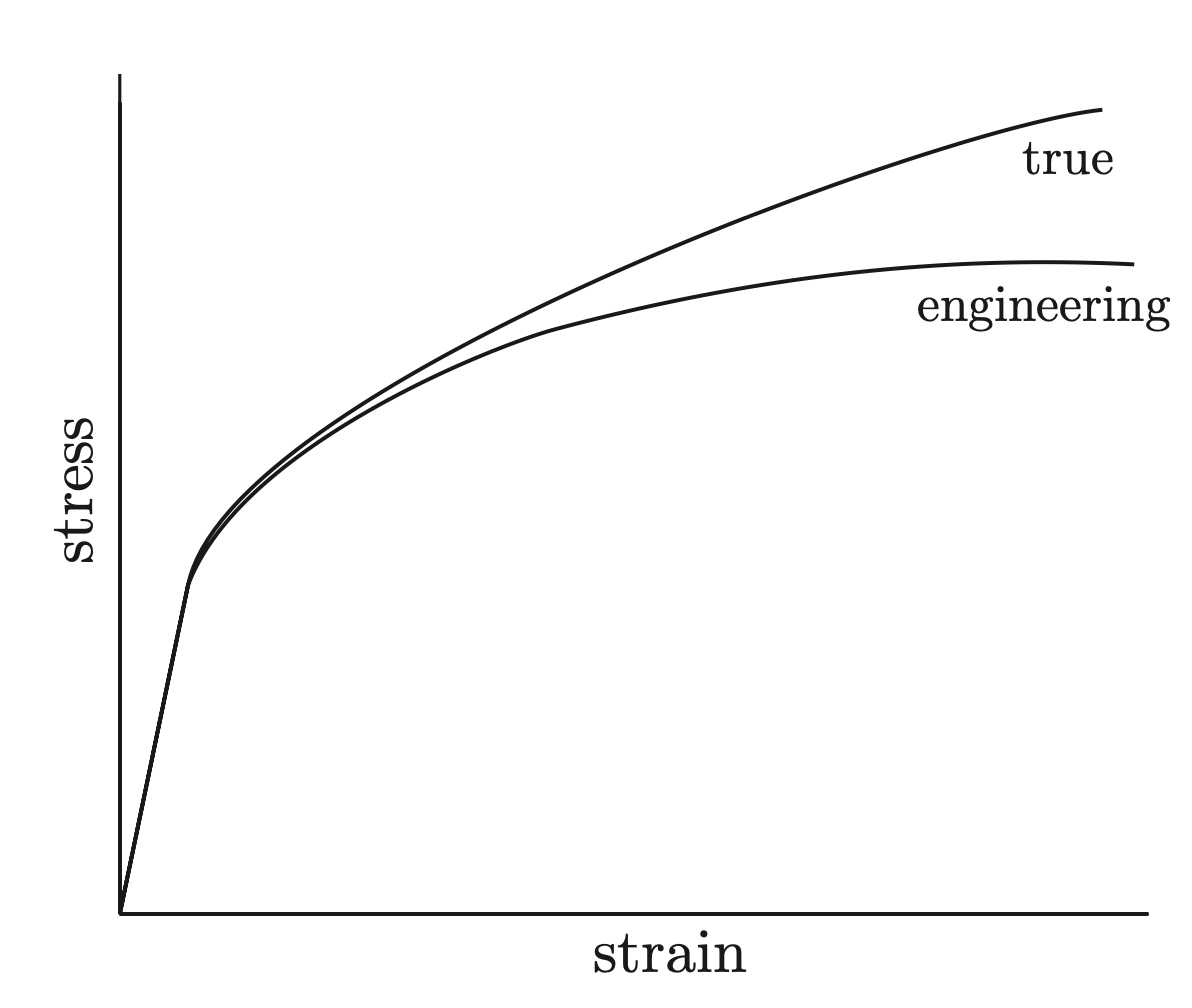
\includegraphics[width=0.5\linewidth]{figure/problema_elastico/plastic1}
%	\caption{Comparison of a true stress-strain curve with the corresponding engineering
%		stress-strain curve.}
%	\label{fig:plastic1}
%\end{figure}
%
%The mechanical behavior of metals under cyclic loading differs substantially from that under monotonic loading. One prominent feature observed is the \emph{Bauschinger effect}, initially described by Bauschinger in 1886. This effect refers to the reduction in yield stress upon load reversal: a metal specimen that has been plastically stretched shows a diminished resistance when subsequently compressed. 
%
%
%
%A schematic of such reversed-loading behavior is illustrated in Figure \ref{fig:plastic1}, where the solid line depicts the true stress-strain path of a sample first loaded in tension, followed by compression.
%
%\subsection*{74.1 Isotropic and Kinematic Strain-Hardening}
%
%As is clear from our brief discussion of the phenomenology of the stress-strain response, the deformation of metals beyond the elastic limit is quite complicated. In this subsection, we discuss some idealizations of strain-hardening that are frequently used in theories of plasticity.
%
%A simple idealization of actual material response, referred to as \textbf{isotropic hardening}, accounts for strain-hardening but approximates the hardening by a straight line, neglects the Bauschinger effect, and assumes that after reversal of deformation from any level of strain in the plastic regime, the magnitude of the flow stress upon which reverse yielding begins has the same value as the flow stress from which the unloading was initiated. The stress-strain response corresponding to isotropic hardening is shown schematically in Figure 74.4(a).
%
%Let the stress level from which reversed deformation is initiated be denoted by $\sigma_f$, and denote the stress at which the stress-strain curve in compression begins to deviate from linearity by $\sigma_r < 0$. The closed interval $[\sigma_r, \sigma_f]$ is called the \emph{elastic range}, and its endpoints $\{\sigma_r, \sigma_f\}$ are called the \emph{yield set}. Let $Y$, with initial value $Y_0$, denote the \emph{flow resistance} (a material property) of the material. The initial elastic range then has
%\[
%\sigma_r = -Y_0, \quad \sigma_f = Y_0,
%\]
%and, during subsequent plastic deformation along the hardening curve, the deformation resistance increases linearly from $Y_0$ to $Y$ due to strain-hardening, and the new elastic range becomes
%\[
%\sigma_r = -Y, \quad \sigma_f = Y.
%\]
%For such an idealized response of an elastic-plastic material, the magnitude of the stress $\sigma$ in this elastic range is bounded with the restriction
%\[
%|\sigma| \leq Y,
%\]
%generally referred to as a \emph{yield condition}, with plastic flow possible when $|\sigma| = Y$.
%
%Isotropic strain-hardening is an idealization of the actual hardening behavior of metals; in particular, it does not account for the Bauschinger effect. An alternative simple model for strain-hardening that accounts for this phenomenon is referred to as \textbf{kinematic hardening}. The stress-strain response for a material with linear kinematic hardening is shown in Figure 74.4(b): the initial flow resistance is $Y_0$; upon deformation in tension into the plastic regime, the stress increases linearly to $\sigma_f$, and, upon reversal of deformation, the material starts to plastically flow at a stress level $\sigma_r < 0$ and thereafter again continues to harden linearly. The magnitude $|\sigma_r|$ of the stress at which plastic flow recommences upon load reversal is smaller than that of $\sigma_f$, at which the reversed loading event was initiated — which embodies the \emph{Bauschinger effect}. The asymmetry in the onset of yield upon reversal of loading in such a model arises because of the buildup of an internal stress called the \emph{backstress} and denoted by $\sigma_b$, whose magnitude is equal to
%\[
%\sigma_b = \frac{1}{2} (\sigma_f + \sigma_r).
%\]
%
%The term \emph{kinematic hardening} reflects the fact that the center of the \emph{elastic range} in stress space moves from an initial value of $\sigma = 0$ to a value of $\sigma = \sigma_b$, while the height of the elastic range remains constant at $2Y_0$. This is in contrast to isotropic hardening shown in Figure 74.4(a), where the \emph{elastic range} in stress space stays centered at $\sigma = 0$, while the height of the elastic range expands from $2Y_0$ to $2Y$ as the material strain-hardens. For the material with kinematic hardening described above, the stress obeys the yield condition
%\[
%|\sigma - \sigma_b| \leq Y_0.
%\]
%
%For many metals, the actual strain-hardening behavior — including the Bauschinger effect — may be approximated by a combination of nonlinear isotropic hardening and nonlinear kinematic hardening.



\section{Kinematical Assumptions}
Most theories of plasticity are grounded in a physical intuition that envisions a plastic solid as possessing an underlying microscopic structure---such as a crystal lattice---that can undergo stretching and rotation, along with the presence of defects like dislocations that can move within this structure. In what follows, we give mathematical form to this perspective by introducing a kinematical constitutive assumption that requires the displacement gradient to admit the specific decomposition:
\begin{equation}
\nabla\ub=\He+\Hp,
\end{equation}
where
\begin{enumerate}
	\item $\He$ is the \textit{elastic distortion}, representing stretch and rotation of the underlying microscopic structure;
	\item $\Hp$ is the \textit{plastic distortion}, representing the local deformation of material due to 	the formation and motion of dislocations through that structure.
\end{enumerate}

Let us introduce the \textit{elastic} and \textit{plastic strains}
\begin{equation}
	\Ee=\sym\He, \qquad \Ep=\sym\Hp,
\end{equation}and the \textit{elastic} and \textit{plastic rotations}
\begin{equation}
	\We=\skw\He, \qquad \Wp=\skw\Hp,
\end{equation}
so that
\begin{equation}
\Eb=\Ee+\Ep, \qquad \Wb=\We+\Wb.
\end{equation}
Finally, consistent with the general observation that the flow of dislocations
does not induce changes in volume, we assume that $\Hp$ is deviatoric, \textit{i.e.}
\begin{equation}
\operatorname{tr} \Hp=\operatorname{tr}\Ep=0.
\end{equation}

In this presentation, we adopt the virtual-power formulation, proposed by Gurtin \cite{Gurtin_2003,Gurtin2}. 
What sets this approach unconventional is the inclusion of distinct internal power contributions related to both elastic and plastic responses. While this formulation aligns with traditional theory, it offers a useful framework for discussing material stability. Additionally, interpreting conventional theory within a virtual power framework lays the groundwork for developing theories that involve the \textit{gradient of plastic strain}.

This formulation is based on the idea that
 \textit{for every independent kinematical quantity of rate type, the associated power input can be described through a force system that satisfies its own balance equation.}

In this case the rate-like descriptors are not independent, since
\begin{equation}\label{constr}
\nabla\dot\ub=\dot\He+\dot\Hp, \qquad \operatorname{tr}\dot\Hp=0.
\end{equation}


We replace the classical expression for internal power $\Tb\cdot\nabla\dot\ub$, with a more refined decomposition that accounts separately for the distinct kinematical mechanisms at play, namely:
\begin{itemize}
	\item the elastic distortion rate $\dot\He$, which reflects the stretching of the microscopic structure, and
	\item the plastic distortion rate $\dot\Hp$, which captures the motion of dislocations within that structure.
\end{itemize}

Accordingly, we introduce:
\begin{itemize}
	\item an elastic stress  $\Te$, energetically conjugate to $\dot\He$, and
	\item a plastic stress $\Tp$, conjugate to $\dot\Hp$,
\end{itemize}
and express the internal power in the form:
\begin{equation}\label{intpPL}
\Wc^{\rm(int)}(\Pi)=\int_\Pi \Te\cdot\dot\He+\Tp\cdot\dot\Hp.
\end{equation}
Since $\dot\Hp$ is deviatoric, we may assume, without loss in generality, that 
\begin{equation}
\operatorname{tr}\Tp=0.
\end{equation}
The principle of virtual power is grounded in the condition that the internal and external power expenditures are in balance. We require that the \textit{power balance} holds:
\begin{equation}
\int_{\partial\Pi}\tb(\nb)\cdot\dot\ub+\int_\Pi\bb\cdot\dot\ub=\int_\Pi\Te\cdot\dot\He+\Tp\cdot\dot\Hp.
\end{equation}
We define a virtual velocity to be the list
\begin{equation}
\Uc=\{ \tilde\ub, \tilde\He, \tilde \Hp  \},
\end{equation}
and claim that the principle of virtual power is the requirement that
\begin{definition}
\begin{equation}\label{PVPpla}
\int_{\partial\Pi}\tb(\nb)\cdot\tilde\ub+\int_\Pi\bb\cdot\tilde\ub=\int_\Pi\Te\cdot\tilde\He+\Tp\cdot\tilde\Hb^{\rm p},
\end{equation}
\end{definition}
for all virtual velocities $\Uc$.

\subsection{Virtual Power and Frame-Indifference}

In Chap. \ref{PPV}, the classical principle of virtual power for large deformations was formulated through an internal power expenditure of the form
\begin{equation}
\int_{\Pi} \mathbf{T} \cdot \grad \tilde{\mathbf{v}}.
\end{equation}
The argument in Sec. \ref{symPVP}, ensuring the symmetry of \( \mathbf{T} \) and rewriting the integrand from \( \mathbf{T} \cdot\tilde{\mathbf{D}} \), relies on the frame-indifference requirement imposed on the internal power.

A similar reasoning applies here, but now starting from the internal power expression $\Wc^{\rm(int)}(\Pi)$ introduced in \eqref{intpPL}.

Specifically, frame-indifference for small deformations demands that the internal power $\Wc^{\rm(int)}(\Pi)$ remains invariant under transformations of the form:
\begin{definition}
	\begin{equation}\label{FIsmall}
	(\widetilde{\mathbf{H}}^{\rm e})^+ =\mathbf{H}^{\rm e} + \boldsymbol{\Omega}, \quad (\widetilde{\mathbf{H}}^{\rm p})^+= \mathbf{H}^{\rm p}, 
\end{equation}
\end{definition}
where \( \boldsymbol{\Omega} \) is any constant skew-symmetric tensor field. 
Indeed, within a linearized framework
\begin{equation}
\tilde\ub^+=\tilde\ub+\Omegab \,\xb,
\end{equation}
whence
\begin{equation}
\widetilde{\Hb}^+=\widetilde\Hb +\Omegab=(\widetilde{\Hb}^{\rm e}+\widetilde{\Hb}^{\rm p})+\Omegab.
\end{equation}
Now, plastic flow is an internal material rearrangement (sliding, dislocation, etc.), and rigid-body motion do not afffect internal material behavior. Therefore $\widehat{\Hb}^{\rm p}$ must be frame-indifferent, and then \eqref{FIsmall} follows.


This requirement leads to:
\[
\int_{\Pi} \mathbf{T}^{\rm e} \cdot (\widetilde{\mathbf{H}}^{\rm e} + \boldsymbol{\Omega})  = \int_{\Pi} \mathbf{T}^{\rm e} \cdot\widetilde{\mathbf{H}}^{\rm e} 
\]
for every region \( \Pi \) and every skew tensor \( \boldsymbol{\Omega} \). Therefore, \( \mathbf{T}^{\rm e} \) must necessarily be symmetric:
\begin{equation}\label{symTe}
\mathbf{T}^{\rm e} = (\mathbf{T}^{\rm e})^\top, 
\end{equation}
and hence
\[
\int_{\Pi} \mathbf{T}^{\rm e} \cdot\widetilde{\mathbf{H}}^{\rm e}  = \int_{\Pi} \mathbf{T}^{\rm e} \cdot \widetilde{\mathbf{E}}^{\rm e} 
\]

%\medskip
%
%\noindent \textbf{Remark.} The above reasoning, grounded in frame-indifference and establishing the symmetry of \( \mathbf{T} \) (i.e., \( \mathbf{T} = \mathbf{T}^{\rm e} \)), leads to the observation that the internal power can be expressed as
%\[
%\mathcal{I}(P) = \int_{\Pi} \left( \mathbf{T} : \dot{\mathbf{E}} + \cdots \right) , \tag{84.16}
%\]
%a structure that will hold throughout subsequent developments without further repetition.
%
%\bigskip

\subsection{Local Force Balances from Virtual Power}

The next task is to derive the local force balances implied by the principle of virtual power. When applying the power balance \eqref{PVPpla}, the virtual velocity field \( \mathcal{U} \) can be freely chosen under the constraint consequent to \eqref{constr}.

Consider a virtual velocity \( \mathcal{U} \) defined by an arbitrary \( \mathbf{u} \) such that:
\begin{equation}
	\widetilde{\mathbf{H}}^{\rm e} = \nabla \tilde{\mathbf{u}},
	\end{equation}
	so that $\widetilde{\mathbf{H}}^{\rm p}\equiv \mathbf{0}$.
For such virtual motions, the power balance \eqref{PVPpla} simplifies to:
\[
\int_{\partial \Pi} \mathbf{t}(\mathbf{n}) \cdot \tilde{\mathbf{u}}  + \int_{\Pi} \mathbf{b} \cdot \tilde{\mathbf{u}}  = \int_{\Pi} \mathbf{T}^{\rm e} \cdot\nabla \tilde{\mathbf{u}} ,
\]
involving only a single kinematic variable, namely the virtual velocity \( \tilde{\mathbf{u}} \) of material points. This justifies this virtual velocities  \emph{macroscopic}.

Next, by applying the divergence theorem, we obtain:
\[
\int_{\Pi} \mathbf{T}^{\rm e} \cdot \nabla\tilde{ \mathbf{u}} = - \int_{\Pi} \text{Div} \, \mathbf{T}^{\rm e} \cdot \tilde{\mathbf{u}} + \int_{\partial \Pi} (\mathbf{T}^{\rm e} \mathbf{n}) \cdot \tilde{\mathbf{u}} 
\]
and therefore, the power  balance  can be rewritten as:
\[
\int_{\partial \Pi} \left( \mathbf{t}(\mathbf{n}) - \mathbf{T}^{\rm e} \mathbf{n} \right) \cdot \tilde{\mathbf{u}}  + \int_{\Pi} \left( \text{Div} \, \mathbf{T}^{\rm e} + \mathbf{b} \right) \cdot \tilde{\mathbf{u}}  = 0.
\]
Since the domain \( \Pi \) and the virtual velocity \( \tilde{\mathbf{u}} \) are arbitrary, the fundamental lemma of the calculus of variations implies the the traction condition
\begin{equation}
	\mathbf{t}(\mathbf{n}) = \mathbf{T}^{\rm e} \mathbf{n}, 
\end{equation}
and the  local force balance
\begin{definition}
\begin{equation}\label{balTe}
	\text{Div} \, \mathbf{T}^{\rm e} + \mathbf{b} = \mathbf{0}
\end{equation}
\end{definition}

These two relations, together with the symmetry condition \eqref{symTe}, are the classical conditions satisfied by the standard Cauchy stress tensor. Therefore, we can identify:
\begin{definition}
\[
\mathbf{T} \equiv \mathbf{T}^{\rm e},
\]
\end{definition}
where \( \mathbf{T} \) denotes the \textit{macroscopic stress tensor}. Accordingly, \eqref{balTe} represents the \textit{macroscopic local balance of forces}.  This terminology is appropriate because its derivation of  was based solely on the macroscopic virtual velocities \( \mathcal{U} \). 

%Consequently, combining \eqref{84.4}, \eqref{84.22}, and \eqref{84.21} leads to the momentum balance equation:
%\[
%\text{Div} \, \mathbf{T} + \mathbf{b}_0 = \rho \ddot{\mathbf{u}}. \tag{84.23}
%\]

\medskip

We now demonstrate that,  in this framework, 	an additional force balance emerges, related specifically to the plastic stress \( \mathbf{T}^{\rm p} \).


To derive this new balance law, consider a virtual velocity field characterized by a deviatoric tensor \( \widetilde{\mathbf{H}}^{\rm p} \), with the elastic part given by:
\[
\widetilde{\mathbf{H}}^{\rm e} = -\widetilde{\mathbf{H}}^{\rm p}, 
\]
and with
\[
\tilde{\mathbf{u}} \equiv \mathbf{0}, 
\]
in agreement with \eqref{constr}.

These virtual velocities are termed \emph{microscopic} because they involve no macroscopic motion of the body as a whole. Rather, they represent purely local changes in shape caused by plastic flow, balanced by internal stretching and rotation of the material microstructure.

Substituting into the virtual work principle \eqref{PVPpla}, the power balance reads:

\begin{equation}\label{vpbal}
	\int_{\Pi} \left( \mathbf{T}^{\rm p} - \mathbf{T} \right) \cdot \widetilde{\mathbf{H}}^{\rm p}  = 0.
\end{equation}

Since, \( \mathbf{T}^{\rm p} \) is deviatoric, and since \( \widetilde{\mathbf{H}}^{\rm p} \) is also deviatoric, we  infer that \( \mathbf{T} \cdot \widetilde{\mathbf{H}}^{\rm p} = \dev \Tb \cdot \widehat{\mathbf{H}}^{\rm p} \), where \( \dev \Tb \) is the deviatoric part of \( \mathbf{T} \). 

As \( \Pi \) is arbitrary, the integrand must vanish, leading to the local condition:
\[
\left( \mathbf{T}^{\rm p} - \dev \Tb \right) \cdot \widetilde{\mathbf{H}}^{\rm p} = 0.
\]

If we take \( \widetilde{\mathbf{H}}^{\rm p} = \widetilde{\mathbf{W}}^{\rm p} \), an arbitrary skew tensor, then, since \( \mathbf{T} \) is symmetricwe get  \( \mathbf{T}^{\rm p} \cdot \widetilde{\mathbf{W}}^{\rm p} = 0 \) for all skew \( \widetilde{\mathbf{W}}^{\rm p} \), so that \( \mathbf{T}^{\rm p} \) is symmetric:
\[
\mathbf{T}^{\rm p} = (\mathbf{T}^{\rm p})^\top, 
\]
and  also deviatoric. Finally, since the deviatoric tensor field \( \widetilde{\mathbf{H}}^{\rm p} \)  is arbitrary, we are led to the 
\begin{definition}
\textbf{\textit{Microscopic force balance}}:
\begin{equation}\label{micrbal}
	\dev \Tb = \mathbf{T}^{\rm p}. 
\end{equation}
\end{definition}
This may be seen as a balance between
\begin{itemize}
	\item forces described by the \textit{macroscopic stress} \( \mathbf{T} \) and associated with the material structure, and
	\item forces described by the\textit{ microscopic stress} \( \mathbf{T}^{\rm p} \) and associated with the system of dislocations.
\end{itemize}

Finally, we note that — as a consequence of the symmetriesof the stresses \( \mathbf{T}^{\rm e} \) and \( \mathbf{T}^{\rm p} \), together with the identification \( \mathbf{T}^{\rm e} = \mathbf{T} \) — the power balance becomes
\[
\underbrace{\int_{\partial \Pi} \mathbf{t}(\mathbf{n}) \cdot \dot{\mathbf{u}} + \int_\Pi \mathbf{b} \cdot \dot{\mathbf{u}}}_{\mathcal{W}^{\rm (ext)}(\Pi)}
=
\underbrace{\int_\Pi \left( \mathbf{T} \cdot \dot{\mathbf{E}} + \mathbf{T}^{\rm p} \cdot \dot{\mathbf{E}}^{\rm p} \right)}_{\mathcal{W}^{\rm (int)}(\Pi)}. 
\]


\begin{remark}
The virtual power formulation enables a simple generalization of the conventional theory to cases where the\textit{ gradients of plastic strai}n and its \textit{rate} are treated as independent constitutive variables. It is hard to envision how such a generalization could arise from a traditional formulation of the theory.
\end{remark}




\section{ Codirectionality constraint: von Mises Plasticity}

We now develop a more restrictive form of the virtual-power principle by requiring — from the outset — that the \textit{codirectionality constraint}%
be satisfied.

In \textit{von Mises plasticity}, the codirectionality constraint refers to the requirement that the plastic strain rate tensor $\dot{\mathbf{E}}^{\rm p}$ must be proportional (\textit{i.e.}, codirectional) to the deviatoric part of the stress tensor $\dev \Tb$:
\begin{equation}
\label{codir}
\frac{\dev \Tb}{|\dev \Tb|} =\frac{\dot{\mathbf{E}}^{\rm p}}{|\dot{\mathbf{E}}^{\rm p}|}= :\mathbf{N}^{\rm p}
\end{equation}
The devitatoric tensor $\Nb^{\rm p}$ is the \textit{(plastic) flow direction}.

The von Mises theory models materials that are isotropic and incompressible during plastic flow (like metals at moderate temperatures). It says that yielding depends only on the deviatoric part of the stress (the part that causes distortions, not volume changes). Now, the codirectionality constraint says that when the material yields, the rate at which it plastically deforms (i.e., how the shape changes irreversibly) happens in the same direction as the distortional stress. The deviatoric stress $\dev \Tb$ is what tries to distort (shear, stretch sideways) the material without changing its volume; the material responds plastically directly along that effort: it plastically deforms exactly along the direction of the applied shear efforts.

\begin{remark}
A defininig property of a plastic solid is its ability to \textit{flow like a fluid}. We notice that the constitutive equation for the extra stress $\dev \Tb$ as a function of the stretching $\Db$ in an \textit{incompressible Newtonian fluid} has the simple form
\begin{equation}
	\dev \Tb=2\mu \Db,
\end{equation}
where $\mu$ is the shear modulus. It threfore satisfies the condition
\begin{equation}
\frac{\dev \Tb}{|\dev \Tb|}=\frac{\Db}{|\Db|}.
\end{equation}
\end{remark}

%Thus, necessarily, \( \mathbf{T} (\equiv \mathbf{T}^{\rm e}) \) is symmetric, consistent with frame-indifference.\footnote{%
%	Frame-indifference demands that observable quantities not depend on rigid body motions.
%}

By the codirectionality constraint, we can rewrite \( \dot{\mathbf{E}}^{\rm p} \) in the form
\[
\dot{\mathbf{E}}^{\rm p} = \dot{e}^{\rm p} \mathbf{N}^{\rm p}
\quad \text{and} \quad
\dot{e}^{\rm p} = |\dot{\mathbf{E}}^{\rm p}| \geq 0.
\]

The scalar $\dot{e}^{\rm p} $ is called the \textit{ plastic strain-rate}. It measures the instantaneous intensity of plastic deformation, independently of its direction, and is defined as the norm of the plastic strain-rate tensor. Its value is non-negative, and it vanishes when the material deforms elastically. Integrating  $\dot{e}^{\rm p} $ over time gives the \textit{accumulated  plastic strain}, namely
\begin{definition}
	\begin{equation}
e^{\rm p}=\int_0^t\dot{e}^{\rm p} (\tau)\,\dd \tau,
\end{equation}
\end{definition}
which measures the total amount of irreversible plastic deformation experienced by the material up to the current time. While $\dot{e}^{\rm p} $ quantifies the instantaneous rate at which plastic flow occurs, $e^{\rm p}$ summarizes the \textit{cumulative history} of plastic deformation in a single scalar quantity. The notion of accumulated plastic strain is due to Hill.

We therefore have that
\[
\dot{\mathbf{H}}^{\rm p} = \dot{e}^{\rm p} \mathbf{N}^{\rm p} + \dot{\mathbf{W}}^{\rm p}
\quad \text{and} \quad
\dot{\mathbf{W}}^{\rm p} = \mathrm{skw}\, \dot{\mathbf{H}}^{\rm p},
\]
where \( \dot{\mathbf{W}}^{\rm p} \) is the plastic spin. The kinematical constraint \eqref{constr} then takes the form
\[
\nabla \dot{\mathbf{u}} = \dot{\mathbf{H}}^e + \dot{e}^{\rm p} \mathbf{N}^{\rm p} + \dot{\mathbf{W}}^{\rm p}. \tag{84.33}
\]


We introduce the definitions
\[
\tau^{\rm p}= \mathbf{N}^{\rm p}\cdot \mathbf{T}^{\rm p}, \quad \text{and} \quad \mathbf{T}^{\rm p}_{\text{skw}} = \operatorname{skw} \mathbf{T}^{\rm p},
\]
and apply them to the balance of  power,  with \( \mathbf{T} \equiv \mathbf{T}^{\rm e} \) symmetric. We obtain:
\[
\int_{\partial \Pi} \mathbf{t}(\mathbf{n}) \cdot \dot{\mathbf{u}}  + \int_\Pi \mathbf{b} \cdot \dot{\mathbf{u}} \ = \int_\Pi \left( \mathbf{T} \cdot \dot{\mathbf{E}} + \tau^{\rm p}\dot{\varepsilon}^{\rm p}+ \left( \operatorname{skw} \mathbf{T}^{\rm p}\right) \cdot\dot{\mathbf{W}}^{\rm p}\right).
\]
We consider virtual fields \( \dot{\mathbf{u}} \), \( \dot{\mathbf{H}}^{\rm e} \), and \( \dot{\mathbf{H}}^{\rm p} \), satisfying the kinematic relation
\[
\nabla \dot{\mathbf{u}} = \dot{\mathbf{H}}^{\rm e} + \dot{\mathbf{H}}^{\rm p}, \quad \text{with} \quad \operatorname{tr} \dot{\mathbf{H}}^{\rm p} = 0.
\]
Differently from previous assumptions, we now impose that the plastic flow direction \( \mathbf{N}^{\rm p}\) is constrained by the codirectionality condition (84.31)\(_1\). Consequently, the space of admissible virtual plastic strain rates is restricted to fields of the form
\[
\dot{\mathbf{E}}^{\rm p}= \dot{\varepsilon}^{\rm p}\mathbf{N}^{\rm p}, \quad \dot{\varepsilon}^{\rm p}\geq 0,
\]
where:
\begin{itemize}
	\item[(i)] The virtual accumulated plastic strain-rate \( \dot{\varepsilon}^{\rm p}\) is nonnegative but otherwise arbitrary;
	\item[(ii)] The flow direction \( \mathbf{N}^{\rm p}\) is prescribed by the codirectionality constraint and is not an independent variation.
\end{itemize}

On this basis, we define the generalized virtual velocity list:
\[
\mathcal{U} = \left( \tilde{\mathbf{u}}, \widetilde{\mathbf{H}}^{\rm e}, \tilde{\varepsilon}^{\rm P}, \widetilde{\mathbf{W}}^{\rm p}\right),
\]
subject to the  kinematic compatibility:
\[
\nabla \tilde{\mathbf{u}} = \widetilde{\mathbf{H}}^{\rm e} + \underbrace{ \tilde{\varepsilon}^{\rm p}\mathbf{N}^{\rm p}}_{\widetilde{\mathbf{H}}^{\rm p}} + \widetilde{\mathbf{W}}^{\rm p}.
\]
Given that \( \mathbf{T} \cdot \widetilde{\mathbf{E}} = \mathbf{T} \cdot\widetilde{\mathbf{H}}^{\rm e} \), we rewrite the external and internal power expenditures respectively as:
\[
\mathcal{W}^{\rm (ext)}(\Pi) [\mathcal{U}]= \int_{\partial \Pi} \mathbf{t}(\mathbf{n}) \cdot \tilde{\mathbf{u}}  + \int_\Pi \mathbf{b} \cdot \tilde{\mathbf{u}},
\]
and
\[
\mathcal{W}^{\rm (int)}(\Pi)[\mathcal{U}] = \int_\Pi  \mathbf{T} \cdot\widetilde{\mathbf{H}}^{\rm e} + \tau^{\rm p}\tilde{\varepsilon}^{\rm p}+ \left( \operatorname{skw} \mathbf{T}^{\rm p}\right) \cdot \widetilde{\mathbf{W}}^{\rm p}.
\]
The principle of virtual power asserts that, for every virtual velocity field \( \mathcal{U} \) and every subregion \( \Pi \),
\begin{definition}
	\[
\int_{\partial \Pi} \mathbf{t}(\mathbf{n}) \cdot \tilde{\mathbf{u}}  + \int_\Pi \mathbf{b} \cdot \tilde{\mathbf{u}}= \int_\Pi  \mathbf{T} \cdot\widetilde{\mathbf{H}}^{\rm e} + \tau^{\rm p}\tilde{\varepsilon}^{\rm p}+ \left( \operatorname{skw} \mathbf{T}^{\rm p}\right) \cdot \widetilde{\mathbf{W}}^{\rm p}.
\]
\end{definition}
Moreover, the same arguments leading to the local balance of forces apply, yielding:
\[
\operatorname{Div} \mathbf{T} + \mathbf{b} = \mathbf{0}.
\]

In order to derive the microscopic force banalce, we consider the microscopic virtual velocity
\begin{equation}
\widetilde{\Hb}^{\rm e}=-(\tilde{e}^{\rm p}\Nb^{\rm p}+\widetilde{\Wb}^{\rm p}), \qquad \tilde{\ub}=\mathbf{0};
\end{equation}
as a consequence, since$\Tb\cdot\widetilde{\Wb}^{\rm p}=0$,
\begin{equation}
\int_\Pi (\tau^{\rm p}-\Tb\cdot\Nb^{\rm p})\,\tilde{e}^{\rm p}+(\skw \Tb^{\rm p})\cdot\widetilde{\Wb}^{\rm p}=0.
\end{equation}
But both $\Pi$ and $\widetilde{\Wb}^{\rm p}$ are abitrary; thus $\skw \Tb^{\rm p}=\mathbf{0}$ and
\begin{equation}
	(\tau^{\rm p}-\Tb\cdot\Nb^{\rm p})\,\tilde{e}^{\rm p}=0.
\end{equation}
Finally, since $\tilde{e}^{\rm p}\geq 0$ is arbitrary, and since $\Nb^{\rm p}\cdot\dev \Tb=|\dev \Tb|$, we have the microscopic force balance
\begin{definition}
	\begin{equation}
|\dev \Tb|=\tau^{\rm p}.
\end{equation}
\end{definition}


%\section{Virtual External forces associated with dislocation flow}
%As we will see, we find it convenient to allow for external \textit{microscopic} forces associated with the flow of dilocations through the body. Since such flows are characterize by the plastic strain-rate $\dot{\Eb}^{\rm p}$, we introduce an arbitrary symmetric and deviatoric external microscopic force $\Bb^{\rm p}$ power-conjugated to $\dot{\Eb}^{\rm p}$, and hence the external power has to be expanded as follows:
%\begin{equation}
%	\Wc^{\rm (ext)}=\int_{\partial\Pi}\tb(\nb)\cdot \dot{\ub}+\int_{\Pi}\bb\cdot\dot{\ub}+\int_\Pi\Bb^{\rm p}\cdot\dot{\Eb}^{\rm p}
%\end{equation}
%It would not seem a simple matter to produce the external microscopic force $\Bb^{\rm p}$ in the laboratory; for that reason $\Bb^{\rm p}$ should be considered as virtual.
%
%The inclusion of $\Bb^{\rm p}$ allows for physically meaningful ``thought experiments'' that we will use to motivate a precise notion of material stability. Specifically,
%we consider the external microscopic force $\Bb^{\rm p}$  as a test force applied by an external
%agency to evolve the system of dislocations via the power expenditure $\Bb^{\rm p}\cdot\dot{\Eb}^{\rm p}$, an
%expenditure that — when positive — serves as an indication of the stability of the
%system with $\Bb^{\rm p}=\mathbf{0}$. Further, because we account for the power expended by $\Bb^{\rm p}$,
%this force is also useful in determining thermodynamically consistent constitutive
%relations for $\Te$ and $\Tp$.

\section{Virtual External Forces Associated with Dislocation Flow}

To develop a consistent framework for dislocation-mediated plasticity, it is helpful to extend the principle of virtual power to include not only conventional (macroscopic) forces but also \emph{virtual microscopic forces} that act on the internal mechanisms of plastic deformation.

In particular, since plastic flow is described at the macroscopic level by the \emph{plastic strain-rate} $\dot{\mathbf{E}}^{\rm p}$, we introduce a \emph{symmetric and deviatoric virtual microscopic force} $\mathbf{B}^{\rm p}$, which is defined to be \emph{power-conjugate} to $\dot{\mathbf{E}}^{\rm p}$. This means that the scalar quantity $\mathbf{B}^{\rm p} \cdot \dot{\mathbf{E}}^{\rm p}$ represents the power expended by this force to produce a given plastic flow.

Accordingly, the total external power functional becomes:
\begin{equation}
	\mathcal{W}^{\rm (ext)} = \int_{\partial \Pi} \mathbf{t}(\mathbf{n}) \cdot \dot{\mathbf{u}} 
	+ \int_{\Pi} \mathbf{b} \cdot \dot{\mathbf{u}} 
	+ \int_\Pi \mathbf{B}^{\rm p} \cdot \dot{\mathbf{E}}^{\rm p}
\end{equation}
where the last term represents the power input due to the virtual microscopic force.


The microscopic force $\mathbf{B}^{\rm p}$ is not physically realizable in an experiment—it cannot be directly applied in the laboratory. Instead, it is introduced as a \emph{virtual test force}, used to probe the internal response of the system. It allows us to construct \emph{energetically motivated thought experiments}, which provide insight into the nature of \emph{material stability}, as we will see.

In this context, we imagine applying $\mathbf{B}^{\rm p}$ in a chosen direction of plastic flow. If, for every such direction, the virtual force must do positive work (i.e., $\mathbf{B}^{\rm p} \cdot \dot{\mathbf{E}}^{\rm p} > 0$), then we say the system is \emph{materially stable}: plastic flow does not occur spontaneously, and any attempt to initiate it requires energy input. In this sense, the system is protected by an \emph{energetic barrier}.

Moreover, by tracking the virtual power expended by $\mathbf{B}^{\rm p}$, we gain a powerful tool for deriving hermodynamically consistent constitutive relations for both the \emph{ macrostress} $\mathbf{T}^{\rm e}$ and the \emph{ microstress} $\mathbf{T}^{\rm p}$, which govern the evolution of dislocations.

If we admit the presence of $\Bb^{\rm p}$, the microscopic force balance \eqref{micrbal} is replaced by
\begin{definition}
\begin{equation}\label{micrbal1}
	 \mathbf{T}^{\rm p}-\dev \Tb=\Bb^{\rm p}. 
\end{equation}
\end{definition}

\section{Free-energy imbalance}

Since our current treatment of force relies on a  framework based on nonclassical ideas of stress and power, it becomes necessary to formulate an appropriate version of the free-energy imbalance, distinct from the traditional one. Guided by this objective, we impose the following principle:

\begin{definition}
	For any arbitrary subregion \( \Pi \), the rate of change of free energy within \( \Pi \) must equal the mechanical power input to \( \Pi \) minus the internal dissipation, with the dissipation being nonnegative.
\end{definition}

Letting \( \psi \) denote the free energy density and \( \delta \geq 0 \) the dissipation per unit volume, this principle leads to the \textit{free-energy imbalance}:
\[
\int_\Pi \dot{\psi}  = \underbrace{ \int_{\partial \Pi} \mathbf{t}(\mathbf{n}) \cdot \dot{\mathbf{u}}  + \int_\Pi \mathbf{b} \cdot \dot{\mathbf{u}}  }_{\mathcal{W}^{\rm (ext)}(\Pi)} - \int_\Pi \delta ,
\]
where \( \mathcal{W}^{\rm (ext)}(\Pi) \) represents the external mechanical power expended on \( \Pi \).

By invoking the mechanical power balance, we can rewrite the above equation as:
\[
\int_\Pi \dot{\psi}  = \int_\Pi \left( \mathbf{T} \cdot \dot{\mathbf{E}} + \mathbf{T}^{\rm p} \cdot \dot{\mathbf{E}}^{\rm p} \right)  - \int_\Pi \delta .
\]

Since \( \Pi \) is arbitrary, we deduce the local form of the free-energy imbalance:
\begin{definition}
	\[
\dot{\psi} - \mathbf{T} \cdot \dot{\mathbf{E}} - \mathbf{T}^{\rm p} \cdot\dot{\mathbf{E}}^{\rm p} = -\delta \leq 0.
\]
\end{definition}



In the specific case where the codirectionality condition holds, we have
\[
\mathbf{T}^{\rm p} : \dot{\mathbf{E}}^{\rm p} = \tau^{\rm p} \dot{\varepsilon}^{\rm p},
\]
where \( \dot{\varepsilon}^{\rm p} \) is the accumulated plastic strain rate.

Thus, the local free-energy imbalance reduces to:
\begin{definition}
	\begin{equation}\label{fePLA}
\dot{\psi} - \mathbf{T} : \dot{\mathbf{E}} - \tau^{\rm p} \dot{\varepsilon}^{\rm p} = -\delta \leq 0.
	\end{equation}
\end{definition}

\section{Constitutive Theory}
We assume that defect energy can be neglected and that the material response separates cleanly into elastic and plastic contributions. Consequently, motivated by the local free-energy imbalance, we adopt the following constitutive framework:
\begin{equation}\label{constPLA}
	\psi = \widehat{\psi}(\mathbf{E}^{\rm e}), \qquad \mathbf{T} = \widehat{\mathbf{T}}(\mathbf{E}^{\rm e}), \qquad \mathbf{T}^{\rm p} = \widehat{\mathbf{T}}^{\rm p}(\dot{\mathbf{E}}^{\rm p}, e^{\rm p}),
\end{equation}
where \( \mathbf{E}^{\rm e} \) denotes the elastic strain and \( e^{\rm p} \) is the accumulated plastic strain, introduced to model \textit{hardening} effects.

\begin{remark}
 The accumulated plastic strain  \( e^{\rm p} \) is treated as an \textit{ internal variable} that characterizes the evolution of the material’s microstructure during plastic deformation, accounting for irreversible phenomena such as the increase in dislocation density. In the formulation of constitutive models, the stress is expressed as a function of the current strain-rate and the current internal variables, and not of their rates of change. This structure ensures that the material response depends on the present state, which inherently reflects the entire history of past plastic deformations through the value of  \( e^{\rm p} \).
\end{remark}

\subsection{Rate-Independence}
Let us define a change in time scale:
\begin{equation}\label{transft}
	t^+=\kappa t,
\end{equation}
where $\kappa>0$ is the \textit{rate} constant of the transformation. Given an abitrary function $\varphi$ of the time, under the transformation \eqref{transft}, it transforms to the function $\varphi_\kappa$, with
\begin{equation}
\varphi_k(t)=\varphi(\kappa t),
\end{equation}
so that, by the chain rule,
\begin{equation}
\dot \varphi_\kappa=\kappa \dot\varphi(\kappa t)
\end{equation}

We assume that the material is \textit{rate-independent}, or, rather better, that the constitutive equation \eqref{constPLA}$_3$ is rate-identependent. Under the time-scale change \eqref{transft} this equation becomes
\begin{equation}
\Tb^{\rm p}_\kappa(t)=\widehat{\Tb}^{\rm p}\Big(\dot\Eb_\kappa^{\rm}(t), e_\kappa^{\rm p}(t)  \Big)=\widehat{\Tb}^{\rm p}\Big(\kappa\dot\Eb^{\rm}(t), e^{\rm p}(\kappa t)  \Big)
\end{equation}
Therefore, omitting the argument $\kappa t$, we must have
\begin{equation}\label{ratind}
 \widehat{\mathbf{T}}^{\rm p}(\dot{\mathbf{E}}^{\rm p})= \widehat{\mathbf{T}}^{\rm p}(\kappa\dot{\mathbf{E}}^{\rm p})
\end{equation}
and, since the rate constant $\kappa$ is arbitrary, this euqality must hold for all $\kappa>0$, and all $\dot{\Eb}^{\rm p}$ and $e^{\rm p}$.

Let us choose $\dot{\Eb}^{\rm p}\neq 0$ arbitrarily and choose a reference flow-rate $d_0$ and take $\kappa=\frac{d_0}{|\dot{\Eb}^{\rm p}|} $; by \eqref{ratind}, the response function $\widehat{\mathbf{T}}^{\rm p}(\dot{\mathbf{E}}^{\rm p}, e^{\rm p})$ must have the form
\begin{equation}
	\widehat{\mathbf{T}}^{\rm p}(\dot{\mathbf{E}}^{\rm p}, e^{\rm p})=	\widehat{\mathbf{T}}^{\rm p}\left(d_0\frac{\dot{\Eb}^{\rm p}}{|\dot{\Eb}^{\rm p}|} , e^{\rm p}\right).
\end{equation}
Thus, redefining $	\widehat{\mathbf{T}}^{\rm p}$ to absorb the constant $d_0$, we see that the most general rate-independent constitutive realtion of the form \eqref{constPLA}$_3$  must have the specific form
	\begin{equation}
\Tb^{\rm p}=\widehat{\mathbf{T}}^{\rm p}\left(\frac{\dot{\Eb}^{\rm p}}{|\dot{\Eb}^{\rm p}|} , e^{\rm p}\right),
\end{equation}
 or rather 
\begin{definition}
	\begin{equation}\label{constTp}
		\Tb^{\rm p}=\widehat{\mathbf{T}}^{\rm p}\left(\Nb^{\rm p} , e^{\rm p}\right).
	\end{equation}
\end{definition}
Since $\frac{\dot{\Eb}^{\rm p}}{|\dot{\Eb}^{\rm p}|}$ is defined only when $\dot \Eb^{\rm p}\neq \mathbf{0}$, the constitutive equation \eqref{constTp} is defined only when $\dot \Eb^{\rm p}\neq \mathbf{0}$, \textit{i.e.}, when there is \textit{plastic flow}.


In the limit \( \dot{\mathbf{E}}^{\rm p} = \mathbf{0} \), we treat \( \mathbf{T}^{\rm p} \) as indeterminate, and the microscopic balance equation $\mathbf{T}^{\rm p} = \dev \Tb$
is automatically satisfied.

We call the pair $(\dev\Tb, \Nb^{\rm p})$  a \textit{normalized flow}. A normalized flow is physically attainable if and only if $\dev\Tb$ and $\Nb^{\rm p}$ are related through the
 the microforce balance \eqref{micrbal}, which, with the constitutive equation \eqref{constTp}, becomes the
\begin{definition}
\textbf{\textit{Flow rule}}\\
\begin{equation}
	\dev \Tb=\widehat{\mathbf{T}}^{\rm p}\left(\Nb^{\rm p} , e^{\rm p}\right).
\end{equation}
\end{definition}

\subsection{Thermodynamics restrictions}


The presence of the external body force $\Bb^{\rm p}$ (as well as the conventional body
force $\bb$) allows us to use the Coleman–Noll procedure to ensure compatibility of constitutive assumptions with the free-energy imbalance \eqref{fePLA}. 

Consider a constitutive process with $\dot\Eb^{\rm p}=\mathbf{0}$. Then the free-energy imbalance \eqref{fePLA} reduces to $\dot\psi\leq \Tb\cdot\dot\Eb^{\rm e}$, an equality satisfied in all such constitutive processes only if $\Tb=\partial_{\Eb}\psi$, a result that reduces \eqref{fePLA} to $\Tb^{\rm p}\cdot \dot\Eb^{\rm p}\geq 0$.

The request that \eqref{fePLA}  hold in all constitutive processes yield the following thermodynamics restrictions:
\begin{definition}
	\begin{equation}\label{threstr}
\widehat{\Tb}(\Eb^{\rm e})=\partial_{\Eb}\widehat{\psi}(\Eb^{\rm e}), \qquad \widehat{\Tb}^{\rm p}(\Nb^{\rm p}, e^{\rm p})\cdot \dot\Eb^{\rm p}\geq 0.
\end{equation}
\end{definition}

\section{Material Stability}
The force balance \eqref{micrbal1} is accompanied by an associated power balance
\begin{definition}
	\begin{equation}\label{micrpow}
	(\Tb^{\rm p}-\dev\Tb)\cdot\dot{\Eb}^{\rm p}=\Bb^{\rm p}\cdot \dot{\Eb}^{\rm p},
\end{equation}
\end{definition}
where $\Bb^{\rm p}\cdot \dot{\Eb}^{\rm p}$ represents the power epended by the external agency. Let us divide the microscopic power balance \eqref{micrpow} by $\dot{\Eb}^{\rm p}$
(assumed strictly positive):
\begin{equation}
\Bb^{\rm p}\cdot \Nb^{\rm p}=(\Tp-\dev\Tb)\cdot \Nb^{\rm p}.
\end{equation}
%The notion of material stability is based on the balance \eqref{micrbal1}, and for that reason we work with the constituive relation
%\begin{equation}\label{consteqTp}
%\Tp=\widehat{\Tb}^{\rm p}(\Nb^{\rm p}, e^{\rm p})
%\end{equation}
%for the plastic stress $\Tp$. In so doing
%\begin{enumerate}
%	\item $\Tp$ always denotes the plastic stress; as such it is related to the flow direction Np
%	through the constitutive relation \eqref{consteqTp};
%	\item $\dev \Tb$ always denotes the deviatoric macroscopic stress; as such it is arbitrary.
%\end{enumerate} 
%We use the term \textit{normalized flow} for a pair $(\dev\Tb, \Nb^{\rm p})$ with $\dev\Tb$ a (macroscopic deviatoric) stress and $\Nb^{\rm p}$ a flow direction.
%For $(\dev\Tb, \Nb^{\rm p})$  such a flow and $\Tb$, the plastic stress corresponding to $\Nb^{\rm p}$, the
%external force $\Bb^{\rm p}$ computed via \eqref{micrbal1} represents a force exerted by an external
%agency in support of the normalized flow  $(\dev\Tb, \Nb^{\rm p})$.
%
%In this case, we refer to a normalized flow $(\dev\Tb, \Nb^{\rm p})$ as \textit{physically attainable} if the
%external force needed to support it vanishes, \textit{i.e.}
%\begin{equation}
%	\Bb^{\rm p}=\mathbf{0}.
%\end{equation}
%
%Thus, $(\dev\Tb, \Nb^{\rm p})$ physically attainable if and only if $\dev\Tb$ and $\Nb^{\rm p}$ are related through the flow rule
%\begin{equation}\label{flowrule}
%	\dev \Tb=\widehat{\mathbf{T}}^{\rm p}\left(\Nb^{\rm p} , e^{\rm p}\right).
%\end{equation}
%
%Hence, physically attainable flows — that is, flows that do not require a virtual external
%microscopic power-expenditure — are possible when and only when the deviatoric macroscopic stress $\det\Tb$ and the flow direction $\Nb^{\rm p}$ are related through the flow
%rule \eqref{flowrule}.
%
%The only flows that one might see in actual experiments are those that are
%physically attainable and hence consistent with the flow rule. More generally, the
%presence of an external agency as represented by the external force $\Bb^{\rm p}$ allows us
%to at least contemplate ``thought experiments”'' involving normalized flows $(\dev\Tb, \Nb^{\rm p})$
%that are not compatible with the flow rule.
%
%Specifically, given such a flow $(\dev\Tb, \Nb^{\rm p})$, we consider $\Bb^{\rm p}\cdot\Nb^{\rm p}$ as a test
%expenditure of power applied by the external agency to investigate the stability of
%the normalized flow $(\dev\Tb, \Nb^{\rm p})$ — and we note that conventional notions of \textit{material
%stability}.
%
%In particular, Drucker\footnote{See Drucker, D.C., 1964. On the postulate of stability of material in the mechanics of
%	continua. Journal de Mechanique 3, 235–250} focuses on external macroscopic forces and ensures that the material cannot spontaneously gain energy during loading cycles.
%	The forces applied by the external agency are introduced by incrementing the
%	standard macroscopic forces.
%
%This notion would then imply that if
%	\begin{equation}\label{stab}
%	\Bb^{\rm p}\cdot\Nb^{\rm p}>0 \quad \textrm{for all $\Nb^{\rm p}$}
%	\end{equation}
%then the external agency expends power for flow in any direction; in this case
%there is an energetic barrier for flow and the ``system'' is stable; as we wish to
%include neutral stability in our notion of stability, we replace \eqref{stab} by
%\begin{equation}\label{stab1}
%	\Bb^{\rm p}\cdot\Nb^{\rm p}\geq0 \quad \textrm{for all $\Nb^{\rm p}$}.
%\end{equation}
%The following definition — based on the foregoing bullet and the power balance
%\eqref{micrpow} — is central to what follows. A deviatoric stress $\dev\Tb$ is \textit{materially stable} if
%\begin{equation}
%(\widehat{\Tb}^{\rm p}(\Nb^{\rm p},e^{\rm p})-\dev\Tb)\cdot\dot{\Nb}^{\rm p}\geq0 \quad \textrm{for every flow drection $\Nb^{\rm p}$}.
%\end{equation}
%Thus $\dev\Tb$ is materially stable if and only if, given any flow direction $\Nb^{\rm p}$, plastic flow
%in the direction of $\Nb^{\rm p}$ requires a nonnegative expenditure of power by an external
%agency.
%
%The \textit{flow resistance} is defined as
%\begin{equation}
%Y(\Nb^{\rm p}, e^{\rm p})=\widehat{\Tb}^{\rm p}(\Nb^{\rm p},e^{\rm p})\cdot\Nb^{\rm p}
%\end{equation}
%
%Therefore, a stress $\dev\Tb$ is materially stable if and only if 
%\begin{equation}
%\dev\Tb\cdot \Nb^{\rm p}\leq Y(\Nb^{\rm p}, e^{\rm p})\quad \textrm{for every flow drection $\Nb^{\rm p}$}.
%\end{equation}
%
The notion of material stability is grounded in the microscopic balance
\eqref{micrbal1}, and for this reason we adopt the constitutive relation
\begin{equation}\label{consteqTp}
	\Tp = \widehat{\Tb}^{\rm p}(\Nb^{\rm p}, e^{\rm p})
\end{equation}
for the plastic stress $\Tp$. This implies the following conventions:
\begin{enumerate}
	\item $\Tp$ always denotes the plastic stress, which is determined by the flow direction $\Nb^{\rm p}$ via the constitutive relation \eqref{consteqTp};
	\item $\dev \Tb$ always denotes the deviatoric part of the macroscopic stress and is treated as arbitrary.
\end{enumerate}

We define a \emph{normalized flow} as a pair $(\dev\Tb, \Nb^{\rm p})$, where $\dev\Tb$ is a deviatoric stress and $\Nb^{\rm p}$ a flow direction. For such a pair, the external microscopic force $\Bb^{\rm p}$ computed through \eqref{micrbal1} represents the virtual force required by an external agency to sustain the flow $(\dev\Tb, \Nb^{\rm p})$.

A normalized flow $(\dev\Tb, \Nb^{\rm p})$ is said to be \emph{physically attainable} if the external microscopic force vanishes:
\begin{equation}
	\Bb^{\rm p} = \mathbf{0}.
\end{equation}
This occurs if and only if the stress and flow direction are related by the flow rule:
\begin{equation}\label{flowrule}
	\dev \Tb = \widehat{\Tb}^{\rm p}(\Nb^{\rm p}, e^{\rm p}).
\end{equation}

Thus, flows that do not require any virtual power input from an external agency (i.e., physically attainable flows) are precisely those consistent with the flow rule \eqref{flowrule}. Only such flows are expected to occur in real experiments.

The introduction of a virtual external force $\Bb^{\rm p}$, however, enables thought experiments involving flows that do \emph{not} satisfy the flow rule. For such hypothetical flows $(\dev\Tb, \Nb^{\rm p})$, we interpret the scalar quantity
\[
\Bb^{\rm p} \cdot \Nb^{\rm p}
\]
as the power input required from an external agency to enforce the flow direction $\Nb^{\rm p}$ under the stress $\dev\Tb$. This leads us to a stability criterion.

Following Drucker,\footnote{D.C. Drucker (1964), \emph{On the postulate of stability of material in the mechanics of continua}, Journal de Mécanique, 3, 235–250.} who formulated stability in terms of macroscopic loading cycles, we propose an analogous microscopic condition: if
\begin{equation}\label{stab}
	\Bb^{\rm p} \cdot \Nb^{\rm p} > 0 \quad \text{for all } \Nb^{\rm p},
\end{equation}
then the external agency must expend power for any possible flow direction, implying that the system resists all plastic deformation. This reflects a strict notion of stability, where an energetic barrier opposes all flow.

To allow for neutral stability (i.e., zero net power input), we adopt the weaker condition
\begin{equation}\label{stab1}
	\Bb^{\rm p} \cdot \Nb^{\rm p} \geq 0 \quad \text{for all } \Nb^{\rm p}.
\end{equation}

We are now ready to state a key definition: a deviatoric stress $\dev\Tb$ is said to be \emph{materially stable} if
\begin{equation}
	\left( \widehat{\Tb}^{\rm p}(\Nb^{\rm p}, e^{\rm p}) - \dev\Tb \right) \cdot \Nb^{\rm p} \geq 0 \quad \text{for all flow directions } \Nb^{\rm p}.
\end{equation}
In other words, $\dev\Tb$ is materially stable if, for any plastic flow direction $\Nb^{\rm p}$, the external agency must supply a nonnegative amount of power to support that flow.

We define the \emph{flow resistance} as
\begin{equation}
	Y(\Nb^{\rm p}, e^{\rm p}) = \widehat{\Tb}^{\rm p}(\Nb^{\rm p}, e^{\rm p}) \cdot \Nb^{\rm p}.
\end{equation}
Then, a stress $\dev\Tb$ is materially stable if and only if
\begin{definition}
	\begin{equation}
	\dev\Tb \cdot \Nb^{\rm p} \leq Y(\Nb^{\rm p}, e^{\rm p}) \quad \text{for all flow directions } \Nb^{\rm p}.
\end{equation}
\end{definition}

Usually the \textit{strong isotropy} hypothesis is enforced, \textit{i.e.} the flow resistance is assumed to be independent of the flow direction $\Nb^{\rm p}$:
\begin{equation}
Y(\Nb^{\rm p}, e^{\rm p}) =Y(e^{\rm p}).
\end{equation}

If the co-directionality hypothesis is enforced, we have the condition
\begin{definition}
	\begin{equation}
	|\dev\Tb|\leq Y(e^{\rm p})
\end{equation}
\end{definition}

The \textit{elastic range} is the set
\begin{equation}
\Ec(e^{\rm p})=\textrm{the set of all $\dev\Tb$ such that $|\dev\Tb|\leq Y(e^{\rm p})$}.
\end{equation}

The \textit{yield set}  is given by
\begin{equation}
\mathcal{Y}(e^{\rm p})=\textrm{the set of all $\dev\Tb$ such that $|\dev\Tb|= Y(e^{\rm p})$}=\partial\Ec(e^{\rm p}).
\end{equation}

The following statements are true:
\begin{enumerate}
	\item Given any flow stress $\dev\Tb$, the flow direction $\Nb^{\rm p}$ corresponding to $\dev\Tb$ is the out-
	ward unit normal to $\mathcal{Y}$ at $\dev\Tb$.
	\item The yield set is strictly convex.
	\item The elastic range $\Ec$ is the closed, bounded region whose boundary is $\mathcal{Y}$ and for
	which the flow direction is directed outward from $\mathcal{E}$.
	\item The interior of the elastic range is the set of all stresses $\dev\Tb$ that are strictly admissible  and	
	$	\dot{\Eb}^{\rm p}$  throughout the interior of the elastic range.
	\end{enumerate}
These are results of the so-called \textit{Drucker's theorem}, whose proof we omit.

The central results of the theory, summarized as follows, define the Mises theory of rate-independent plastic response:
\begin{definition}
\begin{equation}\label{Mis}
\begin{aligned}
&\dev \Tb=Y(e^{\rm p})\frac{\dot{\Eb}^{\rm p} }{|\dot{\Eb}^{\rm p}|}\quad \textrm{for $\dot{\Eb}^{\rm p}\neq \mathbf{0}$} \quad&& \textrm{(Mises flow rule)},\\
&e^{\rm p}=|\dot{\Eb}^{\rm p}| \quad && \textrm{(hardening equation)},\\
&|\dev \Tb|\leq Y(e^{\rm p}) && \textrm{(boundedness inequality)},\\
&\dot{\Eb}^{\rm p}=\mathbf{0} \quad \textrm{for $\dev\Tb<Y(e^{\rm p})$} &&  \textrm{(no-flow condition)}.\\
\end{aligned}
\end{equation}
\end{definition}

By \eqref{threstr} the dissipation associated with the Mises plasticity is 
\begin{definition}
	\begin{equation}\label{dissPL}
\delta=Y(e^{\rm p} )|\dot{\Eb}^{\rm p}|.
\end{equation}
\end{definition}

We remark that the flow rule \eqref{Mis}$_1$ is a (microforce) balance equation endowed with a constitutive equation for the plastic stress $\Tp$:
\begin{equation}
\widehat{\Tb}^{\rm p}(\Nb^{\rm p}, e^{p})=Y(e^{\rm p})\Nb^{\rm p}.
\end{equation}

\begin{remark}
Effective theories of rate-independent plasticity typically start with the concept of a \textit{yield surface} — a closed surface in SymDev — and define the elastic range as the subset of SymDev bounded by the yield surface. In this context, the concept of stability offers a framework that is significantly more comprehensive than the classical approach, leading to natural definitions for both the elastic range and the yield surface.
\end{remark}


\begin{remark}
In the plasticity literature, analogous results can be deduced by appealing to  the concept of \textit{maximum dissipation} is  a well-established idea. It provides a convenient and effective means of modeling the evolution of plastic deformation by linking it directly to the dissipation of energy. However, this framework, while useful, often remains somewhat abstract and is treated as an assumption or an axiom, rather than being derived from more fundamental principles. In contrast, the notion of material stability, which we advocate here, offers a more robust and compelling foundation for understanding plasticity. Unlike the concept of maximum dissipation, material stability is not merely introduced as a postulate. Instead, it emerges from a rigorous theoretical argument rooted in the principle of virtual power, which is a more general and versatile framework. This allows for a deeper, more systematic exploration of the behavior of materials under loading, with a direct connection to classical concepts of stability.
\end{remark}


\section{Variational formulation of the flow rule}
Variational inequalities serve as a fundamental framework for formulating, analyzing, and solving initial and boundary value problems in rate-independent plasticity. Essentially, they act as the counterpart to the first variation in minimization problems, playing a role analogous to that of the virtual power principle in relation to force balance equations. Moreover, they offer a weak formulation of the governing equations—``weak'' in the sense that the required regularity of the solution is reduced, and the equations are satisfied in a global sense. Such weak formulations are also the foundation for finite element methods. In what follows, we first reformulate the Mises flow equations in terms of dissipation

\medskip

Let us choose $\dev\Tb, \dot{\Eb}^{\rm p}$ and a scalar $e^{\rm p}$. Then $\dev\Tb, \dot{\Eb}^{\rm p}$ and  $e^{\rm p}$ satisfy the flow rule \eqref{Mis}$_1$ and the boundedness inequality 
 \eqref{Mis}$_3$ if and only if they satisfy the 
\begin{definition}
\textbf{\textit{Local inequality} (LI)}
	 \begin{equation}\label{LI}
 	\delta(\widetilde{\Eb}^{\rm p}, e^{\rm p})\geq \delta(\dot{\Eb}^{\rm p}, e^{\rm p})+\dev\Tb\cdot(\widetilde{\Eb}^{\rm p}-\dot{\Eb}^{\rm p}) \quad \textrm{ for all symmetric and deviatoric $\widetilde{\Eb}^{\rm p}$.}
 \end{equation}
\end{definition}
The proof is achieved by steps. The accumulated plastic strain $e^{\rm p}$ is fixed and, for sake of conciseness we omit is as an argument.

We now assume $\dot{\Eb}^{\rm p}\neq\mathbf{0}$ and show that
\begin{enumerate}
	\item\textit{ the Mises flow rule  \eqref{Mis}$_1$ implies the local inequality \eqref{LI}.}
	
	If is satisfied, from \eqref{dissPL} we get 
	\begin{equation}
	\begin{aligned}
			Y^{-1} \big[\delta(\widetilde{\mathbf{E}}^{\rm p}) - \delta(\dot{\mathbf{E}}^{\rm p}) - \dev\Tb \cdot (\widetilde{\mathbf{E}}^{\rm p} - \dot{\mathbf{E}}^{\rm p})\big] 
		&= |\widetilde{\mathbf{E}}^{\rm p}| - |\dot{\mathbf{E}}^{\rm p}| - \frac{\dot{\mathbf{E}}^{\rm p}}{|\dot{\mathbf{E}}^{\rm p}|} \cdot (\widetilde{\mathbf{E}}^{\rm p} - \dot{\mathbf{E}}^{\rm p})\\
	&= |\widetilde{\mathbf{E}}^{\rm p}| - \frac{\dot{\mathbf{E}}^{\rm p}}{|\dot{\mathbf{E}}^{\rm p}|} \cdot \widetilde{\mathbf{E}}^{\rm p} \\
	&= \frac{1}{|\dot{\mathbf{E}}^{\rm p}|}( |\widetilde{\mathbf{E}}^{\rm p}| |\dot{\mathbf{E}}^{\rm p}|- \widetilde{\mathbf{E}}^{\rm p}\cdot\dot{\mathbf{E}}^{\rm p})
	\end{aligned}
	\end{equation}
	By the Cauchy–Schwarz inequality, we know that
	\[
	\dot{\mathbf{E}}^{\rm p} \cdot \widetilde{\mathbf{E}}^{\rm p} \leq |\dot{\mathbf{E}}^{\rm p}| \, |\widetilde{\mathbf{E}}^{\rm p}|,
	\]
	which guarantees that the right-hand side of the expression above is nonnegative. Therefore,  \eqref{Mis}$_1$ implies  \eqref{LI}.
\item 	We now prove the converse: \textit{  the local inequality \eqref{LI} implies the Mises flow rule  \eqref{Mis}$_1$.}
 
 To this end, we use \eqref{dissPL} to rewrite inequality \eqref{LI} in the form:
	\begin{equation}\label{eq:ineq-converse}
		Y(|\widetilde{\mathbf{E}}^{\rm p}| - |\dot{\mathbf{E}}^{\rm p}|) \geq \dev\Tb \cdot (\widetilde{\mathbf{E}}^{\rm p} - \dot{\mathbf{E}}^{\rm p}) \quad \text{for all } \widetilde{\mathbf{E}}^{\rm p} \in \text{SymDev}.
	\end{equation}
	
	Now, choose $\widetilde{\mathbf{E}}^{\rm p}$ such that $|\widetilde{\mathbf{E}}^{\rm p}| = |\dot{\mathbf{E}}^{\rm p}|$, divide both sides of \eqref{eq:ineq-converse} by $|\dot{\mathbf{E}}^{\rm p}|$, and define the normalized tensors
	\[
	\mathbf{N}^{\rm p} = \frac{\dot{\mathbf{E}}^{\rm p}}{|\dot{\mathbf{E}}^{\rm p}|}, \qquad \widetilde{\mathbf{N}}^{\rm p} = \frac{\widetilde{\mathbf{E}}^{\rm p}}{|\dot{\mathbf{E}}^{\rm p}|}.
	\]
	Then inequality \eqref{eq:ineq-converse} becomes
	\begin{equation}\label{eq:ineq-converse1} 
		\dev\Tb \cdot (\widetilde{\mathbf{N}}^{\rm p} - \mathbf{N}^{\rm p}) \leq 0. 
	\end{equation}
	
	Next, let $\bm\Lambda \in \text{SymDev}$ be any deviatoric tensor satisfying the orthogonality condition
	\begin{equation}
		\bm\Lambda \cdot\mathbf{N}^{\rm p} = 0. 
	\end{equation}
	
	Let $\mathcal{N}$ denote the unit sphere in the space of deviatoric symmetric tensors. There exists a smooth curve $\widetilde{\mathbf{N}}^{\rm p}(\lambda)$ on $\mathcal{N}$ such that, for some $\lambda_0$,
	\begin{equation}\label{Lam}
		\widetilde{\mathbf{N}}^{\rm p}(\lambda_0) = \mathbf{N}^{\rm p}, \qquad \left.\frac{d\widetilde{\mathbf{N}}^{\rm p}(\lambda)}{d\lambda}\right|_{\lambda = \lambda_0} = \bm\Lambda,
	\end{equation}
	 and such that, by \eqref{eq:ineq-converse1}  and \eqref{Lam}$_1$, the function
\begin{equation}
	\Phi(\lambda) = \dev\Tb\cdot (\widehat{\Nb}^{\rm p}(\lambda) - \Nb^{\rm p}) \leq 0 
\end{equation}
has a maximum at $\lambda = \lambda_0$. Consequently,
\[
\left. \frac{d\Phi(\lambda)}{d\lambda} \right|_{\lambda = \lambda_0} = \dev\Tb\cdot \left. \frac{d\widehat{\Nb}^{\rm p}(\lambda)}{d\lambda} \right|_{\lambda = \lambda_0} = 0,
\]
so that, by \eqref{Lam},
\begin{equation}\label{beta}
	\dev\Tb \cdot\bm\Lambda = 0 
\end{equation}
for every $\bm\Lambda \in \mathrm{SymDev}$ tangent to $\mathcal{N}$ at $\Nb^{\rm p}$. The stress $\dev\Tb$ must therefore be normal to $\mathcal{N}$ at $\Nb^{\rm p}$; there is hence a scalar $\beta$ such that
\begin{equation}
	\dev\Tb= \beta \Nb^{\rm p}.
\end{equation}

Next, to show that $\beta = Y$, we first take $\widetilde{\Eb}^{\rm p} = \mathbf{0}$. Then, by \eqref{beta} and, since
\[
\Nb^{\rm p} \cdot \dot{\Eb}^{\rm p} = |\dot{\Eb}^{\rm p}|,
\]
\eqref{eq:ineq-converse} becomes $Y|\dot{\Eb}^{\rm p}| \leq \beta |\dot{\Eb}^{\rm p}|$; consequently,
\begin{equation}
	Y \leq \beta.
\end{equation}

On the other hand, assume that $\Nb^{\rm p} = \widetilde{\Nb}^{\rm p}$. Then, $\Nb^{\rm p} \cdot \widetilde{\Eb}^{\rm p} = |\widetilde{\Eb}^{\rm p}|$ and \eqref{eq:ineq-converse} becomes
\[
Y(|\widetilde{\Eb}^{\rm p}| - |\dot{\Eb}^{\rm p}|) \geq \beta (|\widetilde{\Eb}^{\rm p}| - |\dot{\Eb}^{\rm p}|),
\]
so that $Y \geq \beta$. Thus, $Y = \beta$ and then the flow rule $\dev\Tb = Y \Nb^{\rm p}$ is satisfied. 
\end{enumerate}

\bigskip
\noindent Let us now assume  that
\begin{equation}
	\dot{\Eb}^{\rm p} = \mathbf{0};
\end{equation}
we have to show that
\begin{enumerate}
	\item \textit{  The local inequality \eqref{LI}, and then \eqref{eq:ineq-converse}, implies the boundedness inequality \eqref{Mis}$_3$}.
Since $\dot{\Eb}^{\rm p}=\mathbf{0}$,   \eqref{eq:ineq-converse} becomes
\begin{equation}
	Y |\widetilde{\Eb}^{\rm p}| \geq \dev\Tb \cdot \widetilde{\Eb}^{\rm p} \quad \text{for all } \widetilde{\Eb}^{\rm p} \in \mathrm{SymDev}.
\end{equation}

Dividing by $|\widetilde{\Eb}^{\rm p}|$ and then choosing $\widetilde{\Eb}^{\rm p} = \dev\Tb$, we find that

\begin{equation}\label{eq:ineq-converse2}
	Y \geq \dev\Tb\cdot \frac{\dev\Tb}{\dev|\Tb|} = |\dev\Tb|,
\end{equation}

which is the boundedness inequality  \eqref{Mis}$_3$. 

\item  \textit{The boundedness inequality \eqref{Mis}$_3$ implies the local inequality \eqref{eq:ineq-converse}}.
 Choose $\widetilde{\Eb}^{\rm p} \in \mathrm{SymDev}$ arbitrarily. Then,\eqref{Mis}$_3$ and the Schwarz inequality imply that
\[
Y |\widetilde{\Eb}^{\rm p}| \geq |\dev\Tb||\widetilde{\Eb}^{\rm p}| \geq \dev\Tb\cdot \widetilde{\Eb}^{\rm p},
\]
which is \eqref{eq:ineq-converse2}. This completes the proof.

\end{enumerate}
%
%\subsection{The global variational inequality}
%We now proceed to derive the global variational inequality appropriate for problems involving the Mises flow equations. Without loss of generality, we substitute $\dev\Tb$ in \eqref{LI} with $\Tb$. Suppose that the displacement $\ub$ and the fields $\dot{\Eb}^{\rm p}$, $e^{\rm p}$, $\Tb$, and $\widetilde{\Eb}^{\rm p}$ are defined over $\Omega$ (with $e^{\rm p}$ compatible with \eqref{dissPL}, and $\widetilde{\Eb}^{\rm p}$ an arbitrary tensor in $\mathrm{SymDev}$). Define the functional
%\begin{align}
%	\Jc(\widetilde{\Eb}^{\rm p}, e^{\rm p}) &= \int_{\Omega} \delta(\widetilde{\Eb}^{\rm p}, e^{\rm p}) = \int_{\Omega} Y(e^{\rm p}) |\widetilde{\Eb}^{\rm p}|\
%\end{align}
%where we have used relation  \eqref{dissPL}. Recalling the linear elastic stress-strain law
%\begin{equation}
%	\Tb = \mathbb{C}(\sym \nabla \ub - \Eb^{\rm p}) \tag{82.20}
%\end{equation}
%with $\mathbb{C}$ denoting the elasticity tensor, we integrate \eqref{LI} over $\Omega$ to obtain
%\begin{equation}
%	J(\widetilde{\Eb}^{\rm p}, e^{\rm p}) \geq J(\dot{\Eb}^{\rm p}, e^{\rm p}) + \int_{\Omega} (\widetilde{\Eb}^{\rm p} - \dot{\Eb}^{\rm p}) : \mathbb{C} \Eb^{\rm e} \, dv, \tag{82.21}
%\end{equation}
%where the elastic strain is defined as
%\begin{equation}
%	\Eb^{\rm e} := \sym \nabla \ub - \Eb^{\rm p}.
%\end{equation}
%
%We now consider boundary conditions of the form
%\begin{equation}
%	\Tb \nb = \sb \quad \text{on } \partial_N\Omega, \qquad \ub = \mathbf{0} \quad \text{on } \partial_D \Omega,
%\end{equation}
%where $\sb$ is a prescribed surface traction on a subset $\partial_N\Omega$ of $\partial \Omega$. In the following, we consider only virtual fields that are kinematically admissible, i.e., such that
%\begin{equation}
%	\widetilde{\vb} = \mathbf{0} \quad \text{on } \partial_D \Omega.
%\end{equation}
%
%Using the symmetry of $\Tb$, the virtual power identity takes the form
%\begin{equation}
%	\int_{\Omega} \Tb : \nabla \widetilde{\vb}\, dv = \int_{\partial_N\Omega} \sb \cdot \widetilde{\vb}\, da + \int_{\Omega} \bb \cdot \widetilde{\vb}\, dv \tag{82.25}
%\end{equation}
%and holds for all kinematically admissible virtual displacements $\widetilde{\vb}$ if and only if
%\begin{equation}
%	\Div \Tb + \bb = \mathbf{0} \quad \text{in } \Omega, \qquad \Tb \nb = \sb \quad \text{on } \partial_N\Omega. \tag{82.26}
%\end{equation}
%
%We may now, without loss of generality, substitute $\widetilde{\vb}$ in \eqref{82.25} with $\widetilde{\ub} - \ub$, where $\widetilde{\ub}$ is kinematically admissible. Using \eqref{82.20}, this leads to
%\begin{equation}
%	\int_{\partial_N\Omega} \sb \cdot (\widetilde{\ub} - \ub)\, da + \int_{\Omega} \bb \cdot (\widetilde{\ub} - \ub)\, dv + \int_{\Omega} (\sym \nabla \widetilde{\ub} - \sym \nabla \ub) : \mathbb{C} \Eb^{\rm e}\, dv = 0. \tag{82.27}
%\end{equation}






\part{Appendices}
\setcounter{chapter}{0}
\chapter{Elements of algebra and tensor analysis}

%\addcontentsline{toc}{chapter}{A. Richiami di algebra ed analisi} % Aggiunge il capitolo all'indice
%\renewcommand{\theequation}{A\arabic{equation}}
%\setcounter{equation}{0} % Reset del contatore delle equazioni
\renewcommand{\thesection}{A.\arabic{section}}
\setcounter{section}{0} % Reset del contatore delle sezioni



% Ridefinisci la numerazione delle equazioni per questo capitolo
\renewcommand{\theequation}{A\arabic{equation}}
\setcounter{equation}{0} % Reset del contatore delle equazioni

\section{Vectors}  
We work in a Euclidean space $\Ec^n$ of dimension $n=1,2,3$; when $n$ is not explicitly indicated, we assume $n=3$. The elements of $\Ec$ are points $P$, $Q$, $\ldots$. The difference between two points is a vector, an element of the translation space $\Vc$ associated with $\Ec$:
\begin{equation}
	P-Q=\vb \in \Vc.
\end{equation}
$\Vc$ is a \textit{vector space}.

We will denote vectors with bold lowercase letters, generally Latin, but sometimes, when needed, we will also use Greek characters, $\ab, \bb, \ldots \boldsymbol{\alpha}, \boldsymbol{\beta}, \ldots$

Given a point $O$ in $\Ec^n$, the \textit{position vector} of $X$ with respect to $O$ can be written as
\begin{equation}
	P-O=\overrightarrow{OP}=\pb\in \Vc^n.
\end{equation}
For simplicity, we will sometimes refer to the point $\pb\in \Vc$, thinking of its position with respect to the origin.

We endow $\Vc$ with a \textit{scalar product}, denoted by $\ub\cdot \vb$, $\ub$, $\vb\in\Vc$.  
The \textit{norm} of a vector $\ub$ is $|\ub|\coloneqq \sqrt{\ub\cdot\ub}$. Let $\vartheta$ be the angle formed between two vectors $\ub$, $\vb$; we then have
\begin{equation}
	\ub \cdot \vb =|\ub||\vb|\cos \vartheta.
\end{equation}

A unit vector, or \textit{versor}, is a vector of norm 1, while two nonzero vectors are said to be \textit{orthogonal} if their scalar product is zero.

If $\Vc$ has dimension $n$, it is always possible to find an orthonormal system of $n$ vectors, which we will identify as a \textit{basis} of $\Vc$; we will choose one and denote it by $\eb_1, \eb_2, \ldots \eb_n$. We then have
\begin{equation}
	\eb_i \cdot \eb_j=\delta_{ij}, \qquad \forall i,j=1,2,\ldots, n,
\end{equation}
where $\delta_{ij}$ is the \textit{Kronecker delta} ($\delta=1$ if $i=j$ and 0 otherwise).

The components of a vector $\ub$ with respect to the basis $\{\eb_i\}$ are the scalars
\begin{equation}
	u_i=(\ub)_i\coloneqq \ub \cdot \eb_i.
\end{equation}
and therefore
\begin{equation}
	\ub =u_1 \eb_1+ u_2\eb_2+\ldots+u_n \eb_n=\sum_{i=1}^n u_i \eb_i.
\end{equation}
We will use the \textit{Einstein convention}: any index repeated twice in an expression is summed over all the possible values the index can take; thus, we can simply write
\begin{equation}
	\ub=u_i \eb_i
\end{equation}

If $n=3$, we can define the \textit{vector product} between two vectors $\ub$ and $\vb$:
\begin{equation}
	\ub \times \vb =(\ub \times \vb)_k \eb_k, \qquad (\ub \times \vb)_k=(u_i \eb_i)\times (b_j\eb_j)\cdot \eb_k=\epsilon_{ijk}a_i b_j,
\end{equation}
where 
\begin{equation}\label{Ricci}
	\epsilon_{ijk}=
	\begin{cases}
		\begin{aligned}
			&1 \qquad &&\text{if }(i,j,k)\text{ is an even permutation of }(1,2,3);\\
			&-1  &&\text{if }(i,j,k)\text{ is an odd permutation of }(1,2,3);\\
			&0 &&\text{if two indices are equal,}&
		\end{aligned}
	\end{cases}
\end{equation}
is the \textit{Ricci symbol}.

The Ricci symbol and the Kronecker delta are related by the equation
\begin{equation}\label{epsdel}
	\epsilon_{ijk}\epsilon_{ipq}=\delta_{jp}\delta_{kq}-\delta_{jq}\delta_{kp}.
\end{equation}

The product $\ub\times \vb$ is a vector orthogonal to both $\ub$ and $\vb$, with magnitude equal to the area of the parallelogram with sides $\ub$ and $\vb$, that is,
\begin{equation}
	|\ub \times \vb|=|\ub||\vb|\sin\vartheta,
\end{equation}
with direction determined by the right-hand rule.


\section{Second-order tensors}
A second-order tensor is a linear map from $\Vc$ to $\Vc$. We will denote tensors with bold uppercase letters $\Ab, \Bb, \ldots$. The set of second-order tensors will be denoted by $\Lin$.

Thus,
\begin{equation}
	\mathbf{A}\in\mathrm{Lin~}\Longleftrightarrow\mathbf{~A}(\alpha\mathbf{u}+\beta\mathbf{v})=\alpha\mathbf{A}\mathbf{u}+\beta\mathbf{A}\mathbf{v}\quad\forall\mathbf{u},\mathbf{v}\in\mathcal{V},\mathrm{~}\forall \alpha, \beta\in\mathbb{R}.
\end{equation}
We can define the \textit{sum} and the \textit{scalar multiplication}:
\begin{equation}
	(\mathbf{A}+\mathbf{B})\mathbf{v}=\mathbf{A}\mathbf{v}+\mathbf{B}\mathbf{v},\quad(c\mathbf{A})\mathbf{v}=c(\mathbf{A}\mathbf{v})=:c\mathbf{A}\mathbf{v}
\end{equation}
for every $\Ab, \Bb \in \Lin$, $\vb \in \Vc$ and $c\in \Ro$.

\subsubsection{Dyadic product}
Given two vectors $\ab$, $\bb$, the \textit{dyadic product} (or \textit{tensor product}) $\ab \otimes \bb$ is a second-order tensor that acts as follows:
\begin{equation}
	(\ab \otimes \bb)\,\vb =(\bb \cdot \vb)\,\ab, \qquad \forall \vb \in \Vc.
\end{equation}
All vectors in $\Vc$ are thus mapped by $\ab \otimes \bb$ to the line generated by $a$.
Any linear combination of dyads is a linear transformation from $\Vc$ to itself.

\subsubsection{Basis for Lin}
Starting from the orthonormal basis chosen for $\Vc$, we can build a basis for Lin.

Let us consider, to begin with, the dyad $\eb_1\otimes \eb_2$. We have
\begin{equation}
	(\eb_1\otimes \eb_2)\vb=(\eb_2\cdot \vb)\eb_1=v_2\,\eb_1,
\end{equation}
that is, using a matrix representation,
\begin{equation}
	\begin{bmatrix}&&\\&\eb_{1}\otimes\eb_{2}&\\&&\end{bmatrix}\begin{bmatrix}v_{1}\\v_{2}\\v_{3}\end{bmatrix}=\begin{bmatrix}v_{2}\\0\\0\end{bmatrix},\quad\forall\vb\in \Vc;
\end{equation}
given the arbitrariness of $\vb$, we conclude that the matrix representation of $\eb_{1}\otimes\eb_2$ has the form
\begin{equation}
	[\eb_{1}\otimes\eb_2]=	\begin{bmatrix}0&1&0\\0&0&0\\0&0&0\end{bmatrix}.
\end{equation}
In general, the only non-zero entry of the matrix associated with $\eb_i \otimes \eb_j$ is in the $i$-th row and $j$-th column and is equal to 1. A linear combination of the 9 dyads built from the orthonormal basis vectors of $\Vc$ yields any $3\times 3$ matrix:
\begin{equation}
	[\mathbf{M}]=M_{ij}[\eb_i\otimes \eb_j].
\end{equation}

In order to show that the dyads $\eb_i\otimes \eb_j$ form an orthonormal basis, we introduce the scalar product between dyads:
\begin{equation}
	\ab \otimes \bb \cdot \cb \otimes \db \coloneqq (\ab \cdot \cb)(\bb\cdot \db).
\end{equation}
Then,
\begin{equation}
	\eb_i\otimes\eb_j \cdot\eb_h \otimes \eb_k=(\eb_i\cdot\eb_h)(\eb_j\cdot\eb_k)=\delta_{ih}\delta_{jk},
\end{equation}
so each of the dyads $\eb_i\otimes \eb_j$ has unit norm and is orthogonal to the others.

We can also define the scalar product between a second-order tensor $\Vb$ and a dyad $\ab \otimes\bb$:
\begin{equation}
	\Vb \cdot(\ab \otimes \bb)\coloneqq (\Vb\bb)\cdot \ab,
\end{equation}
and give the resulting representation
\begin{equation}
	\Vb = V_{ij}\, \eb_i \otimes \eb_j, \qquad V_{ij}\coloneqq \Vb \cdot \eb_{i}\otimes\eb_j=\Vb \eb_j \cdot \eb_i.
\end{equation}
The real numbers $V_{ij}$ are the \textit{components} of $\Vb$ in the orthonormal basis chosen for $\Lin$ and coincide with the entries of the matrix associated with $\Vb$ in the same basis. For the \textit{identity tensor} $\Ib$, we have
\begin{equation}
	\Ib = \eb_i \otimes \eb_i, \qquad I_{ij}=\delta_{ij}.
\end{equation}

\subsubsection{Transpose tensor}
Given $\Ab \in \Lin$, the \textit{transpose tensor} $\Ab^\top$ is the unique tensor satisfying the following identity:
\begin{equation}
	\Ab \ub \cdot \vb =\ub \cdot \Ab^\top \vb, \qquad \forall \ub, \vb \in \Vc.
\end{equation}
From the definition it follows that $(\Ab^\top)_{ij}=(\Ab)_{ji}$, i.e., the matrix representing $\Ab^\top$ is the transpose of the matrix representing $\Ab$. It is straightforward to verify that
\begin{equation}
	(\ab \otimes \bb)^\top =\bb \otimes \ab, \qquad \forall \ab, \bb \in \Vc.
\end{equation}

\subsubsection{Composition of tensors}
We define the \textit{composition} of tensors:
\begin{equation}
	(\mathbf{AB})\mathbf{v}=\mathbf{A}(\mathbf{B}\mathbf{v})=:\mathbf{A}\mathbf{B}\mathbf{v},
\end{equation}
for every $\Ab, \Bb \in \Lin$, $\vb \in \Vc$. We can write the composition in components:
\begin{equation}
	(\Ab\Bb)_{ij}=A_{ik}B_{kj}.
\end{equation}
In the index notation used here, we note that the free indices on the left-hand side match those on the right-hand side, since the repeated (dummy) index $k$ on the right must be summed over according to Einstein’s convention:
\begin{equation}
	A_{ik}B_{kj}=A_{i1}B_{1j}+A_{i2}B_{2j}+A_{i3}B_{3j}.
\end{equation}

The following identities hold and are easy to verify:
\begin{equation}
	\begin{aligned}
		& (\ab \otimes \bb)\Ab =\ab \otimes (\Ab ^\top \bb)=\ab \otimes \Ab ^\top \bb,\\
		& (\Ab ^\top)^\top =\Ab,\\
		& (\Ab \Bb)^\top= \Bb ^\top \Ab ^\top.
	\end{aligned}
\end{equation}

\subsubsection{Symmetric and skew-symmetric tensors}

A tensor $\Ab$ is called \textit{symmetric} if $\Ab =\Ab ^\top$ and \textit{skew-symmetric} (or \textit{antisymmetric}) if  $\Ab =-\Ab ^\top$. We denote by Sym and Skw the space of symmetric and skew-symmetric tensors:
\begin{equation}
	\mathrm{Sym}:=\{\mathbf{A}\in\mathrm{Lin}:\mathbf{A}=\mathbf{A}^\top\}\quad\mathrm{and}\quad\mathrm{Skw}:=\{\mathbf{A}\in\mathrm{Lin}:\mathbf{A}=-\mathbf{A}^\top\}.
\end{equation}
We also denote by
\begin{equation}
	\sym \Ab\coloneqq \frac12 (\Ab+\Ab^\top), \qquad  \skw \Ab\coloneqq \frac12 (\Ab-\Ab^\top)
\end{equation}
the \textit{symmetric part} and the \textit{skew-symmetric part} of a tensor $\Ab \in \Lin$.

To every skew-symmetric tensor $\Wb$ we can associate a vector $\wb$, called the axial vector, such that
\begin{equation}\label{Ww}
	\Wb\ab = \wb \times \ab, \qquad\forall \ab \in \Vc. 
\end{equation}

\subsubsection{Trace of a tensor. Scalar product. Norm}

The \textit{trace} of a dyad is the linear operator $\operatorname{tr}\,:\, Lin \to \Ro$ defined as:
\begin{equation}
	\operatorname{tr}(\ub \otimes \vb)\coloneqq \ub \cdot \vb, \qquad \forall \ub, \vb \in \Vc.
\end{equation}
Since any second-order tensor can be represented as a linear combination of dyads, we have
\begin{equation}
	\operatorname{tr}\Ab =\operatorname{tr}(A_{ij}\eb_i\otimes \eb_j)=A_{ij}\operatorname{tr}(\eb_i\otimes \eb_j)=A_{ij}\delta_{ij}=A_{ii}.
\end{equation}
We conclude that the trace of $\Ab$ is the sum of the diagonal entries of the matrix representing $\Ab$. 

The scalar product on $\Vc$ induces on $\Lin$ a notion of scalar product via the trace operator. In particular, for $\Ab$ and $\Bb\in \Lin$, the scalar product $\Ab \cdot \Bb$ is defined as:
\begin{equation}
	\Ab \cdot \Bb \coloneqq \operatorname{tr}(\Ab ^\top \Bb).
\end{equation}
We thus have
\begin{equation}
	\Ab \cdot \Bb = (\Ab ^\top \Bb)_{jj}=(\Ab ^\top)_{ji}B_{ij}=A_{ij}B_{ij}=\Ab \cdot \Ib;
\end{equation}
the scalar product between two tensors is therefore equal to the sum of the products of the corresponding entries of their representative matrices. Of course, the identity
\begin{equation}
	\Ab \cdot \Bb =\Ab ^\top \cdot \Bb ^\top.
\end{equation}
also holds.

Given the scalar product, we can define the \textit{norm} of a tensor $\Ab$:
\begin{equation}
	|\Ab|\coloneqq \sqrt{\Ab \cdot \Ab}=\sqrt{A_{ij}A_{ij}}=\sqrt{\sum_{i,j=1}^n A_{ij}^2};
\end{equation}
the norm of a tensor is therefore the square root of the sum of the squares of the corresponding entries.

\vspace{.5cm}

\noindent The following properties hold:
\begin{enumerate}
	\item If $\Ab \cdot \Bb=0, \quad \forall \Bb \in \Lin$, then $\Ab =\mathbf{0}$.
	\item If $\Ab \in \Sym$ and $\Wb \in \Skw$, then $\Ab \cdot \Wb =0$.
	\item If $\Ab \cdot \Bb=0, \quad \forall \Bb \in \Sym$, then $\Ab \in \Skw$.
\end{enumerate}

Property 1 follows immediately by choosing $\Bb =\mathbf{0}$:
\begin{equation}
	0=|\Ab|^2 \qquad \Longrightarrow\qquad \Ab =\mathbf{0}.
\end{equation}
Property 2 is easily obtained by applying the transpose operator:
\begin{equation}
	\Ab \cdot \Wb =\Ab^\top \cdot \Wb^\top=-\Ab^\top \cdot \Wb, \qquad \Ab \cdot \Wb=0.
\end{equation}
Property 3 follows by noting that for any tensor $\Bb \in \Lin$, $\Bb + \Bb ^\top\in \Sym$, and therefore, for any $\Bb \in \Lin$,
\begin{equation}
	0=\Ab \cdot (\Bb +\Bb ^\top)=\Ab \cdot \Bb + \Ab ^\top \cdot \Bb =(\Ab + \Ab ^\top)\cdot \Bb.
\end{equation}
Using result 1., it follows that $\Ab + \Ab ^\top=0$, i.e., the thesis.

Property 2 allows us to observe that $\Lin$ can be decomposed as a direct sum of the subspaces of symmetric and skew-symmetric tensors:
\begin{equation}
	\Lin = \Sym \oplus \Skw. 
\end{equation}

\begin{exercise}
	Prove the following identities:
	\begin{equation}
		\begin{aligned}
			%	&\mathbf{I}\cdot\mathbf{A}=\operatorname{tr}\mathbf{A}; \\
			&\mathbf{A}\cdot\mathbf{B}\mathbf{C}=\mathbf{B}^\mathsf{T}\mathbf{A}\cdot\mathbf{C}=\mathbf{A}\mathbf{C}^\mathsf{T}\cdot\mathbf{B}; \\
			&\mathbf{u}\cdot\mathbf{A}\mathbf{v}=\mathbf{A}\cdot\mathbf{u}\otimes\mathbf{v}; \\
			&\mathbf{a\otimes b\cdot c\otimes d=(a\cdot c)(b\cdot d).}
		\end{aligned}
	\end{equation}
	\begin{svolgimento}
		For the first one, we have:
		\begin{equation}
			\mathbf{A}\cdot\mathbf{B}\mathbf{C}=A_{ij}B_{ik}C_{kj}=B^\top_{ki}A_{ij}C_{kj}=\Bb ^\top \Ab \cdot \Cb =A_{ij}C^\top_{jk}B_{ik}=\mathbf{A}\mathbf{C}^\mathsf{T}\cdot\mathbf{B}.
		\end{equation}
		For the second:
		\begin{equation}
			\mathbf{u}\cdot\mathbf{A}\mathbf{v}=u_i A_{ij}v_j=A_{ij}(u_iv_j)=\Ab \cdot(\ub \otimes \vb).
		\end{equation}
		For the third:
		\begin{equation}
			\mathbf{a\otimes b\cdot c\otimes d}=a_i b_j c_i d_j=(a_i c_i)(b_j d_j)=(\ab\cdot \cb)(\bb\cdot \db).
		\end{equation}
	\end{svolgimento}
\end{exercise}

\subsubsection{Inverse tensor}
A tensor $\Ab$ is said to be \textit{invertible} if there exists a tensor $\Ab ^{-1}$, called the inverse of $\Ab$, such that
\begin{equation}
	\Ab \Ab ^{-1}=\Ab ^{-1}\Ab =\Ib.
\end{equation} 
Given a tensor $\Ab \in \Lin$, the following conditions are equivalent:
\begin{enumerate}
	\item $\Ab$ is invertible.
	\item For every $\ub \in \Vc$, $\Ab \ub=\mathbf{0} $ implies that $\ub = \mathbf{0}$.
	\item For every basis $\{ \ub, \vb, \wb \}$, the triplet $\{\Ab \ub, \Ab \vb, \Ab \wb\}$ is a basis.
	\item For every pair of vectors $\ub$ and $\vb$, $\ub \times \vb \neq \mathbf{0}$ implies that $\Ab\ub \times \Ab\vb\neq \mathbf{0}$.
\end{enumerate}

The following properties hold and are immediately verifiable:
\begin{enumerate}
	\item $(\Ab \Bb)^{-1}= \Bb^{-1}\Ab^{-1}$;
	\item $(\Ab^{-1})^\top=(\Ab ^\top)^{-1}=:\Ab^{-\top}$.
\end{enumerate}

\subsubsection{Determinant}
The \textit{determinant} is an operator that assigns to every tensor $\Ab\in \Lin$ the scalar $\det \Ab$, defined as:
\begin{equation}
	\det \Ab \coloneqq 	\frac{\mathbf{Au}\cdot(\mathbf{Av}\times\mathbf{Aw})}{\mathbf{u}\cdot(\mathbf{v}\times\mathbf{w})}
\end{equation}
for every basis $\{\ub, \vb, \wb\}$. Thus, $|\det\Ab|$ represents the ratio between the volume of the parallelepiped defined by the vectors $\Ab \ub$, $\Ab\vb$, $\Ab \wb$ and the volume of the parallelepiped defined by the vectors $\ub$, $\vb$, $\wb$. An immediate consequence is that two bases $\{\ub, \vb, \wb\}$ and $\{\Ab \ub$, $\Ab\vb$, $\Ab \wb\}$ have the same orientation if and only if
\begin{equation}
	\det \Ab >0.
\end{equation}
We also observe that $\det \Sb \neq 0$ if and only if  $\mathbf{Au}\cdot(\mathbf{Av}\times\mathbf{Aw})\neq 0$ and thus if and only if $\mathbf{Au}\cdot(\mathbf{Av}\times\mathbf{Aw})$ is a basis. We conclude that $\Ab$ is invertible if and only if $\det \Ab \neq 0$.

The following properties hold:
\begin{enumerate}
	\item $\det \Ab =\det \Ab ^\top$;
	\item $\det (\Ab \Bb)=\det (\Bb \Ab)=(\det \Ab)(\det \Bb)$;
	\item $\det(\alpha \Ab)=\alpha^3 \det \Ab$
	\item $\det (\Ab^{-1})=(\det \Ab)^{-1}$.
\end{enumerate}

\subsubsection{Orthogonal tensors}
A tensor $\Qb$ is said to be \textit{orthogonal} if 
\begin{equation}
	\Qb \ub \cdot \Qb \vb =\ub \cdot \vb
\end{equation}
for every $\ub$ and $\vb \in \Vc$.
Choosing $\vb =\ub$, we have
\begin{equation}
	|\Qb \ub|^2 =\Qb \ub\cdot\Qb \ub =\ub \cdot\ub =|\ub|^2,
\end{equation}
and therefore
\begin{equation}
	|\Qb \ub|=|\ub|.
\end{equation}
Thus, the action of an orthogonal tensor $\Qb$ on a vector $\ub$ leaves its length unchanged. Now consider two vectors $\ub$ and $\vb$ that form an angle $\vartheta$:
\begin{equation}
	\cos\vartheta=\frac{\ub \cdot \vb}{|\ub||\vb|}=\frac{\Qb \ub \cdot \Qb \vb}{|\Qb \ub ||\Qb \vb |};
\end{equation}
Thus, the angle between two vectors is also preserved. Orthogonal tensors preserve lengths and angles.

A necessary and sufficient condition for $\Qb$ to be orthogonal is that
\begin{equation}
	\Qb^\top = \Qb ^{-1}.
\end{equation}
Indeed,
\begin{equation}
	\ub \cdot \vb =\Qb \ub \cdot\Qb \vb =\Qb ^\top \Qb \ub \cdot \vb;
\end{equation}
since the identity holds for every $\vb \in \Vc$, we deduce that $\ub = \Qb ^\top \Qb \ub$, from which, given the arbitrariness of $\ub$,
\begin{equation}
	\Qb ^\top \Qb =\Qb \Qb ^\top =\Ib.
\end{equation}
Moreover, since $\det (\Qb^\top \Qb)=(\det \Qb)^2$, we have $\det \Qb=\pm 1$.

We can thus characterize the space of orthogonal tensors as:
\begin{equation}
	\operatorname{Orth}\coloneqq \{\Qb \in \Lin \,:\, \Qb ^\top \Qb =\Qb \Qb ^\top =\Ib\}.
\end{equation}

An orthogonal tensor is a \textit{rotation} if $\det \Qb =1$, a \textit{reflection} otherwise.
We denote by
\begin{equation}
	\operatorname{\Rot}\coloneqq \{\Rb \in \operatorname{Orth}\,:\; \det \Rb =1  \}.
\end{equation}
the space of rotations.

\subsubsection{Eigenvalues and eigenvectors. Spectral Theorem}
Given $\Ab\in\Lin$, we say that the scalar $\lambda$ is an \textit{eigenvalue} of $\Ab$ if there exists a non-zero unit vector $\vb$, called an \textit{eigenvector}, such that
\begin{equation}
	\Ab \vb =\lambda \vb.
\end{equation}
Since we can rewrite the eigenvalue-eigenvector relation as $(\Ab -\lambda\Ib)\vb =\mathbf{0}$ and $\vb \neq \mathbf{0}$, then necessarily
\begin{equation}
	\det (\Ab -\lambda \Ib)=0.
\end{equation}
The roots of this equation, called the \textit{characteristic polynomial}, are the eigenvalues of $\Ab$.

The following result is a central theorem in linear algebra and is widely used in our context; it goes by the name of the \textit{Spectral Theorem}:
Let $\Ab$ be a symmetric tensor. Then there exists an orthonormal basis $\{\ab_i\}$ of eigenvectors of $\Ab$, and $\Ab$ admits the following \textit{spectral decomposition}:
\begin{equation}
	\Ab=\sum_{i=1}^3 \lambda_i \ab_i\otimes\ab_i,
\end{equation}
where, for each $i$, $\lambda_i$ is an eigenvalue of $\Ab$ and $\ab_i$ the corresponding eigenvector.

It can also be shown that all eigenvalues of $\Ab$ are real, and that eigenvectors corresponding to distinct eigenvalues are orthogonal.

\section{Vector and Tensor Analysis}
Let $\fb \, :\, \Ro^n\to \Ro ^n$, with $n$ a positive integer greater than 1, be a generic field. We say that $\fb$ is differentiable at $\xb_0$ along the direction $\hb$ if the following limit exists:
\begin{equation}
	\lim_{\varepsilon\to 0} \frac{\fb (\xb_0+\varepsilon\hb)-\fb(\xb_0)}{\varepsilon}=: \partial_\hb \fb (\xb_0).
\end{equation} 
We denote by 
\begin{equation}
	\fb,_i\coloneqq \partial_{\eb_i}\fb,
\end{equation}
the partial derivative with respect to the variable $x_i$. If all the partial derivatives along the directions $\eb_i$ exist, we define the \textit{gradient} of $\fb$ at $\xb_0$ as
\begin{equation}
	\nabla \fb (\xb_0)\coloneqq \fb,_i(\xb_0)\otimes \eb_i.
\end{equation}

If $\fb$ is differentiable at $\xb_0$, then for every vector $\hb$
\begin{equation}
	\partial_{\hb}\fb (\xb_0)=\nabla\fb (\xb_0)\, \hb.
\end{equation}

The \textit{divergence} of $\fb$ is defined as
\begin{equation}
	\Div \fb \coloneqq \operatorname{tr}\nabla \fb.
\end{equation}
Since
\begin{equation}
	\Div \fb=\nabla\fb \cdot \Ib =\nabla \fb \cdot \eb_i \otimes \eb_i =\eb_i \cdot \nabla \fb \,\eb_i =\eb_i\cdot \fb,_i= f_{i,i}
\end{equation}
it follows that $\Div \fb$ is equal to the sum of the derivatives of the components $f_i$ with respect to the variable $x_i$.

We define the \textit{curl} of $\fb$ as
\begin{equation}
	\wb \cdot \Curl \fb = \Wb \cdot \nabla \fb,
\end{equation}
for every constant vector $\wb$, associated with the antisymmetric tensor $\Wb$, according to the correspondence \eqref{Ww}.

The components of $\Curl \fb$ are:
\begin{equation}
	(\Curl \fb)_i\coloneqq\epsilon_{ijk}f_{k,j},
\end{equation}
where $\epsilon_{ijk}$ is the Ricci symbol \eqref{Ricci}, so that
\begin{equation}
	\Curl \fb=(f_{3,2}-f_{2,3})\,\eb_{1}+(f_{1,3}-f_{3,1})\,\eb_2 + (f_{2,1}-f_{1,2})\,\eb_3.
\end{equation}

The divergence of a tensor field $\Tb$ is the unique vector field $\Div \Tb$ that satisfies the equality
\begin{equation}
	\Div \Tb \cdot \ab =(\Div \Tb ^\top \ab)
\end{equation}
for every constant vector $\ab$. Choosing $\ab = \eb_i$, we have
\begin{equation}
	(\Div \Tb)_i=\Div \Tb \cdot\eb_i =\Div (\Tb^\top \eb_i)=(\Tb^\top \eb_i)_{j,j}=\Big((\Tb ^\top)_{ji}\Big),_{j}=T_{ij,j}.
\end{equation}

The curl of a tensor field $\Tb$ is the unique tensor field $\Curl \Tb$ that satisfies
\begin{equation}\label{RotT}
	(\Curl \Tb) \ab =\Curl (\Tb ^\top \ab)
\end{equation} 
for every constant vector $\ab$. Its components are
\begin{equation}
	(\Curl \Tb)_{ij}=\epsilon_{ipq}T_{jq,p}.
\end{equation}


Given a scalar field $\varphi$, two vector fields $\ub$, $\vb$, and a tensor field $\Tb$ that are sufficiently regular, the following identities hold:
\begin{equation}\label{identitadiff}
	\begin{aligned}
		&\nabla(\varphi\mathbf{v})=\varphi\nabla\mathbf{v}+\mathbf{v}\otimes\nabla\varphi,\\
		& \nabla(\mathbf{u}\cdot\mathbf{v})=(\nabla\mathbf{u})^\top\mathbf{v}+(\nabla\mathbf{v})^\top\mathbf{u},\\
		&\Div(\varphi\mathbf{v})=\varphi\Div\mathbf{v}+\mathbf{v}\cdot\nabla\varphi,\\
		&\Div(\mathbf{u}\otimes\mathbf{v})=(\Div \vb)\mathbf{u}+(\nabla\mathbf{u})\mathbf{v},\\
		&\Div(\mathbf{T}^{\top}\mathbf{v})=\mathbf{T}\cdot\nabla\mathbf{v}+\mathbf{v}\cdot\Div\mathbf{T},\\
		& \Div(\varphi\mathbf{T})=\varphi\Div\mathbf{T}+\Tb\cdot\nabla\varphi,\\
		&\Curl(\varphi\mathbf{v})=\varphi\Curl\vb+(\nabla\varphi)\times\mathbf{v},\\
		& \operatorname{tr}(\Curl \Tb)=0 \; {\rm if}\; \Tb \in \Sym,\\
		&\Curl \Tb =(\Div \wb)\Ib-\nabla \wb \; \textrm{if $\Tb\in \Skw$ and $\wb$ is the axial tensor of $\Tb$}.
	\end{aligned}
\end{equation}

For a scalar field $\varphi$ and a vector field $\vb$, we define the Laplace operator, or Laplacian, as
\begin{equation}
	\Delta\varphi\coloneqq \Div \nabla\varphi, \qquad \Delta \vb \coloneqq \Div \nabla \vb;
\end{equation}
for a tensor field $\Tb$, $\Delta \Tb$ is the unique tensor field such that
\begin{equation}
	(\Delta \Tb)\ab =\Delta(\Tb \ab),
\end{equation}
for every constant vector $\ab$. Using the components:
\begin{equation}
	\Delta T_{ij}= T_{ij, kk}.
\end{equation}


We conclude by recalling the \textit{Divergence Theorem}:
Let $\Omega$ be a bounded region with boundary $\partial\Omega$. Assume that a scalar field $\varphi$, a vector field $\vb$, and a tensor field $\Tb$ are given, with $\Omega$ being the domain of each of these fields. Let $\nb$ be the outward normal unit vector to the boundary $\partial\Omega$ of $\Omega$. Then
\begin{equation}\label{theodiv}
	\begin{aligned}
		&\int_{\partial \Omega}\varphi\mathbf{n}=\int_\Omega\nabla\varphi, \\
		&\int_{\partial \Omega}\mathbf{v}\cdot\mathbf{n}  =\int_\Omega\Div \vb, \\
		&	\int_{\partial\Omega}\mathbf{Tn} =\int_\Omega\Div\mathbf{T}. 
	\end{aligned}
\end{equation}






%
%

\newpage


\addcontentsline{toc}{chapter}{Bibliography}

\begin{thebibliography}{99}
%	\makeatletter
%	\renewcommand{\@biblabel}[1]{}
%	\makeatother

%
%\bibitem{Baldacci}
%R. Baldacci. \textit{Scienza delle Costruzioni}, UTET, 1984.

\bibitem{Abeyaratne} R. Abeyaratne, \textit{Continuum Mechanics},  Lecture Notes, 2012.

\bibitem{Anand}
L. Anand, S. Govindjee. \textit{Continuum Mechanics of solids}, OUP Oxford, 2020.

%\bibitem{Benvenuto}
%	E. Benvenuto {\em La Scienza delle Costruzioni e il suo sviluppo
%		storico}, Manuali Sansoni Firenze, 1981.

%\bibitem{Corradi}
%L. Corradi dell'Acqua, \textit{Meccanica delle strutture vol. 1. Il comportamento dei corpi continui}, McGraw-Hill Education, 2010

\bibitem{Barber}
J.R. Barber. \textit{Elasticity},  Springer, Berlin, Heidelberg, 4th edition, 2022

\bibitem{Carlson}
 D.E. Carlson. \textit{Linear Thermoelasticity}. In: Truesdell, C. (eds) Linear Theories of Elasticity and Thermoelasticity. Springer, Berlin, Heidelberg,  1973.

\bibitem{Gurtin}
M.E. Gurtin. \textit{The Linear Theory of Elasticity}. Handbook of Physics, Vol. VIa/2, Springer, 1972.

\bibitem{Gurtin1}
M.E. Gurtin. \textit{An Introduction to Continuum Mechanics}, Academic Press, 1982.

\bibitem{Gurtin_2003} 
Gurtin, M.E., 2003. On a framework for small-deformation viscoplasticity: free
energy, microforces, strain gradients. International Journal of Plasticity 19, 47--90.

\bibitem{Gurtin2}
M.E. Gurtin, E. Fried, L. Anand. \textit{The Mechanics and Thermodynamics of Continua}, Cambridge University Press, 2010.

%\bibitem{Paolone} A. Luongo, A. Paolone, \textit{Scienza delle costruzioni. Il Problema di de Saint Venant}, CEA, 2005.

\bibitem{Paroni}
R. Paroni. \textit{Scienza delle Costruzioni.  Elementi di teoria dell’elasticità lineare}, Springer, 2022.

\bibitem{Primer}
P. Podio Guidugli. \textit{A Primer in Elasticity}, Kluwer Academic, 2000.

\bibitem{Elageo}
P. Podio Guidugli, A. Favata, \textit{Elasticity for Geotechnicians}, Springer, 2014.

\bibitem{PPG1}
P. Podio Guidugli. \textit{Continuum Thermodynamics}, Springer, 2019.

\bibitem{sadd}
 M.H. Sadd. \textit{Elasticity: Theory, Applications, and Numerics}, Academic Press, 5th edition, 2025

\bibitem{TadmorMiller}
E.B. Tadmor, R.E. Miller. \textit{Modeling Materials: Continuum, Atomistic and Multiscale Techniques}, Cambridge University Press, 2011.

\bibitem{BornHuang}
M. Born, K. Huang. \textit{Dynamical Theory of Crystal Lattices}, Oxford University Press, 1954.

\bibitem{AshcroftMermin}
N.W. Ashcroft, N.D. Mermin. \textit{Solid State Physics}, Holt, Rinehart and Winston, 1976.

\bibitem{KeelerBatchelder1970}
G.J. Keeler, D.N. Batchelder. Measurement of the elastic constants of argon from 3 to 77~K. \textit{Journal of Physics C: Solid State Physics} \textbf{3} (1970), 510.

\bibitem{Reif}
F. Reif. \textit{Fundamentals of Statistical and Thermal Physics}, McGraw-Hill, 1965.

\bibitem{PodioGuidugli2019}
P. Podio-Guidugli. The virial theorem: a pocket primer. \textit{Journal of Elasticity} \textbf{137} (2019), 219--235.

\bibitem{Truesdell1960} C. Truesdell, R. Toupin, \textit{The classical field theories}, in Handbuch der Physik, vol. III/1, 1960.


\bibitem{Truesdell2}
C. Truesdell, W. Noll. \textit{The Nonlinear Field Theories of Mechanics}. In Fl\"{u}gge, S. (Ed.), Handbuch der Physik III/3. Springer, Berlin, 1965.

\bibitem{Truesdell3} C. Truesdell, \textit{The Elements of Continuum Mechanics}, Lectures given in August - September 1965 for the Department of Mechanical and Aerospace Engineering Syracuse University Syracuse, New York.

\bibitem{Truesdell1977} C. Truesdell, \textit{A First Course in Rational Continuum Mechanics}, Academic Press, 1977.

\bibitem{Truesdell1}
C. Truesdell. \textit{Rational Thermodynamics },  Springer, Berlin, Heidelberg,  1984.



%\bibitem{Truesdell}
%C. Truesdell. \textit{A First Course in Rational Continuum Mechanics}, Academic
%Press, 2016.

%\bibitem{Turesdell1968} C. Truesdell, \textit{The nonlinear field theories in mechanics} , pp. 19--215 of Topics in Nonlinear Physics, Berlin-Heidelberg-New York, Springer- Verlag, 1968.



		
%\bibitem{Podio1}
%P. Podio Guidugli {\em Lezioni di Scienza delle Costruzioni}, Aracne editrice, 2009.

%\bibitem{Podio2}
%P. Podio Guidugli {\em Lezioni di Statica}, Aracne editrice, 2014.

%\bibitem{Sollazzo}
%A. Sollazzo, S. Marzano. \textit{Scienza delle Costruzioni} vol. 2, UTET, 1988.

%\bibitem{Vidoli}
%S. Vidoli, M. Gei, \textit{Scienza delle costruzioni. Dalla meccanica dei solidi alle strutture}, Flaccovio. 2024.
		
\end{thebibliography}


% Cambio margini solo per questa pagina
\newpage
\newgeometry{top=1in, bottom=-.1in, left=1in, right=1in} % Nuovi margini
\thispagestyle{empty}

\vspace*{\fill}

%\begin{center}
%	\begin{small}
%	\begin{minipage}[t]{0.5\textwidth}
%	\begin{tabular}{l}
%E quella pria ch’el cor s’innalzi e senta\\
%la virtù che da la somma luce spira,\\
%saria per ciò che più la mente appenta\\
%menata a verace intendimento.\\[.4cm]
%	\textsc{Dante}, \textit{Paradiso}, \textsc{ ix}, 25-30\\[1.5cm]
%\end{tabular}
%\end{minipage}
%\end{small}
%\end{center}

%\begin{center}
%	\begin{small}
%\begin{minipage}[t]{0.5\textwidth}
%\begin{tabular}{l}
%	Lo duca e io per quel cammino ascoso\\
%	intrammo a ritornar nel chiaro mondo;\\
%	e sanza cura aver d’alcun riposo,\\[.3cm]
%	salimmo sù, el primo e io secondo,\\
%	tanto ch'i' vidi de le cose belle\\
%	che porta 'l ciel, per un pertugio tondo.\\[.3cm]
%	E quindi uscimmo a riveder le stelle.\\[.4cm]
%	\textsc{Dante}, \textit{Inferno} \textsc{ xxxiv}, 133-139\\[1.5cm]
%\end{tabular}
%\end{minipage}
%\end{small}
%\end{center}
%\newpage
%\thispagestyle{empty} % Rimuove intestazione, piè di pagina e numeri di pagina
%\hspace{0pt} % Assicura che la pagina venga generata
%\vfill % Assicura che la pagina resti vuota




\end{document}
